\documentclass[12pt, a4paper,titlepage]{book}
\usepackage[a4paper,left=3cm,right=2cm,top=2.5cm,bottom=2.5cm]{geometry}
\usepackage{
  mathptmx, % use ~Times New Roman
  wrapfig,
  graphicx, 
  titlesec, 
  fancyhdr,
  tikz, 
  pgfplots, 
  amsmath,
  amssymb,
  subcaption, 
  multirow,
  amsthm, 
  bussproofs
}
\usepackage[italian]{babel}

\newtheorem{lemn}{Lemma}
\newtheorem*{lem}{Lemma}
\newtheorem{ossn}{Osservazione}
\newtheorem*{oss}{Osservazione}
\newtheorem{defin}{Definizione}
\newtheorem*{defi}{Definizione}
\newtheorem{pron}{Proprietà}
\newtheorem*{pro}{Proprietà}
\newtheorem{prin}{Principio}
\newtheorem*{pri}{Principio}
\newtheorem{teon}{Teorema}
\newtheorem*{teo}{Teorema}
\newtheorem{corn}{Corollario}
\newtheorem*{cor}{Corollario}





\pgfplotsset{compat=1.17}
\newcommand{\pgfenv}{
\pgfplotsset{
        standard/.style={%Axis format configuration
        axis x line=middle,
        axis y line=middle,
        enlarge x limits=0.15,
        enlarge y limits=0.15,
        every axis x label/.style={at={(current axis.right of origin)},anchor=north west},
        every axis y label/.style={at={(current axis.above origin)},anchor=north east},
        every axis plot post/.style={mark options={fill=white}}
        }
    }
  }
\setcounter{tocdepth}{2}
\setcounter{secnumdepth}{2}

% Chapter Titling: Chapter [0-9] LEFT, Chapter Title RIGHT
\newcommand*{\justifyheading}{\raggedleft}
\titleformat{\chapter}[display]
{\normalfont\large}{\MakeUppercase\chaptertitlename \ \ \thechapter}
{20pt}{\Huge\bfseries\justifyheading}


\begin{document}
% Forewords + TOC Page header Style
% pageNumber -- Chapter Title -------- | ------- Chapter Title -- pageNumber
\pagestyle{fancy}
\renewcommand{\headrulewidth}{0pt} % to remove line on header
\renewcommand{\footrulewidth}{0pt} % to remove line on footer
\renewcommand{\chaptermark}[1]{\markboth{#1}{}}
\fancyhead[LE]{\thepage \ \ }
\fancyhead[RO]{\MakeUppercase\leftmark \ \ \thepage}
\fancyfoot[C] {\thepage}



\frontmatter
\begin{titlepage}
  \centering
              \vspace*{6cm}
              \Huge{Logica Matematica}
  
              \vspace*{0.5cm}

           \Large{Lecture Notes} 

              \vspace*{0.5cm}

              \Large{\textbf{Corso del Prof. Stefano Aguzzoli}}
        
              \vspace*{2cm}

         \Large{Edoardo Marangoni}

              \vspace*{2cm}

              \small{University of Milan}

              \small{Department of Computer Science}

              \small{\today}
              
              \vspace*{2cm}

\includegraphics[width=0.2\textwidth]{images/unimi.png} 

\end{titlepage}

\tableofcontents    


\mainmatter
% Corpus Header Style
% pageNumber -- ChapterTitle ----- Chapter | Chapter ------ Section -- pageNumber
\pagestyle{fancy}
\renewcommand{\headrulewidth}{0pt}
\renewcommand{\chaptermark}[1]{\markboth{#1}{}}
\fancyhf{}
\fancyhead[LE]{\thepage \ \ \MakeUppercase\leftmark}
\fancyhead[RE, LO]{\MakeUppercase\chaptertitlename \ \ \thechapter}
\fancyhead[RO]{\rightmark \ \ \thepage}
\fancyfoot[C]{\thepage}



\chapter*{Disclaimer}
Questo documento contiene degli appunti presi durante il corso tenutosi 
nell'A.A. 2020/2021. Benché i materiali si attengono a ciò che è stato 
spiegato nel corso, queste note \textbf{non sono in alcun modo approvate 
dal docente}, con tutte le conseguenze implicate.

\chapter{Introduzione}
% TEX root = ../main.tex
La Logica è una materia che ha una tradizione millenaria e trae le sue 
origini in ambito filosofico: la definizione che vedremo noi è infatti 
presa da quell'ambito, e noi la declineremo in una forma moderna. 
La Logica è lo studio dei meccanismi del ragionamento razionale. 
In altre parole, si intende lo studio della capacità di trarre conseguenze 
(corrette) da date assunzioni o premesse. Le assunzioni sono delle informazioni 
che affermano che il mondo sta in un certo modo e sono gestibili formalizzandole 
in un linguaggio formale. Queste informazioni codificano uno o più mondi possibili: 
vogliamo trarne delle conclusioni a partire di esse in un modo razionale. 

\section{Motivazioni}
La Logica studia come si ragiona in maniera corretta e, per studiare come 
si ragiona, si può utilizzare come prima schematizzazione il partire da delle 
assunzioni vere e da quelle discendere a delle conclusioni.

Un esempio: ogni uomo è mortale. Socrate è un uomo. 
Dunque, Socrate è mortale. Questo è, in linguaggio naturale, un esempio di quanto 
detto prima: a partire da due informazioni date per vere (ogni uomo è mortale e 
Socrate è un uomo) si traggono delle conseguenze. Quanto fatto prima è un 
\textit{sillogismo}, un punto antichissimo nella storia della Logica.

Altro esempio: ogni gatto ha sette zampe. Pluto è un gatto. Dunque, Pluto 
ha sette zampe. Anche questa è una deduzione esatta, nonostante per l'esperienza 
comune la prima assunzione è falsa; tuttavia, la Logica si occupa di \textit{ogni}
universo e pertanto il ragionamento è valido. 
Ogni Blabla è glug. Sbappo è Blabla. Dunque, Sbappo è glug. Questa forma di 
ragionamento è altrettanto corretta. 
Per non farsi distrarre dalle stranezze irrilevanti, si utilizza un linguaggio 
centrale per il discorso della Logica. Si formalizza quindi questo ragionamento: 
in primo luogo si astrae, fornendo un modello matematico per ragionare.
$$
(\forall x P(x) \rightarrow Q(x) \land P(s)) \rightarrow Q(s)
$$
Ogni fiore è profumato. La Rosa è profumata. Dunque, la Rosa è un fiore. 
Per mostrare che questo ragionamento è falso, si può anche utilizzare l'intuizione: 
se Rosa è mia nonna, benché il senso metaforico sia valido, Rosa è un po' vecchia 
e pertanto il ragionamento non è valido. In che modo è cambiato il ragionamento? 
$$
(\forall x P(x) \rightarrow Q(x) \land Q(s)) \nrightarrow P(s)
$$
In questo caso, si sta cercando di verificare la premessa data la conclusione, 
al contrario di quanto accadeva per il sillogismo aristotelico; questo modo 
di ragionare non può funzionare. 

\paragraph{Matematica}
Vi sono almeno due sensi per cui la Logica è matematica. Il primo è quello che abbiamo 
introdotto immediatamente al discorso iniziale: la matematica è utilizzata per 
la necessità di \textit{astrarre} solamente le informazioni rilevanti scartando 
il resto in un contesto con molte informazioni che non ci interessano, come 
accade per il linguaggio naturale. La trasformazione delle assunzioni e delle 
conclusioni da una forma in linguaggio naturale alla forma astratta permette 
di arrivare a delle \textbf{forme}. I concetti che andremo a formalizzare 
avranno una sintassi dettata da un \textbf{linguaggio formale} e un significato 
semantico \textbf{algebrico-insiemistico}, ottenendo un \textbf{formalismo}, un
modo preciso, rigoroso e privo di ambiguità per esprimere ciò che si vuole 
esprimere in Logica. 

In seconda battuta, la Logica si usa per studiare le strutture matematiche, 
ossia si usa \textit{per fare} matematica. Aprendo un testo qualsiasi di 
Logica matematica si vedrà come gli esempi più interessanti siano basati 
sulla matematica: gruppi, campi e teoremi vari. \newline


\noindent
Una terza parola chiave, che conclude la parte motivazionale, è \textbf{Informatica}, 
intesa come \textit{Computer Science}, inteso come capire il processo dei 
sistemi computazionali. \`E stata infatti una grande rivincita della Logica 
durante il secolo scorso, che ha visto nascere i fondamenti della computazione 
partendo da strumenti logici. Se esiste, la differenza tra \textit{Logica} 
e \textit{Informatica} sono i focus diversi: la prima è più vicina ad un 
approccio dichiarativo, concentrandosi su ciò che si può concludere da 
determinate premesse, mentre la seconda è più vicina ad approcci 
procedurali o imperativi.

\paragraph{Esercizio}
Se piove prendo l'ombrello. \`E lo stesso caso di dire che: 
\begin{enumerate}
  \setlength\itemsep{0pt}
  \item Se non piove non prendo l'ombrello
  \item Se non prendo l'ombrello non piove
  \item Se prendo l'ombrello allora piove
  \item O non piove o prendo l'ombrello 
  \item Piove solo se prendo l'ombrello 
  \item Se prendo l'ombrello piove 
  \item Piove se e solo se prendo l'ombrello
  \item Nessuna delle precedenti
\end{enumerate}

Benché non si sappia cosa voglia dire ``lo stesso caso'', tentiamo di dare le soluzioni 
a questo problema. Nel linguaggio naturale non si può fare a meno di sentire 
una dinamica: si vede che piove e allora si prende l'ombrello e si esce. La logica 
proposizionale non vede questa dinamicità: per farlo si devono elaborare formule 
che esplicitano la dinamicità.

Una definizione più precisa di cosa voglia dire 
che due ``frasi'' siano ``uguali'': esse sono ``equivalenti'' quando sono 
vere nelle medesime circostanze. Questa è nuovamente una definizione che pecca 
di precisione in quanto non espressa matematicamente. Cosa vuol dire ``medesime'' 
e ``circostanze''? Un'interpretazione intuitiva che mette in luce la 
``circostanza'' della frase ``Se piove prendo l'ombrello'' è che vi è una dipendenza tra il fatto che \textit{piove} e il fatto di \textit{prendere l'ombrello}. 

In tutte le circostanze possibili, vi sono delle situazioni in cui 
è vero che piove e delle situazioni in cui non è vero e analogamente 
accade per il fatto di prendere l'ombrello. 
Di tutte le possibili circostanze ci interessano 
solo quattro: quando non piove e quando non si prende l'ombrello, quando piove 
e si prende l'ombrello, quando piove e non si prende l'ombrello e, infine, 
quando non piove e si prende l'ombrello. 
 
La frase si può dunque rappresentare nella forma 
$$
P \rightarrow Q
$$
che rappresenta il \textit{se...allora}. L'implicazione è infatti la più 
difficile da accettare a livello intuitivo. Senz'altro ci sono delle situazioni 
in cui non abbiamo dubbi: per esempio, quando sia $P$ e $Q$ sono vere, cioè, 
sapendo che piove e che si prende l'ombrello la relazione causale sembra sussistere 
e quindi $P \rightarrow Q$ è verificata; quando $P$ è vero e $Q$ è falso,
risulta infine che $P \rightarrow Q$ è falsa. Ora, potrebbe succedere che 
la risposta non sia esattamente quella che ci aspettiamo: cominciamo assumendo 
che non piova ma si prenda l'ombrello. Risulta che $P \rightarrow Q$ è vera, 
anche se l'antecedente è falso: già questa cosa può suonare strano, in quanto 
non suona giusto che il fatto che non piova implichi il fatto che si prenda l'ombrello. 
La questione riguarda sostanzialmente il linguaggio naturale di per sé e torneremo 
su questo discorso in futuro: con lo stesso approccio, si arriva a dire che se 
$P$ e $Q$ sono false allora $P \rightarrow Q$ è vera. 

Allora, per concludere il nostro esempio: si può cominciare dicendo che l'ottava 
frase è falsa, ossia vi sono, tra le prime sette frasi, alcune frasi equivalenti. 
La prima è sbagliata, in quanto vi è la possibilità di prendere l'ombrello 
anche se non piove. Il rapporto di causalità si rivede anche nella terza frase, 
che è falsa. La quarta frase necessità l'analisi della disgiunzione, l'OR, 
che in questa situazione va interpretato come un OR inclusivo, ossia un 
$\lor$. Analizzando la frase ``O non piove o prendo l'ombrello'' ci si accorge 
come si possa tradurre in $\neg P \lor Q$, che ha la stessa ``immagine di 
verità'' dell'implicazione, pertanto anche la quarta è uguale. Questo è importante 
in quanto è una \textbf{realizzazione materiale} dell'implicazione! 
La quinta frase si può nuovamente interpretare come $P\rightarrow Q$ ed è pertanto 
vera. 
La sesta frase inverte il rapporto, facendo in modo che $Q \rightarrow P$, che 
è falso; analogamente accade per la settima. 

Un'ulteriore interpretazione dell'implicazione è: Ogni qualvolta $P$ è vera, 
anche $Q$ è vera. 

\section{Programma}
Il corso tratterà inizialmente la Logica Proposizionale, mentre la seconda 
parte tratterà la Logica Predicativa o del Prim'ordine. Della Logica Proposizionale 
si definirà la sintassi, quindi Alfabeto, Connettivi e Formule per poi parlare
di valutazione, tabelle di verità e princìpi come verofunzionalità e bivalenza. 
Si discuteranno le tautologie, le contraddizioni, le formule soddisfacibili e
la nozione centrale di Conseguenza logica. Seguentemente si 
tratteranno decidibilità, correttezza e completezza, ma in realtà il primo Teorema 
che tratteremo sarà quello di Compattezza. Dopodiché si potranno affrontare 
i metodi formali di deduzione per la Logica Proposizionale. Accenneremo ai 
Seguenti e ai Tableau, oltre che ai calcoli alla Hilbert e i metodi assiomatici. 
Ci concentreremo sulla metodologia più adatta alla deduzione automatica, ossia 
i metodi refutazionali basati sul principio di risoluzione. 

La seconda parte del corso tratterà la Logica dei Predicati, che per noi 
sarà un sinonimo di Logica del Prim'ordine. Dal punto di vista sintattico, 
si affronteranno più approfonditamente alfabeto, quantificatori, simboli 
di predicato e i simboli di funzione. Seguirà la semantica: descriveremo la 
semantica di Tarski, con la nozione fondamentale di L-Struttura e modelli; il 
concetto di Conseguenza logica,completezza e correttezza nell'ambito 
della Logica del Prim'ordine. Termineremo con i metodi di deduzione e le forme 
normali. Assieme alla Teoria di Herbrand, quest'ultime ci permetteranno di 
arrivare alle tecniche di deduzione automatica. 

\cleardoublepage

\part{Logica Proposizionale}
% TEX root = ../main.tex
La Logica è una materia che ha una tradizione millenaria e trae le sue 
origini in ambito filosofico: la definizione che vedremo noi è infatti 
presa da quell'ambito, e noi la declineremo in una forma moderna. 
La Logica è lo studio dei meccanismi del ragionamento razionale. 
In altre parole, si intende lo studio della capacità di trarre conseguenze 
(corrette) da date assunzioni o premesse. Le assunzioni sono delle informazioni 
che affermano che il mondo sta in un certo modo e sono gestibili formalizzandole 
in un linguaggio formale. Queste informazioni codificano uno o più mondi possibili: 
vogliamo trarne delle conclusioni a partire di esse in un modo razionale. 

\section{Motivazioni}
La Logica studia come si ragiona in maniera corretta e, per studiare come 
si ragiona, si può utilizzare come prima schematizzazione il partire da delle 
assunzioni vere e da quelle discendere a delle conclusioni.

Un esempio: ogni uomo è mortale. Socrate è un uomo. 
Dunque, Socrate è mortale. Questo è, in linguaggio naturale, un esempio di quanto 
detto prima: a partire da due informazioni date per vere (ogni uomo è mortale e 
Socrate è un uomo) si traggono delle conseguenze. Quanto fatto prima è un 
\textit{sillogismo}, un punto antichissimo nella storia della Logica.

Altro esempio: ogni gatto ha sette zampe. Pluto è un gatto. Dunque, Pluto 
ha sette zampe. Anche questa è una deduzione esatta, nonostante per l'esperienza 
comune la prima assunzione è falsa; tuttavia, la Logica si occupa di \textit{ogni}
universo e pertanto il ragionamento è valido. 
Ogni Blabla è glug. Sbappo è Blabla. Dunque, Sbappo è glug. Questa forma di 
ragionamento è altrettanto corretta. 
Per non farsi distrarre dalle stranezze irrilevanti, si utilizza un linguaggio 
centrale per il discorso della Logica. Si formalizza quindi questo ragionamento: 
in primo luogo si astrae, fornendo un modello matematico per ragionare.
$$
(\forall x P(x) \rightarrow Q(x) \land P(s)) \rightarrow Q(s)
$$
Ogni fiore è profumato. La Rosa è profumata. Dunque, la Rosa è un fiore. 
Per mostrare che questo ragionamento è falso, si può anche utilizzare l'intuizione: 
se Rosa è mia nonna, benché il senso metaforico sia valido, Rosa è un po' vecchia 
e pertanto il ragionamento non è valido. In che modo è cambiato il ragionamento? 
$$
(\forall x P(x) \rightarrow Q(x) \land Q(s)) \nrightarrow P(s)
$$
In questo caso, si sta cercando di verificare la premessa data la conclusione, 
al contrario di quanto accadeva per il sillogismo aristotelico; questo modo 
di ragionare non può funzionare. 

\paragraph{Matematica}
Vi sono almeno due sensi per cui la Logica è matematica. Il primo è quello che abbiamo 
introdotto immediatamente al discorso iniziale: la matematica è utilizzata per 
la necessità di \textit{astrarre} solamente le informazioni rilevanti scartando 
il resto in un contesto con molte informazioni che non ci interessano, come 
accade per il linguaggio naturale. La trasformazione delle assunzioni e delle 
conclusioni da una forma in linguaggio naturale alla forma astratta permette 
di arrivare a delle \textbf{forme}. I concetti che andremo a formalizzare 
avranno una sintassi dettata da un \textbf{linguaggio formale} e un significato 
semantico \textbf{algebrico-insiemistico}, ottenendo un \textbf{formalismo}, un
modo preciso, rigoroso e privo di ambiguità per esprimere ciò che si vuole 
esprimere in Logica. 

In seconda battuta, la Logica si usa per studiare le strutture matematiche, 
ossia si usa \textit{per fare} matematica. Aprendo un testo qualsiasi di 
Logica matematica si vedrà come gli esempi più interessanti siano basati 
sulla matematica: gruppi, campi e teoremi vari. \newline


\noindent
Una terza parola chiave, che conclude la parte motivazionale, è \textbf{Informatica}, 
intesa come \textit{Computer Science}, inteso come capire il processo dei 
sistemi computazionali. \`E stata infatti una grande rivincita della Logica 
durante il secolo scorso, che ha visto nascere i fondamenti della computazione 
partendo da strumenti logici. Se esiste, la differenza tra \textit{Logica} 
e \textit{Informatica} sono i focus diversi: la prima è più vicina ad un 
approccio dichiarativo, concentrandosi su ciò che si può concludere da 
determinate premesse, mentre la seconda è più vicina ad approcci 
procedurali o imperativi.

\paragraph{Esercizio}
Se piove prendo l'ombrello. \`E lo stesso caso di dire che: 
\begin{enumerate}
  \setlength\itemsep{0pt}
  \item Se non piove non prendo l'ombrello
  \item Se non prendo l'ombrello non piove
  \item Se prendo l'ombrello allora piove
  \item O non piove o prendo l'ombrello 
  \item Piove solo se prendo l'ombrello 
  \item Se prendo l'ombrello piove 
  \item Piove se e solo se prendo l'ombrello
  \item Nessuna delle precedenti
\end{enumerate}

Benché non si sappia cosa voglia dire ``lo stesso caso'', tentiamo di dare le soluzioni 
a questo problema. Nel linguaggio naturale non si può fare a meno di sentire 
una dinamica: si vede che piove e allora si prende l'ombrello e si esce. La logica 
proposizionale non vede questa dinamicità: per farlo si devono elaborare formule 
che esplicitano la dinamicità.

Una definizione più precisa di cosa voglia dire 
che due ``frasi'' siano ``uguali'': esse sono ``equivalenti'' quando sono 
vere nelle medesime circostanze. Questa è nuovamente una definizione che pecca 
di precisione in quanto non espressa matematicamente. Cosa vuol dire ``medesime'' 
e ``circostanze''? Un'interpretazione intuitiva che mette in luce la 
``circostanza'' della frase ``Se piove prendo l'ombrello'' è che vi è una dipendenza tra il fatto che \textit{piove} e il fatto di \textit{prendere l'ombrello}. 

In tutte le circostanze possibili, vi sono delle situazioni in cui 
è vero che piove e delle situazioni in cui non è vero e analogamente 
accade per il fatto di prendere l'ombrello. 
Di tutte le possibili circostanze ci interessano 
solo quattro: quando non piove e quando non si prende l'ombrello, quando piove 
e si prende l'ombrello, quando piove e non si prende l'ombrello e, infine, 
quando non piove e si prende l'ombrello. 
 
La frase si può dunque rappresentare nella forma 
$$
P \rightarrow Q
$$
che rappresenta il \textit{se...allora}. L'implicazione è infatti la più 
difficile da accettare a livello intuitivo. Senz'altro ci sono delle situazioni 
in cui non abbiamo dubbi: per esempio, quando sia $P$ e $Q$ sono vere, cioè, 
sapendo che piove e che si prende l'ombrello la relazione causale sembra sussistere 
e quindi $P \rightarrow Q$ è verificata; quando $P$ è vero e $Q$ è falso,
risulta infine che $P \rightarrow Q$ è falsa. Ora, potrebbe succedere che 
la risposta non sia esattamente quella che ci aspettiamo: cominciamo assumendo 
che non piova ma si prenda l'ombrello. Risulta che $P \rightarrow Q$ è vera, 
anche se l'antecedente è falso: già questa cosa può suonare strano, in quanto 
non suona giusto che il fatto che non piova implichi il fatto che si prenda l'ombrello. 
La questione riguarda sostanzialmente il linguaggio naturale di per sé e torneremo 
su questo discorso in futuro: con lo stesso approccio, si arriva a dire che se 
$P$ e $Q$ sono false allora $P \rightarrow Q$ è vera. 

Allora, per concludere il nostro esempio: si può cominciare dicendo che l'ottava 
frase è falsa, ossia vi sono, tra le prime sette frasi, alcune frasi equivalenti. 
La prima è sbagliata, in quanto vi è la possibilità di prendere l'ombrello 
anche se non piove. Il rapporto di causalità si rivede anche nella terza frase, 
che è falsa. La quarta frase necessità l'analisi della disgiunzione, l'OR, 
che in questa situazione va interpretato come un OR inclusivo, ossia un 
$\lor$. Analizzando la frase ``O non piove o prendo l'ombrello'' ci si accorge 
come si possa tradurre in $\neg P \lor Q$, che ha la stessa ``immagine di 
verità'' dell'implicazione, pertanto anche la quarta è uguale. Questo è importante 
in quanto è una \textbf{realizzazione materiale} dell'implicazione! 
La quinta frase si può nuovamente interpretare come $P\rightarrow Q$ ed è pertanto 
vera. 
La sesta frase inverte il rapporto, facendo in modo che $Q \rightarrow P$, che 
è falso; analogamente accade per la settima. 

Un'ulteriore interpretazione dell'implicazione è: Ogni qualvolta $P$ è vera, 
anche $Q$ è vera. 

\section{Programma}
Il corso tratterà inizialmente la Logica Proposizionale, mentre la seconda 
parte tratterà la Logica Predicativa o del Prim'ordine. Della Logica Proposizionale 
si definirà la sintassi, quindi Alfabeto, Connettivi e Formule per poi parlare
di valutazione, tabelle di verità e princìpi come verofunzionalità e bivalenza. 
Si discuteranno le tautologie, le contraddizioni, le formule soddisfacibili e
la nozione centrale di Conseguenza logica. Seguentemente si 
tratteranno decidibilità, correttezza e completezza, ma in realtà il primo Teorema 
che tratteremo sarà quello di Compattezza. Dopodiché si potranno affrontare 
i metodi formali di deduzione per la Logica Proposizionale. Accenneremo ai 
Seguenti e ai Tableau, oltre che ai calcoli alla Hilbert e i metodi assiomatici. 
Ci concentreremo sulla metodologia più adatta alla deduzione automatica, ossia 
i metodi refutazionali basati sul principio di risoluzione. 

La seconda parte del corso tratterà la Logica dei Predicati, che per noi 
sarà un sinonimo di Logica del Prim'ordine. Dal punto di vista sintattico, 
si affronteranno più approfonditamente alfabeto, quantificatori, simboli 
di predicato e i simboli di funzione. Seguirà la semantica: descriveremo la 
semantica di Tarski, con la nozione fondamentale di L-Struttura e modelli; il 
concetto di Conseguenza logica,completezza e correttezza nell'ambito 
della Logica del Prim'ordine. Termineremo con i metodi di deduzione e le forme 
normali. Assieme alla Teoria di Herbrand, quest'ultime ci permetteranno di 
arrivare alle tecniche di deduzione automatica. 

% TEX root = ../../main.tex
\chapter{Sintassi della Logica Proposizionale}

Dopo aver introdotto la Logica Proposizionale, si può ora formalizzare la struttura sintattica degli enunciati: l'insieme $\mathscr{F}_\mathscr{L}$ degli enunciati costruibili sul linguaggio $\mathscr{L}$ rispettando la \textit{sintassi degli enunciati} definita come segue: 

\begin{defi}{(Sintassi degli Enunciati)}
Vi sono diversi modi per definire la sintassi degli enunciati:
\begin{enumerate}
  \setlength\itemsep{0pt}
 \item $\mathscr{F}_\mathscr{L}$ è il più piccolo insieme tale che 
    \begin{itemize}
      \item per ogni $p \in \mathscr{L}$ si ha $p \in \mathscr{F}_\mathscr{L}$
      \item se $A,B \in \mathscr{F}_\mathscr{L}$ allora anche $(A\land B) \in \mathscr{F}_\mathscr{L}$, $(A\lor B) \in \mathscr{F}_\mathscr{L}$, 
        $(A \rightarrow B) \in \mathscr{F}_\mathscr{L}$ e $(\neg A) \in \mathscr{F}_\mathscr{L}$, dove $A$ e $B$ possono 
        essere a loro volta enunciati complessi. 
      \end{itemize}
  \item $\mathscr{F}_\mathscr{L}$ è l'intersezione di tutti gli insiemi $X \subseteq (\mathscr{L} \cup \{\land, \lor, \rightarrow, \neg\})^*$\footnote{L'utilizzo dell'operatore $^*$ è paragonabile all'operatore Stella di Kleene nella Teoria dei Linguaggi e denota l'insieme di tutte le stringhe di lunghezza finita componibili utilizzando le lettere dell'alfabeto indicato, in questo caso i connettivi e le lettere proposizionali.} tali che 
    \begin{itemize}
      \item $L \subseteq X$
      \item se $A,B \in X$ allora $(A\land B)$, $(A\lor B)$, $(\neg A)$ e 
        $(A \rightarrow B)$ sono contenuti in $X$. 
    \end{itemize}
  \item (induttiva) $\mathscr{F}_\mathscr{L}$ è l'insieme che rispetta le condizioni seguenti: 
    \begin{itemize}
      \item $\mathscr{L} \subseteq \mathscr{F}_\mathscr{L}$: se $p \in \mathscr{L}$, allora $p \in \mathscr{F}_\mathscr{L}$
      \item Se $A,B \in \mathscr{F}_\mathscr{L}$, allora $(A\land B)$, $(A\lor B)$, $(\neg A)$ e 
        $(A \rightarrow B)$ sono contenuti in $\mathscr{F}_\mathscr{L}$
      \item Nient'altro appartiene a $\mathscr{F}_\mathscr{L}$.
    \end{itemize}
\end{enumerate}
\end{defi}
\paragraph{Esercizio}
Scrivere qualcosa che non sia un enunciato utilizzando solamente la sintassi della 
logica proposizionale. Un esempio è $p q \neg$. Un altro è $\rightarrow q$.

\section{$\mathscr{L}$-Costruzioni}
Per stabilire se una stringa $w \in (\{\land, \lor, \neg, \rightarrow\}
\cup L)^*$ è anche $w \in \mathscr{F}_\mathscr{L}$ si deve trovare una \textbf{$\mathscr{L}$-costruzione}—o \textit{certificato}—adatta: una sequenza finita di formule $w_1, w_2, \cdots, w_n$ tale che $w_n = w$ e ogni $w_i$:
\begin{itemize}
  \item o è una lettera proposizionale $w_i \in \mathscr{L}$ 
  \item o esiste $j < i$ tale che $w_i = \neg w_j$
  \item o esistono $k,j < i$ tali per cui $w_i = w_k \land w_j$ o $w_i = w_k \lor w_j$ o $w_i = w_k \rightarrow w_j$.
\end{itemize}

Per esempio, sia $w = (p\land q)\rightarrow r$. Per dimostrare che $w \in \mathscr{F}_\mathscr{L}$ si possono introdurre come $\mathscr{L}$-costruzione:
$$
w_1 = p, w_2 = q, w_3 = (p\land q), w_4 = r, w_5 = (p \land q) \rightarrow r
$$
questa $\mathscr{L}$-costruzione \textit{certifica} che $w \in \mathscr{F}_\mathscr{L}$.
In termini computazionali, si può controllare velocemente che quanto fatto 
sopra sia una costruzione corretta e che pertanto $w \in \mathscr{F}_\mathscr{L}$. Si noti, inoltre, 
che questa $\mathscr{L}$-costruzione non è unica.
\begin{pro}[Proprietà di unica leggibilità dei Certificati]
Se $w \in \mathscr{F}_\mathscr{L}$, allora vale uno e uno solo dei seguenti casi: o $w \in \mathscr{L}$, 
o esiste $v$ tale che $w = \neg v$, o esistono $v_1, v_2$ tali che 
$w = (v_1 \land v_2)$, 
$(v_1 \lor v_2)$ o $(v_1 \rightarrow v_2)$, dove i $v_i$ sono determinati 
univocamente. 
\end{pro}
Questa proprietà garantisce l'esistenza di una sorta di operazione 
inversa della costruzione di certificati: mentre quest'ultimo ``monta'' 
una formula, questa proprietà garantisce il fatto che sia possibile 
``smontarla'' in un unico modo!

Questa proprietà non è condivisa tra tutti i linguaggi formali: per 
esempio nelle grammatiche una stringa $w = ciao$ può essere composta da $v_1 = \epsilon$ 
e $v_2 = ciao$ eccetera. 
Spesso, il concetto di leggibilità può essere espresso anche tramite il concetto 
di \textbf{albero di parsing} di una formula, che è unico e mostra come 
essa sia costruita. 

\section{Osservazioni e convenzioni riguardo alla sintassi}
Esistono ulteriori connettivi (o connettivi derivati) oltre a quelli utilizzati fino ad ora, 
ossia $\land$, $\lor$, $\neg$ e $\rightarrow$: 
uno di questi è $\bot$, che è un connettivo di arità zero che denota il falso; un 
altro è $\top$, che è un connettivo zerario che denota il
sempre vero e chiaramente $\bot = \neg \top$. Altro connettivo è $\iff$, 
definito come $(A \rightarrow B) \land (B \rightarrow A)$.

Una seconda osservazione riguarda l'uso delle parentesi: per come abbiamo definito 
le formule, l'oggetto $p \land q \notin \mathscr{F}_\mathscr{L}$ in quando mancano le parentesi. 
In formule complesse, le parentesi possono aggiungere complicatezza e portare l'errore: 
useremo il buonsenso per ``dimenticarci'' delle parentesi laddove non ci sia 
pericolo di confusione. Tuttavia non bisogna farsi trasportare troppo, in quanto 
esistono delle parentesi necessarie, come per esempio $(p \land q ) \lor r$ 
oppure $p \land (q \lor r)$. 


\chapter{Semantica della Logica Proposizionale Classica}
\section{Fondamenti della Semantica}
Per dare una definizione di semantica si utilizzano due princìpi guida: il 
\textbf{principio di bivalenza} e il \textbf{principio di verofunzionalità}. 

\begin{pri}[Bivalenza]
Un enunciato, in ogni circostanza, è o vero o falso.
\end{pri}

Il principio di bivalenza ha come conseguenza il principio del terzo escluso. 

\begin{pri}[Verofunzionalità, composizionalità o estensibilità]
Il valore di verità di un enunciato composto dipende solo dal valore di verità 
degli enunciati che lo compongono e dal significato del connettivo che li unisce. 
\end{pri}

Dato il principio di verosimiglianza, per dare la semantica ad un connettivo come $\land$ si deve dire qual è, sotto ogni circostanza, il valore di verità di $A \land B$, il quale può essere \texttt{vero} o \texttt{falso} e può dipendere solo dal valore di verità di $A$ e $B$ e dal significato fissato per $\land$. \\
\`E per questo necessario definire informalmente una \textit{circostanza} come un assegnamento che definisce lo stato vero o falso di una lettera proposizionale (o di una formula), definita come una funzione $\mathcal{v}$:
$$
\mathcal{v} : \mathscr{L} \rightarrow \{0,1\}
$$

Quindi $\mathcal{v}(A \land B) \in \{0,1\}$ e, grazie al principio di Verofunzionalità, 
dipende solo da $\mathcal{v}(A)$, 
$\mathcal{v}(B)$ e dal significato fissato per $\land$, definito come 
$$
I_{\land}: \{0,1\}^2 \rightarrow \{0,1\}
$$
E si ha, quindi
$$
\mathcal{v}(A \land B ) = I_{\land} (\mathcal{v}(A), \mathcal{v}(B))
$$
\paragraph{Importanza della Verofunzionalità}
Non è una proprietà così scontata come sembrerebbe: si supponga per un attimo che invece di Logica si stia studiando Probabilità, tentando di formalizzarla come stiamo formalizzando ora la Logica Proposizionale. \\
Si consideri una circostanza in cui due eventi hanno probabilità $p(A) = p(B) = \frac{1}{2}$. Sappiamo che la probabilità $p(A \rightarrow A) = 1$ rappresenta l'evento certo. Se valesse la proprietà verofunzionale si potrebbe dire che visto che $p(\frac{1}{2} \rightarrow \frac{1}{2}) = 1$, allora vale anche $p(A \rightarrow B) = 1$. Assurdo! \\
Per concretezza, si immagini $A = $ ``domani piove'' e $B = $ ``a Pasqua nevica''.

In conclusione, la Verofunzionalità è una caratteristica stringente della Logica Proposizionale da non dare affatto per scontata.

\subsection{Definizione di Semantica}
Siamo finalmente pronti per dare una definizione formale della 
\textbf{semantica} della Logica Proposizionale: 
\begin{defi}[Semantica della Logica Proposizionale]
Un assegnamento (o valutazione) è un'arbitraria funzione 
$$
\mathcal{v} : \mathscr{L} \rightarrow \{0,1\}
$$ 
\end{defi}
che formalizza la nozione intuitiva di circostanza (o \textit{mondo possibile}). 

\begin{defi}[Semantica dei connettivi]
        La \textbf{semantica dei connettivi} è espressa tramite delle funzioni:
$$
I_{\land} : \{0,1\}^2 \rightarrow \{0,1\}
$$
che identificano una \textit{tabella di verità}.
\end{defi}
I valori di verità dei connettivi possono anche essere espressi in forma algebrica, per esempio:
$$
\widetilde{\mathcal{v}}(A \rightarrow B) = min\{1-\widetilde{\mathcal{v}}(A), \widetilde{\mathcal{v}}(B)\}
$$

\begin{defi}[Semantica degli Enunciati]
        La \textbf{semantica degli enunciati} è l'\textbf{estensione canonica}
$$
\widetilde{\mathcal{v}}: \mathscr{F_L} \rightarrow \{0,1\}
$$
ossia l'estensione di $\mathcal{v}$ a tutte le formule, definita in questo modo: 
\begin{itemize}
  \item $\widetilde{\mathcal{v}}(p) = \mathcal{v}(p)$ se $p \in \mathscr{L}$
  \item $\widetilde{\mathcal{v}}(A \land B) = I_{\land}(\widetilde{\mathcal{v}}(A), \widetilde{\mathcal{v}}(B))$ se $p \in \mathscr{F_L}$
  \item $\widetilde{\mathcal{v}}(A \lor B) = I_{\lor}(\widetilde{\mathcal{v}}(A), \widetilde{\mathcal{v}}(B))$se $p \in \mathscr{F_L}$
  \item $\widetilde{\mathcal{v}}(A \rightarrow B) = I_{\rightarrow}(\widetilde{\mathcal{v}}(A), \widetilde{\mathcal{v}}(B))$ se $p \in \mathscr{F_L}$
  \item $\widetilde{\mathcal{v}}(\neg A) = I_{\neg}(\widetilde{\mathcal{v}}(A))$ se $p \in \mathscr{F_L}$
\end{itemize}
\end{defi}

Con un poco importante abuso notazionale, si tenderà ad evitare di esplicitare 
$\widetilde{\mathcal{v}}$ in favore della notazione $\mathcal{v}$.
\section{Nozioni Semantiche Fondamentali}

\begin{defi}[Tautologia]
Una formula $F \in \mathscr{F_L}$ è una \textit{tautologia} se e solo se 
$$
\forall \widetilde{\mathcal{v}} : \mathscr{F_L} \rightarrow \{0,1\} ~~~ \widetilde{\mathcal{v}}(F) = 1
$$
\end{defi}
\begin{defi}[Formula Soddisfacibile]
Una formula $F \in \mathscr{F_L}$ è \textit{soddisfacibile} se e solo se 
$$
\exists \widetilde{\mathcal{v}} : \mathscr{F_L} \rightarrow \{0,1\} : \widetilde{\mathcal{v}}(F) = 1
$$
\end{defi}
\begin{defi}[Contraddizione]
Una formula $F \in \mathscr{F_L}$ è una \textit{contraddizione} (o insoddisfacibile, refutabile) se e solo 
se 
$$
\forall \widetilde{\mathcal{v}} : \mathscr{F_L} \rightarrow \{0,1\} ~~~ \widetilde{\mathcal{v}}(F) = 0
$$
\end{defi}
C'è un fatto molto semplice che lega tra di loro questi concetti: 
\begin{teo}
$F \in \mathscr{F_L}$ è una tautologia se e solo se $\neg F$ è insoddisfacibile. 
\end{teo}
\begin{proof}
  \begin{align*}
         & F \text{ tauto} \\
    \iff & \widetilde{\mathcal{v}}(F) = 1 ~~~ \forall \widetilde{\mathcal{v}} : \mathscr{F_L} \rightarrow \{0,1\} & \text{per def. di tauto}\\
    \iff & \widetilde{\mathcal{v}}(\neg F) = 0 ~~~ \forall \widetilde{\mathcal{v}} : \mathscr{F_L} \rightarrow \{0,1\} & \text{per def. } I_{\neg} \\
    \iff & \neg F \text{ insodd.} & \text{per def. di contraddizione}
  \end{align*}
\end{proof}

\subsection{Principio d'Induzione su $\mathscr{F_L}$}
Benché non sia una sfaccettatura prettamente semantica, in quanto verrà (anzi, è già stato) utilizzato abbondantemente, è importante formalizzare il  \textbf{principio d'induzione}. Sia $P$ una proprietà delle formule; si ha che $P$ vale per ogni formula $F \in \mathscr{F_L}$ se e solo se:
\begin{itemize}
  \item \textbf{base} ($F = p$): $P$ vale per ogni $p \in \mathscr{L}$
  \item \textbf{passo}: se $P$ vale per $A,B  \in \mathscr{F_L}$, allora 
    vale anche per $\neg A$, $A \rightarrow B$, $A \lor B$ e $A \land B$. 
\end{itemize}

Una proprietà si può dimostrare induttivamente anche grazie alla definizione  induttiva di $\mathscr{F_L}$. Sia:
$$
I = \{ F \in \mathscr{F_L} : \text{ la proprietà } P \text{ vale per } F\}
$$
Si vuole mostrare $I = \mathscr{F_L}$, ossia che $I$ è esattamente l'insieme di tutte le formule. Questo si fa mostrando che $I \subseteq \mathscr{F_L}$ (ovvio per def. di $I$) e che $\mathscr{F_L} \subseteq I$, come segue.
\begin{proof}
$I$ soddisfa il primo e il secondo punto della definizione induttiva di $\mathscr{F_L}$ perché contiene tutte le lettere proposizionali (base) e, induttivamente le formule composte da sottoformule $A,B \in I$. Allora $I$ conterrà anche $(\neg A)$, $(A \rightarrow B)$, $(A \land B)$ e $(A \lor B)$. \\
Grazie al terzo punto della definizione, invece, si può affermare che $I = \mathscr{F_L}$ in quanto non sono contenute altre formule in $I$ (per definizione).
\end{proof}

Come esempio, si dimostra induttivamente il seguente lemma: 
\begin{lem}[Verità di una Formula]
Sia $F \in \mathscr{F_L}$ e siano $\mathcal{v}, \mathcal{v}' : \mathscr{L} \rightarrow \{0,1\}$. 

Se $\mathcal{v}(p) = \mathcal{v}'(p) \forall p \in \mathscr{L} \in F$\footnote{Per ogni letterale nell'insieme dei letterali nella formula.}, 
allora $\widetilde{\mathcal{v}}(F) = \widetilde{\mathcal{v}}'(F)$.
\end{lem}
\begin{proof}
  \textit{Per induzione su } $\mathscr{F_L}$.
  \begin{itemize}
    \item \textbf{base} ($F = p \in \mathscr{L}$): 
      \begin{align*}
        & \mathcal{v}(p) = \mathcal{v}'(p) \\
        \iff & \widetilde{\mathcal{v}}(p) = \widetilde{\mathcal{v}}'(p) & \text{per def. }\widetilde{\mathcal{v}}
      \end{align*}
    \item \textbf{passo}:
    \begin{itemize}
      \item $F = \neg A$:
        \begin{align*}
          \widetilde{\mathcal{v}}(F) &= 1 - \widetilde{\mathcal{v}}(A) & \text{per def. } \widetilde{\mathcal{v}} \text{ e } I_\neg \\
          &= 1 - \widetilde{\mathcal{v}}'(A) & \text{per I.H.} \\
          &= \widetilde{\mathcal{v}}'(F) & \text{per def. } \widetilde{\mathcal{v}} \text{ e } I_\neg
        \end{align*}
      \item Se $F = (A \land B)$:
        \begin{align*}
          \widetilde{\mathcal{v}}(F) &= \min\{\widetilde{\mathcal{v}}(A), \widetilde{\mathcal{v}}(B)\} & \text{per def. } \widetilde{\mathcal{v}} \text{ e } I_\land \\
          &= \min\{\widetilde{\mathcal{v}}'(A), \widetilde{\mathcal{v}}'(B)\} & \text{per I.H.} \\
          &= \widetilde{\mathcal{v}}'(F) & \text{per def. } \widetilde{\mathcal{v}} \text{ e } I_\land        
        \end{align*}
      \item uguale per gli altri connettivi.
    \end{itemize}
  \end{itemize}
\end{proof}
Il lemma appena provato ci garantisce che se vogliamo calcolare $\widetilde{\mathcal{v}}(F)$ 
ci basta calcolare la tabella di verità di $F$. A questo punto si può calcolare, 
per ogni assegnamento, se una formula è vera, soddisfacibile, tautologica o 
insoddisfacibile.

\paragraph{Esercizio}
Date $A, B \in \mathscr{F_L}$ si esaminino le seguenti formule. 
La formula $A \land \neg A$ è insoddisfacibile, come si può osservare dalla 
sua tabella di verità nella Tabella \ref{table:insodd}.
\begin{table}[!h]
  \centering
  \begin{tabular}{|c|c|}
  \hline
  $A$ & $A \land \neg A$ \\
   0  &   0        \\ 
   1  &  0         \\
   \hline
 \end{tabular}
 \caption{}
 \label{table:insodd}
\end{table}

La formula $A \rightarrow \neg A$ è soddisfacibile ma non tautologica, 
come si può osservare dalla sua tabella di verità nella Tabella \ref{table:sodd}.
\begin{table}[h]
  \centering
  \begin{tabular}{|c|c|}
    \hline 
    $A$ & $A \rightarrow \neg A$\\
     0 &   1 \\
     1 &  0 \\
     \hline
  \end{tabular}
  \caption{}
  \label{table:sodd}
\end{table}

Si noti come è stato detto che $A,B$ siano state definite come appartenenti 
all'insieme delle formule e non alle lettere ($L$), ``imbrogliando'', un poco, 
rispetto al lemma precedente. Tuttavia, $A$ e $B$ possono essere considerate 
come \textit{metavariabili} a prescindere dalla loro complessità. Non è invece 
possibile fare il contrario, ossia considerare lettere come delle formule: 
per esempio, non è possibile dire che una lettera sia una tautologia. 

\paragraph{Esercizio}
Verificare che le seguenti siano Tautologie per ogni $A,B \in \mathscr{F_L}$:
\begin{enumerate}
  \item $A \rightarrow (B \rightarrow A)$ (Weakening, Prefixing)
  \item $(\neg A \rightarrow A) \rightarrow A$ (Consequentia Mirabilis)
  \item $(A \rightarrow B) \lor (B \rightarrow A)$ 
  \item $(A \rightarrow B) \rightarrow (\neg B \rightarrow \neg A)$ (Contronominale)
  \item $(A \land B) \rightarrow A$
  \item $A \lor \neg A$  (Tertium non datur)
  \item $\bot \rightarrow A$ (Ex Falsum Quodlibet Sequitur)
\end{enumerate}

\begin{defi}[Tautologia]
Se la formula $F$ è una tautologia, si indicherà 
$$
\models F
$$
\end{defi}


\section{Semantica degli Insiemi di Formule}
\begin{defi}[Teoria]
Sia $\Gamma \subseteq \mathscr{F_L}$ un insieme di formule. $\Gamma$ è detto 
\textbf{teoria} ed è un modello per un mondo in cui tutte le formule che 
gli appartengono sono vere.
\end{defi}
Si dice che $\Gamma$ è soddisfacibile ($\mathcal{v} \models \Gamma$) se e solo se  
$$
\exists \mathcal{v}: \mathscr{L} \rightarrow \{0,1\} ~~~ \forall \gamma \in \Gamma:\mathcal{v}(\gamma) = 1
$$
o, in notazione alternativa, $\mathcal{v} \models \gamma$. \\
Al contrario, la teoria $\Gamma$ è insoddisfacibile ($\mathcal{v} \nvDash \Gamma$) se e solo se 
$$
\forall \mathcal{v}: \mathscr{L} \rightarrow \{0,1\} ~~ \exists \gamma \in \Gamma : \mathcal{v} \nvDash \gamma
$$

\begin{defi}[Conseguenza Logica]
Sia $\Gamma \subseteq \mathscr{F_L}$ e $A \in \mathscr{F_L}$. La formula $A$ è una 
\textbf{conseguenza logica} di $\Gamma$ se e solo se 
$$
\forall \mathcal{v} : \mathcal{v} \models\Gamma,\ \mathcal{v} \models A
$$ 
Si denoterà questo fatto con la notazione $\Gamma \models A$.
\end{defi}

\paragraph{Esercizio} 
Esprimere il concetto di formula tautologica o tautologia ($\models A$)
attraverso il concetto di conseguenza logica. \\
Quando si ammette una teoria, si restringe il campo dei possibili assegnamenti. 
Una formula è tautologica quanto è vera in ogni circostanza ed è verificata 
da ogni assegnamento. Sia $\Gamma$ definito in questo modo. $\Gamma \subseteq \mathscr{F_L}$ 
un insieme composto solo da tautologie. Allora 
$\Gamma \models A$. Dato che è sempre meglio avere come teoria la più semplice 
possibile, si può definire $\Gamma = \emptyset$, concludendo $\emptyset \models A$. 

\noindent
Ogni tanto si può utilizzare la notazione $\Gamma \cup \{A\} \models B$, che 
a volte viene semplificato in $\Gamma,A \models B$. 

\subsection{Proprietà semantiche fondamentali delle Teorie}

\begin{lemn}[Conseguenza Logica di una Formula da una Teoria insoddisfacibile]
\label{lem:conseguenza-teoria-insodd-formula}
Sia $\Gamma \subseteq \mathscr{F_L}$ una teoria e $A \in \mathscr{F_L}$. Si 
ha che $\Gamma \models A$ se e solo se $\Gamma \cup \{\neg A \}$ è insoddisfacibile. 
\end{lemn}

\begin{proof}
\begin{align*}
  & \Gamma \models A \\
  \iff & \forall \mathcal{v} ~~~ (\forall \gamma \in \Gamma,\ \mathcal{v} \models \gamma) \text{ implica } \mathcal{v} \models A & \text{per def. } \models \\
  \iff & \forall \mathcal{v} ~~~ \neg (\forall \gamma \in \Gamma,\ \mathcal{v} \models \gamma) \lor \mathcal{v}\models A & \text{implicazione materiale} \\
  \iff & \forall \mathcal{v} ~~~ \neg (\forall \gamma \in \Gamma,\ \mathcal{v}(\gamma) = 1) \lor \mathcal{v}(A) = 1\\
  \iff & \forall \mathcal{v} ~~~ (\exists \gamma \in \Gamma : \mathcal{v}(\gamma) = 0) \lor \mathcal{v}(\neg A) = 0 \\
  \iff & \forall \mathcal{v} ~~~ \exists B \in \Gamma \cup \{\neg A\} \text{ t.c. } \mathcal{v}(B) = 0  \\
  \iff & \Gamma \cup \{\neg A\} \text{ è insodd.} & \text{per def. insodd.}
\end{align*}
\end{proof}

\begin{lemn}[Lemma semantico o di deduzione]
\label{lem:deduzione}
Siano $P$, $Q$ due formule. Allora si dice che $P \models Q$ se e solo se $\models P \rightarrow Q$. 
\end{lemn}
\begin{proof}
Assumiamo che $P \models Q$.\\
Per definizione, 
$\forall \mathcal{v}: \mathscr{L} \rightarrow \{0,1\}:\mathcal{v}(P) = 1$ implica $\mathcal{v}(Q) = 1$. 
È quindi chiaro che ogni volta che $\mathcal{v}(P) = 1$, si ha $\mathcal{v}(Q) = 1$; è perciò impossibile avere $P$ vero e $Q$ falso. Ne segue che $\models P\rightarrow Q$ è una tautologia, per definizione di $I_\rightarrow$.
\end{proof}

Il teorema generalizza il lemma alla seguente situazione. 
\begin{teo}[Thm. semantico o di deduzione]
\label{thm:deduzione}
Sia $\Gamma$ una teoria 
e $P$, $Q$ formule. Allora $\Gamma,P \models Q$ se e solo se
$\Gamma \models P \rightarrow Q$. 
\end{teo}
\begin{proof}
\begin{align*}
  &\Gamma, P \models Q \\
  \iff & \forall \mathcal{v} ~~~ ((\forall \gamma \in \Gamma, \mathcal{v}(\gamma) = 1) \land \mathcal{v}(P) = 1) \rightarrow \mathcal{v}(Q) = 1 & \text{per def. } \models \\
  \iff & \forall \mathcal{v} ~~~ (\forall \gamma \in \Gamma, \mathcal{v}(\gamma) = 1) \rightarrow \mathcal{v}(P \rightarrow Q) = 1 & A \land B \rightarrow C \equiv A \rightarrow (B \rightarrow C) \\
  \iff & \Gamma \models P \rightarrow Q & \text{per def. di } \models
\end{align*}
\end{proof}

\subsection{Teorema di Compattezza}
Il teorema di compattezza è un teorema fondamentale della logica e varrà 
anche per la logica del primo ordine. Lo proviamo ora per la logica proposizionale. 
\`E in qualche modo, in forma astratta, un teorema di completezza. 

Prima di mostrare l'enunciato, si introduce il concetto. \`E stata data la 
nozione di teoria, $\Gamma \subseteq \mathscr{F_L}$: ci si chiede se serve, nella logica 
proposizionale, considerare teorie infinite (composte da un numero 
infinito di formule). A priori, sembrerebbe proprio di sì - d'altronde $\mathscr{F_L}$ è di 
cardinalità numerabile - e si vedrà affrontando
la Logica dei Predicati che una singola formula al primo ordine contiene informazioni 
di un numero infinito di formule proposizionali; questo basta per giustificare il caso 
in cui $\Gamma$ sia una teoria infinita. Il punto è che non sembra possibile 
gestire la teoria infinita: qui torna utile il teorema di compattezza. 
 

Il teorema di compattezza permette di ridurre l'analisi della soddisfacibilità di 
una teoria eventualmente infinita all'esame della soddisfacibilità dei suoi 
sottoinsiemi finiti. Tuttavia, è ovvio che il numero di sottoinsiemi finiti 
sia infinito. 
\noindent

\begin{defi}
        $\Gamma$ \textit{è finitamente soddisfacibile} (fin. sodd.) 
        se $\forall \Gamma' \subseteq_{\omega} \Gamma$ (leggasi ``$\Gamma '$ sottoinsieme finito di $\Gamma$'')
        si ha che $\Gamma'$ è soddisfacibile.
\end{defi}

\begin{teon}[di Compattezza]
\label{thm:compattezza-prop}
$\Gamma \subseteq \mathscr{F_L}$ è soddisfacibile $\iff \Gamma'$ è soddisfacibile $\forall \Gamma' \subseteq_{\omega} \Gamma$.
\end{teon}
$\Gamma$ è soddisfacibile $\implies \Gamma'$ è soddisfacibile $\forall \Gamma' \subseteq \Gamma$ è ovvio per definizione di soddisfacibilità di una teoria.

\subsubsection{Dimostrazione ($\Longleftarrow$)}
Il succo della dimostrazione sarà la relazione tra finitamente soddisfacibile e soddisfacibile: vogliamo provare $\Gamma$ fin. sodd. $\implies \Gamma$ soddisfacibile. 

Fissato una successione senza ripetizioni di tutte le formule in $F_i \in \mathscr{F_L}$:
$$
F_1, F_2, \cdots, F_k, \cdots
$$ 
si costruisce una successione infinita di insiemi di formule:
$$
D_0, D_1, \cdots, D_k, \cdots
$$ 
definita induttivamente sull'indice $i$ di $D_i$:
\begin{itemize}
  \item \textbf{base}: $D_0 = \Gamma$
  \item \textbf{passo}: $D_{n+1} = 
        \begin{cases} 
          D_n \cup \{F_{n+1}\} & \text{se } D_n \cup \{F_{n+1}\} \text{ è finitamente soddisfacibile} \\
          D_n \cup \{\neg F_{n+1}\} & \text{altrimenti}
        \end{cases}$
\end{itemize}


Bisogna sottolineare che la definizione di $D_n$ non garantisce, a priori, 
che ogni $D_n$ sia finitamente soddisfacibile, anche se si dimostrerà che è 
in effetti così. In altre parole, definire $D_n = D_{n-1} \cup \{\neg F_{n+1}\}$ 
se l'alternativa non è finitamente soddisfacibile, non ci assicura a priori che 
$D_n$ sia fin. sodd.; per arrivare a tale conclusione è necessaria una 
dimostrazione.
Si definisce infine
$$
D = \bigcup_{i \in \mathbb{N}} D_i
$$
Prima di passare alle effettive dimostrazioni, si noti come per dimostrare 
una proprietà di $\Gamma$ stiamo cercando di dimostrare qualcosa di relativo a 
un insieme infinitamente più grande, $D$; benché questa possa sembrare un'idea 
balzana, il Teorema di Compattezza ci dimostrerà che questo è il procedimento 
giusto per ottime ragioni. 

\paragraph{Fatto 1:}
\textit{$D_n$ è finitamente soddisfacibile $\forall n$.}

\begin{proof}
Per induzione su $n$:
\begin{itemize}
  \item \textbf{base}: $D_0 = \Gamma$ è finitamente soddisfacibile per ipotesi.
  \item \textbf{passo} $D_{n+1}$: per assurdo, assumiamo $D_{n+1}$ non finitamente soddisfacibile.
  \begin{align*}
    \iff & \exists D' \subseteq_{\omega} D_{n}\cup \{F_{n+1}\} \text{ tale che } D' \text{ è insoddisfacibile} & (1)\\
    \text{e}\ & \exists D''\subseteq_{\omega} D_{n} \cup \{\neg F_{n+1}\} \text{ tale che } D''   \text{ è insoddisfacibile} & (2)
  \end{align*}
  Senza perdita di generalità, si può assumere che:
  \begin{align*}
    & F_{n+1} \in D' \text{ e } \neg F_{n+1} \in D'' & \text{perchè }D_n \text{ è sodd. per ipotesi induttiva}\\
    \iff & D' = E' \cup \{F_{n+1}\} \text{ e } D'' = E'' \cup \{\neg F_{n+1}\}
    & \text{ con } E', E'' \subseteq_\omega D_{n} : F_{n+1} \notin E', \neg F_{n+1} \notin E''\\
    \iff & D' \subseteq E' \cup E'' \cup \{F_{n+1}\} \text{ e } & \text{insod. per }(1)\\
    & D'' \subseteq E' \cup E'' \cup \{\neg F_{n+1}\} & \text{insod. per }(2)
  \end{align*}
  Ma $E' \cup E'' \subseteq_{\omega} D_{n}$ e per ipotesi induttiva $D_n$ è finitamente soddisfacibile, ed è quindi $E' \cup E''$ soddisfacibile ed esiste un assegnamento tale che $\mathcal{v} \models E' \cup E''$. Sappiamo che $\mathcal{v}(F_{n+1})$ è uguale a $0$ o a $1$ e pertanto non è possibile che entrambi $\{F_{n+1}\}$ e $\{\neg F_{n+1}\}$ siano falsi. Abbiamo raggiunto la contraddizione che conclude la prova per assurdo mostrando $D_{n+1}$ finitamente soddisfacibile. Questo chiude a sua volta la prova per induzione, mostrando che ogni $D_n$ per $n \in N$ è finitamente soddisfacibile. 
  \end{itemize}
\end{proof}
 
\paragraph{Fatto 2:}
\textit{$D = \bigcup\limits_{i \in \omega} D_i$ è a sua volta finitamente 
soddisfacibile.}

Questo non è necessariamente ovvio a partire dal fatto 
che $D = \bigcup\limits_{i \in \omega} D_i$ con $D_i$ fin. sodd.\\
\begin{proof}
Siano:
\begin{itemize}
  \item $D' \subseteq_{\omega} D$, un sottoinsieme finito qualunque, con $D' = \{F_{i_1}, F_{i_2},\cdots,F_{i_u}\}$
  \item $k = \max\limits_{j=1,...,u} i_j$, l'indice massimo
\end{itemize}
Allora:
\begin{align*}
  & D' \subseteq_{\omega} D_k\\
  \implies & D' \text{ è finitamente soddisfacibile} & \text{per Fatto 1} \\
  \implies & D \text{ è finitamente soddisfacibile} & \text{quando } D' = D
\end{align*}
\end{proof}

\paragraph{Fatto 3:}
\textit{Per ogni formula o enunciato $F_t$ esattamente \textbf{una} tra $F_t$ e $\neg F_t$ appartiene a $D$.}

Anche questo non è necessariemente garantito, in quanto $F_t$ e $\neg F_t$ non hanno lo stesso indice, ossia $\neg F_t$ non ha indice $t$.\\
\begin{proof}
Per costruzione della sequenza di $D_i$:
\begin{align*}
  & F_t \in D_t \vee \neg F_t \in D_t\\
  \implies & F_t \in D \vee \neg F_t \in D & \text{dato che ogni } D_t \subseteq D
\end{align*}
Si può escludere che ci siano entrambe: $\{F_t, \neg F_t\} \nsubseteq D$. Infatti, per assurdo:
\begin{align*}
  & \{F_t, \neg F_t\} \subseteq D\\
  \implies & D \text{ è fin. sodd.} & \text{per Fatto 2}\\
  \implies & \{F_t, \neg F_t\} \text{ è sodd.} & \text{per def. fin. sodd.} \\
  \implies & \bot & \text{per la semantica della negazione } I_\neg
\end{align*}
\end{proof}

\paragraph{Fatto 4:}
\textit{Sia $\mathcal{v}_D : \mathscr{L} \rightarrow \{0,1\}$ t.c. $\forall p \in \mathscr{L},\ \mathcal{v}_D(p) = 1 \iff p \in D$. Allora:}
$$
  \mathcal{v}_D \models D
$$
\textit{Ovvero} $\forall F \in D,\ \widetilde{\mathcal{v}}_D(F) = 1$

Si noti che $\mathcal{v}_D$ è \textit{ben definito} in quanto necessariamente $p \in D$ o $p \notin D$.

\begin{proof}
Per induzione strutturale proviamo la coimplicazione:
$$
  \forall F \in \mathscr{F_L},\ \widetilde{\mathcal{v}}_D(F) = 1 \iff F \in D
$$
Questo non è uguale alla definizione precedente, in quanto 
in principio è stato definito per le lettere proposizionali e non per la 
funzione estesa ($\widetilde{\mathcal{v}}_D$). Ci basterebbe provare che $F \in D$ 
implica $\mathcal{v}_D(F) = 1$ ma per convenienza proviamo anche che 
$\mathcal{v}_D(F) = 1$ implica $F \in D$. 
\begin{itemize}
  \item \textbf{base}: $F = p$, con $p \in \mathscr{L}$
  \begin{align*}
    \mathcal v_D(F) = 1 \iff \mathcal v_D(p) \iff p \in D \iff F \in D \text{ per definizione di }\mathcal{v}_D
  \end{align*}
  \item \textbf{passo}:
    \begin{itemize}
      \item se $F = \neg G: $
        \begin{align*}
          & \mathcal{v}_D(F) = 1 \\
          \iff & \mathcal v_D(\neg G) = 1 \\
          \iff & \mathcal{v}_D(G) = 0 & \text{per def. di }I_\neg\\
          \iff & G \notin D & \text{per ipotesi induttiva}\\
          \iff & \neg G \in D & \text{per Fatto 3} \\
          \iff & F \in D
        \end{align*}
      \item se $F = (G \land H):$
        \begin{align*}
          & \mathcal{v}_D(F) = 1 \\
          \iff & \mathcal{v}_D(G \land H) = 1 \\
          \iff & \mathcal{v}_D(G) = 1 \land \mathcal{v}_D(H) = 1 & \text{per def. di }I_\land \\
          \iff & G \in D \land H \in D & \text{per ipotesi induttiva} \\
          \iff & (G \land H) \in D
        \end{align*}
        L'ultima implicazione è dimostrabile per assurdo:
        \begin{align*}
          & (G \land H) \notin D & \text{deduzione assurda (} \Rightarrow \text ) \\
          \implies & \neg(G \land H) \in D & \text{per Fatto 3} \\
          \implies & \{G, H, \neg (G \land H)\} \subseteq_{\omega} D \text{ fin. sodd.} & \text{per Fatto 2, ma } \bot \text{ per } I_\neg, I_\land \\[5pt]
          & G \notin D \lor  H \notin D & \text{deduzione assurda (} \Leftarrow \text ) \\
          \implies & \text{se } G \notin D:\ \neg G \in D & \text{per Fatto 3} \\
          & \{G \land H, \neg G\} \subseteq_{\omega} D \text{ fin. sodd.} & \text{ per Fatto 2, ma } \bot \text{ per } I_\neg, I_\land \\
          & \text{se } H \notin D:\ \neg H \in D & \text{per Fatto 3} \\
          & \{G \land H, \neg H\} \subseteq_{\omega} D \text{ fin. sodd.} & \text{ per Fatto 2, ma } \bot \text{ per } I_\neg, I_\land
        \end{align*}
      \item se $F = (G \lor H):$
          \begin{align*}
            & \mathcal{v}_D(F) = 1 \\
            \iff & \mathcal{v}_D(G \lor H) = 1 \\
            \iff & \mathcal{v}_D(G) = 1 \lor \mathcal{v}_D(H) = 1 & \text{per def. di }I_\lor \\
            \iff & G \in D \lor H \in D & \text{per ipotesi induttiva} \\
            \iff & (G \lor H) \in D
          \end{align*}
          L'ultima implicazione è dimostrabile per assurdo:
          \begin{align*}
              &(G \lor H) \notin D & \text{deduzione assurda(} \Rightarrow \text ) \\
            \implies & \neg (G \lor H) \in D & \text{per Fatto 3} \\
            \implies & \text{se } G \in D:\ \{G, \neg (G \lor H)\} \subseteq_{\omega} D \text{ fin. sodd.} & \text{per Fatto 2, ma }\bot \\
            & \text{se } H \in D:\  \{H, \neg (G \lor H)\} \subseteq_{\omega} D \text{ fin. sodd.} & \text{per Fatto 2, ma } \bot \\[5pt]
            & \neg(G \in D \lor H \in D) & \text{deduzione assurda (} \Leftarrow \text )\\
            \implies & G \notin D \land H \notin D & \text{per De Morgan}\\
            \implies & \neg G \in D \land \neg H \in D & \text{per Fatto 3}\\
            \implies & \{\neg G, \neg H, \{G \lor H \}\} \subseteq_{\omega} D \text{ fin. sodd. }& \text{per Fatto 2, ma } \bot
          \end{align*}
       \item se $F = (G \rightarrow H): $ \textit{uguale, usa il fatto che è vero se G è falso o H è vero }
    \end{itemize}
\end{itemize}
\end{proof}

Ora che abbiamo dimostrato che, se $\Gamma$ è fin. sodd., esiste un assegnamento $\mathcal v_D : \mathcal v_D \models D$, abbiamo dimostrato anche che $\mathcal v_D \models \Gamma$ (dato che $\Gamma \subseteq D$).\\
$\Gamma$ è dunque soddisfacibile.

\subsubsection{Contronominale}
Noi useremo per lo più la versione \textit{contronominale} del Teorema di Compattezza:\\
$\Gamma$ insoddisfacibile $\implies \exists \Gamma' \subseteq_{\omega} \Gamma : \Gamma'$ insoddisfacibile. 

\subsection{Osservazioni sul Teorema di Completezza}
La dimostrazione del Teorema di Compattezza lavora ampliando al massimo la teoria $\Gamma$ che si vuole analizzare:
$$
\Gamma = D_0 \subseteq D_1 \subseteq D_2 \cdots \subseteq D_k \cdots \subseteq D
$$

\begin{defi}[Insieme massimamente soddisfacibile]
  Un sottoinsieme di formule $E \subseteq \mathscr{F_L}$ è \textbf{massimamente soddisfacibile} sse 
$E$ è sodd. e $\forall F \in \mathscr{F_L} : F\notin E$ si ha che $E \cup \{F\}$ è insodd. 
\end{defi}

\begin{ossn}
$D$ è un \textbf{ampliamento massimale} di $\Gamma$, in quanto se $\overline{D} = D \cup \{F\}$ con $F \notin D$ allora $\overline D$ è insoddisfacibile per Fatto 3 ($\neg F \in D$).
\end{ossn}
$D$ è solo \textit{uno} degli ampliamenti massimali possibili, ed è quello che è stato 
costruito a partire da $\Gamma$ e da una regola di costruzione di $D_{n+1}$ non univoca che dipende dall'elenco delle formule (i.e., può succedere che, dato un letterale $p$, sia $D_n \cup \{p\}$ sia $D_n \cup \{\neg p\}$ siano sodd.).

\begin{ossn}
A livello delle informazioni contenute, un insieme massimale soddisfacibile $D$ si comporta come un assegnamento (e viceversa).
\end{ossn}
Per ogni assegnamento $\mathcal{v} : \mathscr{L} \rightarrow \{0,1\}$ si può creare $D_\mathcal{v} = \{ F \in \mathscr{F_L} : \mathcal{v}(F) = 1\}$ massimamente soddisfacibile.

\paragraph{Utilizzo}
Il Teorema di Compattezza verrà usato per decidere quando $\Gamma \stackrel{?}{\models} A$ ($A$ è conseguenza logica di $\Gamma$), problema fondamentale della logica proposizionale e del primo ordine.\\
Si usa nella sua forma contronominale assieme al Lemma~\ref{lem:conseguenza-teoria-insodd-formula}:
$$
\Gamma \models A \iff \Gamma \cup \{\neg A \} \text{ insodd.} \iff \exists \Gamma' \subseteq_{\omega} \Gamma : \Gamma' \text{ insoddisfacibile}
$$
La deduzione automatica sono infatti quei metodi refutazionali che mirano a dimostrare l'isoddisfacibilità di una teoria o di una singola formula.

Si supponga che $\Gamma$ sia una teoria finita ($\Gamma = \{B_1, \cdots, B_n\}$) e che si voglia sapere se $\Gamma \stackrel{?}{\models} A$.
\begin{align*}
  & \Gamma \models A \\
  \iff & B_1, \cdots, B_n \models A \\
  \iff & \{B_1, \cdots,B_n,\neg A\} \text{ insodd.} & \text{(come teoria)}\\
  \iff & B_1 \land \cdots B_n \land \neg A \text{ insodd.} & \text{ (come formula)}
\end{align*}
Decidere se la formula finale è sodd. o insodd. è NP-completo e si può parzialmente risolvere con i SAT-solver.

Se, invece, $\Gamma$ è infinito non si può più risolvere la soddisfacibilità come formula. È qua che si utilizza il Teorema di Compattezza: partendo da un $\Gamma_0 = \emptyset$ si cerca il $\Gamma_i \subseteq_{\omega} \Gamma : \Gamma_i$ è insodd. Se si trova allora anche $\Gamma$ è insodd.\\
Tuttavia non c'è un criterio \textit{generale} per sapere se $\Gamma$ è sodd. in tempo finito.

\section{Equivalenza Semantica}
I seguenti enunciati:
\begin{align*}
  A \lor B & & B \lor A
\end{align*}
sono due formule \textit{sintatticamente} differenti perché sono stringhe di simboli scritte diversamente.\\
Il loro \textbf{significato}, tuttavia, è uguale e, pertanto, per ogni $\mathcal{v} : \mathscr{L} \rightarrow \{0,1\}$ si ha che:
$$
\mathcal{v}(A \lor B) \equiv \mathcal{v}(B \lor A)
$$
Quella appena definita è una \textbf{relazione}. 

\begin{defi}[Relazione $n$-aria]
$R \subseteq S^{n}$ è una relazione $n$-aria su un insieme $S$.
\end{defi}
È un sottoinsieme dell'insieme di tutte le $n$-ple di elementi di $S$, in altre parole $R \subseteq S^{n}$.\\
Per esempio, una relazione binaria è una relazione $R$ su $S$ tale che $R \subseteq S^2 = S \times S$. 
\begin{defi}[Relazione di equivalenza]
$R$ è una \textbf{relazione d'equivalenza} sse: 
\begin{itemize}
  \item $R$ è una relazione binaria: $R \subseteq S^2$
  \item $R$ è riflessiva: $\forall s \in S, (s,s) \in R$
  \item $R$ è simmetrica: $\forall s_1, s_2 \in S, (s_1, s_2) \in R \rightarrow (s_2, s_1) \in R$
  \item $R$ è transitiva: $\forall s_1, s_2, s_3 \in S, (s_1, s_2) \in R \land (s_2, s_3) \in R \rightarrow (s_1, s_3) \in R$
\end{itemize}
\end{defi}

\subsection{Partizioni e classi di equivalenza}
\label{partizioni-e-classi}
Sia $R$ una relazione di equivalenza su $S$.
\begin{defi}[Classe di equivalenza]
  La \textit{classe di equivalenza} di $s \in S$ rispetto a $R$ è:
  $$[s]_R = \{ t \in S : (s,t) \in R\}$$
\end{defi}
\begin{oss}
  $(s,t) \in R \iff [s]_R = [t]_R$
\end{oss}

\begin{defi}[Partizione] 
  $P(S) = \{B_1, \cdots, B_k, \cdots\}$ con i \textit{blocchi} $B_i \subseteq S$, tali che:
  \begin{itemize}
    \item $B_i \cap B_j = \emptyset$ per ogni $i,j \in I$, dove $I$ è l'insieme di indici di $B$
    \item $\cup_{i \in I} B_i = S$
  \end{itemize}
\end{defi}
\noindent
I due concetti, partizioni e relazioni di equivalenza, sono legati tra di loro:
\begin{itemize}
  \item ogni relazione di equivalenza $R$ su $S$ determina una partizione $P_R$ di $S$ composta dalle sue classi di equivalenza.
    $$
      P_R = \{[s]_R : s \in S\}
    $$
  \item ogni partizione $P(S)$ composta da blocchi $B_i$ determina una relazione d'equivalenza $R_P$ su $S$: 
    $$
      \forall (s,t) \in S^2,\ (s,t) \in R_P \iff \exists! i \in I : s,t \in B_i
    $$
che è chiaramente riflessiva, simmetrica e transitiva. 
\end{itemize}

\subsection{Equivalenza Logica}
\begin{defi}[Equivalenza Logica]
\label{def:equivalenza}
  Relazione $\equiv \subseteq \mathscr{F_L}^2$ tale che:
  $$
    \forall (A,B) \in \mathscr{F_L}^2,\ A \equiv B \iff \forall \mathcal{v}:\mathscr{L}\rightarrow \{0,1\},\ \widetilde{\mathcal{v}}(A) = \mathcal{v}(B)
  $$
\end{defi}
\begin{oss}
  $\equiv$ è una relazione di \textit{equivalenza}
\end{oss}
\begin{proof}
Siano $A, B, C \in \mathscr{F_L}$:
  \begin{itemize}
    \item $\equiv$ è riflessiva: $A \equiv A$, infatti $\forall \mathcal{v} : \mathscr{L} \rightarrow \{0,1\},\ \widetilde{\mathcal{v}}(A) = \widetilde{\mathcal{v}}(A)$
    \item $\equiv$ è simmetrica: $A \equiv B \rightarrow B \equiv A$, infatti $\forall \mathcal{v}:\mathscr{L} \rightarrow \{0,1\},\ \widetilde{\mathcal{v}}(A) = \widetilde{\mathcal{v}}(B) \rightarrow \forall \mathcal{v},\  \widetilde{\mathcal{v}}(B) = \widetilde{\mathcal{v}}(A)$. 
    \item $\equiv$ è transitiva: $A \equiv B \land B \equiv C \rightarrow A \equiv C$, infatti $\forall \mathcal{v}, \widetilde{\mathcal{v}}(A) = \widetilde{\mathcal{v}}(B) \land \forall \mathcal{v}, \widetilde{\mathcal{v}}(B) = \widetilde{\mathcal{v}}(C) \rightarrow \forall \mathcal{v}, \widetilde{\mathcal{v}}(A) = \widetilde{\mathcal{v}}(C)$ 
  \end{itemize}
\end{proof} 
\noindent
Sembrerebbe che $\equiv$ catturi il significato (i.e. $\mathcal{v}$) delle formule, prescindendo dalla loro sintassi!

Essendo una relazione di equivalenza, $\equiv$ può essere vista come partizione $P_{\equiv}$ di formule $\mathscr{F_L}$ (anche scritta $\mathscr{F_L}/_{\equiv}$) e perciò:
\begin{align*}
\mathscr{F_L}/_{\equiv} = \{ [A]_{\equiv} : A \in \mathscr{F_L} \} & & \text{per \ref{partizioni-e-classi}}
\end{align*}
ovvero è l'insieme delle classi di equivalenza delle formule rispetto a $\equiv$.\\
Prossimamente doteremo $\mathscr{F_L}/_{\equiv}$ di operazioni tali da renderla una \textit{struttura algebrica}.

\subsection{Sostituzione di lettera proposizionale con Formula}
\begin{defi}[Sostituzione di lettera proposizionale con formula]
\label{def:sostituzione}
  Siano $A, B \in \mathscr{F_L}$ delle formule e sia $p \in \mathscr{L}$ una lettera proposizionale.
  Si definisce la formula $A[B/p]$ ottenuta dalla formula $A$ sostituendo induttivamente ogni occorrenza della lettera proposizionale $p$ con la formula $B$:
  \begin{itemize}
    \item \textbf{base}: $A = q$, con $q \in \mathscr{L}$
      \begin{align*}
        q [B/p] := 
        \begin{cases}
          B & \text{se } p = q \\
          q & \text{se } p \neq q 
        \end{cases}
      \end{align*}
    \item \textbf{passo}:
      \begin{itemize}
        \item caso $A = \neg A_1$: \\
          $(\neg A_1)[B/p] := \neg(A_1[B/p])$
        \item caso $A = (A_1 \land A_2)$: \\
          $(A_1 \land A_2)[B/p] := (A_1[B/p]) \land (A_2[B/p])$
        \item caso $A = (A_1 \lor A_2)$: \\
          $(A_1 \lor A_2)[B/p] := (A_1[B/p]) \lor (A_2[B/p])$
        \item caso $A = (A_1 \rightarrow A_2)$: \\
          $(A_1 \rightarrow A_2)[B/p] := (A_1[B/p] \rightarrow A_2[B/p])$
      \end{itemize}
  \end{itemize}
\end{defi}
Per esempio, $(p \land \neg q) [(t \rightarrow q)/p] = (t\rightarrow q) \land \neg q$.

\begin{lemn}[di Sostituzione]
\label{lem:sostituzione}
Siano $\mathcal{v}: \mathscr{L} \rightarrow \{0,1\}$ e $S,T \in \mathscr{F_L}$. \\
$\mathcal{v}(S) = \mathcal{v}(T) \implies \forall A \in \mathscr{F_L}$ e $\forall p \in \mathscr{L},\ \mathcal{v}(A[S/p]) = \mathcal{v}(A[T/p])$
\end{lemn}
ossia, se si sostituisce nella stessa formula una lettera proposizionale con due enunciati che hanno lo stesso valore di verità, il valore delle due sostituzioni è uguale.
\begin{proof}
  Per induzione strutturale su $A$:
  \begin{itemize}
    \item \textbf{base}: se $A = q$, con $q \in \mathscr{L}$: 
      \begin{align*}
        \begin{cases}
          \text{se } q = p & \widetilde{\mathcal{v}}(q[S/p]) = \widetilde{\mathcal{v}}(S) = \widetilde{\mathcal{v}}(T) = \widetilde{\mathcal{v}}(q[T/p]) \\
          \text{se } q \neq p & \widetilde{\mathcal{v}}(q[S/p]) = \widetilde{\mathcal{v}}(q) = \widetilde{\mathcal{v}}(q[T/p])
        \end{cases}
      \end{align*}
    \item \textbf{passo}:
      \begin{itemize}
        \item caso $A = \neg B$:
          \begin{align*}
            \widetilde{\mathcal{v}}(B[S/p]) & = \widetilde{\mathcal{v}}(B[T/p]) & \text{per ipotesi induttiva} \\
            \neg \widetilde{\mathcal{v}}(B[S/p]) & = \neg \widetilde{\mathcal{v}}(B[T/p]) & \text{per def. } I_\neg
          \end{align*}
        \item caso $A = (B \land C)$:
          \begin{align*}
              & \widetilde{\mathcal{v}}((B\land C)[S/p]) \\
            =\ & \widetilde{\mathcal{v}}(B[S/p] \land C[S/p]) & \text{per def. di sostituzione \ref{def:sostituzione}} \\
            =\ & \min{\{\widetilde{\mathcal{v}}(B[S/p]),\ \widetilde{\mathcal{v}}(C[S/p])\}} & \text{per } I_\land \\[5pt]
              & \widetilde{\mathcal{v}}((B\land C)[T/p]) \\
            =\ & \widetilde{\mathcal{v}}(B[T/p] \land C[T/p]) & \text{per def. di sostituzione \ref{def:sostituzione}} \\
            =\ & \min{\{\widetilde{\mathcal{v}}(B[T/p]),\ \widetilde{\mathcal{v}}(C[T/p])\}} & \text{per } I_\land \\[5pt]
            & \begin{rcases*}
              \widetilde{\mathcal{v}}(B[S/p]) = \widetilde{\mathcal{v}}(B[T/p]) \\
              \widetilde{\mathcal{v}}(C[S/p]) = \widetilde{\mathcal{v}}(C[T/p])
            \end{rcases*}
            & \text{ per ipotesi induttiva} \\
            \implies & \min{\{\widetilde{\mathcal{v}}(B[S/p]),\ \widetilde{\mathcal{v}}(C[S/p])\}} \\
            =\ & \min{\{\widetilde{\mathcal{v}}(B[T/p]),\ \widetilde{\mathcal{v}}(C[T/p])\}}
          \end{align*}
         \item Analogamente gli altri operatori binari
      \end{itemize} 
  \end{itemize}
\end{proof}
\begin{teo}[di Sostituzione]
Siano $S, T \in \mathscr{F_L}$, \\
$S \equiv T \implies \forall A \in \mathscr{F_L}$ e $p \in \mathscr{L},\ A[S/p] \equiv A[T/p]$ 
\end{teo}
A differenza del Lemma~\ref{lem:sostituzione}, il Teorema di Sostituzione utilizza l'equivalenza al posto dell'assegnamento.
\begin{proof}
  \begin{align*}
    & S \equiv T \\
    \implies & \forall \mathcal{v}: \mathscr{L} \rightarrow \{0,1\},\ \mathcal{v}(S) = \mathcal{v}(T) & \text{per def. }\equiv~(\ref{def:equivalenza}) \\
    \implies & \forall \mathcal{v}: \mathscr{L} \rightarrow \{0,1\},\ \mathcal{v}(A[S/p]) = \mathcal{v}(A[T/p]) & \text{per Lemma di Sostituzione}~(\ref{lem:sostituzione}) \\
    \implies & A[S/p] \equiv A[T/p] & \text{per def. }\equiv
  \end{align*}
\end{proof}

\subsection{Connettivi aggiuntivi}
\label{connettivi-aggiuntivi}
\paragraph{Doppia implicazione}
$$
F \leftrightarrow  G \equiv (F \rightarrow G) \land (G \rightarrow F)
$$

Due formule sono logicamente equivalenti sse la loro coimplicazione è vera sotto ogni assegnamento:
$$
\models (F \leftrightarrow G) \iff F \equiv G
$$

\paragraph{Costanti logiche}
Le costanti logiche (o \textit{connettivi zerari}) possono essere derivate da altre formule:
\begin{align*}
  \bot & := p \land \neg p & \text{ (o qualsiasi altra contraddizione)} \\
  \top & := p \rightarrow p & \text{ (o qualsiasi altra tautologia)}
\end{align*}

o primitive:
\begin{align*}
  \bot & :=  I_{\bot} : \{0,1\}^0 \rightarrow \{0,1\} \text{, la funzione vuota che mappa in } 0 \\
  \top & :=  I_{\top} : \{0,1\}^0 \rightarrow \{0,1\} \text{, la funzione vuota che mappa in } 1
\end{align*}

Il che vuol dire che $\forall \mathcal{v} : \mathscr{L} \rightarrow \{0,1\}$:
\begin{align*}
  \widetilde{\mathcal{v}}(\bot) = 0 &&
  \text{e}&&
  \widetilde{\mathcal{v}}(\top) = 1
\end{align*}
 
\subsection{Equivalenze logiche notevoli}
Date $F, G, H \in \mathscr{F_L}$ le seguenti sono equivalenze logiche:
\begin{itemize}
  \item Idempotenza:
    \begin{align*}
      F \lor F \equiv F &&
      F \land F \equiv F
    \end{align*}
    
  \item Commutatività:
    \begin{align*}
      F \lor G \equiv G \lor F &&
      F \land G \equiv F \land F 
    \end{align*}
    
  \item Associatività:
    \begin{align*}
      F \lor (G \lor H) \equiv (F \lor G) \lor H &&
      F \land (G \land H) \equiv (F \land G) \land H
    \end{align*}
    
  \item Assorbimento:
    \label{assorbimento}
    \begin{align*}
      F \lor (F \land G) \equiv F &&
      F \land (F\lor G) \equiv F 
    \end{align*}

  \item Distributività:
    \begin{align*}
      F \lor (G \land H) \equiv (F \lor G) \land (F \lor H) &&
      F \land (G \lor H) \equiv (F \land G) \lor (F \land H)
    \end{align*}

  \item Doppia negazione:
    $$
    \neg\neg F \equiv F
    $$

  \item Leggi di De Morgan:
    \begin{align*}
      \neg (F \lor G) \equiv \neg F \land \neg G &&
      \neg (F \land G) \equiv \neg F \lor \neg G 
    \end{align*}

  \item Interdefinibilità:
    \begin{align*}
      F \rightarrow G &\equiv  (\neg F) \lor G &
      F \rightarrow G &\equiv \neg(F \land \neg G) \\
      F \lor G &\equiv (\neg F) \rightarrow G &
      F \land G &\equiv \neg(F \rightarrow G) \\
      F \lor G &\equiv \neg (\neg F \land \neg G) &
      F \land G &\equiv \neg(\neg F \lor \neg G)
    \end{align*}
    
  \item Costanti nelle implicazioni:
    \begin{align*}
      \neg A \equiv A \rightarrow \bot &&
      A \equiv \top \rightarrow A 
    \end{align*}
  
  \item Complemento:
    \begin{align*}
      A \lor \neg A \equiv \top &&
      A \land \neg A \equiv \bot
    \end{align*}
    
  \item Elementi neutri:
    \begin{align*}
      A \lor \bot \equiv A &&
      A \land \top \equiv A
    \end{align*}
      
  \item Unità:
    \begin{align*}
      A \lor \top  \equiv\top &&
      A \land \bot \equiv \bot
    \end{align*}
    
  \item De Morgan su $n$ formule:
    \begin{align*}
      \neg (F_1 \lor F_2 \lor \cdots F_n) & \equiv \neg F_1 \land \neg F_2 \land \cdots \neg F_n\\
      \neg (F_1 \land F_2 \land \cdots F_n) & \equiv \neg F_1 \lor \neg F_2  \lor \cdots \neg F_n
    \end{align*}
  
  \item  Distributibilità generalizzata:
  \label {def:distributibilita-generalizzata}
    \begin{align*}
      (F_1 \lor \cdots \lor F_u) \land (G_1 \lor \cdots \lor G_n) & \equiv \bigvee\limits_{i = 1}^{u} \bigvee\limits_{j = 1}^{v} (F_i \land G_j) \\
      (F_1 \land \cdots \land F_u) \lor (G_1 \land \cdots \land G_n) & \equiv \bigwedge\limits_{i = 1}^{u} \bigwedge\limits_{j = 1}^{v} (F_i \land G_j)
    \end{align*}

\end{itemize}

\paragraph{Esercizio}
Provare l'idempotenza tramite l'assorbimento.
\begin{proof}
  Sia $p \in \mathscr{L}$ con $p \notin F$:
  \begin{align}
    \label{eq:1}
    (F \lor p)[F/p] &= F \lor F & (F \lor p)[F \land (F \lor F)/p] &= F \lor (F \land (F \lor F))
  \end{align}
  Ma:
  \begin{align*} 
     & F \equiv F \land (F \lor F) & \text{per assorbimento \ref{assorbimento}} \\
     \implies & (F \lor p)[F/p] \equiv (F\lor p)[F \land (F \lor F)/p] & \text{per Thm di Sostituzione} \\
     \implies & F \lor F \equiv F \lor (F \land (F \lor F)) & \text{per \ref{eq:1}} \\
     \implies & F \lor F \equiv F & \text{per assorbimento \ref{assorbimento}}
  \end{align*}
\end{proof}
Tutte le leggi che abbiamo indicato discendono dalle 
quattro leggi di \textbf{commutatività}, \textbf{associatività}, 
\textbf{assorbimento}, \textbf{distrubtività} e \textbf{complemento}, 
pertanto sarebbe stato abbastanza postulare queste quattro 
leggi e le rimanenti sarebbero ``autonomamente'' verificate. 

\subsection{Osservazioni su $\equiv$}
Per inquadrare meglio questo fatto, facciamo delle osservazioni finali su $\equiv$. 
\begin{oss}
Se $A$ e $B$ sono due enunciati e $A \equiv B$ e $\models A$,
allora $\models B$.
\end{oss}
Una conseguenza di ciò è che tutte le tautologie e, analogamente le contraddizioni, sono tra di loro logicamente equivalenti. C'è, quindi, una classe di equivalenza delle tautologie e una delle contraddizioni. 

\begin{oss}
Se $A \equiv B$ e $A$ è (in)sodd., allora $B$ è (in)sodd. 
\end{oss}

\begin{oss}
Se $A \models B$ e $B \models A$ allora $A \equiv B$. 
\end{oss}
Questo si può vedere grazie al Lemma~\ref{lem:deduzione} di Deduzione: 
$ \models A \rightarrow B$ e $ \models B \rightarrow A$ e, grazie alla definizione di coimplicazione~(\ref{connettivi-aggiuntivi}), si ha $A \equiv B$. 

L'osservazione più importante è la seguente: 
\begin{oss}
L'equivalenza logica è più di una relazione di equivalenza rispetto ad un'equivalenza semplice: infatti, $\equiv$ è una \textbf{congruenza} rispetto ai connettivi usati come \textit{operazioni} (e.g. $\land: \mathscr{F_L} \times \mathscr{F_L} \rightarrow \mathscr{F_L}$).
\end{oss}
Per esempio, per la congruenza rispetto a $\land$, date quattro formule $A, B, C, D \in \mathscr{F_L}$ tali che $A \equiv B$ e $C \equiv D$, si ha che $A \land C \equiv B \land D$. Analogamente accade per ogni altro connettivo.

Questa proprietà non è ovvia! Vi sono, infatti, situazioni in cui questo non accade anche per una relazione d'equivalenza, la quale non è automaticamente anche una congruenza. Per esempio,  si prenda come relazione d'equivalenza quella tale per cui ogni numero dispari appartiene allo stesso blocco e ogni numero pari appartiene al proprio singleton e si consideri come operazione la somma dei numeri naturali. In altre parole, si ha che, fissata la relazione $R$, $[3]_R = \{1, 3, 5, 7, 9, \cdots\}$, $[2]_R = \{2\}$, $[4]_R = \{4\}$ eccetera. 
Questa è una relazione d'equivalenza poiché è una partizione di $\mathbb{N}$, 
ma non è una congruenza rispetto alla somma dei naturali: sommando, per esempio, 
$1+1$ il risultato ricade in $[2]$, mentre sommando $3+1$ il risultato 
ricade in $[4]$, anche se $1 \in [3]$ appartengono alla stessa classe d'equivalenza. 

\section{Algebrizzabilità}
Il fatto che l'equivalenza logica sia una congruenza, è la chiave per definire l'\textbf{algebrizzabilità} della Logica Booleana, la quale sarà utilizzata per definire le \textit{Forme Normali} in seguito. 
Prima di introdurre formalmente questo concetto, è necessario introdurre un concetto molto importante, ossia le \textbf{relazioni d'ordine}.  

\subsection{Relazioni d'ordine (parziale)}
\begin{defi}[Relazione d'ordine]
\label{def:poset}
  Una \textbf{relazione d'ordine} $R$ è una relazione binaria $R \subseteq S^2$ che soddisfa le tre proprietà di: 
\begin{itemize}
  \item Riflessività: $\forall s \in S,\ (s,s) \in R$
  \item Antisimmetria: $\forall s, t \in S,\ (s,t)\in R$ e $(t,s) \in R \implies s = t$
  \item Transitività: $s,t,r \in S,\ (s,t) \in R$ e $(t,r) \in R \implies (s,r) \in R$
\end{itemize}
\end{defi}


Spesso, per indicare questa relazione si utilizza il simbolo $\leq$, a prescindere 
dal fatto che si indichi effettivamente il senso di ordinamento che si intende 
solitamente. Le relazioni d'ordine possono essere totali o parziali: nel 
primo caso, dati qualunque due elementi dell'insieme di appartenenza sussiste 
necessariamente una relazione tra i due. Nel secondo caso, invece, questo non 
è necessariamente vero. 

Un esempio di relazione d'ordine \textit{totale} è 
$(\mathbb{N}, \leq)$, ossia $a \leq b$ se esiste $c \in \mathbb{N}$ tale 
che $a + c = b$; questo ordine è totale poiché dati due numeri 
naturali qualunque si può sempre definire un ordine tra di essi.

Un esempio di relazione \textit{parziale} è 
$(\mathbb{N}, |)$ ossia si indica che sussiste la relazione 
tra due numeri $a, b$ dicendo $a \leq b$ se $a | b$, ossia $a$ divide $b$ 
ed esiste $c$ tale che $a \cdot c = b$; questa relazione è decisamente 
diversa.

\begin{figure}[!h]
  \centering 
  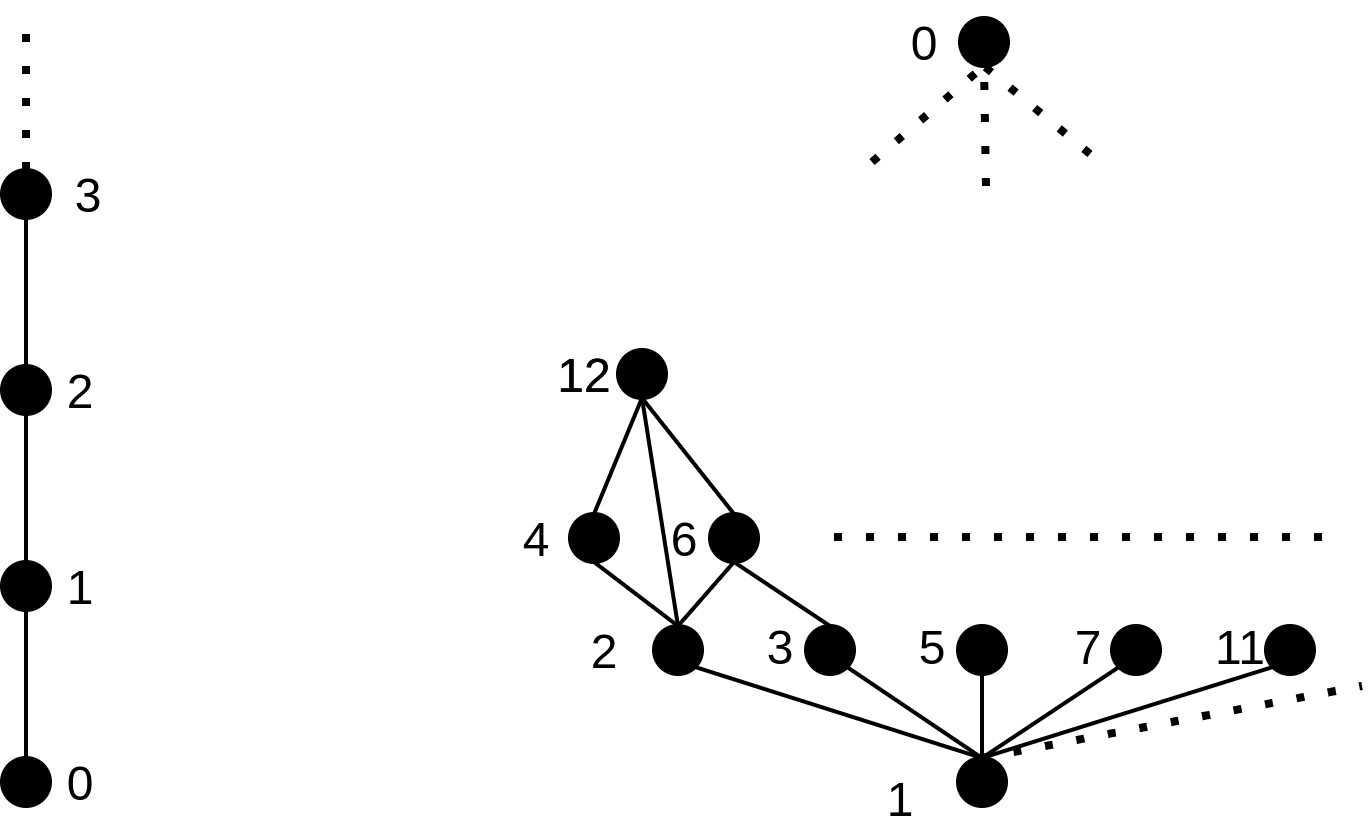
\includegraphics[width=0.5\textwidth]{images/reticolo2.png}
  \caption{Due relazioni d'ordine.}
  \label{figure:relazionireticoli}
\end{figure}

Nella Figura \ref{figure:relazionireticoli} si può vedere una rappresentazione 
(tramite reticoli, definiti a seguire) delle due relazioni d'ordine. 
La prima, quella totale, è rappresentata a destra: si può notare come sia 
``lineare'' a confronto della seconda, parziale, che è rappresentata a 
sinistra: quest'ultima infatti si dirama: alla base ha $1$, il numero che 
divide tutti gli altri; al primo ``strato'' ha tutti i numeri primi, 
il secondo i multipli dei multipli dei numeri primi (che saranno comunque collegati 
ai numeri primi, in quanto saranno divisibili anche per essi) e, commettendo 
un abuso che solitamente viene concesso, in cima vi è il numero $0$ che è divisibile 
da tutti gli altri, benché non sia divisibile per sé stesso. 

\subsubsection{Reticoli}
Un insieme $P$ con una relazione d'ordine (parziale) $\leq$, 
notato $(P, \leq)$ è detto insieme parzialmente ordinato 
o, in inglese, partially ordered set (\textit{poset}). 
L'insieme delle classi di equivalenza 
delle formule è un insieme parzialmente ordinato con delle peculiarità. 

Tra tutti i \textit{poset}, ci interessano quelli con alcune particolari proprietà 
strutturali, chiamati \textbf{reticoli}. 

\begin{figure}[!h]
  \centering 
  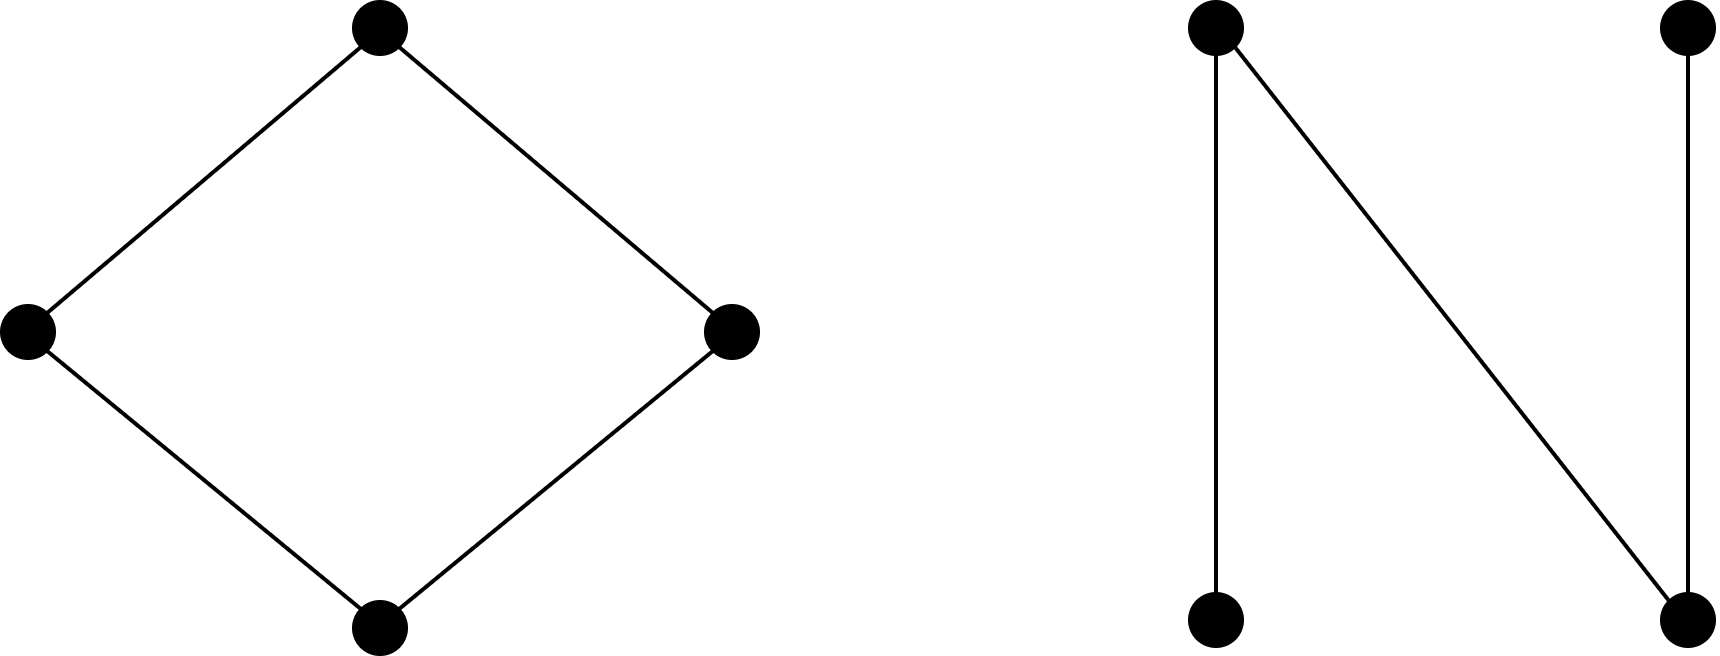
\includegraphics[width=0.5\textwidth]{images/reticolo.png}
  \caption{Due reticoli.}
  \label{figure:reticolo}
\end{figure}


La Figura \ref{figure:reticolo} riporta due immagini. 
Non entrambi sono reticoli: quello più a destra, infatti, non lo è. 
Cosa li distingue? La proprietà strutturale (più importante per i nostri 
scopi) che li divide, è che per quello più a sinistra, il reticolo, data 
ogni qualsiasi coppia di elementi possibile, si può sempre trovare 
quale dei due sia il minimo elemento che è più grande della coppia e il 
massimo elemento che è più piccolo della coppia. Questo non avviene nell'altro 
caso, infatti i due elementi ``in alto'', non hanno un minimo elemento 
più grande di loro, mentre i due elementi ``in basso'' non hanno un massimo 
elemento più piccolo di loro. In altre parole, non hanno 
\textbf{estremi inferiori} ed \textbf{estremi superiori}, che sono 
invece la proprietà fondamentale dei reticoli. 

Si definiscono quindi questi due concetti. 

\begin{defi}[Estremo inferiore]
  Dati due elementi $x, y$ appartenenti ad un insieme parzialmente ordinato $(P, \leq)$, si definisce 
  $$
  \inf(\{x,y\}) = \max\{z \in (P, \leq): z \leq x \text{ e } z \leq y\}
  $$
\end{defi}
e analogamente si definisce 
\begin{defi}[Estremo superiore]
  Dati due elementi $x, y$ appartenti ad un insieme parzialmente ordinato $(P, \leq)$, si definisce 
  $$
  \sup(\{x,y\}) = \min\{z \in (P, \leq): x \leq z \text{ e } y \leq z\}
  $$
\end{defi}
Si possono generalizzare $\inf()$ e $\sup()$ da un sottoinsieme $S \subseteq P$, con 
$P$ poset $(P, \leq)$:
\begin{align*}
  \inf(S) = \max\{z \in & (P, \leq): z \leq s\ \forall s \in S\} & \text{max dei minoranti di } S \\
  \sup(S) = \min\{z \in & (P, \leq): s \leq z\ \forall s \in S\} & \text{min dei maggioranti di } S \\
\end{align*}
A questo punto si può definire il minimo di un sottoinsieme (e analogamente il massimo), se esiste, come: 
\begin{align*}
  \min(S) := z \in S : z = \inf(S) &&
  \max(S) := z \in S : z = \sup(S)
\end{align*}
Si può ora definire formalmente un reticolo: 
\begin{defi}[Reticolo come poset]
Un reticolo è un insieme parzialmente ordinato $(R, \leq) : \forall x, y \in R$ esistono $\inf(\{x,y\})$ e $\sup(\{x,y\})$. 
\end{defi}

\noindent 
Dopo aver definito i reticoli, si definisce un'ulteriore struttura, necessaria per concludere l'argomento dell'Algebrizzazione della Logica Booleana. 

\subsection{Struttura Algebrica}
\begin{defi}
Dato un insieme $S$ e le operazioni $*_1, *_2, \cdots, *_n$ delle operazioni su $S$, allora $(S, *_1, *_2, \cdots, *_n)$ è una \textbf{struttura algebrica}.
\end{defi} 
\begin{defi}
  Visto come una struttura algebrica, un reticolo è $(R, \sqcup, \sqcap)$, con $\sqcup, \sqcap$ operazioni $\sqcup: R^2 \rightarrow R$ e $ \sqcap: R^2 \rightarrow R$, tale che le due operazioni siano commutative, associative e valga l'assorbimento.
\end{defi}
\begin{lem}
Ogni reticolo visto come insieme parzialmente ordinato è anche una struttura algebrica
$$
(R, \leq) \iff (R, \sqcup, \sqcap)
$$
\end{lem}
\begin{proof}
  ($\Longrightarrow$) con $R\equiv R,\ \forall a,b \in R$, siano:
  \begin{align*}
     a \sqcap b := \inf \{a,b\} && a \sqcup b := \sup \{a,b\}
  \end{align*}
  visto che si può verificare che per $\inf()$ e $\sup()$ valgono le proprietà di commutatività, assorbimento e associatività.
  
  ($\Longleftarrow$) con $R \equiv R$ definiamo $\forall a,b \in R$:
  \begin{align*}
    a \leq b \text{ sse } a = a \sqcap b &&
    b \leq a \text{ sse } a = a \sqcup b
  \end{align*}
  $(R, \leq)$ è quindi un poset, infatti si può verificare che $\leq$ è riflessiva, antisimmetrica e transitiva~(\ref{def:poset}). \\
  $(R, \leq)$ è anche un reticolo perché $\forall a,b \in R$ esiste $\inf$ e $\sup$: sia $c \leq a$ e $ c \leq b$
  \begin{align*}
    & c \leq a \text{ e } c \leq b \\
    \iff & c = c \sqcap a \text{ e } c = c \sqcap b & \text{per def. } \leq \\
    \iff & c = (c \sqcap b) \sqcap a \\
    \iff & c = c \sqcap (b \sqcap a) & \text{per associatività} \\
    \iff & c \leq b \sqcap a & \text{per def. } \leq \\
    \iff & c \leq \inf\{b, a\} & \text{per def. } \inf()
  \end{align*}
  Per il $\sup$ si ragiona in modo analogo. 
\end{proof}


\subsection{Definizione di Algebra Booleana}
A questo punto, siamo finalmente pronti per definire cosa sia l'Algebra Booleana.
\begin{defi}[Algebra Booleana]
L'Algebra Booleana è un sistema $(S, \sqcap, \sqcup, 0, 1, ()^c)$ di operazioni tali che $(S,\sqcup,\sqcap)$ sia un reticolo limitato, complementato, distributivo:
\begin{itemize}
  \item \textbf{limitato}: $\forall a \in S$:
    \begin{align*}
      & a \sqcup 0 = a & (a \geq 0) \\
      & a \sqcap 1 = a & (a \leq 1)
    \end{align*}
  \item \textbf{complementato}: $\forall a \in S$
    \begin{align*}
      a \sqcap a^c = 0 && a \sqcup a^c = 1
    \end{align*}
  \item \textbf{distributivo}: $\forall a,b, c \in S$:
    \begin{align*}
      a \sqcap (b \sqcup c) = (a \sqcap b) \sqcup (a \sqcap c) && a \sqcup (b \sqcap c) = (a \sqcup b) \sqcap ( a \sqcup c)
    \end{align*}
\end{itemize}
\end{defi}

Un esempio è il seguente: dato un insieme $A$ si consideri 
$(P(A), \cup, \cap, \emptyset, A, ()^c)$ e si ha 
$(P(A), \subseteq)$ tale che $A \subseteq B \iff A = A \cap B$. 

\paragraph{Esercizio}
Si dimostri che le seguenti sistemi siano un'algebra booleana:
\begin{itemize}
  \item $(F(A), \cup, \cap, \emptyset, A, ()^c)$ \\
    con $A$ un insieme infinito, e $F(A)$ l'insieme dei suoi sottoinsiemi finiti o complementi di insiemi finiti
  \item $(\{0,1\}, \min, \max, 0, 1, 1-\_)$
\end{itemize}

\subsubsection{Algebra di Lindenbaum}
L'algebra delle formule, chiamata anche \textbf{Algebra di 
Lindenbaum delle Formule}, è definita come 
$$
(\mathscr{F_L}/_{\equiv}, \land, \lor, \bot, \top, \neg)
$$
Dato che $\equiv$ è una congruenza, si possono definire le seguenti operazioni con $A,B \in \mathscr{F_L}$:
\begin{align*}
  [A]_{\equiv} \land [B]_{\equiv} & = [A \land B]_{\equiv} \\
  [A]_{\equiv} \lor [B]_{\equiv} & = [A \lor B]_{\equiv} \\
  [A]_{\equiv} \rightarrow [B]_{\equiv} & = [A \rightarrow B]_{\equiv} \\
  \neg [A]_{\equiv} & = [\neg A]_{\equiv} \\
  [\top]_{\equiv} & = \text{ tautologie} \\
  [\bot]_{\equiv} & = \text{ contraddizioni} \\
\end{align*}
La cardinalità dell'insieme delle classi di equivalenza scrivibili con $n$ variabili è:
$$
|\mathscr{F_L}^{(n)}/_\equiv| = 2 ^ {2^n} = |\{F: \{0,1\}^n \rightarrow \{0,1\}\}| = |\mathscr{P}(\{1,\cdots,2^n\})|
$$

\subsection{Funzioni Termine}
Al fine di arrivare ad un discorso completo sulle Forme Normali, si continua a ragionare sulle classi d'equivalenza delle formule e la loro struttura, ora da un punto di vista che sembra essere diverso ma che in conclusione si riunirà con quanto detto precedentemente. 

Si rifletta sul significato di 
\begin{align}
\label{fun:formula-computazionale}
\models F \iff \forall \mathcal{v}: \mathscr{L} \rightarrow \{0,1\},\ \mathcal{v}(F) = 1
\end{align}
in termini ``computazionali'' significa \textit{tenere fermo} l'argomento ($F$) e far cambiare le funzioni. Sarebbe comodo scambiare i ruoli: la formula si comporta come una funzione che prende come argomenti gli assegnamenti.

Siano $A \in \mathscr{F_L}$ una formula e $n \in \mathbb{N}$. Le lettere proposizionali che occorrono in $A$ si indicano con
$$
Var(A) \subseteq \mathscr{L} \subseteq \{p_1, p_2, \cdots, p_n\}
$$
Sia ora $\hat{A}$ una \textbf{funzione termine} $\hat{A} : \{0,1\}^n \rightarrow \{0,1\}$ tale che:
$$
\forall \mathcal{v}:\mathscr{L} \rightarrow \{0,1\},\ \hat{A}(\mathcal{v}(p_1), \mathcal{v}(p_2), \cdots, \mathcal{v}(p_n)) = \widetilde{\mathcal{v}}(A)
$$

\begin{defi}[Funziona Termine]
Definizione di $\hat A : \{0,1\}^n \rightarrow \{0,1\}$ induttiva su $A$:
\begin{itemize}
  \item \textbf{base}: Se $ A = p_i$, con $p_i \in \{p_1, p_2, \cdots, p_n\}$ un letterale:
  $$\hat A := \hat{p_i} : \{0,1\}^n \rightarrow \{0,1\}$$
  con $\hat{p_i}(t_1, \cdots, t_n) = t_i$, l'$i$-esima proiezione. 
  Quindi $\forall \mathcal{v}: \mathscr{L} \rightarrow \{0,1\}$ si verifica che: 
  $$
  \hat{A} = \hat{p_i}(\mathcal{v}(p_1), \cdots, \mathcal{v}(p_n)) = \mathcal{v}(p_i) = \widetilde{\mathcal{v}}(p_i) = \widetilde{\mathcal{v}}(A)
  $$
\item \textbf{passo}: $\forall (t_1, \cdots, t_n) \in \{0,1\}^n$
  \begin{itemize}
    \item Se $A = \neg B$: $\hat{A}(t_1, \cdots, t_n) =  1 - \hat{B}(t_1, \cdots, t_n)$
    \item Se $A = B \land C$: $\hat{A}(t_1, \cdots, t_n) = \min \{\hat{B}(t_1, \cdots, t_n),\ \hat{C}(t_1, \cdots, t_n)\}$
    \item Se $A = B \lor C$: $\hat{A}(t_1, \cdots, t_n) = \max \{\hat{B}(t_1, \cdots, t_n),\ \hat{C}(t_1, \cdots, t_n)\}$
    \item Se $A = B \rightarrow C$: $\hat{A}(t_1, \cdots, t_n) = \max \{1 - \hat{B}(t_1, \cdots, t_n),\ \hat{C}(t_1, \cdots, t_n)\}$
  \end{itemize}
\end{itemize}
\end{defi}
\noindent
Ora si possono vedere come \textit{funzioni termine} la riflessione iniziale~(\ref{fun:formula-computazionale}): 
$$
\models F \iff \hat{F}(t_1, \cdots, t_n) = 1,\ \forall (t_1, \cdots, t_n)
$$
e l'equivalenza logica: 
$$
[F]_{\equiv} = [G]_{\equiv} \iff F \equiv G \iff \hat{F}(t_1, \cdots, t_n) = \hat{G}(t_1, \cdots, t_n),\ \forall t_i \in \{0,1\}^n
$$
Allo stesso modo si può dare una definizione diversa di Algebra Booleana, \textit{isomorfa} all'Algebra di Lindenbaum.
\begin{defi}[Algebra Booleana su Funzioni Termine sui primi $n$ termini]
$$
\hat{\mathscr{F}}_\mathscr{L}^{(n)} = (\{\hat{A}: \{0,1\}^n \rightarrow \{0,1\}, A \in \mathscr{F_L}\}, \land, \lor, \neg, \bot, \top) 
$$
dove i significati degli operatori sono quelli espressi nella definizione di funzioni termine. 
\end{defi}

\subsection{Teorema di Completezza Funzionale}
Concentriamoci sull'algebra $\hat{\mathscr{F}}_\mathscr{L}^{(n)}$ appena espressa e una $Funz^{(n)}$ definita come:
$$
Funz^{(n)} = (\{f: \{0,1\}^{(n)} \rightarrow \{0,1\}\}, \land, \lor, \neg, \bot, \top)
$$
Che rapporto sussiste tra le due Algebre?
Per ogni $n \in \mathbb{N}$, la prima ha come universo l'insieme di tutte le Funzioni Termine per ogni formula $A \in \mathscr{F_L}$, mentre la seconda ha come universo tutte le funzioni $f: \{0,1\}^n \rightarrow \{0,1\}$. \\
Sicuramente, data la restrizione, si può affermare che:
$$
\hat{\mathscr{F}}_\mathscr{L}^{(n)} \subseteq Funz^{(n)}
$$
Si dimostra, ora, che vale anche:
$$
\hat{\mathscr{F}}_\mathscr{L}^{(n)} \supseteq Funz^{(n)}
$$
Questo fatto prende il nome di \textbf{Teorema di Completezza Funzionale}. 
A parole, ciò che afferma è che ogni funzione $f: \{0,1\}^n \rightarrow \{0,1\}$ è esprimibile come una formula $F \in \mathscr{F_L}$. \\
Chiaramente, se dimostrato, vuol dire che le due algebre sono in realtà \textit{isomorfe}. 
\begin{teo}[di Completezza Funzionale]
$$
  \mathscr{\hat{F}_L}^{(n)} \supseteq Funz^{(n)},\ \forall n \in \mathbb{N}
$$
\end{teo}

La dimostrazione consiste nel fornire per ogni $n \in \mathbb{N}$ e ogni funzione $f: \{0,1\}^{n} \rightarrow \{0,1\}$ una formula \textit{costruibile} $F \in \mathscr{F_L}^{(n)} : f = \hat F$. 
\begin{proof}
Sia $f: \{0,1\}^{n} \rightarrow \{0,1\}$ una funzione, la cui cardinalità del dominio è $2^{n}$. Per ogni combinazione degli $n$ argomenti $(a_{i_1}, a_{i_2}, \cdots, a_{i_n})$ esiste un valore $b_i \in \{0,1\}$ associato:
\begin{align}
  f :=
  \begin{cases}
    (a_{1_1}, a_{1_2}, \cdots, a_{1_j}, \cdots, a_{1_n}) & \longrightarrow b_1 \\
    (a_{2_1}, a_{2_2}, \cdots, a_{2_j}, \cdots, a_{2_n}) & \longrightarrow b_2 \\
    ~~~~~~~~~~~~~~~     \vdots           & ~~~~~~~~ \vdots \\
    (a_{i_1}, a_{i_2}, \cdots, a_{i_j}, \cdots, a_{i_n}) & \longrightarrow b_i \\
    ~~~~~~~~~~~~~~~     \vdots           & ~~~~~~~~ \vdots \\
    (a_{(2^n)_1}, a_{(2^n)_2}, \cdots, a_{(2^n)_j}, \cdots, a_{(2^n)_n}) & \longrightarrow b_{(2^n)}
  \end{cases}
\end{align}
Costruiamo una formula $F \in \mathscr{F_L}$ in modo tale che $ \hat{F} = f$.
\begin{itemize}
  \item se $f(t_1, \cdots, t_n) = 0$ per ogni $(t_1, \cdots, t_n)$: $F = \bot$
  \item altrimenti sia $I \subseteq \{1, 2, \cdots, 2^{n}\}$ tale che:
  $$
  i \in I \iff b_i = 1
  $$
  (intuitivamente, $I$ contiene i numeri delle ``righe'' della tabella di verità della funzione $f$ in cui l'immagine è il numero $1$). \\
  Per ogni $i \in I$ si considera la $i$-esima tupla $(a_{i_1}, a_{i_2}, \cdots, a_{i_n})$ di argomenti di $f$. \\
  Per ogni $j \in \{1, \cdots, n\}$ si definisce:
  \begin{align*}
  A_{ij} =
  \begin{cases}
    p_j & \text{se } a_{ij} = 1 \\
    \neg p_j & \text{se } a_{ij} = 0
  \end{cases} &&
  \text{con } A_{ij} \in \mathscr{F_L}^{(n)}
  \end{align*}
  Si pone $F = \bigvee\limits_{i \in I}\bigwedge\limits_{j \in n} A_{ij}$
  
  Si mostra che $\hat{F} = f$, ovvero che per ogni riga $i \in I$:
  $$
  {[ \bigwedge\limits_ {j = 1}^{n} \hat{A}_{ij}(t_1, \cdots, t_n) ]} = 1
  \iff (t_1, \cdots, t_n) = (a_{i_1}, \cdots, a_{i_n})
  $$
  Infatti
  \begin{itemize}
  \item se $(t_1, \cdots, t_n) = (a_{i_1}, \cdots, a_{i_n})$, $\forall j \leq  n$:
    \begin{align*}
      \hat A_{ij}(t_1, \cdots, t_n) = t_j =
      \begin{cases*}
        \mathcal{v}(p_j) = a_{i_j} \\
        \mathcal{v}(\neg p_j) = 1 - a_{i_j}
      \end{cases*}
      &
      \begin{rcases*}
        \text{ se } a_{i_j} = 1 \\
        \text{ se } a_{i_j} = 0
      \end{rcases*} = 1
    \end{align*}
  \item se $(t_1, \cdots, t_n) \neq (a_{i_1}, \cdots, a_{i_n})$, $\exists t_j \neq a_{i_j}$:
    \begin{align*}
      \hat A_{ij}(t_1, \cdots, t_n) = t_j =
      \begin{cases*}
        \mathcal{v}(p_j) = a_{i_j} \\
        \mathcal{v}(\neg p_j) = 1 - a_{i_j}
      \end{cases*}
      &
      \begin{rcases*}
        \text{ se } a_{i_j} = 0 \\
        \text{ se } a_{i_j} = 1
      \end{rcases*} = 0
    \end{align*}
  \end{itemize}
  Quindi $(A_{i_1} \land A_{i_2} \land \cdots \land A_{i_n})$ può essere resa vera solo da un assegnamento. In definitiva, 
  $$
  \hat{F} = \bigvee\limits_{i\in I}\bigwedge\limits_{j}^n \hat A_{i_j}(t_1, \cdots, t_n) = 1 \iff (t_1, \cdots, t_n) \text{ è la riga } i \text{-esima, e } i \in I
  $$
  Quindi $\hat F = f$.  
\end{itemize}
\end{proof}

\subsubsection{Considerazioni sul Teorema di Completezza Funzionale}
Per come è stato provato il Teorema di Completezza Funzionale, la funzione termine si può anche esprimere come: 
$$
G = \bigwedge\limits_{i \in J} \bigvee_{j = 1}^{n} B_{ij}
$$
con
\begin{align*}
  J \subseteq \{0, \cdots, 2^n-1\} &&
  i \in J \iff b_j = 0 &&
  B_{ij} =
  \begin{cases}
    \neg p_j & a_{ij} = 1 \\
    p_j & a_{ij} = 0 \\
  \end{cases}
\end{align*}
Si ha, quindi, che $\hat{F} = f = \hat{G}$\footnote{Ciò che è stato fatto è esattamente uguale alla costruzione dei minterm e maxterm per una data tavola di verità.}, il che è una dimostrazione che una qualsiasi formula può essere messa in una \textbf{forma normale} perché $\hat{\mathscr{F}}_\mathscr{L}^{(n)} = Funz^{(n)}$.

Sebbene il Teorema possa sembrare banale, in quanto la sua dimostrazione è
semplice, il suo contenuto non è nullo né scontato. Un esempio di mancanza 
funzionale è già presente nella Logica Proposizionale stessa, nonostante 
la dimostrazione precedente, rimuovendo il vincolo su $n$ e definendo
$$
Funz^{\omega} := \{f:\{0,1\}^{\omega} \rightarrow \{0,1\}\}
$$
con $\omega = |\mathbb{N}|$, in altre parole l'insieme di tutte le successioni 
infinite di valori $\{0,1\}$. Se valesse il Teorema di Completezza Funzionale 
anche in questo caso, si dovrebbe poter affermare che tale insieme 
è incluso nelle classi di equivalenza scritte nelle classi di equivalenza 
delle formule scritte con $\omega$ variabili: 
$$
Funz^{\omega} \subseteq \hat{\mathscr{F}}_\mathscr{L}^{\omega} = \mathscr{F_L}^{\omega}/_\equiv
$$
Ma in realtà
$$
|Funz^{\omega}| = |\mathbb{R}| \geq |\mathbb{N}| = |\mathscr{F_L}^{\omega}/_\equiv|
$$
e pertanto non è valido. 

\paragraph{Forme Normali Canoniche}
Le forme normali che abbiamo trovato non sono desiderabili per gli scopi 
futuri, in quanto sono molto prolisse: ognuno degli $A_{ij}$ menziona 
tutte le lettere proposizionali $p_1, \cdots, p_n$ (analogamente per le 
forme congiuntive) ed è infatti chiamata Forma Normale Disgiuntiva (or di and) \textbf{Canonica} o \textbf{Completa}. \\
Si noti la prolissità nel costruire una $F \in \mathscr{F_L}$ t.c. $\hat F = f : \{0, 1\}^3 \rightarrow \{0, 1\}$ con: 
$$
f(t_1, t_2, t_3) = t_1 ~~~ \forall (t_1, t_2, t_3)
$$
È chiaro che la formula più ``corta'' è $F = t_1$, ma con la forma 
canonica si rappresenta come:
$$
F = (p_1 \land \neg p_2 \land \neg p_3) \lor (p_1 \land \neg p_2 \land p_3) \lor (p_1 \land p_2 \land \neg p_3) \lor (p_1 \land p_2 \land p_3)
$$

\paragraph{Insieme funzionalmente completo di connettivi}
C'è un'altra nozione, legata alla Completezza Funzionale, che è molto interessante, 
ossia la nozione di \textit{insieme funzionalmente completo di connettivi}. 
\begin{defi}[Insieme funzionalmente completo di connettivi]
Un insieme 
  $$
  C \subseteq \{\land, \lor, \rightarrow, \neg, \leftrightarrow, \bot, \top\}
  $$
è definito \textit{funzionalmente completo} se per ogni $F \in \mathscr{F_L}$ esiste una $G \in \mathscr{F_L}$ scritta usando solo i connettivi in $C$ tale che $F \equiv G$ e $\hat{F} = \hat{G}$, ossia $[F]_{\equiv} = [G]_{\equiv}$. 
\end{defi}

Un insieme di connettivi funzionalmente 
completo è dato dal Teorema di Completezza Funzionale stesso, ossia 
$C = \{\land, \lor, \neg\}$. Si può mostrare facilmente che 
anche $\{\neg, \land\}$ e $\{\neg, \lor\}$ sono completi (in quanto, grazie alle 
leggi di De Morgan, $(A \lor B) = \neg (\neg A \land \neg B)$). Questi non 
sono gli unici insiemi funzionalmente completi: 
$\{\neg, \rightarrow\}$ (in quanto $(A \land B) \equiv \neg (A \rightarrow \neg B)$ 
e $(A \lor B) \equiv ((\neg A) \rightarrow B)$ 
e $\{\rightarrow, \bot\}$. In particolare, un insieme composto da un 
solo connettivo, il \texttt{nand}, è anch'esso funzionalmente completo, 
in quanto ogni altro connettivo è ricostruibile utilizzando solo 
$$
A \barwedge B = \neg (A \land B)
$$
infatti $\neg A \equiv A \barwedge A$ e, ovviamente, $A \land B \equiv \neg ( A \barwedge B)$ 
per definizione. 

\section{Forme Normali}
Dopo averle introdotte col Teorema di Completezza Funzionale, possiamo 
passare ad un esame più approfondito delle Forme Normali.
Le Forme Normali Congiuntive e Disgiuntive Canoniche sono 
esageratamente prolisse. Sarebbe utile conservare l'idea delle Forme Normali 
con formule più succinte. 

\subsection{Forma Normale Negata}
Una terza forma normale, chiamata \textbf{Negation 
Normal Form} (NNF) che, per definizione, è l'insieme delle formule 
che rispettano le seguenti proprietà: 
\begin{itemize}
  \item non contiene $\rightarrow$ 
  \item $\neg$ occorre solo applicato a lettere proposizionali
\end{itemize}
quindi, per esempio 
\begin{align*}
p_1 \land \neg(p_2 \lor p_3) \notin NNF \\
p_1 \land (\neg p_2 \lor \neg p_3) \in NNF
\end{align*}

\begin{defi}[Sottoformula]
$G$ è sottoformula di $F$ sse $G$ occorre in ogni $\mathscr{L}$-costruzione di $F$ e si indica con $G \preccurlyeq F$
\end{defi}

\begin{lem}
Ogni formula $F \in \mathscr{F_L}$ è equivalente a una $F^{N} \in NNF$. 
\end{lem}
\begin{proof}
Per provare il lemma, descriviamo come trasformare $F$ in $F^{N}$ in un numero 
finito di passi, dove ogni passo produce una formula equivalente alla precedente. 
Per ottenere la sequenza si applica ad ogni passo una delle seguenti 
trasformazioni a $G \preccurlyeq F$:

\begin{enumerate}
  \item $C \rightarrow D \leadsto (\neg C) \lor D$
  \item $\neg \neg C \leadsto C$
  \item $\neg(C \lor D) \leadsto \neg C \land \neg D$
  \item $\neg (C \land D) \leadsto \neg C \lor \neg D$
\end{enumerate}

Un'osservazione preliminare su questo algoritmo è che si può mostrare che applicando 
le quattro regole in un ordine qualsiasi si ottiene sempre $F^{N} \in NNF$. 
Si mostrerà che partendo da $(1)$ e applicando le altre trasformazioni si possa 
arrivare a $F^{N}$: sia data $F \in \mathscr{F_L}$. In un numero finito di applicazioni 
di $(1)$ si ottiene una $F'$ in IFNF (Implication-Free Normal Form), equivalente 
a $F$. 

Si introduce una misura di \textit{distanza}: si definisce 
$i(E)$ come il numero di connettivi $\rightarrow$ nella formula $E$. 
Si ha, quindi, 
che $E \in IFNF \iff i(E) = 0$. Inoltre, se $E \notin IFNF$, allora 
$E'$ ottenuta applicando $(1)$ su $E$ deve avere $i(E) > i(E')$.\\
È chiaro che $F \equiv F'$ poiché l'applicazione di $(1)$ è semplicemente 
l'applicazione di una equivalenza eseguita grazie al Teorema di Sostituzione. 
Quindi, in un certo numero di passi  si ha
$$ 
F = F_0 \equiv \cdots \equiv F' (\in IFNF) \equiv F_i \equiv \cdots \equiv F_n (\in NNF)
$$
e si nota che le applicazioni di $(2)$, $(3)$ e $(4)$ trattano tutte equivalenze logiche. Ciò che bisogna dimostrare è che la sequenza di trasformazioni termini, ossia l'algoritmo non è infinito ($n \in \mathbb{N}$).

Per dimostrare che l'algoritmo termina, siano ora $A,E \in \mathscr{F_L}$ e si definisce $\ell(A) = $ ``n° di occorrenze di connettivi in $A$''.
Definiamo quindi $m(E)$ come la somma del numero di connettivi presenti nelle sottoformule $\neg A$ di $E$: 
$$
m(E) = \sum_{\neg A \preccurlyeq E} \ell(A)
$$
Si noti che 
$$
m(E) = 0 \iff E \in NNF
$$
Infatti:
\begin{itemize}
  \item  se $E \in NNF$:
    \begin{align*}
      & \forall \neg A \preccurlyeq E,\ A \in \mathscr{L} & \text{per def. } NNF\\
      \iff & \forall \neg A \preccurlyeq E,\ \ell(A) = 0 \\
      \iff & m(E) = 0
    \end{align*}
  \item se $m(E) = 0$:
    $$
    \sum_{\neg A \preccurlyeq E} \ell(A) = 0 \iff \forall \neg A \preccurlyeq E,\ \ell(A) = 0 \iff \forall \neg A \preccurlyeq E,\ A \in \mathscr{L}
    $$ 
\end{itemize}
In un passaggio eseguito con una delle $(2), (3), (4)$ generando 
$$
E \leadsto E'
$$
si ha che $m(E) > m(E')$. Se si riesce a dimostrare quest'ultima affermazione, 
allora si dimostra automaticamente che il procedimento termina in un numero 
finito di passi. 
\paragraph{(2) $\neg \neg C \leadsto C$}: In questo caso
\begin{align*}
  \begin{cases}
        m(\neg \neg C) & = \ell(\neg C) + m(\neg C)
                         = \ell(C) + 1 + \ell(C) + m(C) \\
                       & = 1 + 2 \cdot \ell(C) + m(C) \\
        m(C)
  \end{cases}
\end{align*}
$$
  \implies m(\neg \neg C) > m(C)
$$

\paragraph{(3) $\neg (C \lor D) \leadsto \neg C \land \neg D$}: In questo caso
\begin{align*}
  \begin{cases}
    m(\neg (C \lor D)) & = \ell(C \lor D) + m(C) + m(D) \\
                       & = \ell(C) + \ell(D) + m(C) + m(D) + 1 \\
    m(\neg C \land \neg D) 
                       & = \ell(C) + \ell(D) + m(C) + m(D)
  \end{cases}
\end{align*}
$$
  \implies m(\neg (C \lor D)) > m(\neg C \land \neg D)
$$
Analogamente per $(4)$.

Data una formula $F \in \mathscr{F_L}$, si può costruire una successione 
finita 
$$ 
F = F_0 \equiv \cdots \equiv F' (\in IFNF) \equiv F_i \equiv \cdots \equiv F_n (\in NNF)
$$
e ovviamente $F \equiv F_n$, per un qualche $n \in \mathbb{N}$. 
\end{proof}

\subsection{Forma Normale Congiuntiva e Disgiuntiva}
Le CNF o FNC, Forme Normali Congiuntive, sono un sovrainsieme delle CNF \textit{complete} o canoniche.
\begin{defi}[Letterale]
Un \textit{letterale} è una formula nella forma $p$ o $\neg p$ per qualche lettera proposizionale $p$ (i.e., o è una lettera proposizionale o è la sua negata).
La definizione di \textbf{letterale opposto} a uno dato è, dato $A$ letterale, l'opposto di $A$:
$$
\bar{A} = 
\begin{cases}
  \neg p & \text{se } A = p \\
  p & \text{se } A = \neg p
\end{cases}
$$
\end{defi}
\begin{defi}[Clausola]
Una \textit{clausola} è una disgiunzione di un numero finito $k$ di letterali:
$$
\ell_1 \lor \ell_2 \cdots \lor \ell_k
$$
dove ogni $\ell_i$ è un letterale. 
\end{defi}
\begin{defi}[CNF o FNC]
Una \textbf{forma normale congiuntiva} è una congiunzione di un numero finito $h$ di 
clausole: 
$$
C_1 \land C_2 \land \cdots \land C_h
$$
dove ogni $C_j$ è una clausola. 
\end{defi}
\begin{defi}[Clausola vuota]
Una \textbf{clausola vuota} $\qedsymbol$ è definita come la disgiunzione 
di zero letterali. 
\end{defi}

Questo concetto è importante e non va confuso col concetto 
di \textbf{CNF vuota} $\emptyset$, definita come la congiunzione di zero clausole. 
Prendendo una sequenza di letterali e formule
\begin{align*}
F_0 & = \qedsymbol \\
F_1 & = \ell_1 \\
F_2 & = \ell_1 \lor \ell_2 \\
F_3 & = \ell_1 \lor \ell_2 \lor \ell_3 \\
\vdots \\
F_i & = \ell_1 \lor \ell_2 \lor \ell_3 \lor \cdots \lor \ell_i
\end{align*}
possiamo notare che ogni assegnamento che soddisfa una formula $F_i$, soddisfa anche quella successiva $F_{i+1}$. Per questo $F_i \rightarrow F_{i+1}$ è una tautologia. \\
Seguendo questa definizione la clausola vuota è insoddisfacibile e pertanto è $\qedsymbol \equiv \bot$.

Per l'insieme di CNF vuote, si ha 
\begin{align*}
& \emptyset \\
& C_1 \\
& C_1 \land C_2 \\
& C_1 \land C_2 \land C_3\\
& \vdots \\
& C_1 \land C_2 \land C_3 \land C_4
\end{align*}
qui, al contrario, ogni assegnamento che soddisfa una clausola $C_i$, soddisfa anche la precedente $C_{i-1}$. \\
Seguendo questa definizione la CNF vuota è soddisfacibile ed è, in realtà, soddisfatta da ogni assegnamento: $\emptyset \equiv \top$. 

\begin{defi}[DNF o FND]
Una \textit{forma normale disgiuntiva} è una disgiunzione di un numero finito $n$ di formule:
$$
D_1 \lor D_2 \lor \cdots \lor D_n
$$
dove ogni $D_i$ è una congiunzione chiamata \textbf{co-clausola} di un numero finito $v$ di letterali:
$$
\ell_1 \land \ell_2 \land \cdots \land \ell_v
$$
\end{defi}

DNF si tratta, quindi, di una struttura duale rispetto alle CNF.
Si noti la terminologia speciale per le CNF: questa terminologia è riservata alle CNF in quanto la dualità tra CNF e DNF verrà spezzata. 

\begin{lem}
Ogni formula $F \in \mathscr{F_L}$ è logicamente equivalente a una formula $F^c \in CNF$ 
e a una formula $F^d \in DNF$.
\end{lem}

Questo è già stato dimostrato grazie al teorema di completezza funzionale, che tuttavia utilizzava le CNF e DNF complete. 
\begin{proof}[esistenza DNF/CNF]
Per induzione strutturale su $F$:
\begin{itemize}
  \item \textbf{base}: se $F = p$ con $p \in \mathscr{L}$ allora $p = p^c = p^d$.
  \item \textbf{passo}:
    \begin{itemize}
      \item se $F = \neg G$, per ipotesi induttiva si ha $G^c \equiv G$ e $G^d \equiv G$. 
        Allora, se
        \begin{align*}
           G = C_1 \land C_2 \land \cdots \land C_h &&
          \text{dove ogni } C_i = \ell_{i_1} \lor \cdots \lor \ell_{i_{k_i}}
        \end{align*}
        si ha che:
        \begin{align*}
          \neg G \equiv \neg (G^c) & \equiv \neg (C_1 \land \cdots \land C_h) \\
                   & \equiv \neg C_1 \lor \neg C_2 \lor \cdots \lor \neg C_h := (\neg G)^d & \text{per DeMorgan}
        \end{align*}
        \begin{align*}
          \text{dove ogni } \neg C_i & \equiv \neg (\ell_1 \land \ell_2 \land \cdots \land \ell_v) \\
                               & \equiv \neg \ell_{i_1} \land \cdots \land \neg \ell_{i_{k_i}} & \text{per DeMorgan} \\
                               & \equiv \bar \ell_{i_1} \land \cdots \land \bar \ell_{i_{k_i}} & \neg \ell_{i_j} \text{ è } \equiv \text{ a un letterale opposto} \\
          \implies (\neg G)^d \in DNF 
        \end{align*}
        e similmente:
        \begin{align*}
          \neg G \equiv \neg (G^d) & \equiv \neg (D_1 \lor \cdots \lor D_n) \\
                   & \equiv \neg D_1 \land \neg D_2 \land \cdots \land \neg D_n := (\neg G)^c & \text{per DeMorgan}
        \end{align*}
        \begin{align*}
          \text{con } \neg D_i & \equiv \neg (\ell_{i_1} \land \cdots \land \ell_{i_{k_i}}) \\
                               & \equiv \neg \ell_{i_1} \land \cdots \land \neg \ell_{i_{v_i}} & \text{per DeMorgan} \\
                               & \equiv \bar \ell_{i_1} \land \cdots \bar \neg \ell_{i_{v_i}} & \neg \ell_{i_j} \text{ è } \equiv \text{ a un letterale opposto} \\
          \implies (\neg G)^c \in CNF 
        \end{align*}
        Quindi esistono sia $F^d := (\neg G)^d \equiv \neg (G^c)$ che $F^c := (\neg G)^c \equiv \neg (G^d)$. 
      \item se $F = (G \land H)$, per ipotesi induttiva si ha:
        \begin{align*}
           G^c \equiv G && G^d \equiv G \\
           H^c \equiv H && H^d \equiv H
        \end{align*}
        Si definisce, allora
        \begin{itemize}
          \item $F \equiv F^c$ \\
                con $F^c := (G^c \land H^c)$ e, banalmente $(G^c \land H^c) \in CNF$
          \item $F^d$:
            \begin{align*}
              F & \equiv (G^d \land H^d) \\ 
                & \equiv (G_1 \lor \cdots \lor G_u) \land (H_1 \lor \cdots \lor H_v) \\
                & \equiv \bigvee\limits_{i,j}(G_i \land H_j) & \text{per Distributività Generalizzata}~(\ref{def:distributibilita-generalizzata})
            \end{align*}
            Ma visto che $C_i$ e $H_j$ sono \textit{co-clausole}, anche $(G_i \land H_j)$ lo è.
            $$
            \implies F^d := \bigvee\limits_{i=1}^u \bigvee\limits_{j=1}^v (G_i \land H_i) \in DNF
            $$
        \end{itemize}
      \item se $F = (G \lor H)$, per ipotesi induttiva si ha:
        \begin{align*}
          G^c \equiv G && G^d \equiv G \\
          H^c \equiv H && H^d \equiv H
        \end{align*}
        Si definisce, allora
        \begin{itemize}
          \item $F \equiv F^d$ \\
                con $F^d := (G^d \lor H^d)$ e, banalmente $(G^d \lor H^d) \in DNF$
          \item $F^c$:
            \begin{align*}
              F & \equiv (G^c \lor H^c) \\ 
                & \equiv (G_1 \land \cdots \land G_u) \lor (H_1 \land \cdots \land H_v) \\
                & \equiv \bigwedge\limits_{i,j}(G_i \lor H_j) & \text{per Distributività Generalizzata}~(\ref{def:distributibilita-generalizzata})
            \end{align*}
            Ma visto che $C_i$ e $H_j$ sono \textit{clausole}, anche $(G_i \lor H_j)$ lo è.
            $$
            \implies F^c := \bigwedge\limits_{i=1}^u \bigwedge\limits_{j=1}^v (G_i \lor H_i) \in CNF
            $$generalizzata
        \end{itemize}       
      \item se $F = (G \rightarrow H)$, ci si comporta analogamente contando che $F \equiv (\neg G \lor H)$      
    \end{itemize}
\end{itemize}
\end{proof}

Si nota, tuttavia, che muoversi tra DNF e CNF con la distributività generalizzata causa un notevole allungamento delle formule. Per esempio:
\begin{align*}
        \bigvee\limits_{i = 1}^{n} (p_i \land q_i) \equiv \bigwedge\limits_{i = 1}^{2^n}(\ell_{i_1} \lor \cdots \lor \ell_{i_n})
\end{align*}
quindi c'è una dilatazione esponenziale. Questo è un bel problema.


Ci sono algoritmi più intelligenti per generare da DNF delle formule CNF più corte? \\
Purtroppo no. 

\chapter{Complessità Computazionale e Deduzione Automatica}

In questo momento, per decidere se una formula $F \in \mathscr{F}_\mathscr{L}$ che menziona $n$ lettere proposizionali diverse sia soddisfacibile o meno, l'algoritmo che conosciamo computa la sua tabella di verità, analizzando quindi $2^n$ possibilità, ossia un numero esponenziale. 
qui
Cominciamo definendo cosa sia un problema di decisione:
\begin{defi}[Problema di Decisione]
Dato $\Sigma^*$ un insieme di tutte le \textit{parole} finite costruite coi simboli di $\Sigma$—un \textit{alfabeto} finito—e un \textit{Linguaggio} $L \subseteq \Sigma^*$, non necessariamente finito, il problema di decisione consiste nel verificare se una stringa finita $w$ appartenga o meno al Linguaggio $L$
\end{defi}

Ad esempio, fissato 
$$
\Sigma = \{\land, \lor, \neg, \rightarrow, (, ), p, |\}
$$
si possono definire alcuni problemi, per esempio
$$
\mathscr{F}_\mathscr{L} \subseteq \Sigma ^*
$$
dove il problema risiede nel capire se una certa formula di lunghezza finita
risiede in $\mathscr{F}_\mathscr{L}$ oppure no. 
Vi sono dei problemi principalmente di natura sintattica, come appunto $\mathscr{F}_\mathscr{L}$ 
ma anche $NNF$, $CNF$ e $DNF$. Vi sono problemi in cui la natura semantica 
è decisiva, per esempio $SAT$, dove 
$$
w \in \Sigma^* : w\in SAT \iff w \in \mathscr{F}_\mathscr{L} \land w \text{ è soddisfacibile}
$$
oppure $TAUTO$, dove una stringa finita appartiene a $TAUTO$ sse è una formula ed è una tautologia, ossia
$$
w \in \Sigma^* : w \in TAUTO \iff w \in \mathscr{F}_\mathscr{L} \land \models w
$$
e analogamente $UNSAT$, il problema di decidere se una certa formula è
insoddisfacibile.

\section{Complessità Computazionale}
\subsection{Efficienza}
Alcuni dei problemi elencati precedentemente possono essere risolti (decisi) 
in maniera efficiente, ossia data una \textit{parola} $w$ decidere se 
appartiene ad un certo linguaggio: esempi di soluzioni efficienti sono 
quelle che riguardano tutti i problemi sintattici, risolvibili in tempo 
al massimo quadratico e in realta anche lineare con alcune tecniche di parsing. 

I problemi che riguardano la semantica, invece, sono tipicamente più complessi
da risolvere e infatti, per quanto conosciamo fino ad ora, si possono risolvere 
solo (nel caso peggiore) con un analisi dell'intera tabella di verità della 
formula, quindi con un numero esponenziale di calcoli. \`E importante rimarcare 
nuovamente che benché sussista questa difficoltà, verificare che 
un singolo assegnamento verifichi la formula è invece un calcolo semplice 
che richiede un tempo decisamente più contenuto rispetto al problema di 
decidibilità.

Quindi, vi sono dei problemi decidibili efficientemente, 
dei problemi decidibili molto difficilmente e verificabili facilmente 
e dei problemi decidibili molto difficilmente e verificabili difficilmente; 
da qui parte una gerarchia di classi di complessità infinita, ma a noi interesseranno 
solo le prime due. 
 
Per essere più precisi, si fissa un modello astratto di computazione, che fornisca 
la nozione di \textit{passo elementare}, in modo da poter ragionare precisamente 
sull'efficienza dei problemi. 
Qualunque modello di computazione che costituisca un modello realistico 
di calcolatore, con associata una nozione di passo elementare per costruire 
algoritmi, classifica i problemi nello stesso modo. 

\begin{oss}[Tesi di Church-Turing]
  Ogni modello ragionevole di computazione è equivalente.
\end{oss}

Uno dei modelli di computazione è quello delle Macchine di Turing (MdT): un'idea 
della Macchina di Turing è immaginarla come una macchina che lavora su un 
nastro infinito in lettura e scrittura, mantenendo uno stato e operando su 
una singola porzione di nastro in lettura utilizzando un programma per 
muoversi tra gli stati e scrivere sul nastro. 

Si può passare ora alla definizione formale delle classi dei problemi: 
\begin{defi}[Classe $\mathbb{P}$]
  La classe dei problemi ``efficientemente decidibili'' è definita, con una 
  certa ideologia sottesa, come tutti quei problemi che possono essere 
  risolti in tempo polinomiale, ossia esiste una certa Macchina di Turing T 
  e un polinomio $p: \mathbb{N}\rightarrow \mathbb{N}$ per i quali per ogni 
  $w \in \Sigma^*$  la computazione della MdT sull'input $w$, 
  denotato $T(w)$ termina entro $p(||w||)$ passi e per ogni $w \in L$ si 
  ha che $T(w)$ accetta il problema e per ogni $w \notin L$  si ha 
  che $T(w)$ non accetta, ossia risolve il problema.
\end{defi}

\begin{defi}[Classe $\mathbb{NP}$]
  La classe dei problemi ``verificabili efficientemente'' è definita come 
  tutti quei problemi tali per cui esiste una Macchina di Turing deterministica 
  e due polinomi $p,q:\mathbb{N}\rightarrow \mathbb{N}$ tali che per ogni 
  $w \in \Sigma^*$ e ogni $z \in \Gamma^*$, ossia un \textbf{certificato}, 
  che si può immaginare prodotto da un oracolo, si ha 
  che $T(w,z)$ termina entro $p(||w||)$ passi e si ha che per ogni 
  $w \in L$ esiste $z \in \Gamma^*$ tale che $||z|| \leq q(||w||)$ (ossia 
  il certificato è sufficientemente corto) e $T(w,z)$ accetta e per ogni 
  $w \notin L$ si ha che per ogni possibile $z \in \Gamma^*$ sufficientemente corto
  $T(w,z)$ rifiuta, ossia ``valida'' il certificato.
\end{defi}

\begin{defi}[Riducibilità]
        Un problema $L_1 \subseteq \Sigma^*$ è \textbf{riducibile in tempo polinomiale} 
        a un altro problema $L_2 \subseteq \Gamma^*$ se e solo se esistono
        una Macchina di Turing $T_{{L_1}, {L_2}}$ e un polinomio
        $p: \mathbb{N} \rightarrow \mathbb{N}$ tale che per ogni $w \in L_1$
        $T(w)$ trasfroma $w$ in $w' \in \Gamma^*$ in un numero di passi 
        minore o uguale a $p(||w||)$. 
\end{defi}

Per indicare la relazione di riducibilità tra due problemi si indica la notazione 
$L_1 \preceq_p L_2$ per indicare che il primo problema è riducibile polinomialmente 
al secondo; la nozione di riducibilità è utile poiché rende possibile risolvere 
istanze del problema $L_1$ ``riscrivendole'' come se fossero istanze di $L_2$
(chiaramente questa utilità si verifica quando è più facile risolvere $L_2$ di 
$L_1$). 
Un esempio di riducibilità polinomiale è 
$$
TAUTO \preceq_p UNSAT
$$
poiché la trasformazione $w \rightarrow \neg w$ è semplice e si sa che 
$w$ è tautologica se e solo se $\neg w$ è insoddisfacibile.

\begin{defi}[Problemi $\mathbb{NP}$-completi]
        Un problema appartenente alla classe $\mathbb{NP}_c$ è un problema 
        $L \subseteq \Sigma^*$ se e solo se 
        \begin{itemize}
                \item $L \in \mathbb{NP}$
                \item ogni $L' \in \mathbb{NP}$ è tale che $L' \preceq_p L$ 
        \end{itemize}
        La seconda proprietà si chiama $\mathbb{NP}$-hardness. 
\end{defi}
Come corollario della definizione dei problemi $\mathbb{NP}_c$, si ha che risolvendo 
polinomialmente un problema di tale classe si dimostra che 
$$
\mathbb{P} = \mathbb{NP}
$$

\begin{teo}[di Cook-Levin]
        $CNFSAT \in \mathbb{NP}$-completo.
        ($\implies SAT \in \mathbb{NP}$-completo)
\end{teo}

$CNFSAT \preceq_p SAT$ è vero perché una formula in CNF è comunque ancora una formula e pertanto la trasformazione—i.e., la funzione identità—è ovviamente polinomiale.\\
Si mostra ora che $SAT \preceq_p CNFSAT$, conservando non l'equivalenza logica ma la \textit{relazione di equisoddisfacibilità}.
Questo ci permetterà anche di trasformare polinomialmente le $DNF$ in $CNF$ equisoddisfacibili. Infattibile se si cercasse di mantenere l'$\equiv$.

\subsection{Equisoddisfacibilità}
\begin{defi}[Equisoddisfacibilità]
Siano $A, B \in \mathscr{F}_\mathscr{L}$. $A$ e $B$ sono equisoddisfacibili ($equisodd$) sse:
$$
A\ sodd. \iff B\ sodd.
$$
ossia se $A$ e $B$ sono entrambe soddisfsacibili o entrambe insoddisfacibili. 
\end{defi}

\subsubsection{Osservazioni sull'equisoddisfacibilità}
\begin{ossn}
L'equivalenza implica l'equisoddisfacibilità, ma non è vero il contrario.
\begin{enumerate}
\item Date le due formule $\neg (A \land B)$ e $\neg A \lor \neg B$, è noto 
che sono equivalenti grazie alle leggi di De Morgan e sono, di conseguenza, 
anche equisoddisfacibili.
\item $\neg (A \land B)$ e $(\neg A \land \neg B)$ non sono equivalenti, 
infatti l'assegnamento $A=1$ e $B=1$ soddisfa solo una delle due, tuttavia 
sono equisoddisfacibili.
\item $A \land \neg A$ e $\neg A \land \neg B$ non sono né equivalenti né
equisoddisfacibili.
\end{enumerate}
\end{ossn}

\begin{ossn}
$equisodd.$ è un tipo di relazione d'equivalenza:
\begin{itemize}
  \item $A\ equisodd.\ A$
  \item $A\ equisodd.\ B$, quindi $B\ equisodd.\ A$
  \item $A\ equisodd.\ B$ e $B\ equisodd.\ C$, quindi $A\ equisodd.\ C$
\end{itemize}
\end{ossn}

\begin{ossn}
$equisodd.$ non è una congruenza rispetto ai connettivi, pensati come operazioni. \\
Per esempio, rispetto a $\neg$: \\
se $A\ equisodd. B$ con $\models A$ e $\nvDash B$ (i.e. $B$ non è tautologica), allora vuol dire che $\neg A$ \textbf{non} è $equisodd.$ con $\neg B$—perché $A \in \bot$ ma $B$ potrebbe essere soddisfacibile.
\end{ossn}

\begin{ossn} $equisodd.$ è più grezza di $\equiv$, infatti le classi di equivalenza delle formule su $n$ variabili $\mathscr{F}_\mathscr{L}^{(n)}/\equiv$, sono $2^{2^n}$. \\
L'equisoddisfacibilità, invece, ha unicamente due classi: l'insieme delle formule insoddisfacibili ($[\bot]$) e tutte le rimanenti, ossia tutte quelle soddisfacibili da almeno un assegnamento.
\end{ossn}
Quest'ultima osservazione era deducibile anche dalla Osservazione 1.

\subsection{Riduzione $SAT \preceq CNFSAT$}
Sia $A \in \mathscr{F}_\mathscr{L}$ tale che $A$ sia in Negation Normal Form, ossia $A \in NNF$. \\
Se $A \notin CNF$, allora contiene almeno una violazione, ovvero una sottoformula del tipo $C \lor (D_1 \land D_2)$ oppure $(D_1 \land D_2) \lor C$ (c'è un $\land$ interno ad un $\lor$).

Senza perdita di generalità trattiamo, d'ora in poi, solo il primo dei due casi. Sia $A \in NNF$, ogni sua violazione $B = C \lor (D_1 \land D_2)$ si sostituisce con una nuova lettera proposizionale $a \in L$ che ancora non è presente in $A$. Si crea quindi $B'$ tale che:
\begin{align*}
B' := B'' \land (\neg a \lor D_1) \land (\neg a \lor D_2)
&&
\text{con } B'' := B[a/D_1\land D_2]
\end{align*}

Si osservi che $(\neg a \lor D_1) \land (\neg a \lor D_2) \equiv a \rightarrow (D_1 \land D_2)$. \\
\begin{lem}
$B'$ e $B$ sono equisoddisfacibili, ma in genere non sono equivalenti.\\
E $B'$ ha $2n + 1$ clausole, di cui $1$ di $n$ letterali e $2n$ di $2$ letterali .
\end{lem}
\begin{proof}[Dimostrazione $B \in SAT \implies B' \in SAT$]
        Per ipotesi, dato che $B$ è soddisfacibile, sia $\mathcal{v}:\mathscr{L} \rightarrow \{0,1\}$
        tale che $\mathcal{v}(B) = 1$, ossia $\mathcal{v} \models B$. 
        Si definisce 
        $$
        \mathcal{v}_a: \mathscr{L} \rightarrow \{0,1\} = 
        \begin{cases}
                \mathcal{v}_a(p) = \mathcal{v}(p) & \forall p \in L, p \neq a \\
                \mathcal{v}_a(a) = \mathcal{v}(D_1 \land D_2) 
        \end{cases} 
        $$
        L'assegnamento $\mathcal{v}_a$ è ben definito, nel senso che non 
        da alla stessa lettera proposizionale due assegnamenti diversi.
        Si nota che $\mathcal{v}_a \models a \rightarrow (D_1 \land D_2)$, 
        dato che per definizione $\mathcal{v}_a(a) = \mathcal{v}(D_1 \land D_2)$
        e per interpretazione dell'implicazione $0 \rightarrow 0 = 1$ e 
        $1 \rightarrow 1 = 1$; dunque:
        \begin{align}
        \label{dim:b'-equiv-b''}
        \mathcal{v}_a(B') = \mathcal{v}_a(B'' \land a \rightarrow (D_1 \land D_2)) = \mathcal{v}_a(B'') \land 1 = \mathcal{v}_a(B'')
        \end{align}
        $B$ e $B''$ si possono riscrivere come: 
        \begin{align*}
        B & = B''[D_1 \land D_2/a] & \text{dato che } a \text{ non appare in } B \\
        B'' & = B''[a/a]
        \end{align*}
        e grazie al Lemma~\ref{lem:sostituzione} di Sostituzione si può affermare che $\mathcal{v}_a(B) = \mathcal{v}_a(B'')$ in quanto $\mathcal{v}_a(a) = \mathcal{v}_a(D_1 \land D_2)$. \\
        Quindi:
        \begin{align*}
                1 &= \mathcal{v}(B) & \text{ipotesi } \\
                  &= \mathcal{v}_a(B) & a \text{ non occore in } B \\
                  &= \mathcal{v}_a(B'') & \text{per il Lemma di Sost.}  \\
                  &= \mathcal{v}_a(B') & \text{per~\ref{dim:b'-equiv-b''}}
        \end{align*}
        ossia l'assegnamento che soddisfa $B$ soddisfa anche $B'$, ossia 
        sono equisoddisfacibili. 
\end{proof}
\begin{proof}[Dimostrazione $B' \in SAT \implies B \in SAT$]
        Se $B'$ è soddisfacibile da un assegnamento della forma $\mathcal{v}_a$—ossia tale che $\mathcal{v}_a(a) = \mathcal{v}(D_1 \land D_2)$—allora si può tranquillamente ribaltare la catena di uguaglianze precedente: 
        \begin{align*}
          \mathcal{v}_a \models B' \text{ sse }1 &= \mathcal{v}_a(B') \\
          &= \mathcal{v}_a(B'') & \text{per~\ref{dim:b'-equiv-b''}}  \\
          &= \mathcal{v}_a(B) & \text{per il Lemma di Sost.} \\
          \text{sse } & \mathcal{v}_a \models B
        \end{align*}
        Si supponga, ora, che $B'$ sia soddisfatto solo da assegnamenti $\mathcal{w}$ che non sono della forma $\mathcal{v}_a$, ossia $\mathcal{w}(a) \neq \mathcal{w}(D_1 \land D_2)$. Vi sono allora due casi:
        \begin{itemize}
          \item $\mathcal{w}(a) = 0 \neq \mathcal{w}(D_1 \land D_2) = 1$
          \item $\mathcal{w}(a) = 1 \neq \mathcal{w}(D_1 \land D_2) = 0$
        \end{itemize}
        Tuttavia quest'ultimo caso è impossibile, poiché $\mathcal{w}(a \rightarrow D_1 \land D_2) = 1 \rightarrow 0 = 0 = \mathcal{w}(B')$ e quindi $\mathcal{w}$ non soddisferebbe $B'$.
        
        Quindi rimane il primo caso e bisogna mostrare che effettivamente soddisfa $B'$ e non porta ad un assurdo
        
        \begin{oss}
        Sia $E$ un'espressione formata solo da $0, 1, \land, \lor$—interpretabili come $\min$ e $\max$. Il valore di $E$, quindi, è o $0$ o $1$. \\
        Sia $E'$ ottenuta da $E$ rimpiazzando nessuna o più occorrenze  del simbolo $0$ con $1$. \\
        Allora $E \leq E'$.
        
        Questo perché $0, 1, \min, \max$ sono tutte funzioni non decrescenti, e $E$ ed $E'$ sono composizioni di funzioni non decrescenti, pertanto sono non decrescenti neanche loro. \\
        (un'altra prova è per induzione strutturale su $E$).
        \end{oss}

        Ora, tornando al problema principale, si ha che:
        \begin{align*}
        \mathcal{w}(B') = 1 &&
        \mathcal{w}(a) = 0 &&
        \mathcal{w}(D_1 \land D_2) = 1
        \end{align*}
        Se $Var(B) = \{p_1,\cdots p_n\}$, allora $\mathcal{w}(B)$ e $\mathcal{w}(B'')$ si possono esprimere come funzioni termine di $B''$:
        \begin{align*}
        \mathcal{w}(B'') & = \hat{B}''(\mathcal{w}(p_1), \cdots, \mathcal{w}(p_n), \mathcal{w}(a)) \\
        \mathcal{w}(B) & = \hat{B}''(\mathcal{w}(p_1), \cdots, \mathcal{w}(p_n), \mathcal{w}(D_1 \land D_2)) & \text{per def. } B''
        \end{align*}
        Dato che la formula iniziale $A$ era in $NNF$, anche $B''$, $B'$ e $B$ lo sono, e $\mathcal{w}(B'')$ e $\mathcal{w}(B)$ sono quindi considerabili come espressioni costruite su $0,1,\land,\lor$, per l'osservazione precedente. \\
        Si può concludere, quindi, che
        $$
        \mathcal{w}(B'') = \hat{B}''(\mathcal{w}(p_1), \cdots, \mathcal{w}(p_n), 0) \leq \hat{B}''(\mathcal{w}(p_1), \cdots, \mathcal{w}(p_n), 1) = \mathcal{w}(B)
        $$
        ma $\mathcal{w}(B'') = 1$, quindi $\mathcal{w}(B) = 1$ 
\end{proof}

\begin{oss}[Nota finale]
        Si sarebbe potuto definire $B'$, alternativamente, come segue: 
        \begin{align*}
                B' :&= B[a/D_1 \land D_2] \land (a \leftrightarrow (D_1 \land D_2))^c \\
                   &=  B[a/D_1 \land D_2] \land (\neg a \lor D_1) \land (\neg a \lor D_2) \land ((D_1 \land D_2) \rightarrow a)^c \\
                   &=  B[a/D_1 \land D_2] \land (\neg a \lor D_1) \land (\neg a \lor D_2) \land (a \lor \neg D_1 \lor \neg D_2)
        \end{align*}
        Nella prova di $B' \in SAT \implies B \in SAT$ si sarebbe potuto mostrare che $B'$ è soddisfatto solo da assegnamenti nella forma di $\mathcal{v}_a$ tali che $\mathcal{v}_a(a) = \mathcal{v}(D_1\land D_2)$.
\end{oss}

\paragraph{Dilatazione della riduzione $NNF$-$CNF$}
Nel passaggio da $B$ a $B'$ si osserva una dilatazione nella lunghezza della formula, ossia $B'$ è \textit{più lungo} di $B$; data la formula 
generale 
$$
B' := B[a/D_1 \land D_2] \land (\neg a \lor D_1) \land (\neg a \lor D_2)
$$
La parte che subisce la sostituzione può essersi accorciata, a cui però si aggiungono una decina di simboli. Quindi $||B'|| \leq ||B|| + k$, con $k$ una costante dipendente dal modo in cui si conta la lunghezza (si contano le parentesi come simboli eccetera). \\
Per ogni ``violazione'' $B$ nella formula originale $A$, la formula risultante equisoddisfacibile senza violazioni è più lunga di $k \cdot v$ caratteri, con $v =$ \#violazioni. \\
Inoltre, visto che in $A$ non può essere più lunga di $v$, la formula risultante $A'$ avrà lunghezza $||A'|| \leq ||A|| + k \cdot v \leq (k + 1) \cdot ||A||$, una dilatazione \textit{lineare}.

La tecnica usata per ridurre $SAT \preceq_p CNFSAT$ che consiste nel rimpiazzare 
$B$ con $B'$ equisoddisfacibile è ispirata alla riduzione 
$$
SAT \preceq_p 3CNFSAT
$$
dovuta a Karp. Il passaggio $B \implies B'$ è un esempio del cosiddetto 
``Tseytin's Trick'', che si usa per ridurre $F \in \mathscr{F}_\mathscr{L}$ a una 
in $3CNFSAT$ ad essa equisoddisfacibile. 

\begin{defi}[Problemi $3CNFSAT$]
$3CNFSAT \subseteq CNFSAT \subseteq \mathscr{F}_\mathscr{L}$ è costituito da tutte e sole le CNF dove ogni clausola contiene esattamente $3$ letterali. \\
$3CNFSAT \in \mathbb{NP}$-completo.
\end{defi}
\begin{oss}[Problemi $2CNFSAT$]
        $2CNFSAT \in \mathbb{P}$.
\end{oss}
\begin{algorithm}
\caption{Algoritmo di riduzione a CNF equisoddisfacibili}
\begin{algorithmic} 
\REQUIRE $F \in \mathscr{F}_\mathscr{L}$
\ENSURE $A \in CNF : F\ equisodd.\ A$
\STATE {$A : A \in NNF \land A \equiv F$}
\WHILE{$A \notin CNF$}
\STATE $B \leftarrow$ violazione in $A$
\STATE $B' \leftarrow B[a/D_1 \land D_2] \land (\neg a \lor D_1) \land (\neg a \lor D_2)$ ~~~~~~~~~~~~~~~~~~~~~~~~~~~~~~~~~~~~~~ con $a \notin Var(B)$
\STATE $A \leftarrow A[B/B']$
\ENDWHILE
\RETURN{$A$}
\end{algorithmic}
\end{algorithm}

\subsubsection{Esempi}
\paragraph{1} Sia $A := p \lor (q \land r)$ in $NNF$. Si trasforma ora in una formula equisoddisfacibile in CNF: 
$$
A' := (p \lor a) \land (\neg a \lor q) \land (\neg a \lor r)
$$
Queste due formule non sono equivalenti, infatti vi sono assegnamenti 
che portano a risultati diversi; tuttavia sono equisoddisfacibili.

\paragraph{2} 
Sia $A := (p_1 \land p_2) \lor (p_2 \land q_2) \lor (p_3 \land q_3)$. Applicando iteramente la sostituzione, si ha:
\begin{align*}
(a_1 \lor (p_2 \land q_2) \lor (p_3 \land q_3)) & \land (\neg a_1 \lor p_1) \land (\neg a_1 \lor q_1) \\
(a_1 \lor a_2 \lor (p_3 \land q_3)) & \land (\neg a_1 \lor p_1) \land (\neg a_1 \lor q_1) \land (\neg a_2 \lor p_2) \land (\neg a_2 \lor p_2) \\
(a_1 \lor a_2 \lor a_3) & \land (\neg a_1 \lor p_1) \land (\neg a_1 \lor q_1) \land (\neg a_2 \lor p_2) \land (\neg a_2 \lor q_2) \land (\neg a_3 \lor p_3) \land (\neg a_3 \lor q_3)
\end{align*}
Data una formula con $n$ letterali si generano $2 \cdot n +1 $ clausole, 
di cui una con $n$ letterali e $2n$ con due letterali, laddove utilizzando la 
distributività se ne generavano $2^n$ ognuna con $n$ letterali. 


\section{Deduzione Automatica}
Ricordiamo che noi vorremmo studiare $\Gamma \stackrel{?}{\models} A$, che si può ricondurre ad un problema di soddisfacibilità o al suo complementare di insoddisfacibilità. Tuttavia:
\begin{align*}
  & \mathbb{NP}\text{-complete} \ni SAT \preceq_p CNFSAT \\
  & \text{co}\mathbb{NP}\text{-complete} \ni TAUTO \preceq_p SAT^c \preceq_p CNFUNSAT
\end{align*}

Il motivo per cui non studiamo invece $DNFSAT$ e $DNFUNSAT$—che sono in $\mathbb{P}$—è che $SAT \npreceq_p DNFSAT$. Non c'è un algoritmo per ``tradurre'' una formula arbitraria equisoddisfacibile in $DNF$ in modo che sia sufficientemente corta: i metodi conosciuti allungano esponenzialmente la formula.

\begin{defi}[Variazione notazionale]
Date $F_i \in \mathscr{F}_\mathscr{L}$, le formule 
\begin{align*}
  F_1 \land F_2 \land \cdots \land F_k &&
  F_1 \lor F_2 \lor \cdots \lor F_k
\end{align*}
si possono scrivere senza parentesi grazie all'associatività, si possono scambiare le formule interne nelle formule esterne ($F_1 \land F_2 \equiv F_2 \land F_1$) grazie alla commutatività e, infine, si possono espandere le singole formule ($F_1 \land F_1  \equiv F_1$) grazie all'idempotenza.

Per questo motivo d'ora in poi per le $CNF$ tralasceremo gli operatori $\land$ e $\lor$ in favore di una notazione insiemistica. Per esempio:
\begin{align*}
  (p \lor q \lor \neg r) \land &(q \lor r \lor a) \land p \\
  & \Downarrow \\
  \{ \{p, q, \neg r\}, &\{q, r, a\}, \{p\}\}
\end{align*}
Una teoria costituita da CNF è indicata come l'insieme di tutte le clausole appartenenti a qualche CNF della teoria (di fatto è una CNF più grande). Inoltre:
\begin{align*}
  & \emptyset = CNF \text{ vuota} \\
  & \qedsymbol = \text{ clausola vuota} \\
  & \{\cdots, \qedsymbol, \cdots \} = CNF \text{ contenente la clausola vuota}.
\end{align*}
\end{defi}

Il problema di definire se $A$ è conseguenza logica di una teoria $\Gamma$ 
$$
\Gamma \stackrel{?}{\models} A
$$
si può ridurre a calcolare la insoddisfacibilità di $\Gamma \cup \{\neg A\}$, che è uguale a calcolare l'insoddisfacibilità della sua forma in CNF $S := \{\Gamma^c \cup \{\neg A\}^c\}$ dove $\Gamma^c := \{\gamma^c | \gamma \in \Gamma\}$ e $\{\neg A\}^c \in CNF$. 

Il problema $\Gamma \models A$ è stato ridotto polinomialmente al problema $S \in CNFSAT$,
dove $S$ è un insieme di clausole considerate come insiemi di letterali, 
eventualmente infinito.


\subsection{Metodi refutazionali}
$S$ è soddisfacibile se esiste $\mathcal{v}:\mathscr{L} \rightarrow \{0,1\}$ tale 
che per ogni clausola $C \in S, \mathcal{v} \models C$, in altre parole esiste un letterale $\ell \in C$ tale che $\mathcal{v} \models \ell$. 

Se l'obiettivo è dimostrare che $S$ è insoddisfacibile, una strategia 
può essere ampliare $S$ in un nuovo insieme $S \subseteq S'$ in modo 
tale che $S'$ è logicamente equivalente o almeno equisoddisfacibile a $S$.
Ad esempio, se ampliando iterativamente $S$ in $S'$, $S''$ fino a $S^{(u)}$ 
e alla fine la clausola vuota $\qedsymbol$ appartiene a $S^{(u)}$ allora quest'ultimo 
è insoddisfacibile, e quindi anche $S$ lo è. Questa idea può essere sfruttata 
disegnando \textbf{metodi refutazionali}, ossia metodi che hanno l'obiettivo di 
provare l'insoddisfacibilità di un insieme di clausole, in questo frangente, 
ma più in generale anche di una formula o una teoria. Questi metodi sono basati 
sulla regola di inferenza chiamata \textbf{principio di risoluzione}, 
il quale è utile per un tipo di calcolo particolarmente adatto a essere automatizzato, 
ossia SAT solver e Theorem Prover. 

\begin{defi}[Principio di Risoluzione]
        Date due clausole $C_1$ e $C_2$ si dice che $D$ è la \textbf{risolvente}
        di $C_1$ e $C_2$ sul pivot $\ell$ se e solo se
        \begin{itemize}
                \item $\ell \in C_1$
                \item $\bar{\ell} \in C_2$
                \item $D := (C_1 \setminus \{\ell\}) \cup (C_2 \setminus \{\bar{\ell}\})$
        \end{itemize}
       e si scriverà $D = \mathbb{R}(C_1,C_2; \ell, \bar{\ell})$. 
\end{defi}

\subsubsection{Esercizio}
Mostrare che $(C_1 \setminus \{\ell\}) \cup (C_2 \setminus \{\bar{\ell}\})$ può essere 
diverso da $(C_1 \cup C_2) \setminus \{\ell, \bar{\ell}\}$.

Sia $C_1 = \{a,\neg a\}$ e $C_2 = \{a, \neg a, b\}$. Allora
\begin{align*}
  (C_1 \setminus \{a\}) \cup (C_2 \setminus \{\neg a\}) & = \{a, \neg a, b\} \\
  (C_1 \cup C_2) \setminus \{a, \neg a\} & = \{b\}
\end{align*}
  

\subsubsection{Esempio}
Sia $C_1 := \{x, y, \neg t\}$ e $C_2 := \{u, \neg y, t\}$; si ha
\begin{align*}
D_1 & = \mathbb{R}(C_1, C_2; y, \neg y) = \{x, \neg t, u\} \\
D_2 & = \mathbb{R}(C_1, C_2; \neg t, t) = \{x, y, u, \neg y\}
\end{align*} 

\begin{lemn}[di correttezza della risoluzione]
\label{lem:correttezza-risoluzione}
        Sia $D = \mathbb{R}(C_1, C_2; \ell, \bar{\ell})$, allora 
        $$
        \{C_1, C_2\} \models D
        $$
\end{lemn}

\begin{proof}
Dimostriamo che $\mathcal{v} \models C_1$ e $\mathcal{v} \models C_2 \implies \mathscr{v} \models D$. \\
Sia $\mathcal{v} : \mathscr{L} \rightarrow \{0, 1\}$ tale che:
  \begin{align*}
    & \mathcal{v} \models C_1 \text{ e } \mathcal{v} \models C_2 \\
    \implies & \exists m \in C_1, n \in C_2 \text{ t.c. } \mathcal{v} \models m \text{ e } \mathcal{v} \models n \\
    & \text{Per assurdo assumiamo } m = \ell \text{ e } n = \bar \ell \\
    \implies & \mathcal{v}(\ell) = 1 \text{ e } \mathcal{v}(\bar \ell) =1 \\
    \implies & \bot \\
    \implies & m \neq \ell \text{ o } n \neq \bar \ell \\
    \implies &  m \in D \text{ o } n \in D \\
    \implies & \mathcal{v}(D) = 1
  \end{align*}
\end{proof}

\begin{cor}
        Se $\mathbb{R}(C_1, C_2; \ell, \bar{\ell}) = \qedsymbol$ allora 
        $\{C_1, C_2\}$ è insoddisfacibile, in quanto $\{C_1, C_2\} \models \qedsymbol$.
\end{cor}
\begin{defi}[\textit{Calcolo refutazionale basato su risoluzione}]
  Sia $S$ un insieme di clausole e sia $S := S_0, S_1, \cdots, S_k$ una successione di insiemi tale che per ogni $i = 0, \cdots, k-1$ si ha che $S_{i+1}$ si ottiene unendo a $S_i$ una o più risolventi di clausole in $S_i$. \\
  Se $\qedsymbol \in S_k$, allora $S$ è insoddisfacibile.
\end{defi}
L'obiettivo è mostrare che i calcoli refutazionali basati su applicazioni 
ripetute della risoluzione sono corretti e completi (refutazionalmente).
In genere, per un calcolo logico si studiano infatti le due
seguenti proprietà:
\begin{defi}[Correttezza]
        Un calcolo si definisce \textbf{corretto} se i certificati che produce 
        testimoniano il vero, ossia sono corretti, in altre parole 
        non produce certificati fasulli. 
\end{defi}

Per esempio, nel frangente attuale $S_0, S_1, \cdots, S_k \ni \qedsymbol$ è un certificato corretto dell'insoddisfacibilità di $S = S_0$. \\
Questo genere di calcolo è corretto, e la dimostrazione scende direttamente dal Lemma~\ref{lem:correttezza-risoluzione}, come vedremo tra poco.

\begin{defi}[Completezza]
        Un calcolo è completo se non omette alcun certificato. 
\end{defi}
Nella situazione attuale vuol dire che se $S$ è insoddisfacibile, allora esiste $S_0, S_1, \cdots, S_k$ tale che si produce $\qedsymbol \in S_k$.

Prima di mostrare che il calcolo refutazionale è completo, è necessario 
prepararsi la strada, poiché non sarà banale. 

\begin{teo}[Teorema di Completezza del principio di risoluzione (o di Robinson)]
Un insieme $S$ di clausole è insoddisfacibile $\iff \qedsymbol \in \mathscr{R}^*(S)$, dove $\mathscr{R}^*(S)$ è definito come segue:
\begin{align*}
  \mathscr{R}^0(S) &:= S \\
  \mathscr{R}^1(S) &:= S \cup \{D: D = \mathbb{R}(C_1, C_2; \ell, \bar{\ell})\} & \text{per qualche } C_1,C_2 \in S \text{ e } \ell \in C_1 \text{ e } \bar\ell \in C_2 \\
  \mathscr{R}^2(S) &:= \mathscr{R}(\mathscr{R}(S)) \\
  \cdots \\
  \mathscr{R}^{t+1}(S) &:= \mathscr{R}(\mathscr{R}^{t}(S)) \\
  \cdots \\
  \mathscr{R}^*(S) &:= \bigcup\limits_{i \in \omega} \mathscr{R}^i(S)
\end{align*} 
\end{teo}

Il calcolo $\mathscr{R}^*$ è un metodo \textit{a forza bruta}, applica il Principio di Risoluzione calcolando ciecamente tutte le risoluzioni possibili. Per questo non c'è da sperare che faccia molto meglio delle tavole di verità. 

\begin{proof}
\textit{Correttezza del calcolo $\mathscr{R}$: $\qedsymbol \in \mathscr{R}^*(S) \implies S$ insoddisfacibile} \\
\begin{align*}
& \qedsymbol \in \mathscr{R}^*(S) \\
\iff & \exists i \in \omega : \qedsymbol \in \mathscr{R}^i(S) & \text{per def. } \mathscr{R}^*(S) \\
\iff & \mathscr{R}^i(S)\ insodd. & \text{per def. di clausola vuota} \\
\iff & \mathscr{R}^i(S) \equiv \mathscr{R}^{i-1}(S) \equiv \cdots \equiv \mathscr{R}^0(S) = S & \text{per Lemma~\ref{lem:correttezza-risoluzione}} \\
\iff & S\ insodd.
\end{align*}
\end{proof}

\begin{proof}
\textit{Completezza Refutazionale del calcolo $\mathscr{R}$: $S \text{ insodd. } \implies \qedsymbol \in \mathscr{R}^*(S)$} \\
Dato che $S$ è insoddisfacibile, per il Teorema~\ref{thm:compattezza-prop} di Compattezza esiste un $S_{fin} \subseteq_{\omega} S$ finito e $S_{fin}$ è insoddisfacibile; 
bisogna capire come sia fatto $S_{fin}$: l'insieme finito $S_{fin}$ contiene un numero finito di lettere proposizionali $Var(S_{fin}) \subseteq \{p_1, p_2, \cdots, p_n\}$ per qualche $n \in  \omega$, $p_i \in \mathscr{L}$. \\
La notazione $C^{n}_\mathscr{L}$ indica l'insieme di tutte le clausole scrivibili sulle prime $n$ lettere proposizionali.
\begin{oss}
$S_{fin} \subseteq C^{n}_\mathscr{L}$ e $C^{0}_\mathscr{L} = \{ \qedsymbol \}$
\end{oss}
\textit{A fortiori}: dato che $S_{fin} \subseteq C^{n}_\mathscr{L}$, si ha $S_{fin} \subseteq (C^{n}_\mathscr{L} \cap S) \subseteq (C_\mathscr{L}^{n} \cap \mathscr{R}^*(S))$ e pertanto $C^{n}_\mathscr{L} \cap \mathscr{R}^*(S)$ è insodd., dato che $S_{fin}$ è insodd. \\
Dimostreremo, quindi, che $C^k_\mathscr{L} \cap \mathscr{R}^*(S) \text{ è insodd.}$ per ogni $ k = n, \cdots, 1,0$. Compreso, per $k = 0$:
$$
C^{0}_\mathscr{L} \cap \mathscr{R}^*(S) \text{ insodd. }
$$
Tuttavia dobbiamo capire com'è fatto $C^0_\mathscr{L} \cap \mathscr{R}^*(S)$:
$$
C^{0}_\mathscr{L} \cap \mathscr{R}^*(S) = 
\begin{cases}
  \emptyset  & \leadsto C^0_\mathscr{L} \cap \mathscr{R}^*(S) \text{ sodd. } \leadsto \bot \\
  \{\qedsymbol\} & \leadsto \text{ unico caso possibile }
\end{cases}
$$
Ma quindi, per def. di $\cap$, $\qedsymbol \in \mathscr{R}^*(S)$!

Per dimostrare che per ogni $k = n, \cdots, 1, 0$ 
$$
C^k_\mathscr{L} \cap \mathscr{R}^*(S) \text{ è insoddisfacibile} 
$$
si usa l'induzione decrescente su $k$:
\begin{itemize}
\item \textbf{base} ($k = n$): $C^n_\mathscr{L} \cap \mathscr{R}^*(S)$ insodd. (già dimostrato)
\item \textbf{passo} ($k-1$): si assume l'asserto vero per $n, n-1, \cdots, k$ e si dimostra per $k-1$, ossia 
$$
C^n_\mathscr{L} \cap \mathscr{R}^*(S), C^{n-1}_\mathscr{L} \cap \mathscr{R}^*(S), \cdots, C^k_\mathscr{L} \cap \mathscr{R}^*(S) \text{  insodd.}
$$

Per assurdo, si assuma $C^{k-1}_\mathscr{L} \cap \mathscr{R}^*(S)$ sodd., dunque esiste $\mathcal{v} \models C$ per ogni $C \in C^k_\mathscr{L} \cap \mathscr{R}^*(S)$; si definiscono ora 
\begin{align*}
\mathcal{v}^+ : \mathscr{L} \rightarrow \{0,1\},\ \mathcal{v}^+(p_k) = 1 \\
\mathcal{v}^- : \mathscr{L} \rightarrow \{0,1\},\ \mathcal{v}^-(p_k) = 0
\end{align*}
mentre per ogni altra $p_i \in C^k_\mathscr{L}$, $\mathcal{v}(p_i) = \mathcal{v}^+(p_i) = \mathcal{v}^-(p_i)$; si noti che $p_k \notin C^{k-1}_\mathscr{L}$. 
Per ipotesi induttiva esistono $C_1, C_2 \in C^k_\mathscr{L} \cap \mathscr{R}^*(S)$ insoddisfacibili, tali che:
\begin{align*}
\mathcal{v}^+(C_1) = 0 && \mathcal{v}^-(C_2) = 0
\end{align*}
La lettera proposizionale $p_k$ occorre in $C_1$, altrimenti vorrebbe dire che $C_1 \in C^{k-1}_\mathscr{L} \cap \mathscr{R}^*(S)$ e, visto che $C^{k-1}_\mathscr{L} \cap \mathscr{R}^*(S)$ è sodd. per ipotesi assurda, vorrebbe dire che $\mathcal{v}^+(C_1) = \mathcal{v}(C_1) = 1$. Assurdo. \\
Deve però apparire come letterale $\neg p_k$, così che $\mathcal{v}^+(C_1) = 0$ come da ipotesi. \\
Analogamente, $p_k$ occorre in $C_2$ e più precisamente come letterale positivo $p_k$ e la prova è identica, \textit{mutantis mutandis}. 

Dunque, esiste $D = \mathbb{R}(C_1, C_2; \neg p_k, p_k) = (C_1 \setminus \{ \neg p_k\}) \cup (C_2 \setminus \{p_k\})$, con:
\begin{align*}
& p_k, \neg p_k \notin D \\
\iff & D \in C^{k-1}_\mathscr{L} \cap \mathscr{R}^*(S) && \text{perché non compare } p_k \\
\iff & \mathcal{v}(D) = 1 && \text{per ipotesi assurda} \\
\iff & \mathcal{v} \models D
\end{align*}.

Vi sono due casi:
\begin{enumerate}
  \item $\mathcal{v}$ soddisfa qualche letterale in $C_1 \setminus \{\neg p_k\}$. Ma allora $\mathcal{v}(C_1) = 1$ e $\mathcal{v}^+(C_1) = 1$, assurdo.
  \item $\mathcal{v}$ soddisfa qualche letterale in $C_2 \setminus \{p_k\}$, e allora $\mathcal{v}^-(C_2) = 1$, assurdo.
\end{enumerate}
Non essendoci altri casi, si è raggiunta la contraddizione che conclude la dimostrazione per assurdo, dunque $C^k_\mathscr{L} \cap \mathscr{R}^*(S)$ è
insoddisfacibile per ogni $k$, $k=0$ incluso.
\end{itemize}
Dunque $C^0_\mathscr{L} \cap \mathscr{R}^*(S)$ è insoddisfacibile, pertanto $C^0 \cap \mathscr{R}^*(S) = \{\qedsymbol\}$ e $\qedsymbol \in \mathscr{R}^*(S)$.
\end{proof}
\begin{oss}
Se $S$ è un insieme finito di clausole, la costruzione di $\mathscr{R}^*(S)$ costituisce una \textit{procedura di decisione}, cioè sia che $S$ sia insodd. sia che $S$ sia sodd. termina in tempo finito, dando la risposta corretta.
\end{oss}
\begin{proof} Infatti, essendo $S$ finito, vengono usate solo un numero finito $n = |Var(S)|$ di lettere proposizionali diverse, dunque:
\begin{itemize}
  \item letterali scrivibili su $\{p_1, \cdots, p_n\}$: $2 \cdot n$
  \item letterali diversi che occorrono: $\leq 2 \cdot n$ 
  \item clasuole scrivibili su $2 \cdot n$ letterali: $\leq 2^{2 \cdot n}$
\end{itemize} 
In $S$, quindi, occorrono al più $2^{2 \cdot n}$ clausole. \\
Si nota, ora, che la risoluzione non introduce mai nuovi letterali, dunque la sequenza $\mathscr{R}^{0}(S) \subseteq R^1(S) \subseteq \cdots \mathscr{R}^{k}(S) \subseteq \cdots$ è tale che  che ogni $\mathscr{R}^{i}(S)$ è un sottoinsieme delle $2^{2 \cdot n}$ clausole 
scrivibili su $\{p_1, \cdots, p_n\}$. \\
Dunque esiste un $t \in \omega$ tale che $\mathscr{R}^{t}(S) = \mathscr{R}^{t+1}(S)$, poiché prima o poi tutte le clausole saranno contenute; 
pertanto
$$
\mathscr{R}^{t}(S) = \mathscr{R}^{t+1}(S) = \cdots = \mathscr{R}^*(S)
$$
Se si trova $\qedsymbol \in \mathscr{R}^i(S)$, si può concludere che $S$ sia insoddisfacibile. \\
Se, al contrario, $\mathscr{R}^t(S) = \mathscr{R}^{t+1}(S)$ e $\qedsymbol \notin \mathscr{R}^t(S)$, si può concludere che $S$ sia soddisfacibile perché non ci sono due clausole con due letterali opposti.
\end{proof}
\begin{oss}
Se, invece, $S$ è un infinito di clausole, dato un qualsiasi $S_{fin} \subseteq_\omega S$ esiste $t \in \omega$ tale che $\mathscr{R}^t(S_{fin}) = \mathscr{R}^{t+1}(S_{fin}) = \mathscr{R}^*(S_{fin})$, tuttavia questo non fornisce una procedura di decisione per $S$, ma esclusivamente di \textit{semidicesione}. Questo perché in genere non si sa ``scegliere'' $S_{fin}$ e il meglio che si può fare è, presa una successione infinita di sottoinsiemi infiniti
$$
S_1 \subseteq S_2 \subseteq \cdots \subseteq S_k  \subseteq \cdots \text{ t.c. } \bigcup_i S_i = S
$$
e calcolare $\mathscr{R}^*(S_i)$ per ogni $i$: se $\qedsymbol \in S_i$ allora $S$ insoddisfacibile, altrimenti si aumenta $i$ e si procede al passo successivo.
\end{oss}

La Completezza Refutazionale non è la Completezza \textit{tout-court}. 
\`E qualcosa che è più debole, e in realtà proprio per questo è una 
proprietà desiderabile dal punto di vista computazionale. 

\begin{defi}[Deduzione per Risoluzione]
Una deduzione per risoluzione di una clausola $C$ da un insieme di clausole $S$ (indicata con $S \vdash_R C$) è una sequenza finita di clausole $C_1,C_2, \cdots, C_n$ tale che: 
\begin{itemize}
\item $C_n = C$
\item $\forall C_i,\ C_i \in S \text{ oppure } C_i = \mathbb{R}(C_j, C_k, \ell, \bar{\ell})$, con $j,k < i$
\end{itemize}
\end{defi}

In particolare, una deduzione per risoluzione della clausola vuota ($S \vdash_R \qedsymbol$) è detta \textbf{refutazione} di $S$.
\begin{teon}[di Completezza Refutazionale]
\label{thm:completezza-refutazionale}
  Un insieme di clausole $S$ è insodd. sse $S \vdash_R \qedsymbol$.
\end{teon}
Al momento, la refutazione la sappiamo costruire solo tramite il metodo $\mathscr{R}^*(S)$. 

\paragraph{Esempio}
$$
S = \{\{a, b, \neg c\}, \{a, b, c\}, \{a, \neg b\}\} \stackrel{?}{\models} \{a\}
$$
Tuttavia non sappiamo risolvere questo problema direttamente, quindi si trasforma il problema in un problema di insoddisfacibilità e si crea una refutazione:
$$
S' := \{\{a, b, \neg c\}, \{a, b, c\}, \{a, \neg b\}, \{\neg a\}\} \text{ è insodd.?}
$$
Non è soddisfacibile, poiché 
\begin{prooftree}
  \AxiomC{$\{a,b,\neg c\} \in S'$}
  \AxiomC{$\{a, b, c\} \in S$}
  \LeftLabel{\scriptsize($\mathbb{R}$ con $\ell = c)$)}
  \BinaryInfC{$\{a, b\}$}
  \AxiomC{$\{a, \neg b\} \in S'$}
  \LeftLabel{\scriptsize($\mathbb{R}$ con $\ell = b)$)}
  \BinaryInfC{$\{a\}$}
  \AxiomC{$\{\neg a\} \in S'$}
  \LeftLabel{\scriptsize($\mathbb{R}$ con $\ell = a)$)}
  \BinaryInfC{$\{\qedsymbol\}$}
\end{prooftree}
\noindent
Si noti che, se non si considera l'ultima risoluzione, si è riusciti a dedurre $a$ da dalla teoria iniziale, come richiesto ($S \vdash_R \{a\}$)!

Tuttavia non si riesce a farlo in maniera generale, infatti:
\begin{align*}
& \Gamma \models F \\
\iff & \Gamma, \neg F \text{ insodd.} & \text{per Lemma~\ref{lem:conseguenza-teoria-insodd-formula}} \\
\iff & \Gamma^c, (\neg F)^c \vdash_R \qedsymbol & \text{per Teorema}~\ref{thm:completezza-refutazionale} \\
\Longleftarrow\ & \Gamma^c \vdash_R F^c & \text{non è un } \iff \text{!!}
\end{align*}
E proprio questa è la debolezza della Completezza Refutazionale rispetto alla Completezza \textit{tout court} di un calcolo $C$ (per cui invece varrebbe $\Gamma \models F \iff \Gamma \vdash_C F$). \\
Si può dedurre un calcolo refutazionale da una deduzione per risoluzione, ma non il contrario!

Si consideri, per esempio questa semplice refutazione:
$$
\{\{b\}, \{\neg b\}, \{\neg a\}\} \vdash_R \qedsymbol
$$
ma visto che la Risoluzione non introduce mai nuovi letterali, non si potrà mai a provare 
$$
\{\{b\},\{\neg b\}\} \vdash_R \{a\}
$$
\subsection{Sistemi Assiomatici (Calcoli alla Hilbert)}
I Sistemi Assiomatici sono un tipo di calcolo tradizionale completo \textit{tout court}. Hanno una formalizzazione tra le più semplici, ma non sono in particolar modo adatti alla ricerca \textit{human-oriented} e nemmeno alla ricerca di prove tramite algoritmi. 

\begin{defi}[Calcoli alla Hilbert]
        Dato un insieme di assiomi (che sono tautologie della Logica), come per esempio 
il seguente, che è corretto e completo per la Logica Proposizionale classica
$$
\begin{cases}
        A \rightarrow (B \rightarrow A) \\
        (A \rightarrow (B \rightarrow C)) \rightarrow ((A \rightarrow B) \rightarrow (A \rightarrow C)) \\
        ( \neg B \rightarrow \neg A) \rightarrow (A \rightarrow B) 
\end{cases}
$$
con $A, B, C \in \mathscr{F}_\mathscr{L}$ e avendo regole di inferenza come il \textit{modus ponens} 

\begin{prooftree}
        \AxiomC{$A$}
        \AxiomC{$A\rightarrow B$}
        \BinaryInfC{$B$}
\end{prooftree}

una prova di $A$ da una teoria $\Gamma$ nel Calcolo alla Hilbert ($\Gamma \vdash_H A$) è una successione finita di formule:
$$
A_1, A_2, \cdots, A_u
$$
tale che: 
\begin{enumerate}
  \item $A_u = A$ 
  \item ogni $A_i$ per $i = 1, \cdots, u$ è tale che: 
    \begin{enumerate}
      \item $A_i \in \Gamma$
      \item $A_i$ è un'istanza di assioma 
      \item esistono $j,k < i$ tali che $A_j= A_k \rightarrow A_i$, quindi 
        \begin{prooftree}
          \AxiomC{$A_k$}
          \AxiomC{$A_k \rightarrow A_i$}
          \BinaryInfC{$A_i$}
        \end{prooftree}
    \end{enumerate}
\end{enumerate}
\end{defi}

\begin{teo}[Completezza Forte del Calcolo H]
$\Gamma \models A \iff \Gamma \vdash_H A$, anche per teorie $\Gamma$ infinite. 
\end{teo}

Il Calcolo H non è particolarmente adatto alla deduzione automatica, come 
sottolineato precedentemente. I vari tipi di calcolo corrispondono ad esigenze 
diverse: quando la necessità è la deduzione automatica, vi sono ottime 
ragioni per preferire il Calcolo Refutazionale. Diamo ora qualche evidenza 
del perché non sia così saggio utilizzare il Calcolo H. Quest'ultimo è 
semplice dal punto di vista concettuale, ma tirar fuori prove è più complicato. 

\subsubsection{Differenze tra i due Calcoli}
Differenze nel verificare se  $\forall A \in \mathscr{F}_\mathscr{L},\ \neg \neg A \models A$ è vera. 

\paragraph{Calcolo R}
Bisogna inizialmente trasformare il $\forall A \in \mathscr{F}_\mathscr{L}$ in lettere proposizionali $\in \mathscr{L}$:
$$
\neg \neg p \models p 
$$
Si studia l'insoddisfacibilità di 
$$
\{ \neg \neg p, \neg p\} \models \bot
$$
che si traduce in forma normale e si cerca di refutarlo: 
$$
\{\{p\}, \{\neg p \}\} \vdash_R \qedsymbol
$$
Si risolve con risoluzioni \textit{automatiche}: $\mathbb{R}(\{p\}, \{\neg p\}; p, \neg p) =  \qedsymbol$, pertanto la conseguenza logica è vera.

\paragraph{Calcolo H}
Nel Calcolo di Hilbert si può tranquillamente ragionare sulle metavariabili, tuttavia bisogna ``inventarsi'' una dimostrazione (MP = Modus Ponens):
\begin{prooftree}
  \AxiomC{}
  \LeftLabel{\scriptsize(1)}
  \UnaryInfC{$\neg \neg A \rightarrow (\neg \neg \neg \neg A \rightarrow \neg \neg A)$}
  \AxiomC{}
  \RightLabel{\scriptsize{$\in \Gamma$}}
  \UnaryInfC{$\neg \neg A$}
  \LeftLabel{\scriptsize{MP}}
  \BinaryInfC{$\neg \neg \neg \neg A \rightarrow \neg \neg A$}
  \AxiomC{}
  \RightLabel{\scriptsize(3)}
  \UnaryInfC{$(\neg \neg \neg \neg A \rightarrow \neg \neg A) \rightarrow (\neg A \rightarrow \neg \neg \neg A)$}
  \RightLabel{\scriptsize{MP}}
  \BinaryInfC{$\neg A \rightarrow \neg \neg \neg A$}
\end{prooftree}
\begin{prooftree}
  \AxiomC{$\neg A \rightarrow \neg \neg \neg A$}
  \AxiomC{}
  \RightLabel{\scriptsize(3)}
  \UnaryInfC{$(\neg A \rightarrow \neg \neg \neg A) \rightarrow ( \neg \neg A \rightarrow A)$}
  \RightLabel{\scriptsize{MP}}
  \BinaryInfC{$\neg \neg A \rightarrow A$}
  \AxiomC{}
  \RightLabel{\scriptsize{$\in \Gamma$}}
  \UnaryInfC{$\neg \neg A$}
  \RightLabel{\scriptsize{MP}}
  \BinaryInfC{$A$}
\end{prooftree}
Il calcolo H non presenta un calcolo meccanico e facilmente automatizzabile. Non è facile scegliere quale assioma applicare.

\paragraph{Esercizio}
Dimostrare che $\models A \rightarrow A$

Si prenda una formula $B$ soddisfacibile, già provata, ossia $\models_H B$. 
\begin{prooftree}
  \AxiomC{$B$}
  \AxiomC{$B \rightarrow ( A \rightarrow B)$}
  \BinaryInfC{$A \rightarrow B$}
  \AxiomC{$A \rightarrow (B \rightarrow A)$}
  \AxiomC{$(A \rightarrow (B \rightarrow A)) \rightarrow (A \rightarrow A)$}
  \BinaryInfC{$(A \rightarrow B) \rightarrow (A \rightarrow A)$}
  \BinaryInfC{$A \rightarrow A$}
\end{prooftree}

\subsection{Procedura refutazionale di Davis-Putnam}
Si supponga che sia stato definito un insieme di clausole
$$
S = \{\{p,q\}, \{p, \neg q\}, \{\neg p, q\}, \{\neg p, \neg q\}\} 
$$
e ci si chiede se sia refutabile.
Un umano può vedere a primo d'occhio che la soluzione più facile è:
\begin{prooftree}
  \AxiomC{$p,q$}
  \AxiomC{$p,\neg q$}
  \BinaryInfC{$p$}
  \AxiomC{$\neg p,q$}
  \AxiomC{$\neg p,\neg q$}
  \BinaryInfC{$\neg p$}
  \BinaryInfC{$\{\qedsymbol\}$}
\end{prooftree}

Utilizzando, invece, il calcolo refutazionale $\mathscr{R}^*(S)$ estensivamente necessiterebbero 35 passaggi visto che bisogna provare tutti i risolventi possibili (e.g., anche su $C_1 = \{p,q\}$ e $C_2 = \{\neg p, q\}$, e così via).

Vorremmo designare una tecnica che permetta di mantenere la completezza refutazionale selezionando, in qualche modo, i risolventi da calcolare. 

\begin{defi}[Sussunzione]
Una clausola $C_1$ \textbf{sussume} $C_2$ sse $C_1 \subset C_2$, ossia è un insieme proprio di $C_2$. \\
In termini logici: $\models C_1 \rightarrow C_2$, e quindi  $\{C_1, C_2\} \equiv \{C_1\}$.
\end{defi}

\begin{defi}[Regola di Sussunzione]
Sia $S$ un insieme di clausole e sia $S'$ ottenuto da $S$ eliminando tutte le clausole sussunte. Allora si può concludere che $S \equiv S'$. 
\end{defi}

\begin{oss}
$S'$ non contiene sussunte, ossia non è ulteriormente riducibile per sussunzione.
\end{oss}

\begin{defi}[Clausola Banale]
Una clausola $C$ è detta \textbf{banale} (trivial) se contiene sia $\ell$ che il sua opposto $\bar{\ell}$ per qualche letterale $\ell$. Ne segue che $C \equiv \top$ o $\models C$. 
\end{defi}

\begin{defi}[Regola di rimozione banali]
Se $S'$ è ottenuta rimuovendo da $S$ tutte le banali, $S \equiv S'$.
\end{defi}

\begin{oss}
Sia $D = \mathbb{R}(C_1, C_2; \ell, \bar{\ell})$ la risoluzione di clausole $C_1$ e $C_2$ non banali, allora $\ell \notin D$ e $\bar{\ell} \notin D$, cioè $(C_1 \setminus \{\ell\}) \cup (C_2 \setminus \{ \bar{\ell}\}) = (C_1 \cup C_2) \setminus \{\ell, \bar{\ell}\}$
\end{oss}

\begin{defi}[Passo semplice di DPP]
Dato un  input $S$ finito, già ripulito di banali e sussunte, un passo di \textit{Davis-Putnam Procedure} si articola nei seguenti ``micropassi'': 
\begin{enumerate}
  \item Scegliere una lettera proposizionale $p \in Var(S)$. $p$ sarà detto il \textit{pivot} del passo.
  \item $S'$ è l'insieme delle $p$-esonerate, ossia l'insieme delle clausole in $S$ in cui non occorre $p$ come lettera proposizionale (né come $p$, né come $\neg p$).
  \item $S''$ è l'insieme delle $p$-risolventi ed è l'insieme delle clausole ottenute per risoluzione sul pivot $p$ in $S\setminus S'$. 
  \item $S'''$ è l'insieme  $S' \cup S''$ ripulito. È l'output del passo di DPP.
\end{enumerate}
\end{defi}

\subsubsection{Esempi di DPP}
\paragraph{1}
Sia $S_0 = \{\{a,b,\neg c\}, \{a, \neg b, d\}, \{a, \neg b, \neg c, \neg d\}, 
\{\neg a, d\}, \{\neg a, \neg c, \neg d\}, \{c\}\}$. 
\begin{itemize}
  \item $S_0$ è ripulito.
    \begin{itemize}
      \item pivot: $c$
      \item $c$-esonerate: $\{a, \neg b, d\}$ e $\{\neg a, d\}$
      \item $c$-risolventi: $\{a,b\}, \{a, \neg b, \neg d\}, \{\neg a, \neg d\}$
      \item output ripulito: $\{\{a, \neg b, d\}, \{\neg a, d\}, \{a, b\}, \{a, \neg b, \neg d\}, \{\neg a, \neg d\}\}$
    \end{itemize}
  \item
    \begin{itemize}
      \item pivot: $a$
      \item $a$-esonerate: $\emptyset$
      \item $a$-risolventi: $\{\neg b, d\}, \{\neg b, d, \neg d\}, \{b, d\}, \{\neg b, d, \neg d\}, \{b, \neg d\}, \{\neg b, \neg d\}$
      \item output ripulito: $\{\{\neg b, d\}, \{b, d\}, \{b, \neg d\}, \{\neg b, \neg d\}\}$
    \end{itemize}
  \item
    \begin{itemize}
      \item pivot: $b$
      \item $b$-esonerate: $\emptyset$
      \item $b$-risolventi: $\{d\},\{d, \neg d\}, \{\neg d, d\} \{\neg d\}$
      \item output ripulito: $\{\{d\}, \{\neg d\}\}$
    \end{itemize}
  \item 
    \begin{itemize}
      \item pivot: $d$
      \item $d$-esonerate: $\emptyset$
      \item $d$-risolventi: $\qedsymbol$
      \item output ripulito: $\{\qedsymbol\}$
    \end{itemize}
\end{itemize}
Dato che è stata ottenuta la clausola vuota, si dichiara la clausola iniziale $S_0$ insoddisfacibile. 
\paragraph{2}
Sia $S_0 = \{\{a, \neg b, c\}, \{b, \neg c\}, \{a,c,\neg d\}, \{\neg b, \neg d\}, \{a,b,d\}, \{\neg a,b,d\}, \{b, \neg c, d\}, \{c, \neg c\}\}$. 
\begin{itemize}
  \item $S_0$ ripulito: $\{\{a, \neg b, c\}, \{b, \neg c\}, \{a,c,\neg d\}, \{\neg b, \neg d\}, \{a,b,d\}, \{\neg a,b,d\}\}$
    \begin{itemize}
      \item pivot: $b$
      \item $b$-esonerate: $\{a, c, \neg d\}$
      \item $b$-risolventi: $\{a, c, \neg c\}, \{a,c,d\}, \{a, \neg a, c, d\}, \{\neg c, \neg d\}, \{a, \neg d, d\}, \{\neg a, \neg d, d\}$
      \item output ripulito: $S_1 := \{\{a, c, \neg d\}\}, \{a, c,d\}, \{\neg c, \neg d\}$
    \end{itemize}
  \item
    \begin{itemize}
      \item pivot: $c$
      \item $c$-esonerate: $\emptyset$
      \item $c$-risolventi: $\{a, d, \neg d\}, \{a, \neg d\}$
      \item output ripulito: $S_2 := \{\{a, \neg d\}\}$
    \end{itemize}
  \item 
    \begin{itemize}
      \item pivot: $a$
      \item $a$-esonerate: $\emptyset$
      \item $a$-risolventi: $\emptyset$
      \item output ripulito: $S_3 := \emptyset$
    \end{itemize}
\end{itemize}
Mostreremo che questo vuol dire che $S_0$ è soddisfacibile. \\
La lettera proposizionale $d$ non è mai stata scelta come lettera pivot, quindi è una \textit{fuoriuscita}.  

Delineamo, prima di affrontare la dimostrazione, la strategia che permette di costruire un assegnamento che soddisfa $S_0$ dopo un'esecuzione di DPP giunta a buon fine. \\
Sia $\mathcal{v}: \mathscr{L} \rightarrow \{0,1\}$ tale che $\mathcal{v} \models S_0$ definita come:
$$
\mathcal{v} := 
\begin{cases}
        d :& \mathcal{v}(d) = 0 ~~~ \text{alle fuoriuscite basta un valore fissato arbitrariamente} \\ 
        a :& \mathcal{v}(a) = 1 ~~~ \text{soddisfa } S_2 \\
        c :& \mathcal{v}(c) = 0 ~~~ \text{soddisfa } S_1 \\
        b :& \mathcal{v}(b) = 1 ~~~ \text{soddisfa } S_0 \\
\end{cases}
$$
Con $\mathcal{v}(c)$ si era liberi perché tutte le clausole erano già soddisfatte dai precedenti assegnamenti.

\subsubsection{Teorema di completezza (e correttezza) refutazionale di DPP}
\begin{teon}
\label{thm:completezza-refutazionale-dpp}
Un insieme \textbf{finito} $S$ di clausole tale che $|Var(S)| = n$ è insoddisfacibile sse entro al più $n$ passi si ottiene la clausola vuota $\qedsymbol$. \\
$S$ è soddisfacibile sse entro al più $n$ passi si ottiene l'insieme vuoto di clausole $\emptyset$. \\
Non vi sono altri modi di terminare. 
\end{teon}

\begin{proof}[Dimostrazione di Terminazione]
Sia $DPP(S) := S_0, S_1, \cdots, S_k$ una sequenza di clausole, dove $S_i$ è ottenuto da $S_{i-1}$ attraverso un passo di DPP sul pivot $q_i \in Var(S)$. \\
Si osserva che $S_i$ non conterrà più alcuna occorrenza di $q_i$ e, quindi, dopo al più $k \leq n$ passi si ottiene $Var(S_k) = \emptyset$, dunque o $S_k = \{ \qedsymbol \}$ oppure $S_k = \emptyset$. 
\end{proof}

\begin{proof}[Dimostrazione di  Correttezza e Completezza Refutazionale di DPP]
$$
\text{Correttezza di DPP:}
\begin{cases}
  S_k = \{\qedsymbol\} \implies S_0 \text{ insoddisfacibile } \\
  S_0 \text{ soddisfacibile } \implies S_k = \emptyset & \text{(contronominale)}
\end{cases}
$$
Dimostrata dal Lemma~\ref{lem:correttezza-risoluzione} di Correttezza della Risoluzione {[visto che $S_k \equiv S_0$ (?!)]}.
$$
\text{Completezza di DPP:}
\begin{cases}
  S_0 \text{ insoddisfacibile } \implies S_k = \{\qedsymbol\} \\
  S_k = \emptyset \implies S_0 \text{ soddisfacibile } & \text{(contronominale)}
\end{cases}
$$
Dimostriamo la contronominale, chiamata anche \textit{Lemma di Model Building} poiché la dimostrazione si occupa di mostrare come costruire l'assegnamento che soddisfa $S$. 

Per induzione decrescente su $k$:
\begin{itemize}
  \item \textbf{base} ($j = k$): $S_k = \emptyset$ è soddisfacibile da qualsiasi assegnamento.
  \item \textbf{passo induttivo} ($j$): Dato per ipotesi induttiva $\mathcal{v} : \mathscr{L} \rightarrow \{0,1\}$ tale che $\mathcal{v} \models S_{i+1}$, si definiscono le due varianti 
  \begin{align*}
    \mathcal{v}^+ : \mathscr{L} \rightarrow \{0,1\} ~~~ \mathcal{v}^+(p) = 1 \\
    \mathcal{v}^- : \mathscr{L} \rightarrow \{0,1\} ~~~ \mathcal{v}^-(p) = 0
  \end{align*}
  dove $p$ è il pivot di $S_i \leadsto S_{i+1}$, mentre $\mathcal{v}(q) = \mathcal{v}^+(q) = \mathcal{v}^-(q)$ per tutte le lettere proposizionali $q \neq p$.
  
  Si mostrerà che una delle due varianti soddisfa $S_i$. \\
  Per assurdo, si assume $\mathcal{v}^+ \nvDash S_i$ e $\mathcal{v}^- \nvDash S_i$. \\
  Allora esistono $C_1, C_2 \in S_i$ tali che $\mathcal{v}^+(C_1) = 0$ e $\mathcal{v}^-(C_2) = 0$.
  \begin{itemize}
    \item $p \notin C_1 e \neg p_1 \notin C_1$: allora $C_1$ sarebbe $p$-esonerata, dunque $C_1 \in S_{i+1}$. Per ipotesi induttiva $\mathcal{v} \models S_{i+1}$, quindi anche $\mathcal{v} \models C_1$. \\
    $\Rightarrow \mathcal{v}^+ \models C_1$, assurdo.
    \item $\neg p \in C_1$: altrimenti, se $p \in C_1$, $\mathcal{v}^+(C_1) = 1$. Assurdo
  \end{itemize}
  Analogamente per $p \in C_2$. \\
  Ne segue che $D = \mathbb{R}(C_1, C_2; \neg p, p)$ e che $D \in p$-risolventi. Quindi $D \in S_{i+1}$, il che vuol dire che $\mathcal{v} \models D$. Tuttavia:
  \begin{align*}
    \mathcal{v} & \models D \\
    \implies \mathcal{v}^+ & \models D \text{ oppure } \mathcal{v}^- \models D & \mathcal{v}^\pm \text{ aggiunge una lettera proposizionale a } \mathcal{v} \\
    \implies \mathcal{v}^+ & \models C_1 \text{ oppure } \mathcal{v}^- \models C_2 & \text{per def. }\mathcal{v}^\pm \\
    \implies \mathcal{v}^+ & \models S_i \text{ oppure } \mathcal{v}^- \models S_i \\
    \implies \bot && \text{per ipotesi assurda}
  \end{align*}
  Dunque $S_i$ è soddisfacibile e, pertanto, anche  $S_0$.
\end{itemize}
\end{proof}

\begin{oss}
Sia $S$ un insieme finito di clausole tale che $Var(S) = \{p_1, \cdots, p_n\}$. 
Allora $DPP(S)$ termina in $k \leq n$ passi. Se $k \leq n \leq ||S||$, si potrebbe concludere che si ha una procedura che funziona in tempo 
polinomiale e decide se $S$ è soddisfacibile o meno, e quindi $P = NP$. 
\end{oss}

Se si potesse garantire che $||S_i||$ sia sempre polinomiale rispetto a $||S||$ allora davvero $k \leq n$ passi di DPP porterebbero a un tempo di esecuzione complessivo che è polinomiale rispetto a $||S||$. \\
E dunque $SAT \in P$, e $P = NP$. Purtroppo questo non si può garantire.

Un risultato, dovuto ad Haken, afferma che ogni prova per refutazione del 
\textit{Principio della Piccionaia} su $n$ ``piccioni''
richiede tempo almeno $T(n) = \Omega(2^n)$. 


\begin{defi}[Principio della Piccionaia]
        Il Principio della Piccionaia, notazionalmente espresso su un 
        numero naturale $n$ come 
        $$
        PHP(n)
        $$
        afferma che $n+1$ piccioni non possono occupare 
        $n$ posti nella piccionaia in modo che ogni posto abbia al più un 
        piccione. 
\end{defi}

Come formalizzare in clausole il $PHP(n)$? Definendo $P$ i ``piccioni'' e 
$H$ i ``posti'', si può definire
$$
\bigwedge_{i \in P} \bigvee_{j \in H} p_{ij} ~~~ \text{ (ogni piccione ha trovato posto)}
$$

Questo, però va unito al fatto che ogni piccione ha al più un posto: 
$$
\bigwedge_{i \neq j ~ i,j \in P}\bigwedge_{k \in H} (\neg p_{ik} \lor \neg p_{jk}) ~~~ \text{ nessuna coppia di piccioni sta nel posto }k 
$$
Quindi, la formalizzazione finale sarà 
$$
PHP(n) := \bigwedge_{i \in P} \bigvee_{j \in H} p_{ij} ~~ \land ~~ \bigwedge_{i \neq j ~ i,j \in P}\bigwedge_{k \in H} (\neg p_{ik} \lor \neg p_{jk})
$$
Mostrare che il Principio della Piccionaia è vero consiste nel mostrare che 
$PHP(n)$ è insoddisfacibile, ossia che $PHP(n) \in CNFUNSAT\ \forall n \in \mathbb{N}$. 
Haken ha dimostrato che la risoluzione mediante refutazione di questo problema impiega, per ogni $n$, tempo esponenziale.  

\subsubsection{Complessità di DPP}
Dato che i passi di DPP sono ``pochi''—$k \leq |Var(S)|$—anche se nel caso 
peggiore DPP richiede tempo esponenziale, nella pratica è comunque un 
algoritmo molto più efficiente di $\mathscr{R}^*$ e delle tavole di verità. \\
Alcuni frammenti, ossia sottolinguaggi di CNFSAT, sono noti avere tempo di decisione con DPP che è polinomiale, come KROMSAT e HORNSAT. \\
Una CNF è HORN sse ha solo clausole di Horn, ossia della forma:
\begin{align*}
  \qedsymbol &&
  \stackrel{\text{(unità)}}{\{p\}} &&
  \stackrel{\text{(solo negati)}}{\{\neg p_1, \neg p_2, \cdots\}} &&
  \stackrel{\text{(un solo positivo)}}{\{\neg p_1, \neg p_2, \cdots, q\}}
\end{align*}
Una CNF è KROM sse ha solo clausole di Krom, ossia se ha al più due letterali ($KROMSAT = 2CNFSAT$). 

\subsubsection{Davis Putnam Logemann Loveland Procedure}
\label{dpll}
La DPLL è un metodo di ``reingegnerizzazione'' della DPP. Su un insieme finito $S$ di clausole, DPLL cerca di costruire un assegnamento che soddisfi $S$.
\begin{enumerate}
  \item L'idea è di costruire un assegnamento parziale che viene esteso ad ogni passo di una nuova lettera proposizionale $p$, chiamata pivot.
  \item Se si riesce ad assegnare tutte le lettere in $Var(S)$ si è ottenuto un assegnamento che mostra $S$ soddisfacibile. \\
  Se non si giunge a tal punto, il teorema di completezza e correttezza di DPLL (che non vediamo) dimostra che $S$ è insoddisfacibile.
  \item Ad ogni passo si propaga tutta l'informazione  che si guadagna estendendo l'assegnamento al pivot. \\
  Sostanzialmente, quello che era il passo finale della DPP si utilizza come azione fondamentale nella DPLL.
  \item Se non ci sono informazioni sfruttabili per la scelta del pivot—guidata da regole che vedremo—allora si ``spezza'' la procedura in due parti: una in cui si assegna al pivot il valore $1$ e una a cui si assegna al pivot il valore $0$. \\
  \item La prova risulta dunque in una struttura ad \textit{albero} i cui rami si visitano in ``backtracking''. L'implementazione del backtracking è soggetto di ampie ricerche (e.g., backtracking non cronologico)
  \item Se in un ramo si raggiunge $\emptyset$ si è costruito un assegnamento che soddisfa l'insieme iniziale e se su \textit{tutti} i rami si raggiunge $\qedsymbol$, allora $S$ è insoddisfacibile.
\end{enumerate}

Le regole utilizzate dalla DPPL sono quelle della DPP adattate a questo contesto. \\
Il punto di partenza è un \textit{assegnamento vuoto}.

\begin{defi}[Assegnamento Parziale e Vuoto]
Un assegnamento parziale è una funzione parziale $\mathcal{v}: \mathscr{L} \rightarrow \{0,1,?\}$. \\
Un \textit{assegnamento vuoto} è un assegnamento parziale tale che $\mathcal{v}(p_i) = ?\ \forall p_i \in \{p_1, \cdots, p_n\}$. \\
Un \textit{assegnamento completo} o totale sulle prime $n$ lettere proposizionali è una mappa $\mathcal{v}: \{p_1, \cdots, p_n\} \rightarrow \{0,1,?\}$ tale che $\mathcal{v}(p_i) \neq ?\ \forall p_i \in \{p_1, \cdots, p_n\}$.
\end{defi}

\paragraph{Regole di DPLL}
\begin{itemize}
  \item \textit{Regola iniziale}: $\emptyset \vdash S$ è la radice dell'albero di prova. 
  \item \textit{Sussunzione}: se $\mathcal{v}(p_i) = 1$ allora si possono cancellare a $S$ tutte le clausole che contengono  il letterale $p_i$
    \begin{prooftree}
      \def\fCenter{\mbox{\ $\vdash$\ }}
      \AxiomC{$\mathcal{v}, \mathcal{v}(p_i) = 1 \fCenter S \cup \{\{p_i\} \cup C\}$}
        \UnaryInfC{$\mathcal{v}, \mathcal{v}(p_i) = 1 \fCenter S$}
    \end{prooftree}
  analogamente, se $\mathcal{v}(p_i) = 0$, allora si possono cancellare da $S$ tutte le clausole che contengono il letterale $\neg p_i$.
  \item \textit{Risoluzione unitaria}: si fanno Risolventi in cui una delle due clausole ha un solo letterale. Viene quindi codificata come assegnamento, e alla clausola rimanente è inutile avere il letterale opposto. \\
  Se $\mathcal{v}(p_i) = 0$ si cancella da ogni clausola di $S$ il letterale $p_i$
    \begin{prooftree}
      \AxiomC{$\{\neg p_i\}$}
      \AxiomC{$\{p_i\} \cup C$}
      \RightLabel{\scriptsize$\mathbb{R}$}
        \BinaryInfC{$C$}
    \end{prooftree}
  Ossia, in termini di ``nodi'' DPLL
    \begin{prooftree}
      \AxiomC{$\mathcal{v}, \mathcal{v}(p_i) = 0 \vdash S \cup \{\{p_i\}\cup C\}$}
        \UnaryInfC{$\mathcal{v},\mathcal{v}(p_i) = 0 \vdash S \cup \{C\}$}
    \end{prooftree}
  mentre se $\mathcal{v}(p_i) = 1$, allora si elimina da ogni clausola di $S$ il letterale $\neg p_i$.  
  \item \textit{Asserzione}: se $S$ contiene la clausola $\{p_i\}$, allora si estende $\mathcal{v}$ ponendo $\mathcal{v}(p_i) = 1$, cancellando $\{p_i\}$ da $S$
    \begin{prooftree}
      \AxiomC{$\mathcal{v}\vdash S \cup \{\{p_i\}\}$}
        \UnaryInfC{$\mathcal{v}, \mathcal{v}(p_i) = 1 \vdash S$}
    \end{prooftree}
  mentre si fa l'opposto se $S$ contiene $\{\neg p_i\}$.
  \item \textit{Letterale puro}: Se il letterale $p_i$ occorre in $S$ e $\neg p_i$ non occorre, allora si estende $\mathcal{v}$ ponendo $\mathcal{v}(p_i) = 1$,
    \begin{prooftree}
      \AxiomC{$\mathcal{v}\models S$}
      \RightLabel{\scriptsize{se $p_i \in C \in S, \neg p_i \notin C\ \forall C \in S$}}
         \UnaryInfC{$\mathcal{v}, \mathcal{v}(p_i)=1 \vdash S$}
    \end{prooftree}
    mentre si fa l'opposto se $\neg p_i$ occorre in $S$ e $p_i$ non occorre in $S$, ponendo $\mathcal{v}(p_i) = 0$.
  \item \textit{Spezzamento}: in ogni momento, si può biforcare la prova in due sottoprove, dando origine ad una struttura ad albero, in cui in una si pone per il pivot scelto $\mathcal{v}(p) = 1$ e nell'altra si pone $\mathcal{v}(p)= 0$. 
    \begin{prooftree}
      \AxiomC{$\mathcal{v} \vdash S$} 
        \UnaryInfC{$\mathcal{v}, \mathcal{v}(p_i) = 0 \vdash S ~~~~ ||  ~~~~ \mathcal{v}, \mathcal{v}(p_i) = 1 \vdash S$}
    \end{prooftree}
  \item \textit{Terminazione}: se in un ramo si ottiene $\mathcal{v} \vdash \emptyset$ allora si prova che $\mathcal{v}$ è completo su $Var(S)$ e $\mathcal{v} \models S$. Al contrario, se su tutti i rami si ottiene $\mathcal{v} \vdash \qedsymbol$, allora $S$ è insoddisfacibile.
    \item Ogni ramo ha come foglia $\mathcal{v} \vdash \emptyset$ oppure $\mathcal{v} \vdash \qedsymbol$.
\end{itemize}

\cleardoublepage

\part{Logica dei Predicati}
% TEX root = ../../main.tex
\chapter{Sintassi della Logica Proposizionale}

Dopo aver introdotto la Logica Proposizionale, si può ora formalizzare la struttura sintattica degli enunciati: l'insieme $\mathscr{F}_\mathscr{L}$ degli enunciati costruibili sul linguaggio $\mathscr{L}$ rispettando la \textit{sintassi degli enunciati} definita come segue: 

\begin{defi}{(Sintassi degli Enunciati)}
Vi sono diversi modi per definire la sintassi degli enunciati:
\begin{enumerate}
  \setlength\itemsep{0pt}
 \item $\mathscr{F}_\mathscr{L}$ è il più piccolo insieme tale che 
    \begin{itemize}
      \item per ogni $p \in \mathscr{L}$ si ha $p \in \mathscr{F}_\mathscr{L}$
      \item se $A,B \in \mathscr{F}_\mathscr{L}$ allora anche $(A\land B) \in \mathscr{F}_\mathscr{L}$, $(A\lor B) \in \mathscr{F}_\mathscr{L}$, 
        $(A \rightarrow B) \in \mathscr{F}_\mathscr{L}$ e $(\neg A) \in \mathscr{F}_\mathscr{L}$, dove $A$ e $B$ possono 
        essere a loro volta enunciati complessi. 
      \end{itemize}
  \item $\mathscr{F}_\mathscr{L}$ è l'intersezione di tutti gli insiemi $X \subseteq (\mathscr{L} \cup \{\land, \lor, \rightarrow, \neg\})^*$\footnote{L'utilizzo dell'operatore $^*$ è paragonabile all'operatore Stella di Kleene nella Teoria dei Linguaggi e denota l'insieme di tutte le stringhe di lunghezza finita componibili utilizzando le lettere dell'alfabeto indicato, in questo caso i connettivi e le lettere proposizionali.} tali che 
    \begin{itemize}
      \item $L \subseteq X$
      \item se $A,B \in X$ allora $(A\land B)$, $(A\lor B)$, $(\neg A)$ e 
        $(A \rightarrow B)$ sono contenuti in $X$. 
    \end{itemize}
  \item (induttiva) $\mathscr{F}_\mathscr{L}$ è l'insieme che rispetta le condizioni seguenti: 
    \begin{itemize}
      \item $\mathscr{L} \subseteq \mathscr{F}_\mathscr{L}$: se $p \in \mathscr{L}$, allora $p \in \mathscr{F}_\mathscr{L}$
      \item Se $A,B \in \mathscr{F}_\mathscr{L}$, allora $(A\land B)$, $(A\lor B)$, $(\neg A)$ e 
        $(A \rightarrow B)$ sono contenuti in $\mathscr{F}_\mathscr{L}$
      \item Nient'altro appartiene a $\mathscr{F}_\mathscr{L}$.
    \end{itemize}
\end{enumerate}
\end{defi}
\paragraph{Esercizio}
Scrivere qualcosa che non sia un enunciato utilizzando solamente la sintassi della 
logica proposizionale. Un esempio è $p q \neg$. Un altro è $\rightarrow q$.

\section{$\mathscr{L}$-Costruzioni}
Per stabilire se una stringa $w \in (\{\land, \lor, \neg, \rightarrow\}
\cup L)^*$ è anche $w \in \mathscr{F}_\mathscr{L}$ si deve trovare una \textbf{$\mathscr{L}$-costruzione}—o \textit{certificato}—adatta: una sequenza finita di formule $w_1, w_2, \cdots, w_n$ tale che $w_n = w$ e ogni $w_i$:
\begin{itemize}
  \item o è una lettera proposizionale $w_i \in \mathscr{L}$ 
  \item o esiste $j < i$ tale che $w_i = \neg w_j$
  \item o esistono $k,j < i$ tali per cui $w_i = w_k \land w_j$ o $w_i = w_k \lor w_j$ o $w_i = w_k \rightarrow w_j$.
\end{itemize}

Per esempio, sia $w = (p\land q)\rightarrow r$. Per dimostrare che $w \in \mathscr{F}_\mathscr{L}$ si possono introdurre come $\mathscr{L}$-costruzione:
$$
w_1 = p, w_2 = q, w_3 = (p\land q), w_4 = r, w_5 = (p \land q) \rightarrow r
$$
questa $\mathscr{L}$-costruzione \textit{certifica} che $w \in \mathscr{F}_\mathscr{L}$.
In termini computazionali, si può controllare velocemente che quanto fatto 
sopra sia una costruzione corretta e che pertanto $w \in \mathscr{F}_\mathscr{L}$. Si noti, inoltre, 
che questa $\mathscr{L}$-costruzione non è unica.
\begin{pro}[Proprietà di unica leggibilità dei Certificati]
Se $w \in \mathscr{F}_\mathscr{L}$, allora vale uno e uno solo dei seguenti casi: o $w \in \mathscr{L}$, 
o esiste $v$ tale che $w = \neg v$, o esistono $v_1, v_2$ tali che 
$w = (v_1 \land v_2)$, 
$(v_1 \lor v_2)$ o $(v_1 \rightarrow v_2)$, dove i $v_i$ sono determinati 
univocamente. 
\end{pro}
Questa proprietà garantisce l'esistenza di una sorta di operazione 
inversa della costruzione di certificati: mentre quest'ultimo ``monta'' 
una formula, questa proprietà garantisce il fatto che sia possibile 
``smontarla'' in un unico modo!

Questa proprietà non è condivisa tra tutti i linguaggi formali: per 
esempio nelle grammatiche una stringa $w = ciao$ può essere composta da $v_1 = \epsilon$ 
e $v_2 = ciao$ eccetera. 
Spesso, il concetto di leggibilità può essere espresso anche tramite il concetto 
di \textbf{albero di parsing} di una formula, che è unico e mostra come 
essa sia costruita. 

\section{Osservazioni e convenzioni riguardo alla sintassi}
Esistono ulteriori connettivi (o connettivi derivati) oltre a quelli utilizzati fino ad ora, 
ossia $\land$, $\lor$, $\neg$ e $\rightarrow$: 
uno di questi è $\bot$, che è un connettivo di arità zero che denota il falso; un 
altro è $\top$, che è un connettivo zerario che denota il
sempre vero e chiaramente $\bot = \neg \top$. Altro connettivo è $\iff$, 
definito come $(A \rightarrow B) \land (B \rightarrow A)$.

Una seconda osservazione riguarda l'uso delle parentesi: per come abbiamo definito 
le formule, l'oggetto $p \land q \notin \mathscr{F}_\mathscr{L}$ in quando mancano le parentesi. 
In formule complesse, le parentesi possono aggiungere complicatezza e portare l'errore: 
useremo il buonsenso per ``dimenticarci'' delle parentesi laddove non ci sia 
pericolo di confusione. Tuttavia non bisogna farsi trasportare troppo, in quanto 
esistono delle parentesi necessarie, come per esempio $(p \land q ) \lor r$ 
oppure $p \land (q \lor r)$. 


\chapter{Semantica della Logica Proposizionale Classica}
\section{Fondamenti della Semantica}
Per dare una definizione di semantica si utilizzano due princìpi guida: il 
\textbf{principio di bivalenza} e il \textbf{principio di verofunzionalità}. 

\begin{pri}[Bivalenza]
Un enunciato, in ogni circostanza, è o vero o falso.
\end{pri}

Il principio di bivalenza ha come conseguenza il principio del terzo escluso. 

\begin{pri}[Verofunzionalità, composizionalità o estensibilità]
Il valore di verità di un enunciato composto dipende solo dal valore di verità 
degli enunciati che lo compongono e dal significato del connettivo che li unisce. 
\end{pri}

Dato il principio di verosimiglianza, per dare la semantica ad un connettivo come $\land$ si deve dire qual è, sotto ogni circostanza, il valore di verità di $A \land B$, il quale può essere \texttt{vero} o \texttt{falso} e può dipendere solo dal valore di verità di $A$ e $B$ e dal significato fissato per $\land$. \\
\`E per questo necessario definire informalmente una \textit{circostanza} come un assegnamento che definisce lo stato vero o falso di una lettera proposizionale (o di una formula), definita come una funzione $\mathcal{v}$:
$$
\mathcal{v} : \mathscr{L} \rightarrow \{0,1\}
$$

Quindi $\mathcal{v}(A \land B) \in \{0,1\}$ e, grazie al principio di Verofunzionalità, 
dipende solo da $\mathcal{v}(A)$, 
$\mathcal{v}(B)$ e dal significato fissato per $\land$, definito come 
$$
I_{\land}: \{0,1\}^2 \rightarrow \{0,1\}
$$
E si ha, quindi
$$
\mathcal{v}(A \land B ) = I_{\land} (\mathcal{v}(A), \mathcal{v}(B))
$$
\paragraph{Importanza della Verofunzionalità}
Non è una proprietà così scontata come sembrerebbe: si supponga per un attimo che invece di Logica si stia studiando Probabilità, tentando di formalizzarla come stiamo formalizzando ora la Logica Proposizionale. \\
Si consideri una circostanza in cui due eventi hanno probabilità $p(A) = p(B) = \frac{1}{2}$. Sappiamo che la probabilità $p(A \rightarrow A) = 1$ rappresenta l'evento certo. Se valesse la proprietà verofunzionale si potrebbe dire che visto che $p(\frac{1}{2} \rightarrow \frac{1}{2}) = 1$, allora vale anche $p(A \rightarrow B) = 1$. Assurdo! \\
Per concretezza, si immagini $A = $ ``domani piove'' e $B = $ ``a Pasqua nevica''.

In conclusione, la Verofunzionalità è una caratteristica stringente della Logica Proposizionale da non dare affatto per scontata.

\subsection{Definizione di Semantica}
Siamo finalmente pronti per dare una definizione formale della 
\textbf{semantica} della Logica Proposizionale: 
\begin{defi}[Semantica della Logica Proposizionale]
Un assegnamento (o valutazione) è un'arbitraria funzione 
$$
\mathcal{v} : \mathscr{L} \rightarrow \{0,1\}
$$ 
\end{defi}
che formalizza la nozione intuitiva di circostanza (o \textit{mondo possibile}). 

\begin{defi}[Semantica dei connettivi]
        La \textbf{semantica dei connettivi} è espressa tramite delle funzioni:
$$
I_{\land} : \{0,1\}^2 \rightarrow \{0,1\}
$$
che identificano una \textit{tabella di verità}.
\end{defi}
I valori di verità dei connettivi possono anche essere espressi in forma algebrica, per esempio:
$$
\widetilde{\mathcal{v}}(A \rightarrow B) = min\{1-\widetilde{\mathcal{v}}(A), \widetilde{\mathcal{v}}(B)\}
$$

\begin{defi}[Semantica degli Enunciati]
        La \textbf{semantica degli enunciati} è l'\textbf{estensione canonica}
$$
\widetilde{\mathcal{v}}: \mathscr{F_L} \rightarrow \{0,1\}
$$
ossia l'estensione di $\mathcal{v}$ a tutte le formule, definita in questo modo: 
\begin{itemize}
  \item $\widetilde{\mathcal{v}}(p) = \mathcal{v}(p)$ se $p \in \mathscr{L}$
  \item $\widetilde{\mathcal{v}}(A \land B) = I_{\land}(\widetilde{\mathcal{v}}(A), \widetilde{\mathcal{v}}(B))$ se $p \in \mathscr{F_L}$
  \item $\widetilde{\mathcal{v}}(A \lor B) = I_{\lor}(\widetilde{\mathcal{v}}(A), \widetilde{\mathcal{v}}(B))$se $p \in \mathscr{F_L}$
  \item $\widetilde{\mathcal{v}}(A \rightarrow B) = I_{\rightarrow}(\widetilde{\mathcal{v}}(A), \widetilde{\mathcal{v}}(B))$ se $p \in \mathscr{F_L}$
  \item $\widetilde{\mathcal{v}}(\neg A) = I_{\neg}(\widetilde{\mathcal{v}}(A))$ se $p \in \mathscr{F_L}$
\end{itemize}
\end{defi}

Con un poco importante abuso notazionale, si tenderà ad evitare di esplicitare 
$\widetilde{\mathcal{v}}$ in favore della notazione $\mathcal{v}$.
\section{Nozioni Semantiche Fondamentali}

\begin{defi}[Tautologia]
Una formula $F \in \mathscr{F_L}$ è una \textit{tautologia} se e solo se 
$$
\forall \widetilde{\mathcal{v}} : \mathscr{F_L} \rightarrow \{0,1\} ~~~ \widetilde{\mathcal{v}}(F) = 1
$$
\end{defi}
\begin{defi}[Formula Soddisfacibile]
Una formula $F \in \mathscr{F_L}$ è \textit{soddisfacibile} se e solo se 
$$
\exists \widetilde{\mathcal{v}} : \mathscr{F_L} \rightarrow \{0,1\} : \widetilde{\mathcal{v}}(F) = 1
$$
\end{defi}
\begin{defi}[Contraddizione]
Una formula $F \in \mathscr{F_L}$ è una \textit{contraddizione} (o insoddisfacibile, refutabile) se e solo 
se 
$$
\forall \widetilde{\mathcal{v}} : \mathscr{F_L} \rightarrow \{0,1\} ~~~ \widetilde{\mathcal{v}}(F) = 0
$$
\end{defi}
C'è un fatto molto semplice che lega tra di loro questi concetti: 
\begin{teo}
$F \in \mathscr{F_L}$ è una tautologia se e solo se $\neg F$ è insoddisfacibile. 
\end{teo}
\begin{proof}
  \begin{align*}
         & F \text{ tauto} \\
    \iff & \widetilde{\mathcal{v}}(F) = 1 ~~~ \forall \widetilde{\mathcal{v}} : \mathscr{F_L} \rightarrow \{0,1\} & \text{per def. di tauto}\\
    \iff & \widetilde{\mathcal{v}}(\neg F) = 0 ~~~ \forall \widetilde{\mathcal{v}} : \mathscr{F_L} \rightarrow \{0,1\} & \text{per def. } I_{\neg} \\
    \iff & \neg F \text{ insodd.} & \text{per def. di contraddizione}
  \end{align*}
\end{proof}

\subsection{Principio d'Induzione su $\mathscr{F_L}$}
Benché non sia una sfaccettatura prettamente semantica, in quanto verrà (anzi, è già stato) utilizzato abbondantemente, è importante formalizzare il  \textbf{principio d'induzione}. Sia $P$ una proprietà delle formule; si ha che $P$ vale per ogni formula $F \in \mathscr{F_L}$ se e solo se:
\begin{itemize}
  \item \textbf{base} ($F = p$): $P$ vale per ogni $p \in \mathscr{L}$
  \item \textbf{passo}: se $P$ vale per $A,B  \in \mathscr{F_L}$, allora 
    vale anche per $\neg A$, $A \rightarrow B$, $A \lor B$ e $A \land B$. 
\end{itemize}

Una proprietà si può dimostrare induttivamente anche grazie alla definizione  induttiva di $\mathscr{F_L}$. Sia:
$$
I = \{ F \in \mathscr{F_L} : \text{ la proprietà } P \text{ vale per } F\}
$$
Si vuole mostrare $I = \mathscr{F_L}$, ossia che $I$ è esattamente l'insieme di tutte le formule. Questo si fa mostrando che $I \subseteq \mathscr{F_L}$ (ovvio per def. di $I$) e che $\mathscr{F_L} \subseteq I$, come segue.
\begin{proof}
$I$ soddisfa il primo e il secondo punto della definizione induttiva di $\mathscr{F_L}$ perché contiene tutte le lettere proposizionali (base) e, induttivamente le formule composte da sottoformule $A,B \in I$. Allora $I$ conterrà anche $(\neg A)$, $(A \rightarrow B)$, $(A \land B)$ e $(A \lor B)$. \\
Grazie al terzo punto della definizione, invece, si può affermare che $I = \mathscr{F_L}$ in quanto non sono contenute altre formule in $I$ (per definizione).
\end{proof}

Come esempio, si dimostra induttivamente il seguente lemma: 
\begin{lem}[Verità di una Formula]
Sia $F \in \mathscr{F_L}$ e siano $\mathcal{v}, \mathcal{v}' : \mathscr{L} \rightarrow \{0,1\}$. 

Se $\mathcal{v}(p) = \mathcal{v}'(p) \forall p \in \mathscr{L} \in F$\footnote{Per ogni letterale nell'insieme dei letterali nella formula.}, 
allora $\widetilde{\mathcal{v}}(F) = \widetilde{\mathcal{v}}'(F)$.
\end{lem}
\begin{proof}
  \textit{Per induzione su } $\mathscr{F_L}$.
  \begin{itemize}
    \item \textbf{base} ($F = p \in \mathscr{L}$): 
      \begin{align*}
        & \mathcal{v}(p) = \mathcal{v}'(p) \\
        \iff & \widetilde{\mathcal{v}}(p) = \widetilde{\mathcal{v}}'(p) & \text{per def. }\widetilde{\mathcal{v}}
      \end{align*}
    \item \textbf{passo}:
    \begin{itemize}
      \item $F = \neg A$:
        \begin{align*}
          \widetilde{\mathcal{v}}(F) &= 1 - \widetilde{\mathcal{v}}(A) & \text{per def. } \widetilde{\mathcal{v}} \text{ e } I_\neg \\
          &= 1 - \widetilde{\mathcal{v}}'(A) & \text{per I.H.} \\
          &= \widetilde{\mathcal{v}}'(F) & \text{per def. } \widetilde{\mathcal{v}} \text{ e } I_\neg
        \end{align*}
      \item Se $F = (A \land B)$:
        \begin{align*}
          \widetilde{\mathcal{v}}(F) &= \min\{\widetilde{\mathcal{v}}(A), \widetilde{\mathcal{v}}(B)\} & \text{per def. } \widetilde{\mathcal{v}} \text{ e } I_\land \\
          &= \min\{\widetilde{\mathcal{v}}'(A), \widetilde{\mathcal{v}}'(B)\} & \text{per I.H.} \\
          &= \widetilde{\mathcal{v}}'(F) & \text{per def. } \widetilde{\mathcal{v}} \text{ e } I_\land        
        \end{align*}
      \item uguale per gli altri connettivi.
    \end{itemize}
  \end{itemize}
\end{proof}
Il lemma appena provato ci garantisce che se vogliamo calcolare $\widetilde{\mathcal{v}}(F)$ 
ci basta calcolare la tabella di verità di $F$. A questo punto si può calcolare, 
per ogni assegnamento, se una formula è vera, soddisfacibile, tautologica o 
insoddisfacibile.

\paragraph{Esercizio}
Date $A, B \in \mathscr{F_L}$ si esaminino le seguenti formule. 
La formula $A \land \neg A$ è insoddisfacibile, come si può osservare dalla 
sua tabella di verità nella Tabella \ref{table:insodd}.
\begin{table}[!h]
  \centering
  \begin{tabular}{|c|c|}
  \hline
  $A$ & $A \land \neg A$ \\
   0  &   0        \\ 
   1  &  0         \\
   \hline
 \end{tabular}
 \caption{}
 \label{table:insodd}
\end{table}

La formula $A \rightarrow \neg A$ è soddisfacibile ma non tautologica, 
come si può osservare dalla sua tabella di verità nella Tabella \ref{table:sodd}.
\begin{table}[h]
  \centering
  \begin{tabular}{|c|c|}
    \hline 
    $A$ & $A \rightarrow \neg A$\\
     0 &   1 \\
     1 &  0 \\
     \hline
  \end{tabular}
  \caption{}
  \label{table:sodd}
\end{table}

Si noti come è stato detto che $A,B$ siano state definite come appartenenti 
all'insieme delle formule e non alle lettere ($L$), ``imbrogliando'', un poco, 
rispetto al lemma precedente. Tuttavia, $A$ e $B$ possono essere considerate 
come \textit{metavariabili} a prescindere dalla loro complessità. Non è invece 
possibile fare il contrario, ossia considerare lettere come delle formule: 
per esempio, non è possibile dire che una lettera sia una tautologia. 

\paragraph{Esercizio}
Verificare che le seguenti siano Tautologie per ogni $A,B \in \mathscr{F_L}$:
\begin{enumerate}
  \item $A \rightarrow (B \rightarrow A)$ (Weakening, Prefixing)
  \item $(\neg A \rightarrow A) \rightarrow A$ (Consequentia Mirabilis)
  \item $(A \rightarrow B) \lor (B \rightarrow A)$ 
  \item $(A \rightarrow B) \rightarrow (\neg B \rightarrow \neg A)$ (Contronominale)
  \item $(A \land B) \rightarrow A$
  \item $A \lor \neg A$  (Tertium non datur)
  \item $\bot \rightarrow A$ (Ex Falsum Quodlibet Sequitur)
\end{enumerate}

\begin{defi}[Tautologia]
Se la formula $F$ è una tautologia, si indicherà 
$$
\models F
$$
\end{defi}


\section{Semantica degli Insiemi di Formule}
\begin{defi}[Teoria]
Sia $\Gamma \subseteq \mathscr{F_L}$ un insieme di formule. $\Gamma$ è detto 
\textbf{teoria} ed è un modello per un mondo in cui tutte le formule che 
gli appartengono sono vere.
\end{defi}
Si dice che $\Gamma$ è soddisfacibile ($\mathcal{v} \models \Gamma$) se e solo se  
$$
\exists \mathcal{v}: \mathscr{L} \rightarrow \{0,1\} ~~~ \forall \gamma \in \Gamma:\mathcal{v}(\gamma) = 1
$$
o, in notazione alternativa, $\mathcal{v} \models \gamma$. \\
Al contrario, la teoria $\Gamma$ è insoddisfacibile ($\mathcal{v} \nvDash \Gamma$) se e solo se 
$$
\forall \mathcal{v}: \mathscr{L} \rightarrow \{0,1\} ~~ \exists \gamma \in \Gamma : \mathcal{v} \nvDash \gamma
$$

\begin{defi}[Conseguenza Logica]
Sia $\Gamma \subseteq \mathscr{F_L}$ e $A \in \mathscr{F_L}$. La formula $A$ è una 
\textbf{conseguenza logica} di $\Gamma$ se e solo se 
$$
\forall \mathcal{v} : \mathcal{v} \models\Gamma,\ \mathcal{v} \models A
$$ 
Si denoterà questo fatto con la notazione $\Gamma \models A$.
\end{defi}

\paragraph{Esercizio} 
Esprimere il concetto di formula tautologica o tautologia ($\models A$)
attraverso il concetto di conseguenza logica. \\
Quando si ammette una teoria, si restringe il campo dei possibili assegnamenti. 
Una formula è tautologica quanto è vera in ogni circostanza ed è verificata 
da ogni assegnamento. Sia $\Gamma$ definito in questo modo. $\Gamma \subseteq \mathscr{F_L}$ 
un insieme composto solo da tautologie. Allora 
$\Gamma \models A$. Dato che è sempre meglio avere come teoria la più semplice 
possibile, si può definire $\Gamma = \emptyset$, concludendo $\emptyset \models A$. 

\noindent
Ogni tanto si può utilizzare la notazione $\Gamma \cup \{A\} \models B$, che 
a volte viene semplificato in $\Gamma,A \models B$. 

\subsection{Proprietà semantiche fondamentali delle Teorie}

\begin{lemn}[Conseguenza Logica di una Formula da una Teoria insoddisfacibile]
\label{lem:conseguenza-teoria-insodd-formula}
Sia $\Gamma \subseteq \mathscr{F_L}$ una teoria e $A \in \mathscr{F_L}$. Si 
ha che $\Gamma \models A$ se e solo se $\Gamma \cup \{\neg A \}$ è insoddisfacibile. 
\end{lemn}

\begin{proof}
\begin{align*}
  & \Gamma \models A \\
  \iff & \forall \mathcal{v} ~~~ (\forall \gamma \in \Gamma,\ \mathcal{v} \models \gamma) \text{ implica } \mathcal{v} \models A & \text{per def. } \models \\
  \iff & \forall \mathcal{v} ~~~ \neg (\forall \gamma \in \Gamma,\ \mathcal{v} \models \gamma) \lor \mathcal{v}\models A & \text{implicazione materiale} \\
  \iff & \forall \mathcal{v} ~~~ \neg (\forall \gamma \in \Gamma,\ \mathcal{v}(\gamma) = 1) \lor \mathcal{v}(A) = 1\\
  \iff & \forall \mathcal{v} ~~~ (\exists \gamma \in \Gamma : \mathcal{v}(\gamma) = 0) \lor \mathcal{v}(\neg A) = 0 \\
  \iff & \forall \mathcal{v} ~~~ \exists B \in \Gamma \cup \{\neg A\} \text{ t.c. } \mathcal{v}(B) = 0  \\
  \iff & \Gamma \cup \{\neg A\} \text{ è insodd.} & \text{per def. insodd.}
\end{align*}
\end{proof}

\begin{lemn}[Lemma semantico o di deduzione]
\label{lem:deduzione}
Siano $P$, $Q$ due formule. Allora si dice che $P \models Q$ se e solo se $\models P \rightarrow Q$. 
\end{lemn}
\begin{proof}
Assumiamo che $P \models Q$.\\
Per definizione, 
$\forall \mathcal{v}: \mathscr{L} \rightarrow \{0,1\}:\mathcal{v}(P) = 1$ implica $\mathcal{v}(Q) = 1$. 
È quindi chiaro che ogni volta che $\mathcal{v}(P) = 1$, si ha $\mathcal{v}(Q) = 1$; è perciò impossibile avere $P$ vero e $Q$ falso. Ne segue che $\models P\rightarrow Q$ è una tautologia, per definizione di $I_\rightarrow$.
\end{proof}

Il teorema generalizza il lemma alla seguente situazione. 
\begin{teo}[Thm. semantico o di deduzione]
\label{thm:deduzione}
Sia $\Gamma$ una teoria 
e $P$, $Q$ formule. Allora $\Gamma,P \models Q$ se e solo se
$\Gamma \models P \rightarrow Q$. 
\end{teo}
\begin{proof}
\begin{align*}
  &\Gamma, P \models Q \\
  \iff & \forall \mathcal{v} ~~~ ((\forall \gamma \in \Gamma, \mathcal{v}(\gamma) = 1) \land \mathcal{v}(P) = 1) \rightarrow \mathcal{v}(Q) = 1 & \text{per def. } \models \\
  \iff & \forall \mathcal{v} ~~~ (\forall \gamma \in \Gamma, \mathcal{v}(\gamma) = 1) \rightarrow \mathcal{v}(P \rightarrow Q) = 1 & A \land B \rightarrow C \equiv A \rightarrow (B \rightarrow C) \\
  \iff & \Gamma \models P \rightarrow Q & \text{per def. di } \models
\end{align*}
\end{proof}

\subsection{Teorema di Compattezza}
Il teorema di compattezza è un teorema fondamentale della logica e varrà 
anche per la logica del primo ordine. Lo proviamo ora per la logica proposizionale. 
\`E in qualche modo, in forma astratta, un teorema di completezza. 

Prima di mostrare l'enunciato, si introduce il concetto. \`E stata data la 
nozione di teoria, $\Gamma \subseteq \mathscr{F_L}$: ci si chiede se serve, nella logica 
proposizionale, considerare teorie infinite (composte da un numero 
infinito di formule). A priori, sembrerebbe proprio di sì - d'altronde $\mathscr{F_L}$ è di 
cardinalità numerabile - e si vedrà affrontando
la Logica dei Predicati che una singola formula al primo ordine contiene informazioni 
di un numero infinito di formule proposizionali; questo basta per giustificare il caso 
in cui $\Gamma$ sia una teoria infinita. Il punto è che non sembra possibile 
gestire la teoria infinita: qui torna utile il teorema di compattezza. 
 

Il teorema di compattezza permette di ridurre l'analisi della soddisfacibilità di 
una teoria eventualmente infinita all'esame della soddisfacibilità dei suoi 
sottoinsiemi finiti. Tuttavia, è ovvio che il numero di sottoinsiemi finiti 
sia infinito. 
\noindent

\begin{defi}
        $\Gamma$ \textit{è finitamente soddisfacibile} (fin. sodd.) 
        se $\forall \Gamma' \subseteq_{\omega} \Gamma$ (leggasi ``$\Gamma '$ sottoinsieme finito di $\Gamma$'')
        si ha che $\Gamma'$ è soddisfacibile.
\end{defi}

\begin{teon}[di Compattezza]
\label{thm:compattezza-prop}
$\Gamma \subseteq \mathscr{F_L}$ è soddisfacibile $\iff \Gamma'$ è soddisfacibile $\forall \Gamma' \subseteq_{\omega} \Gamma$.
\end{teon}
$\Gamma$ è soddisfacibile $\implies \Gamma'$ è soddisfacibile $\forall \Gamma' \subseteq \Gamma$ è ovvio per definizione di soddisfacibilità di una teoria.

\subsubsection{Dimostrazione ($\Longleftarrow$)}
Il succo della dimostrazione sarà la relazione tra finitamente soddisfacibile e soddisfacibile: vogliamo provare $\Gamma$ fin. sodd. $\implies \Gamma$ soddisfacibile. 

Fissato una successione senza ripetizioni di tutte le formule in $F_i \in \mathscr{F_L}$:
$$
F_1, F_2, \cdots, F_k, \cdots
$$ 
si costruisce una successione infinita di insiemi di formule:
$$
D_0, D_1, \cdots, D_k, \cdots
$$ 
definita induttivamente sull'indice $i$ di $D_i$:
\begin{itemize}
  \item \textbf{base}: $D_0 = \Gamma$
  \item \textbf{passo}: $D_{n+1} = 
        \begin{cases} 
          D_n \cup \{F_{n+1}\} & \text{se } D_n \cup \{F_{n+1}\} \text{ è finitamente soddisfacibile} \\
          D_n \cup \{\neg F_{n+1}\} & \text{altrimenti}
        \end{cases}$
\end{itemize}


Bisogna sottolineare che la definizione di $D_n$ non garantisce, a priori, 
che ogni $D_n$ sia finitamente soddisfacibile, anche se si dimostrerà che è 
in effetti così. In altre parole, definire $D_n = D_{n-1} \cup \{\neg F_{n+1}\}$ 
se l'alternativa non è finitamente soddisfacibile, non ci assicura a priori che 
$D_n$ sia fin. sodd.; per arrivare a tale conclusione è necessaria una 
dimostrazione.
Si definisce infine
$$
D = \bigcup_{i \in \mathbb{N}} D_i
$$
Prima di passare alle effettive dimostrazioni, si noti come per dimostrare 
una proprietà di $\Gamma$ stiamo cercando di dimostrare qualcosa di relativo a 
un insieme infinitamente più grande, $D$; benché questa possa sembrare un'idea 
balzana, il Teorema di Compattezza ci dimostrerà che questo è il procedimento 
giusto per ottime ragioni. 

\paragraph{Fatto 1:}
\textit{$D_n$ è finitamente soddisfacibile $\forall n$.}

\begin{proof}
Per induzione su $n$:
\begin{itemize}
  \item \textbf{base}: $D_0 = \Gamma$ è finitamente soddisfacibile per ipotesi.
  \item \textbf{passo} $D_{n+1}$: per assurdo, assumiamo $D_{n+1}$ non finitamente soddisfacibile.
  \begin{align*}
    \iff & \exists D' \subseteq_{\omega} D_{n}\cup \{F_{n+1}\} \text{ tale che } D' \text{ è insoddisfacibile} & (1)\\
    \text{e}\ & \exists D''\subseteq_{\omega} D_{n} \cup \{\neg F_{n+1}\} \text{ tale che } D''   \text{ è insoddisfacibile} & (2)
  \end{align*}
  Senza perdita di generalità, si può assumere che:
  \begin{align*}
    & F_{n+1} \in D' \text{ e } \neg F_{n+1} \in D'' & \text{perchè }D_n \text{ è sodd. per ipotesi induttiva}\\
    \iff & D' = E' \cup \{F_{n+1}\} \text{ e } D'' = E'' \cup \{\neg F_{n+1}\}
    & \text{ con } E', E'' \subseteq_\omega D_{n} : F_{n+1} \notin E', \neg F_{n+1} \notin E''\\
    \iff & D' \subseteq E' \cup E'' \cup \{F_{n+1}\} \text{ e } & \text{insod. per }(1)\\
    & D'' \subseteq E' \cup E'' \cup \{\neg F_{n+1}\} & \text{insod. per }(2)
  \end{align*}
  Ma $E' \cup E'' \subseteq_{\omega} D_{n}$ e per ipotesi induttiva $D_n$ è finitamente soddisfacibile, ed è quindi $E' \cup E''$ soddisfacibile ed esiste un assegnamento tale che $\mathcal{v} \models E' \cup E''$. Sappiamo che $\mathcal{v}(F_{n+1})$ è uguale a $0$ o a $1$ e pertanto non è possibile che entrambi $\{F_{n+1}\}$ e $\{\neg F_{n+1}\}$ siano falsi. Abbiamo raggiunto la contraddizione che conclude la prova per assurdo mostrando $D_{n+1}$ finitamente soddisfacibile. Questo chiude a sua volta la prova per induzione, mostrando che ogni $D_n$ per $n \in N$ è finitamente soddisfacibile. 
  \end{itemize}
\end{proof}
 
\paragraph{Fatto 2:}
\textit{$D = \bigcup\limits_{i \in \omega} D_i$ è a sua volta finitamente 
soddisfacibile.}

Questo non è necessariamente ovvio a partire dal fatto 
che $D = \bigcup\limits_{i \in \omega} D_i$ con $D_i$ fin. sodd.\\
\begin{proof}
Siano:
\begin{itemize}
  \item $D' \subseteq_{\omega} D$, un sottoinsieme finito qualunque, con $D' = \{F_{i_1}, F_{i_2},\cdots,F_{i_u}\}$
  \item $k = \max\limits_{j=1,...,u} i_j$, l'indice massimo
\end{itemize}
Allora:
\begin{align*}
  & D' \subseteq_{\omega} D_k\\
  \implies & D' \text{ è finitamente soddisfacibile} & \text{per Fatto 1} \\
  \implies & D \text{ è finitamente soddisfacibile} & \text{quando } D' = D
\end{align*}
\end{proof}

\paragraph{Fatto 3:}
\textit{Per ogni formula o enunciato $F_t$ esattamente \textbf{una} tra $F_t$ e $\neg F_t$ appartiene a $D$.}

Anche questo non è necessariemente garantito, in quanto $F_t$ e $\neg F_t$ non hanno lo stesso indice, ossia $\neg F_t$ non ha indice $t$.\\
\begin{proof}
Per costruzione della sequenza di $D_i$:
\begin{align*}
  & F_t \in D_t \vee \neg F_t \in D_t\\
  \implies & F_t \in D \vee \neg F_t \in D & \text{dato che ogni } D_t \subseteq D
\end{align*}
Si può escludere che ci siano entrambe: $\{F_t, \neg F_t\} \nsubseteq D$. Infatti, per assurdo:
\begin{align*}
  & \{F_t, \neg F_t\} \subseteq D\\
  \implies & D \text{ è fin. sodd.} & \text{per Fatto 2}\\
  \implies & \{F_t, \neg F_t\} \text{ è sodd.} & \text{per def. fin. sodd.} \\
  \implies & \bot & \text{per la semantica della negazione } I_\neg
\end{align*}
\end{proof}

\paragraph{Fatto 4:}
\textit{Sia $\mathcal{v}_D : \mathscr{L} \rightarrow \{0,1\}$ t.c. $\forall p \in \mathscr{L},\ \mathcal{v}_D(p) = 1 \iff p \in D$. Allora:}
$$
  \mathcal{v}_D \models D
$$
\textit{Ovvero} $\forall F \in D,\ \widetilde{\mathcal{v}}_D(F) = 1$

Si noti che $\mathcal{v}_D$ è \textit{ben definito} in quanto necessariamente $p \in D$ o $p \notin D$.

\begin{proof}
Per induzione strutturale proviamo la coimplicazione:
$$
  \forall F \in \mathscr{F_L},\ \widetilde{\mathcal{v}}_D(F) = 1 \iff F \in D
$$
Questo non è uguale alla definizione precedente, in quanto 
in principio è stato definito per le lettere proposizionali e non per la 
funzione estesa ($\widetilde{\mathcal{v}}_D$). Ci basterebbe provare che $F \in D$ 
implica $\mathcal{v}_D(F) = 1$ ma per convenienza proviamo anche che 
$\mathcal{v}_D(F) = 1$ implica $F \in D$. 
\begin{itemize}
  \item \textbf{base}: $F = p$, con $p \in \mathscr{L}$
  \begin{align*}
    \mathcal v_D(F) = 1 \iff \mathcal v_D(p) \iff p \in D \iff F \in D \text{ per definizione di }\mathcal{v}_D
  \end{align*}
  \item \textbf{passo}:
    \begin{itemize}
      \item se $F = \neg G: $
        \begin{align*}
          & \mathcal{v}_D(F) = 1 \\
          \iff & \mathcal v_D(\neg G) = 1 \\
          \iff & \mathcal{v}_D(G) = 0 & \text{per def. di }I_\neg\\
          \iff & G \notin D & \text{per ipotesi induttiva}\\
          \iff & \neg G \in D & \text{per Fatto 3} \\
          \iff & F \in D
        \end{align*}
      \item se $F = (G \land H):$
        \begin{align*}
          & \mathcal{v}_D(F) = 1 \\
          \iff & \mathcal{v}_D(G \land H) = 1 \\
          \iff & \mathcal{v}_D(G) = 1 \land \mathcal{v}_D(H) = 1 & \text{per def. di }I_\land \\
          \iff & G \in D \land H \in D & \text{per ipotesi induttiva} \\
          \iff & (G \land H) \in D
        \end{align*}
        L'ultima implicazione è dimostrabile per assurdo:
        \begin{align*}
          & (G \land H) \notin D & \text{deduzione assurda (} \Rightarrow \text ) \\
          \implies & \neg(G \land H) \in D & \text{per Fatto 3} \\
          \implies & \{G, H, \neg (G \land H)\} \subseteq_{\omega} D \text{ fin. sodd.} & \text{per Fatto 2, ma } \bot \text{ per } I_\neg, I_\land \\[5pt]
          & G \notin D \lor  H \notin D & \text{deduzione assurda (} \Leftarrow \text ) \\
          \implies & \text{se } G \notin D:\ \neg G \in D & \text{per Fatto 3} \\
          & \{G \land H, \neg G\} \subseteq_{\omega} D \text{ fin. sodd.} & \text{ per Fatto 2, ma } \bot \text{ per } I_\neg, I_\land \\
          & \text{se } H \notin D:\ \neg H \in D & \text{per Fatto 3} \\
          & \{G \land H, \neg H\} \subseteq_{\omega} D \text{ fin. sodd.} & \text{ per Fatto 2, ma } \bot \text{ per } I_\neg, I_\land
        \end{align*}
      \item se $F = (G \lor H):$
          \begin{align*}
            & \mathcal{v}_D(F) = 1 \\
            \iff & \mathcal{v}_D(G \lor H) = 1 \\
            \iff & \mathcal{v}_D(G) = 1 \lor \mathcal{v}_D(H) = 1 & \text{per def. di }I_\lor \\
            \iff & G \in D \lor H \in D & \text{per ipotesi induttiva} \\
            \iff & (G \lor H) \in D
          \end{align*}
          L'ultima implicazione è dimostrabile per assurdo:
          \begin{align*}
              &(G \lor H) \notin D & \text{deduzione assurda(} \Rightarrow \text ) \\
            \implies & \neg (G \lor H) \in D & \text{per Fatto 3} \\
            \implies & \text{se } G \in D:\ \{G, \neg (G \lor H)\} \subseteq_{\omega} D \text{ fin. sodd.} & \text{per Fatto 2, ma }\bot \\
            & \text{se } H \in D:\  \{H, \neg (G \lor H)\} \subseteq_{\omega} D \text{ fin. sodd.} & \text{per Fatto 2, ma } \bot \\[5pt]
            & \neg(G \in D \lor H \in D) & \text{deduzione assurda (} \Leftarrow \text )\\
            \implies & G \notin D \land H \notin D & \text{per De Morgan}\\
            \implies & \neg G \in D \land \neg H \in D & \text{per Fatto 3}\\
            \implies & \{\neg G, \neg H, \{G \lor H \}\} \subseteq_{\omega} D \text{ fin. sodd. }& \text{per Fatto 2, ma } \bot
          \end{align*}
       \item se $F = (G \rightarrow H): $ \textit{uguale, usa il fatto che è vero se G è falso o H è vero }
    \end{itemize}
\end{itemize}
\end{proof}

Ora che abbiamo dimostrato che, se $\Gamma$ è fin. sodd., esiste un assegnamento $\mathcal v_D : \mathcal v_D \models D$, abbiamo dimostrato anche che $\mathcal v_D \models \Gamma$ (dato che $\Gamma \subseteq D$).\\
$\Gamma$ è dunque soddisfacibile.

\subsubsection{Contronominale}
Noi useremo per lo più la versione \textit{contronominale} del Teorema di Compattezza:\\
$\Gamma$ insoddisfacibile $\implies \exists \Gamma' \subseteq_{\omega} \Gamma : \Gamma'$ insoddisfacibile. 

\subsection{Osservazioni sul Teorema di Completezza}
La dimostrazione del Teorema di Compattezza lavora ampliando al massimo la teoria $\Gamma$ che si vuole analizzare:
$$
\Gamma = D_0 \subseteq D_1 \subseteq D_2 \cdots \subseteq D_k \cdots \subseteq D
$$

\begin{defi}[Insieme massimamente soddisfacibile]
  Un sottoinsieme di formule $E \subseteq \mathscr{F_L}$ è \textbf{massimamente soddisfacibile} sse 
$E$ è sodd. e $\forall F \in \mathscr{F_L} : F\notin E$ si ha che $E \cup \{F\}$ è insodd. 
\end{defi}

\begin{ossn}
$D$ è un \textbf{ampliamento massimale} di $\Gamma$, in quanto se $\overline{D} = D \cup \{F\}$ con $F \notin D$ allora $\overline D$ è insoddisfacibile per Fatto 3 ($\neg F \in D$).
\end{ossn}
$D$ è solo \textit{uno} degli ampliamenti massimali possibili, ed è quello che è stato 
costruito a partire da $\Gamma$ e da una regola di costruzione di $D_{n+1}$ non univoca che dipende dall'elenco delle formule (i.e., può succedere che, dato un letterale $p$, sia $D_n \cup \{p\}$ sia $D_n \cup \{\neg p\}$ siano sodd.).

\begin{ossn}
A livello delle informazioni contenute, un insieme massimale soddisfacibile $D$ si comporta come un assegnamento (e viceversa).
\end{ossn}
Per ogni assegnamento $\mathcal{v} : \mathscr{L} \rightarrow \{0,1\}$ si può creare $D_\mathcal{v} = \{ F \in \mathscr{F_L} : \mathcal{v}(F) = 1\}$ massimamente soddisfacibile.

\paragraph{Utilizzo}
Il Teorema di Compattezza verrà usato per decidere quando $\Gamma \stackrel{?}{\models} A$ ($A$ è conseguenza logica di $\Gamma$), problema fondamentale della logica proposizionale e del primo ordine.\\
Si usa nella sua forma contronominale assieme al Lemma~\ref{lem:conseguenza-teoria-insodd-formula}:
$$
\Gamma \models A \iff \Gamma \cup \{\neg A \} \text{ insodd.} \iff \exists \Gamma' \subseteq_{\omega} \Gamma : \Gamma' \text{ insoddisfacibile}
$$
La deduzione automatica sono infatti quei metodi refutazionali che mirano a dimostrare l'isoddisfacibilità di una teoria o di una singola formula.

Si supponga che $\Gamma$ sia una teoria finita ($\Gamma = \{B_1, \cdots, B_n\}$) e che si voglia sapere se $\Gamma \stackrel{?}{\models} A$.
\begin{align*}
  & \Gamma \models A \\
  \iff & B_1, \cdots, B_n \models A \\
  \iff & \{B_1, \cdots,B_n,\neg A\} \text{ insodd.} & \text{(come teoria)}\\
  \iff & B_1 \land \cdots B_n \land \neg A \text{ insodd.} & \text{ (come formula)}
\end{align*}
Decidere se la formula finale è sodd. o insodd. è NP-completo e si può parzialmente risolvere con i SAT-solver.

Se, invece, $\Gamma$ è infinito non si può più risolvere la soddisfacibilità come formula. È qua che si utilizza il Teorema di Compattezza: partendo da un $\Gamma_0 = \emptyset$ si cerca il $\Gamma_i \subseteq_{\omega} \Gamma : \Gamma_i$ è insodd. Se si trova allora anche $\Gamma$ è insodd.\\
Tuttavia non c'è un criterio \textit{generale} per sapere se $\Gamma$ è sodd. in tempo finito.

\section{Equivalenza Semantica}
I seguenti enunciati:
\begin{align*}
  A \lor B & & B \lor A
\end{align*}
sono due formule \textit{sintatticamente} differenti perché sono stringhe di simboli scritte diversamente.\\
Il loro \textbf{significato}, tuttavia, è uguale e, pertanto, per ogni $\mathcal{v} : \mathscr{L} \rightarrow \{0,1\}$ si ha che:
$$
\mathcal{v}(A \lor B) \equiv \mathcal{v}(B \lor A)
$$
Quella appena definita è una \textbf{relazione}. 

\begin{defi}[Relazione $n$-aria]
$R \subseteq S^{n}$ è una relazione $n$-aria su un insieme $S$.
\end{defi}
È un sottoinsieme dell'insieme di tutte le $n$-ple di elementi di $S$, in altre parole $R \subseteq S^{n}$.\\
Per esempio, una relazione binaria è una relazione $R$ su $S$ tale che $R \subseteq S^2 = S \times S$. 
\begin{defi}[Relazione di equivalenza]
$R$ è una \textbf{relazione d'equivalenza} sse: 
\begin{itemize}
  \item $R$ è una relazione binaria: $R \subseteq S^2$
  \item $R$ è riflessiva: $\forall s \in S, (s,s) \in R$
  \item $R$ è simmetrica: $\forall s_1, s_2 \in S, (s_1, s_2) \in R \rightarrow (s_2, s_1) \in R$
  \item $R$ è transitiva: $\forall s_1, s_2, s_3 \in S, (s_1, s_2) \in R \land (s_2, s_3) \in R \rightarrow (s_1, s_3) \in R$
\end{itemize}
\end{defi}

\subsection{Partizioni e classi di equivalenza}
\label{partizioni-e-classi}
Sia $R$ una relazione di equivalenza su $S$.
\begin{defi}[Classe di equivalenza]
  La \textit{classe di equivalenza} di $s \in S$ rispetto a $R$ è:
  $$[s]_R = \{ t \in S : (s,t) \in R\}$$
\end{defi}
\begin{oss}
  $(s,t) \in R \iff [s]_R = [t]_R$
\end{oss}

\begin{defi}[Partizione] 
  $P(S) = \{B_1, \cdots, B_k, \cdots\}$ con i \textit{blocchi} $B_i \subseteq S$, tali che:
  \begin{itemize}
    \item $B_i \cap B_j = \emptyset$ per ogni $i,j \in I$, dove $I$ è l'insieme di indici di $B$
    \item $\cup_{i \in I} B_i = S$
  \end{itemize}
\end{defi}
\noindent
I due concetti, partizioni e relazioni di equivalenza, sono legati tra di loro:
\begin{itemize}
  \item ogni relazione di equivalenza $R$ su $S$ determina una partizione $P_R$ di $S$ composta dalle sue classi di equivalenza.
    $$
      P_R = \{[s]_R : s \in S\}
    $$
  \item ogni partizione $P(S)$ composta da blocchi $B_i$ determina una relazione d'equivalenza $R_P$ su $S$: 
    $$
      \forall (s,t) \in S^2,\ (s,t) \in R_P \iff \exists! i \in I : s,t \in B_i
    $$
che è chiaramente riflessiva, simmetrica e transitiva. 
\end{itemize}

\subsection{Equivalenza Logica}
\begin{defi}[Equivalenza Logica]
\label{def:equivalenza}
  Relazione $\equiv \subseteq \mathscr{F_L}^2$ tale che:
  $$
    \forall (A,B) \in \mathscr{F_L}^2,\ A \equiv B \iff \forall \mathcal{v}:\mathscr{L}\rightarrow \{0,1\},\ \widetilde{\mathcal{v}}(A) = \mathcal{v}(B)
  $$
\end{defi}
\begin{oss}
  $\equiv$ è una relazione di \textit{equivalenza}
\end{oss}
\begin{proof}
Siano $A, B, C \in \mathscr{F_L}$:
  \begin{itemize}
    \item $\equiv$ è riflessiva: $A \equiv A$, infatti $\forall \mathcal{v} : \mathscr{L} \rightarrow \{0,1\},\ \widetilde{\mathcal{v}}(A) = \widetilde{\mathcal{v}}(A)$
    \item $\equiv$ è simmetrica: $A \equiv B \rightarrow B \equiv A$, infatti $\forall \mathcal{v}:\mathscr{L} \rightarrow \{0,1\},\ \widetilde{\mathcal{v}}(A) = \widetilde{\mathcal{v}}(B) \rightarrow \forall \mathcal{v},\  \widetilde{\mathcal{v}}(B) = \widetilde{\mathcal{v}}(A)$. 
    \item $\equiv$ è transitiva: $A \equiv B \land B \equiv C \rightarrow A \equiv C$, infatti $\forall \mathcal{v}, \widetilde{\mathcal{v}}(A) = \widetilde{\mathcal{v}}(B) \land \forall \mathcal{v}, \widetilde{\mathcal{v}}(B) = \widetilde{\mathcal{v}}(C) \rightarrow \forall \mathcal{v}, \widetilde{\mathcal{v}}(A) = \widetilde{\mathcal{v}}(C)$ 
  \end{itemize}
\end{proof} 
\noindent
Sembrerebbe che $\equiv$ catturi il significato (i.e. $\mathcal{v}$) delle formule, prescindendo dalla loro sintassi!

Essendo una relazione di equivalenza, $\equiv$ può essere vista come partizione $P_{\equiv}$ di formule $\mathscr{F_L}$ (anche scritta $\mathscr{F_L}/_{\equiv}$) e perciò:
\begin{align*}
\mathscr{F_L}/_{\equiv} = \{ [A]_{\equiv} : A \in \mathscr{F_L} \} & & \text{per \ref{partizioni-e-classi}}
\end{align*}
ovvero è l'insieme delle classi di equivalenza delle formule rispetto a $\equiv$.\\
Prossimamente doteremo $\mathscr{F_L}/_{\equiv}$ di operazioni tali da renderla una \textit{struttura algebrica}.

\subsection{Sostituzione di lettera proposizionale con Formula}
\begin{defi}[Sostituzione di lettera proposizionale con formula]
\label{def:sostituzione}
  Siano $A, B \in \mathscr{F_L}$ delle formule e sia $p \in \mathscr{L}$ una lettera proposizionale.
  Si definisce la formula $A[B/p]$ ottenuta dalla formula $A$ sostituendo induttivamente ogni occorrenza della lettera proposizionale $p$ con la formula $B$:
  \begin{itemize}
    \item \textbf{base}: $A = q$, con $q \in \mathscr{L}$
      \begin{align*}
        q [B/p] := 
        \begin{cases}
          B & \text{se } p = q \\
          q & \text{se } p \neq q 
        \end{cases}
      \end{align*}
    \item \textbf{passo}:
      \begin{itemize}
        \item caso $A = \neg A_1$: \\
          $(\neg A_1)[B/p] := \neg(A_1[B/p])$
        \item caso $A = (A_1 \land A_2)$: \\
          $(A_1 \land A_2)[B/p] := (A_1[B/p]) \land (A_2[B/p])$
        \item caso $A = (A_1 \lor A_2)$: \\
          $(A_1 \lor A_2)[B/p] := (A_1[B/p]) \lor (A_2[B/p])$
        \item caso $A = (A_1 \rightarrow A_2)$: \\
          $(A_1 \rightarrow A_2)[B/p] := (A_1[B/p] \rightarrow A_2[B/p])$
      \end{itemize}
  \end{itemize}
\end{defi}
Per esempio, $(p \land \neg q) [(t \rightarrow q)/p] = (t\rightarrow q) \land \neg q$.

\begin{lemn}[di Sostituzione]
\label{lem:sostituzione}
Siano $\mathcal{v}: \mathscr{L} \rightarrow \{0,1\}$ e $S,T \in \mathscr{F_L}$. \\
$\mathcal{v}(S) = \mathcal{v}(T) \implies \forall A \in \mathscr{F_L}$ e $\forall p \in \mathscr{L},\ \mathcal{v}(A[S/p]) = \mathcal{v}(A[T/p])$
\end{lemn}
ossia, se si sostituisce nella stessa formula una lettera proposizionale con due enunciati che hanno lo stesso valore di verità, il valore delle due sostituzioni è uguale.
\begin{proof}
  Per induzione strutturale su $A$:
  \begin{itemize}
    \item \textbf{base}: se $A = q$, con $q \in \mathscr{L}$: 
      \begin{align*}
        \begin{cases}
          \text{se } q = p & \widetilde{\mathcal{v}}(q[S/p]) = \widetilde{\mathcal{v}}(S) = \widetilde{\mathcal{v}}(T) = \widetilde{\mathcal{v}}(q[T/p]) \\
          \text{se } q \neq p & \widetilde{\mathcal{v}}(q[S/p]) = \widetilde{\mathcal{v}}(q) = \widetilde{\mathcal{v}}(q[T/p])
        \end{cases}
      \end{align*}
    \item \textbf{passo}:
      \begin{itemize}
        \item caso $A = \neg B$:
          \begin{align*}
            \widetilde{\mathcal{v}}(B[S/p]) & = \widetilde{\mathcal{v}}(B[T/p]) & \text{per ipotesi induttiva} \\
            \neg \widetilde{\mathcal{v}}(B[S/p]) & = \neg \widetilde{\mathcal{v}}(B[T/p]) & \text{per def. } I_\neg
          \end{align*}
        \item caso $A = (B \land C)$:
          \begin{align*}
              & \widetilde{\mathcal{v}}((B\land C)[S/p]) \\
            =\ & \widetilde{\mathcal{v}}(B[S/p] \land C[S/p]) & \text{per def. di sostituzione \ref{def:sostituzione}} \\
            =\ & \min{\{\widetilde{\mathcal{v}}(B[S/p]),\ \widetilde{\mathcal{v}}(C[S/p])\}} & \text{per } I_\land \\[5pt]
              & \widetilde{\mathcal{v}}((B\land C)[T/p]) \\
            =\ & \widetilde{\mathcal{v}}(B[T/p] \land C[T/p]) & \text{per def. di sostituzione \ref{def:sostituzione}} \\
            =\ & \min{\{\widetilde{\mathcal{v}}(B[T/p]),\ \widetilde{\mathcal{v}}(C[T/p])\}} & \text{per } I_\land \\[5pt]
            & \begin{rcases*}
              \widetilde{\mathcal{v}}(B[S/p]) = \widetilde{\mathcal{v}}(B[T/p]) \\
              \widetilde{\mathcal{v}}(C[S/p]) = \widetilde{\mathcal{v}}(C[T/p])
            \end{rcases*}
            & \text{ per ipotesi induttiva} \\
            \implies & \min{\{\widetilde{\mathcal{v}}(B[S/p]),\ \widetilde{\mathcal{v}}(C[S/p])\}} \\
            =\ & \min{\{\widetilde{\mathcal{v}}(B[T/p]),\ \widetilde{\mathcal{v}}(C[T/p])\}}
          \end{align*}
         \item Analogamente gli altri operatori binari
      \end{itemize} 
  \end{itemize}
\end{proof}
\begin{teo}[di Sostituzione]
Siano $S, T \in \mathscr{F_L}$, \\
$S \equiv T \implies \forall A \in \mathscr{F_L}$ e $p \in \mathscr{L},\ A[S/p] \equiv A[T/p]$ 
\end{teo}
A differenza del Lemma~\ref{lem:sostituzione}, il Teorema di Sostituzione utilizza l'equivalenza al posto dell'assegnamento.
\begin{proof}
  \begin{align*}
    & S \equiv T \\
    \implies & \forall \mathcal{v}: \mathscr{L} \rightarrow \{0,1\},\ \mathcal{v}(S) = \mathcal{v}(T) & \text{per def. }\equiv~(\ref{def:equivalenza}) \\
    \implies & \forall \mathcal{v}: \mathscr{L} \rightarrow \{0,1\},\ \mathcal{v}(A[S/p]) = \mathcal{v}(A[T/p]) & \text{per Lemma di Sostituzione}~(\ref{lem:sostituzione}) \\
    \implies & A[S/p] \equiv A[T/p] & \text{per def. }\equiv
  \end{align*}
\end{proof}

\subsection{Connettivi aggiuntivi}
\label{connettivi-aggiuntivi}
\paragraph{Doppia implicazione}
$$
F \leftrightarrow  G \equiv (F \rightarrow G) \land (G \rightarrow F)
$$

Due formule sono logicamente equivalenti sse la loro coimplicazione è vera sotto ogni assegnamento:
$$
\models (F \leftrightarrow G) \iff F \equiv G
$$

\paragraph{Costanti logiche}
Le costanti logiche (o \textit{connettivi zerari}) possono essere derivate da altre formule:
\begin{align*}
  \bot & := p \land \neg p & \text{ (o qualsiasi altra contraddizione)} \\
  \top & := p \rightarrow p & \text{ (o qualsiasi altra tautologia)}
\end{align*}

o primitive:
\begin{align*}
  \bot & :=  I_{\bot} : \{0,1\}^0 \rightarrow \{0,1\} \text{, la funzione vuota che mappa in } 0 \\
  \top & :=  I_{\top} : \{0,1\}^0 \rightarrow \{0,1\} \text{, la funzione vuota che mappa in } 1
\end{align*}

Il che vuol dire che $\forall \mathcal{v} : \mathscr{L} \rightarrow \{0,1\}$:
\begin{align*}
  \widetilde{\mathcal{v}}(\bot) = 0 &&
  \text{e}&&
  \widetilde{\mathcal{v}}(\top) = 1
\end{align*}
 
\subsection{Equivalenze logiche notevoli}
Date $F, G, H \in \mathscr{F_L}$ le seguenti sono equivalenze logiche:
\begin{itemize}
  \item Idempotenza:
    \begin{align*}
      F \lor F \equiv F &&
      F \land F \equiv F
    \end{align*}
    
  \item Commutatività:
    \begin{align*}
      F \lor G \equiv G \lor F &&
      F \land G \equiv F \land F 
    \end{align*}
    
  \item Associatività:
    \begin{align*}
      F \lor (G \lor H) \equiv (F \lor G) \lor H &&
      F \land (G \land H) \equiv (F \land G) \land H
    \end{align*}
    
  \item Assorbimento:
    \label{assorbimento}
    \begin{align*}
      F \lor (F \land G) \equiv F &&
      F \land (F\lor G) \equiv F 
    \end{align*}

  \item Distributività:
    \begin{align*}
      F \lor (G \land H) \equiv (F \lor G) \land (F \lor H) &&
      F \land (G \lor H) \equiv (F \land G) \lor (F \land H)
    \end{align*}

  \item Doppia negazione:
    $$
    \neg\neg F \equiv F
    $$

  \item Leggi di De Morgan:
    \begin{align*}
      \neg (F \lor G) \equiv \neg F \land \neg G &&
      \neg (F \land G) \equiv \neg F \lor \neg G 
    \end{align*}

  \item Interdefinibilità:
    \begin{align*}
      F \rightarrow G &\equiv  (\neg F) \lor G &
      F \rightarrow G &\equiv \neg(F \land \neg G) \\
      F \lor G &\equiv (\neg F) \rightarrow G &
      F \land G &\equiv \neg(F \rightarrow G) \\
      F \lor G &\equiv \neg (\neg F \land \neg G) &
      F \land G &\equiv \neg(\neg F \lor \neg G)
    \end{align*}
    
  \item Costanti nelle implicazioni:
    \begin{align*}
      \neg A \equiv A \rightarrow \bot &&
      A \equiv \top \rightarrow A 
    \end{align*}
  
  \item Complemento:
    \begin{align*}
      A \lor \neg A \equiv \top &&
      A \land \neg A \equiv \bot
    \end{align*}
    
  \item Elementi neutri:
    \begin{align*}
      A \lor \bot \equiv A &&
      A \land \top \equiv A
    \end{align*}
      
  \item Unità:
    \begin{align*}
      A \lor \top  \equiv\top &&
      A \land \bot \equiv \bot
    \end{align*}
    
  \item De Morgan su $n$ formule:
    \begin{align*}
      \neg (F_1 \lor F_2 \lor \cdots F_n) & \equiv \neg F_1 \land \neg F_2 \land \cdots \neg F_n\\
      \neg (F_1 \land F_2 \land \cdots F_n) & \equiv \neg F_1 \lor \neg F_2  \lor \cdots \neg F_n
    \end{align*}
  
  \item  Distributibilità generalizzata:
  \label {def:distributibilita-generalizzata}
    \begin{align*}
      (F_1 \lor \cdots \lor F_u) \land (G_1 \lor \cdots \lor G_n) & \equiv \bigvee\limits_{i = 1}^{u} \bigvee\limits_{j = 1}^{v} (F_i \land G_j) \\
      (F_1 \land \cdots \land F_u) \lor (G_1 \land \cdots \land G_n) & \equiv \bigwedge\limits_{i = 1}^{u} \bigwedge\limits_{j = 1}^{v} (F_i \land G_j)
    \end{align*}

\end{itemize}

\paragraph{Esercizio}
Provare l'idempotenza tramite l'assorbimento.
\begin{proof}
  Sia $p \in \mathscr{L}$ con $p \notin F$:
  \begin{align}
    \label{eq:1}
    (F \lor p)[F/p] &= F \lor F & (F \lor p)[F \land (F \lor F)/p] &= F \lor (F \land (F \lor F))
  \end{align}
  Ma:
  \begin{align*} 
     & F \equiv F \land (F \lor F) & \text{per assorbimento \ref{assorbimento}} \\
     \implies & (F \lor p)[F/p] \equiv (F\lor p)[F \land (F \lor F)/p] & \text{per Thm di Sostituzione} \\
     \implies & F \lor F \equiv F \lor (F \land (F \lor F)) & \text{per \ref{eq:1}} \\
     \implies & F \lor F \equiv F & \text{per assorbimento \ref{assorbimento}}
  \end{align*}
\end{proof}
Tutte le leggi che abbiamo indicato discendono dalle 
quattro leggi di \textbf{commutatività}, \textbf{associatività}, 
\textbf{assorbimento}, \textbf{distrubtività} e \textbf{complemento}, 
pertanto sarebbe stato abbastanza postulare queste quattro 
leggi e le rimanenti sarebbero ``autonomamente'' verificate. 

\subsection{Osservazioni su $\equiv$}
Per inquadrare meglio questo fatto, facciamo delle osservazioni finali su $\equiv$. 
\begin{oss}
Se $A$ e $B$ sono due enunciati e $A \equiv B$ e $\models A$,
allora $\models B$.
\end{oss}
Una conseguenza di ciò è che tutte le tautologie e, analogamente le contraddizioni, sono tra di loro logicamente equivalenti. C'è, quindi, una classe di equivalenza delle tautologie e una delle contraddizioni. 

\begin{oss}
Se $A \equiv B$ e $A$ è (in)sodd., allora $B$ è (in)sodd. 
\end{oss}

\begin{oss}
Se $A \models B$ e $B \models A$ allora $A \equiv B$. 
\end{oss}
Questo si può vedere grazie al Lemma~\ref{lem:deduzione} di Deduzione: 
$ \models A \rightarrow B$ e $ \models B \rightarrow A$ e, grazie alla definizione di coimplicazione~(\ref{connettivi-aggiuntivi}), si ha $A \equiv B$. 

L'osservazione più importante è la seguente: 
\begin{oss}
L'equivalenza logica è più di una relazione di equivalenza rispetto ad un'equivalenza semplice: infatti, $\equiv$ è una \textbf{congruenza} rispetto ai connettivi usati come \textit{operazioni} (e.g. $\land: \mathscr{F_L} \times \mathscr{F_L} \rightarrow \mathscr{F_L}$).
\end{oss}
Per esempio, per la congruenza rispetto a $\land$, date quattro formule $A, B, C, D \in \mathscr{F_L}$ tali che $A \equiv B$ e $C \equiv D$, si ha che $A \land C \equiv B \land D$. Analogamente accade per ogni altro connettivo.

Questa proprietà non è ovvia! Vi sono, infatti, situazioni in cui questo non accade anche per una relazione d'equivalenza, la quale non è automaticamente anche una congruenza. Per esempio,  si prenda come relazione d'equivalenza quella tale per cui ogni numero dispari appartiene allo stesso blocco e ogni numero pari appartiene al proprio singleton e si consideri come operazione la somma dei numeri naturali. In altre parole, si ha che, fissata la relazione $R$, $[3]_R = \{1, 3, 5, 7, 9, \cdots\}$, $[2]_R = \{2\}$, $[4]_R = \{4\}$ eccetera. 
Questa è una relazione d'equivalenza poiché è una partizione di $\mathbb{N}$, 
ma non è una congruenza rispetto alla somma dei naturali: sommando, per esempio, 
$1+1$ il risultato ricade in $[2]$, mentre sommando $3+1$ il risultato 
ricade in $[4]$, anche se $1 \in [3]$ appartengono alla stessa classe d'equivalenza. 

\section{Algebrizzabilità}
Il fatto che l'equivalenza logica sia una congruenza, è la chiave per definire l'\textbf{algebrizzabilità} della Logica Booleana, la quale sarà utilizzata per definire le \textit{Forme Normali} in seguito. 
Prima di introdurre formalmente questo concetto, è necessario introdurre un concetto molto importante, ossia le \textbf{relazioni d'ordine}.  

\subsection{Relazioni d'ordine (parziale)}
\begin{defi}[Relazione d'ordine]
\label{def:poset}
  Una \textbf{relazione d'ordine} $R$ è una relazione binaria $R \subseteq S^2$ che soddisfa le tre proprietà di: 
\begin{itemize}
  \item Riflessività: $\forall s \in S,\ (s,s) \in R$
  \item Antisimmetria: $\forall s, t \in S,\ (s,t)\in R$ e $(t,s) \in R \implies s = t$
  \item Transitività: $s,t,r \in S,\ (s,t) \in R$ e $(t,r) \in R \implies (s,r) \in R$
\end{itemize}
\end{defi}


Spesso, per indicare questa relazione si utilizza il simbolo $\leq$, a prescindere 
dal fatto che si indichi effettivamente il senso di ordinamento che si intende 
solitamente. Le relazioni d'ordine possono essere totali o parziali: nel 
primo caso, dati qualunque due elementi dell'insieme di appartenenza sussiste 
necessariamente una relazione tra i due. Nel secondo caso, invece, questo non 
è necessariamente vero. 

Un esempio di relazione d'ordine \textit{totale} è 
$(\mathbb{N}, \leq)$, ossia $a \leq b$ se esiste $c \in \mathbb{N}$ tale 
che $a + c = b$; questo ordine è totale poiché dati due numeri 
naturali qualunque si può sempre definire un ordine tra di essi.

Un esempio di relazione \textit{parziale} è 
$(\mathbb{N}, |)$ ossia si indica che sussiste la relazione 
tra due numeri $a, b$ dicendo $a \leq b$ se $a | b$, ossia $a$ divide $b$ 
ed esiste $c$ tale che $a \cdot c = b$; questa relazione è decisamente 
diversa.

\begin{figure}[!h]
  \centering 
  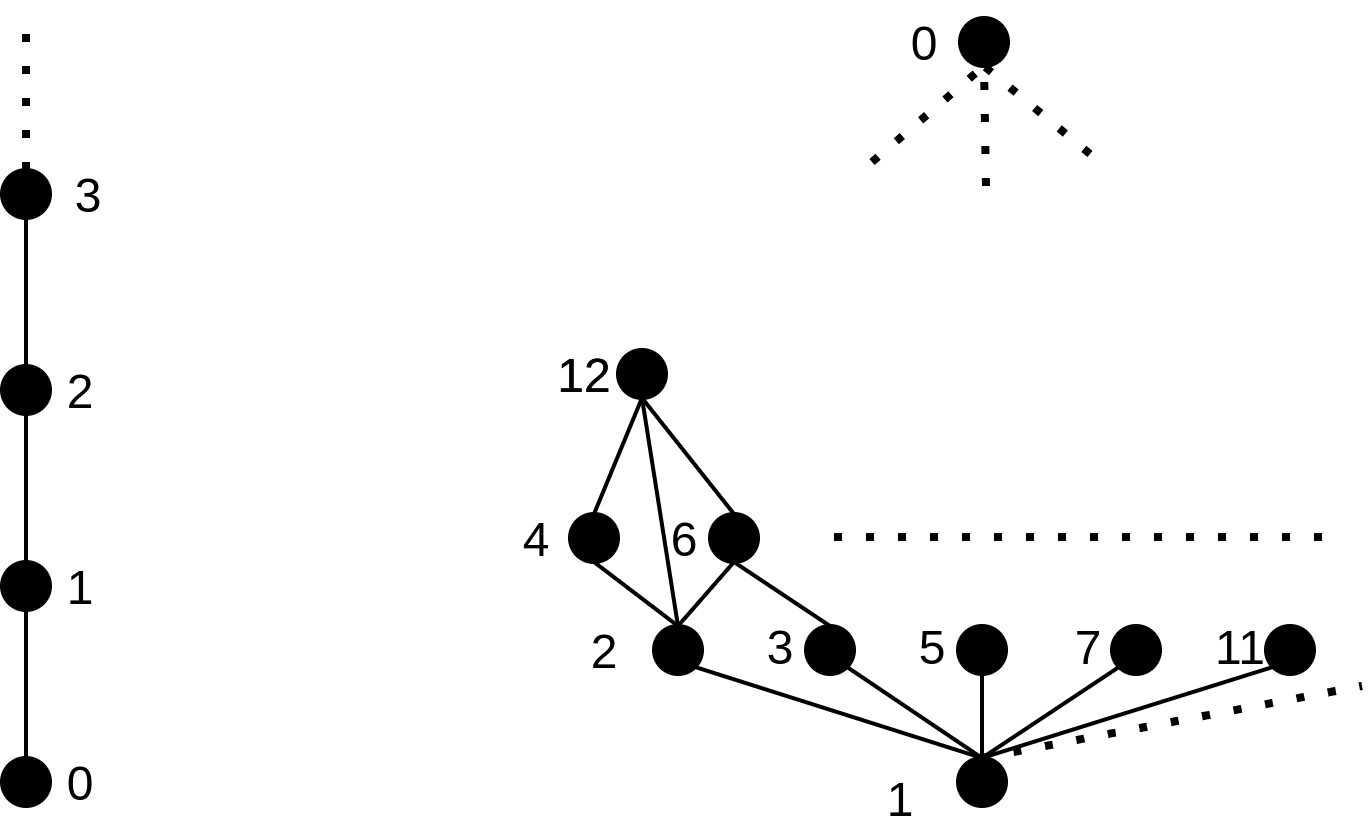
\includegraphics[width=0.5\textwidth]{images/reticolo2.png}
  \caption{Due relazioni d'ordine.}
  \label{figure:relazionireticoli}
\end{figure}

Nella Figura \ref{figure:relazionireticoli} si può vedere una rappresentazione 
(tramite reticoli, definiti a seguire) delle due relazioni d'ordine. 
La prima, quella totale, è rappresentata a destra: si può notare come sia 
``lineare'' a confronto della seconda, parziale, che è rappresentata a 
sinistra: quest'ultima infatti si dirama: alla base ha $1$, il numero che 
divide tutti gli altri; al primo ``strato'' ha tutti i numeri primi, 
il secondo i multipli dei multipli dei numeri primi (che saranno comunque collegati 
ai numeri primi, in quanto saranno divisibili anche per essi) e, commettendo 
un abuso che solitamente viene concesso, in cima vi è il numero $0$ che è divisibile 
da tutti gli altri, benché non sia divisibile per sé stesso. 

\subsubsection{Reticoli}
Un insieme $P$ con una relazione d'ordine (parziale) $\leq$, 
notato $(P, \leq)$ è detto insieme parzialmente ordinato 
o, in inglese, partially ordered set (\textit{poset}). 
L'insieme delle classi di equivalenza 
delle formule è un insieme parzialmente ordinato con delle peculiarità. 

Tra tutti i \textit{poset}, ci interessano quelli con alcune particolari proprietà 
strutturali, chiamati \textbf{reticoli}. 

\begin{figure}[!h]
  \centering 
  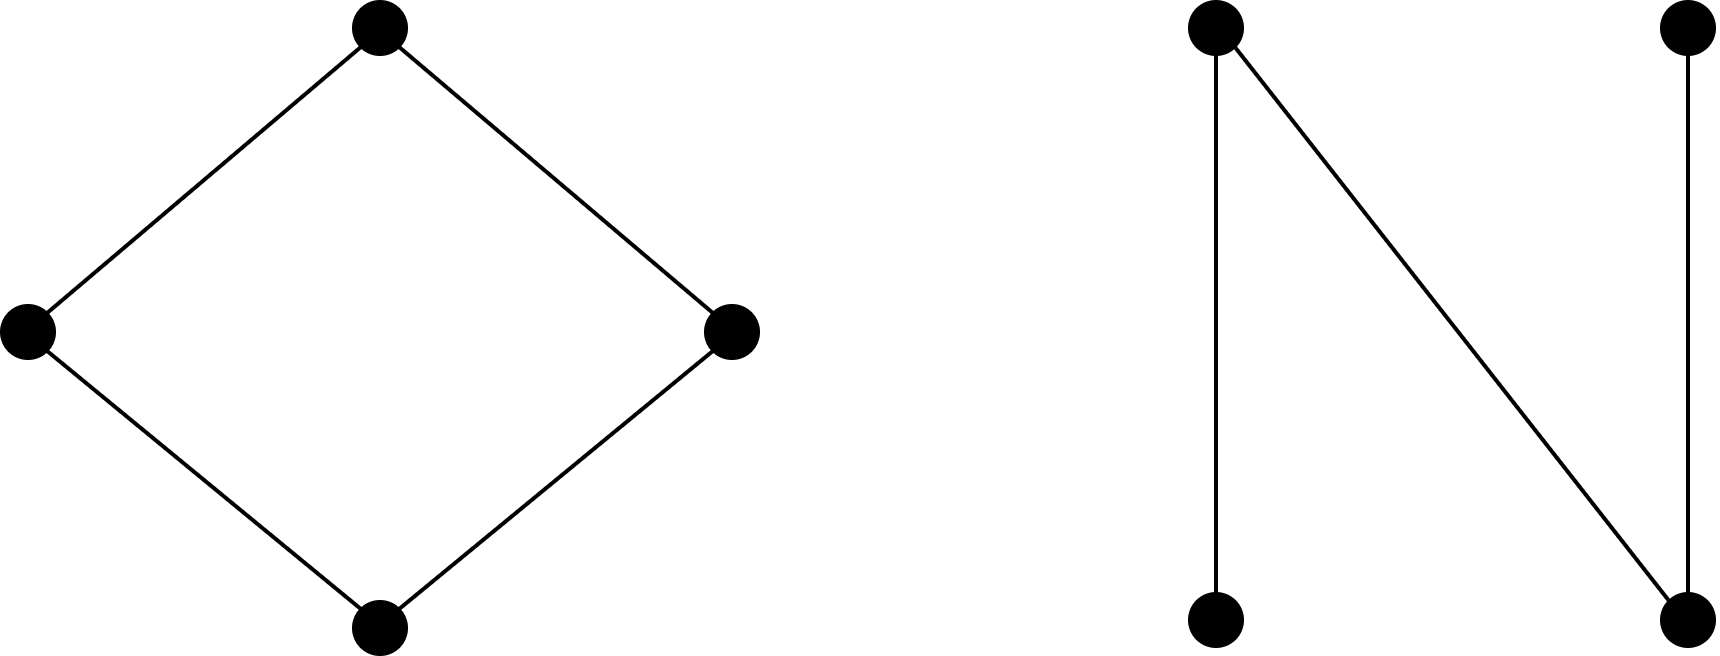
\includegraphics[width=0.5\textwidth]{images/reticolo.png}
  \caption{Due reticoli.}
  \label{figure:reticolo}
\end{figure}


La Figura \ref{figure:reticolo} riporta due immagini. 
Non entrambi sono reticoli: quello più a destra, infatti, non lo è. 
Cosa li distingue? La proprietà strutturale (più importante per i nostri 
scopi) che li divide, è che per quello più a sinistra, il reticolo, data 
ogni qualsiasi coppia di elementi possibile, si può sempre trovare 
quale dei due sia il minimo elemento che è più grande della coppia e il 
massimo elemento che è più piccolo della coppia. Questo non avviene nell'altro 
caso, infatti i due elementi ``in alto'', non hanno un minimo elemento 
più grande di loro, mentre i due elementi ``in basso'' non hanno un massimo 
elemento più piccolo di loro. In altre parole, non hanno 
\textbf{estremi inferiori} ed \textbf{estremi superiori}, che sono 
invece la proprietà fondamentale dei reticoli. 

Si definiscono quindi questi due concetti. 

\begin{defi}[Estremo inferiore]
  Dati due elementi $x, y$ appartenenti ad un insieme parzialmente ordinato $(P, \leq)$, si definisce 
  $$
  \inf(\{x,y\}) = \max\{z \in (P, \leq): z \leq x \text{ e } z \leq y\}
  $$
\end{defi}
e analogamente si definisce 
\begin{defi}[Estremo superiore]
  Dati due elementi $x, y$ appartenti ad un insieme parzialmente ordinato $(P, \leq)$, si definisce 
  $$
  \sup(\{x,y\}) = \min\{z \in (P, \leq): x \leq z \text{ e } y \leq z\}
  $$
\end{defi}
Si possono generalizzare $\inf()$ e $\sup()$ da un sottoinsieme $S \subseteq P$, con 
$P$ poset $(P, \leq)$:
\begin{align*}
  \inf(S) = \max\{z \in & (P, \leq): z \leq s\ \forall s \in S\} & \text{max dei minoranti di } S \\
  \sup(S) = \min\{z \in & (P, \leq): s \leq z\ \forall s \in S\} & \text{min dei maggioranti di } S \\
\end{align*}
A questo punto si può definire il minimo di un sottoinsieme (e analogamente il massimo), se esiste, come: 
\begin{align*}
  \min(S) := z \in S : z = \inf(S) &&
  \max(S) := z \in S : z = \sup(S)
\end{align*}
Si può ora definire formalmente un reticolo: 
\begin{defi}[Reticolo come poset]
Un reticolo è un insieme parzialmente ordinato $(R, \leq) : \forall x, y \in R$ esistono $\inf(\{x,y\})$ e $\sup(\{x,y\})$. 
\end{defi}

\noindent 
Dopo aver definito i reticoli, si definisce un'ulteriore struttura, necessaria per concludere l'argomento dell'Algebrizzazione della Logica Booleana. 

\subsection{Struttura Algebrica}
\begin{defi}
Dato un insieme $S$ e le operazioni $*_1, *_2, \cdots, *_n$ delle operazioni su $S$, allora $(S, *_1, *_2, \cdots, *_n)$ è una \textbf{struttura algebrica}.
\end{defi} 
\begin{defi}
  Visto come una struttura algebrica, un reticolo è $(R, \sqcup, \sqcap)$, con $\sqcup, \sqcap$ operazioni $\sqcup: R^2 \rightarrow R$ e $ \sqcap: R^2 \rightarrow R$, tale che le due operazioni siano commutative, associative e valga l'assorbimento.
\end{defi}
\begin{lem}
Ogni reticolo visto come insieme parzialmente ordinato è anche una struttura algebrica
$$
(R, \leq) \iff (R, \sqcup, \sqcap)
$$
\end{lem}
\begin{proof}
  ($\Longrightarrow$) con $R\equiv R,\ \forall a,b \in R$, siano:
  \begin{align*}
     a \sqcap b := \inf \{a,b\} && a \sqcup b := \sup \{a,b\}
  \end{align*}
  visto che si può verificare che per $\inf()$ e $\sup()$ valgono le proprietà di commutatività, assorbimento e associatività.
  
  ($\Longleftarrow$) con $R \equiv R$ definiamo $\forall a,b \in R$:
  \begin{align*}
    a \leq b \text{ sse } a = a \sqcap b &&
    b \leq a \text{ sse } a = a \sqcup b
  \end{align*}
  $(R, \leq)$ è quindi un poset, infatti si può verificare che $\leq$ è riflessiva, antisimmetrica e transitiva~(\ref{def:poset}). \\
  $(R, \leq)$ è anche un reticolo perché $\forall a,b \in R$ esiste $\inf$ e $\sup$: sia $c \leq a$ e $ c \leq b$
  \begin{align*}
    & c \leq a \text{ e } c \leq b \\
    \iff & c = c \sqcap a \text{ e } c = c \sqcap b & \text{per def. } \leq \\
    \iff & c = (c \sqcap b) \sqcap a \\
    \iff & c = c \sqcap (b \sqcap a) & \text{per associatività} \\
    \iff & c \leq b \sqcap a & \text{per def. } \leq \\
    \iff & c \leq \inf\{b, a\} & \text{per def. } \inf()
  \end{align*}
  Per il $\sup$ si ragiona in modo analogo. 
\end{proof}


\subsection{Definizione di Algebra Booleana}
A questo punto, siamo finalmente pronti per definire cosa sia l'Algebra Booleana.
\begin{defi}[Algebra Booleana]
L'Algebra Booleana è un sistema $(S, \sqcap, \sqcup, 0, 1, ()^c)$ di operazioni tali che $(S,\sqcup,\sqcap)$ sia un reticolo limitato, complementato, distributivo:
\begin{itemize}
  \item \textbf{limitato}: $\forall a \in S$:
    \begin{align*}
      & a \sqcup 0 = a & (a \geq 0) \\
      & a \sqcap 1 = a & (a \leq 1)
    \end{align*}
  \item \textbf{complementato}: $\forall a \in S$
    \begin{align*}
      a \sqcap a^c = 0 && a \sqcup a^c = 1
    \end{align*}
  \item \textbf{distributivo}: $\forall a,b, c \in S$:
    \begin{align*}
      a \sqcap (b \sqcup c) = (a \sqcap b) \sqcup (a \sqcap c) && a \sqcup (b \sqcap c) = (a \sqcup b) \sqcap ( a \sqcup c)
    \end{align*}
\end{itemize}
\end{defi}

Un esempio è il seguente: dato un insieme $A$ si consideri 
$(P(A), \cup, \cap, \emptyset, A, ()^c)$ e si ha 
$(P(A), \subseteq)$ tale che $A \subseteq B \iff A = A \cap B$. 

\paragraph{Esercizio}
Si dimostri che le seguenti sistemi siano un'algebra booleana:
\begin{itemize}
  \item $(F(A), \cup, \cap, \emptyset, A, ()^c)$ \\
    con $A$ un insieme infinito, e $F(A)$ l'insieme dei suoi sottoinsiemi finiti o complementi di insiemi finiti
  \item $(\{0,1\}, \min, \max, 0, 1, 1-\_)$
\end{itemize}

\subsubsection{Algebra di Lindenbaum}
L'algebra delle formule, chiamata anche \textbf{Algebra di 
Lindenbaum delle Formule}, è definita come 
$$
(\mathscr{F_L}/_{\equiv}, \land, \lor, \bot, \top, \neg)
$$
Dato che $\equiv$ è una congruenza, si possono definire le seguenti operazioni con $A,B \in \mathscr{F_L}$:
\begin{align*}
  [A]_{\equiv} \land [B]_{\equiv} & = [A \land B]_{\equiv} \\
  [A]_{\equiv} \lor [B]_{\equiv} & = [A \lor B]_{\equiv} \\
  [A]_{\equiv} \rightarrow [B]_{\equiv} & = [A \rightarrow B]_{\equiv} \\
  \neg [A]_{\equiv} & = [\neg A]_{\equiv} \\
  [\top]_{\equiv} & = \text{ tautologie} \\
  [\bot]_{\equiv} & = \text{ contraddizioni} \\
\end{align*}
La cardinalità dell'insieme delle classi di equivalenza scrivibili con $n$ variabili è:
$$
|\mathscr{F_L}^{(n)}/_\equiv| = 2 ^ {2^n} = |\{F: \{0,1\}^n \rightarrow \{0,1\}\}| = |\mathscr{P}(\{1,\cdots,2^n\})|
$$

\subsection{Funzioni Termine}
Al fine di arrivare ad un discorso completo sulle Forme Normali, si continua a ragionare sulle classi d'equivalenza delle formule e la loro struttura, ora da un punto di vista che sembra essere diverso ma che in conclusione si riunirà con quanto detto precedentemente. 

Si rifletta sul significato di 
\begin{align}
\label{fun:formula-computazionale}
\models F \iff \forall \mathcal{v}: \mathscr{L} \rightarrow \{0,1\},\ \mathcal{v}(F) = 1
\end{align}
in termini ``computazionali'' significa \textit{tenere fermo} l'argomento ($F$) e far cambiare le funzioni. Sarebbe comodo scambiare i ruoli: la formula si comporta come una funzione che prende come argomenti gli assegnamenti.

Siano $A \in \mathscr{F_L}$ una formula e $n \in \mathbb{N}$. Le lettere proposizionali che occorrono in $A$ si indicano con
$$
Var(A) \subseteq \mathscr{L} \subseteq \{p_1, p_2, \cdots, p_n\}
$$
Sia ora $\hat{A}$ una \textbf{funzione termine} $\hat{A} : \{0,1\}^n \rightarrow \{0,1\}$ tale che:
$$
\forall \mathcal{v}:\mathscr{L} \rightarrow \{0,1\},\ \hat{A}(\mathcal{v}(p_1), \mathcal{v}(p_2), \cdots, \mathcal{v}(p_n)) = \widetilde{\mathcal{v}}(A)
$$

\begin{defi}[Funziona Termine]
Definizione di $\hat A : \{0,1\}^n \rightarrow \{0,1\}$ induttiva su $A$:
\begin{itemize}
  \item \textbf{base}: Se $ A = p_i$, con $p_i \in \{p_1, p_2, \cdots, p_n\}$ un letterale:
  $$\hat A := \hat{p_i} : \{0,1\}^n \rightarrow \{0,1\}$$
  con $\hat{p_i}(t_1, \cdots, t_n) = t_i$, l'$i$-esima proiezione. 
  Quindi $\forall \mathcal{v}: \mathscr{L} \rightarrow \{0,1\}$ si verifica che: 
  $$
  \hat{A} = \hat{p_i}(\mathcal{v}(p_1), \cdots, \mathcal{v}(p_n)) = \mathcal{v}(p_i) = \widetilde{\mathcal{v}}(p_i) = \widetilde{\mathcal{v}}(A)
  $$
\item \textbf{passo}: $\forall (t_1, \cdots, t_n) \in \{0,1\}^n$
  \begin{itemize}
    \item Se $A = \neg B$: $\hat{A}(t_1, \cdots, t_n) =  1 - \hat{B}(t_1, \cdots, t_n)$
    \item Se $A = B \land C$: $\hat{A}(t_1, \cdots, t_n) = \min \{\hat{B}(t_1, \cdots, t_n),\ \hat{C}(t_1, \cdots, t_n)\}$
    \item Se $A = B \lor C$: $\hat{A}(t_1, \cdots, t_n) = \max \{\hat{B}(t_1, \cdots, t_n),\ \hat{C}(t_1, \cdots, t_n)\}$
    \item Se $A = B \rightarrow C$: $\hat{A}(t_1, \cdots, t_n) = \max \{1 - \hat{B}(t_1, \cdots, t_n),\ \hat{C}(t_1, \cdots, t_n)\}$
  \end{itemize}
\end{itemize}
\end{defi}
\noindent
Ora si possono vedere come \textit{funzioni termine} la riflessione iniziale~(\ref{fun:formula-computazionale}): 
$$
\models F \iff \hat{F}(t_1, \cdots, t_n) = 1,\ \forall (t_1, \cdots, t_n)
$$
e l'equivalenza logica: 
$$
[F]_{\equiv} = [G]_{\equiv} \iff F \equiv G \iff \hat{F}(t_1, \cdots, t_n) = \hat{G}(t_1, \cdots, t_n),\ \forall t_i \in \{0,1\}^n
$$
Allo stesso modo si può dare una definizione diversa di Algebra Booleana, \textit{isomorfa} all'Algebra di Lindenbaum.
\begin{defi}[Algebra Booleana su Funzioni Termine sui primi $n$ termini]
$$
\hat{\mathscr{F}}_\mathscr{L}^{(n)} = (\{\hat{A}: \{0,1\}^n \rightarrow \{0,1\}, A \in \mathscr{F_L}\}, \land, \lor, \neg, \bot, \top) 
$$
dove i significati degli operatori sono quelli espressi nella definizione di funzioni termine. 
\end{defi}

\subsection{Teorema di Completezza Funzionale}
Concentriamoci sull'algebra $\hat{\mathscr{F}}_\mathscr{L}^{(n)}$ appena espressa e una $Funz^{(n)}$ definita come:
$$
Funz^{(n)} = (\{f: \{0,1\}^{(n)} \rightarrow \{0,1\}\}, \land, \lor, \neg, \bot, \top)
$$
Che rapporto sussiste tra le due Algebre?
Per ogni $n \in \mathbb{N}$, la prima ha come universo l'insieme di tutte le Funzioni Termine per ogni formula $A \in \mathscr{F_L}$, mentre la seconda ha come universo tutte le funzioni $f: \{0,1\}^n \rightarrow \{0,1\}$. \\
Sicuramente, data la restrizione, si può affermare che:
$$
\hat{\mathscr{F}}_\mathscr{L}^{(n)} \subseteq Funz^{(n)}
$$
Si dimostra, ora, che vale anche:
$$
\hat{\mathscr{F}}_\mathscr{L}^{(n)} \supseteq Funz^{(n)}
$$
Questo fatto prende il nome di \textbf{Teorema di Completezza Funzionale}. 
A parole, ciò che afferma è che ogni funzione $f: \{0,1\}^n \rightarrow \{0,1\}$ è esprimibile come una formula $F \in \mathscr{F_L}$. \\
Chiaramente, se dimostrato, vuol dire che le due algebre sono in realtà \textit{isomorfe}. 
\begin{teo}[di Completezza Funzionale]
$$
  \mathscr{\hat{F}_L}^{(n)} \supseteq Funz^{(n)},\ \forall n \in \mathbb{N}
$$
\end{teo}

La dimostrazione consiste nel fornire per ogni $n \in \mathbb{N}$ e ogni funzione $f: \{0,1\}^{n} \rightarrow \{0,1\}$ una formula \textit{costruibile} $F \in \mathscr{F_L}^{(n)} : f = \hat F$. 
\begin{proof}
Sia $f: \{0,1\}^{n} \rightarrow \{0,1\}$ una funzione, la cui cardinalità del dominio è $2^{n}$. Per ogni combinazione degli $n$ argomenti $(a_{i_1}, a_{i_2}, \cdots, a_{i_n})$ esiste un valore $b_i \in \{0,1\}$ associato:
\begin{align}
  f :=
  \begin{cases}
    (a_{1_1}, a_{1_2}, \cdots, a_{1_j}, \cdots, a_{1_n}) & \longrightarrow b_1 \\
    (a_{2_1}, a_{2_2}, \cdots, a_{2_j}, \cdots, a_{2_n}) & \longrightarrow b_2 \\
    ~~~~~~~~~~~~~~~     \vdots           & ~~~~~~~~ \vdots \\
    (a_{i_1}, a_{i_2}, \cdots, a_{i_j}, \cdots, a_{i_n}) & \longrightarrow b_i \\
    ~~~~~~~~~~~~~~~     \vdots           & ~~~~~~~~ \vdots \\
    (a_{(2^n)_1}, a_{(2^n)_2}, \cdots, a_{(2^n)_j}, \cdots, a_{(2^n)_n}) & \longrightarrow b_{(2^n)}
  \end{cases}
\end{align}
Costruiamo una formula $F \in \mathscr{F_L}$ in modo tale che $ \hat{F} = f$.
\begin{itemize}
  \item se $f(t_1, \cdots, t_n) = 0$ per ogni $(t_1, \cdots, t_n)$: $F = \bot$
  \item altrimenti sia $I \subseteq \{1, 2, \cdots, 2^{n}\}$ tale che:
  $$
  i \in I \iff b_i = 1
  $$
  (intuitivamente, $I$ contiene i numeri delle ``righe'' della tabella di verità della funzione $f$ in cui l'immagine è il numero $1$). \\
  Per ogni $i \in I$ si considera la $i$-esima tupla $(a_{i_1}, a_{i_2}, \cdots, a_{i_n})$ di argomenti di $f$. \\
  Per ogni $j \in \{1, \cdots, n\}$ si definisce:
  \begin{align*}
  A_{ij} =
  \begin{cases}
    p_j & \text{se } a_{ij} = 1 \\
    \neg p_j & \text{se } a_{ij} = 0
  \end{cases} &&
  \text{con } A_{ij} \in \mathscr{F_L}^{(n)}
  \end{align*}
  Si pone $F = \bigvee\limits_{i \in I}\bigwedge\limits_{j \in n} A_{ij}$
  
  Si mostra che $\hat{F} = f$, ovvero che per ogni riga $i \in I$:
  $$
  {[ \bigwedge\limits_ {j = 1}^{n} \hat{A}_{ij}(t_1, \cdots, t_n) ]} = 1
  \iff (t_1, \cdots, t_n) = (a_{i_1}, \cdots, a_{i_n})
  $$
  Infatti
  \begin{itemize}
  \item se $(t_1, \cdots, t_n) = (a_{i_1}, \cdots, a_{i_n})$, $\forall j \leq  n$:
    \begin{align*}
      \hat A_{ij}(t_1, \cdots, t_n) = t_j =
      \begin{cases*}
        \mathcal{v}(p_j) = a_{i_j} \\
        \mathcal{v}(\neg p_j) = 1 - a_{i_j}
      \end{cases*}
      &
      \begin{rcases*}
        \text{ se } a_{i_j} = 1 \\
        \text{ se } a_{i_j} = 0
      \end{rcases*} = 1
    \end{align*}
  \item se $(t_1, \cdots, t_n) \neq (a_{i_1}, \cdots, a_{i_n})$, $\exists t_j \neq a_{i_j}$:
    \begin{align*}
      \hat A_{ij}(t_1, \cdots, t_n) = t_j =
      \begin{cases*}
        \mathcal{v}(p_j) = a_{i_j} \\
        \mathcal{v}(\neg p_j) = 1 - a_{i_j}
      \end{cases*}
      &
      \begin{rcases*}
        \text{ se } a_{i_j} = 0 \\
        \text{ se } a_{i_j} = 1
      \end{rcases*} = 0
    \end{align*}
  \end{itemize}
  Quindi $(A_{i_1} \land A_{i_2} \land \cdots \land A_{i_n})$ può essere resa vera solo da un assegnamento. In definitiva, 
  $$
  \hat{F} = \bigvee\limits_{i\in I}\bigwedge\limits_{j}^n \hat A_{i_j}(t_1, \cdots, t_n) = 1 \iff (t_1, \cdots, t_n) \text{ è la riga } i \text{-esima, e } i \in I
  $$
  Quindi $\hat F = f$.  
\end{itemize}
\end{proof}

\subsubsection{Considerazioni sul Teorema di Completezza Funzionale}
Per come è stato provato il Teorema di Completezza Funzionale, la funzione termine si può anche esprimere come: 
$$
G = \bigwedge\limits_{i \in J} \bigvee_{j = 1}^{n} B_{ij}
$$
con
\begin{align*}
  J \subseteq \{0, \cdots, 2^n-1\} &&
  i \in J \iff b_j = 0 &&
  B_{ij} =
  \begin{cases}
    \neg p_j & a_{ij} = 1 \\
    p_j & a_{ij} = 0 \\
  \end{cases}
\end{align*}
Si ha, quindi, che $\hat{F} = f = \hat{G}$\footnote{Ciò che è stato fatto è esattamente uguale alla costruzione dei minterm e maxterm per una data tavola di verità.}, il che è una dimostrazione che una qualsiasi formula può essere messa in una \textbf{forma normale} perché $\hat{\mathscr{F}}_\mathscr{L}^{(n)} = Funz^{(n)}$.

Sebbene il Teorema possa sembrare banale, in quanto la sua dimostrazione è
semplice, il suo contenuto non è nullo né scontato. Un esempio di mancanza 
funzionale è già presente nella Logica Proposizionale stessa, nonostante 
la dimostrazione precedente, rimuovendo il vincolo su $n$ e definendo
$$
Funz^{\omega} := \{f:\{0,1\}^{\omega} \rightarrow \{0,1\}\}
$$
con $\omega = |\mathbb{N}|$, in altre parole l'insieme di tutte le successioni 
infinite di valori $\{0,1\}$. Se valesse il Teorema di Completezza Funzionale 
anche in questo caso, si dovrebbe poter affermare che tale insieme 
è incluso nelle classi di equivalenza scritte nelle classi di equivalenza 
delle formule scritte con $\omega$ variabili: 
$$
Funz^{\omega} \subseteq \hat{\mathscr{F}}_\mathscr{L}^{\omega} = \mathscr{F_L}^{\omega}/_\equiv
$$
Ma in realtà
$$
|Funz^{\omega}| = |\mathbb{R}| \geq |\mathbb{N}| = |\mathscr{F_L}^{\omega}/_\equiv|
$$
e pertanto non è valido. 

\paragraph{Forme Normali Canoniche}
Le forme normali che abbiamo trovato non sono desiderabili per gli scopi 
futuri, in quanto sono molto prolisse: ognuno degli $A_{ij}$ menziona 
tutte le lettere proposizionali $p_1, \cdots, p_n$ (analogamente per le 
forme congiuntive) ed è infatti chiamata Forma Normale Disgiuntiva (or di and) \textbf{Canonica} o \textbf{Completa}. \\
Si noti la prolissità nel costruire una $F \in \mathscr{F_L}$ t.c. $\hat F = f : \{0, 1\}^3 \rightarrow \{0, 1\}$ con: 
$$
f(t_1, t_2, t_3) = t_1 ~~~ \forall (t_1, t_2, t_3)
$$
È chiaro che la formula più ``corta'' è $F = t_1$, ma con la forma 
canonica si rappresenta come:
$$
F = (p_1 \land \neg p_2 \land \neg p_3) \lor (p_1 \land \neg p_2 \land p_3) \lor (p_1 \land p_2 \land \neg p_3) \lor (p_1 \land p_2 \land p_3)
$$

\paragraph{Insieme funzionalmente completo di connettivi}
C'è un'altra nozione, legata alla Completezza Funzionale, che è molto interessante, 
ossia la nozione di \textit{insieme funzionalmente completo di connettivi}. 
\begin{defi}[Insieme funzionalmente completo di connettivi]
Un insieme 
  $$
  C \subseteq \{\land, \lor, \rightarrow, \neg, \leftrightarrow, \bot, \top\}
  $$
è definito \textit{funzionalmente completo} se per ogni $F \in \mathscr{F_L}$ esiste una $G \in \mathscr{F_L}$ scritta usando solo i connettivi in $C$ tale che $F \equiv G$ e $\hat{F} = \hat{G}$, ossia $[F]_{\equiv} = [G]_{\equiv}$. 
\end{defi}

Un insieme di connettivi funzionalmente 
completo è dato dal Teorema di Completezza Funzionale stesso, ossia 
$C = \{\land, \lor, \neg\}$. Si può mostrare facilmente che 
anche $\{\neg, \land\}$ e $\{\neg, \lor\}$ sono completi (in quanto, grazie alle 
leggi di De Morgan, $(A \lor B) = \neg (\neg A \land \neg B)$). Questi non 
sono gli unici insiemi funzionalmente completi: 
$\{\neg, \rightarrow\}$ (in quanto $(A \land B) \equiv \neg (A \rightarrow \neg B)$ 
e $(A \lor B) \equiv ((\neg A) \rightarrow B)$ 
e $\{\rightarrow, \bot\}$. In particolare, un insieme composto da un 
solo connettivo, il \texttt{nand}, è anch'esso funzionalmente completo, 
in quanto ogni altro connettivo è ricostruibile utilizzando solo 
$$
A \barwedge B = \neg (A \land B)
$$
infatti $\neg A \equiv A \barwedge A$ e, ovviamente, $A \land B \equiv \neg ( A \barwedge B)$ 
per definizione. 

\section{Forme Normali}
Dopo averle introdotte col Teorema di Completezza Funzionale, possiamo 
passare ad un esame più approfondito delle Forme Normali.
Le Forme Normali Congiuntive e Disgiuntive Canoniche sono 
esageratamente prolisse. Sarebbe utile conservare l'idea delle Forme Normali 
con formule più succinte. 

\subsection{Forma Normale Negata}
Una terza forma normale, chiamata \textbf{Negation 
Normal Form} (NNF) che, per definizione, è l'insieme delle formule 
che rispettano le seguenti proprietà: 
\begin{itemize}
  \item non contiene $\rightarrow$ 
  \item $\neg$ occorre solo applicato a lettere proposizionali
\end{itemize}
quindi, per esempio 
\begin{align*}
p_1 \land \neg(p_2 \lor p_3) \notin NNF \\
p_1 \land (\neg p_2 \lor \neg p_3) \in NNF
\end{align*}

\begin{defi}[Sottoformula]
$G$ è sottoformula di $F$ sse $G$ occorre in ogni $\mathscr{L}$-costruzione di $F$ e si indica con $G \preccurlyeq F$
\end{defi}

\begin{lem}
Ogni formula $F \in \mathscr{F_L}$ è equivalente a una $F^{N} \in NNF$. 
\end{lem}
\begin{proof}
Per provare il lemma, descriviamo come trasformare $F$ in $F^{N}$ in un numero 
finito di passi, dove ogni passo produce una formula equivalente alla precedente. 
Per ottenere la sequenza si applica ad ogni passo una delle seguenti 
trasformazioni a $G \preccurlyeq F$:

\begin{enumerate}
  \item $C \rightarrow D \leadsto (\neg C) \lor D$
  \item $\neg \neg C \leadsto C$
  \item $\neg(C \lor D) \leadsto \neg C \land \neg D$
  \item $\neg (C \land D) \leadsto \neg C \lor \neg D$
\end{enumerate}

Un'osservazione preliminare su questo algoritmo è che si può mostrare che applicando 
le quattro regole in un ordine qualsiasi si ottiene sempre $F^{N} \in NNF$. 
Si mostrerà che partendo da $(1)$ e applicando le altre trasformazioni si possa 
arrivare a $F^{N}$: sia data $F \in \mathscr{F_L}$. In un numero finito di applicazioni 
di $(1)$ si ottiene una $F'$ in IFNF (Implication-Free Normal Form), equivalente 
a $F$. 

Si introduce una misura di \textit{distanza}: si definisce 
$i(E)$ come il numero di connettivi $\rightarrow$ nella formula $E$. 
Si ha, quindi, 
che $E \in IFNF \iff i(E) = 0$. Inoltre, se $E \notin IFNF$, allora 
$E'$ ottenuta applicando $(1)$ su $E$ deve avere $i(E) > i(E')$.\\
È chiaro che $F \equiv F'$ poiché l'applicazione di $(1)$ è semplicemente 
l'applicazione di una equivalenza eseguita grazie al Teorema di Sostituzione. 
Quindi, in un certo numero di passi  si ha
$$ 
F = F_0 \equiv \cdots \equiv F' (\in IFNF) \equiv F_i \equiv \cdots \equiv F_n (\in NNF)
$$
e si nota che le applicazioni di $(2)$, $(3)$ e $(4)$ trattano tutte equivalenze logiche. Ciò che bisogna dimostrare è che la sequenza di trasformazioni termini, ossia l'algoritmo non è infinito ($n \in \mathbb{N}$).

Per dimostrare che l'algoritmo termina, siano ora $A,E \in \mathscr{F_L}$ e si definisce $\ell(A) = $ ``n° di occorrenze di connettivi in $A$''.
Definiamo quindi $m(E)$ come la somma del numero di connettivi presenti nelle sottoformule $\neg A$ di $E$: 
$$
m(E) = \sum_{\neg A \preccurlyeq E} \ell(A)
$$
Si noti che 
$$
m(E) = 0 \iff E \in NNF
$$
Infatti:
\begin{itemize}
  \item  se $E \in NNF$:
    \begin{align*}
      & \forall \neg A \preccurlyeq E,\ A \in \mathscr{L} & \text{per def. } NNF\\
      \iff & \forall \neg A \preccurlyeq E,\ \ell(A) = 0 \\
      \iff & m(E) = 0
    \end{align*}
  \item se $m(E) = 0$:
    $$
    \sum_{\neg A \preccurlyeq E} \ell(A) = 0 \iff \forall \neg A \preccurlyeq E,\ \ell(A) = 0 \iff \forall \neg A \preccurlyeq E,\ A \in \mathscr{L}
    $$ 
\end{itemize}
In un passaggio eseguito con una delle $(2), (3), (4)$ generando 
$$
E \leadsto E'
$$
si ha che $m(E) > m(E')$. Se si riesce a dimostrare quest'ultima affermazione, 
allora si dimostra automaticamente che il procedimento termina in un numero 
finito di passi. 
\paragraph{(2) $\neg \neg C \leadsto C$}: In questo caso
\begin{align*}
  \begin{cases}
        m(\neg \neg C) & = \ell(\neg C) + m(\neg C)
                         = \ell(C) + 1 + \ell(C) + m(C) \\
                       & = 1 + 2 \cdot \ell(C) + m(C) \\
        m(C)
  \end{cases}
\end{align*}
$$
  \implies m(\neg \neg C) > m(C)
$$

\paragraph{(3) $\neg (C \lor D) \leadsto \neg C \land \neg D$}: In questo caso
\begin{align*}
  \begin{cases}
    m(\neg (C \lor D)) & = \ell(C \lor D) + m(C) + m(D) \\
                       & = \ell(C) + \ell(D) + m(C) + m(D) + 1 \\
    m(\neg C \land \neg D) 
                       & = \ell(C) + \ell(D) + m(C) + m(D)
  \end{cases}
\end{align*}
$$
  \implies m(\neg (C \lor D)) > m(\neg C \land \neg D)
$$
Analogamente per $(4)$.

Data una formula $F \in \mathscr{F_L}$, si può costruire una successione 
finita 
$$ 
F = F_0 \equiv \cdots \equiv F' (\in IFNF) \equiv F_i \equiv \cdots \equiv F_n (\in NNF)
$$
e ovviamente $F \equiv F_n$, per un qualche $n \in \mathbb{N}$. 
\end{proof}

\subsection{Forma Normale Congiuntiva e Disgiuntiva}
Le CNF o FNC, Forme Normali Congiuntive, sono un sovrainsieme delle CNF \textit{complete} o canoniche.
\begin{defi}[Letterale]
Un \textit{letterale} è una formula nella forma $p$ o $\neg p$ per qualche lettera proposizionale $p$ (i.e., o è una lettera proposizionale o è la sua negata).
La definizione di \textbf{letterale opposto} a uno dato è, dato $A$ letterale, l'opposto di $A$:
$$
\bar{A} = 
\begin{cases}
  \neg p & \text{se } A = p \\
  p & \text{se } A = \neg p
\end{cases}
$$
\end{defi}
\begin{defi}[Clausola]
Una \textit{clausola} è una disgiunzione di un numero finito $k$ di letterali:
$$
\ell_1 \lor \ell_2 \cdots \lor \ell_k
$$
dove ogni $\ell_i$ è un letterale. 
\end{defi}
\begin{defi}[CNF o FNC]
Una \textbf{forma normale congiuntiva} è una congiunzione di un numero finito $h$ di 
clausole: 
$$
C_1 \land C_2 \land \cdots \land C_h
$$
dove ogni $C_j$ è una clausola. 
\end{defi}
\begin{defi}[Clausola vuota]
Una \textbf{clausola vuota} $\qedsymbol$ è definita come la disgiunzione 
di zero letterali. 
\end{defi}

Questo concetto è importante e non va confuso col concetto 
di \textbf{CNF vuota} $\emptyset$, definita come la congiunzione di zero clausole. 
Prendendo una sequenza di letterali e formule
\begin{align*}
F_0 & = \qedsymbol \\
F_1 & = \ell_1 \\
F_2 & = \ell_1 \lor \ell_2 \\
F_3 & = \ell_1 \lor \ell_2 \lor \ell_3 \\
\vdots \\
F_i & = \ell_1 \lor \ell_2 \lor \ell_3 \lor \cdots \lor \ell_i
\end{align*}
possiamo notare che ogni assegnamento che soddisfa una formula $F_i$, soddisfa anche quella successiva $F_{i+1}$. Per questo $F_i \rightarrow F_{i+1}$ è una tautologia. \\
Seguendo questa definizione la clausola vuota è insoddisfacibile e pertanto è $\qedsymbol \equiv \bot$.

Per l'insieme di CNF vuote, si ha 
\begin{align*}
& \emptyset \\
& C_1 \\
& C_1 \land C_2 \\
& C_1 \land C_2 \land C_3\\
& \vdots \\
& C_1 \land C_2 \land C_3 \land C_4
\end{align*}
qui, al contrario, ogni assegnamento che soddisfa una clausola $C_i$, soddisfa anche la precedente $C_{i-1}$. \\
Seguendo questa definizione la CNF vuota è soddisfacibile ed è, in realtà, soddisfatta da ogni assegnamento: $\emptyset \equiv \top$. 

\begin{defi}[DNF o FND]
Una \textit{forma normale disgiuntiva} è una disgiunzione di un numero finito $n$ di formule:
$$
D_1 \lor D_2 \lor \cdots \lor D_n
$$
dove ogni $D_i$ è una congiunzione chiamata \textbf{co-clausola} di un numero finito $v$ di letterali:
$$
\ell_1 \land \ell_2 \land \cdots \land \ell_v
$$
\end{defi}

DNF si tratta, quindi, di una struttura duale rispetto alle CNF.
Si noti la terminologia speciale per le CNF: questa terminologia è riservata alle CNF in quanto la dualità tra CNF e DNF verrà spezzata. 

\begin{lem}
Ogni formula $F \in \mathscr{F_L}$ è logicamente equivalente a una formula $F^c \in CNF$ 
e a una formula $F^d \in DNF$.
\end{lem}

Questo è già stato dimostrato grazie al teorema di completezza funzionale, che tuttavia utilizzava le CNF e DNF complete. 
\begin{proof}[esistenza DNF/CNF]
Per induzione strutturale su $F$:
\begin{itemize}
  \item \textbf{base}: se $F = p$ con $p \in \mathscr{L}$ allora $p = p^c = p^d$.
  \item \textbf{passo}:
    \begin{itemize}
      \item se $F = \neg G$, per ipotesi induttiva si ha $G^c \equiv G$ e $G^d \equiv G$. 
        Allora, se
        \begin{align*}
           G = C_1 \land C_2 \land \cdots \land C_h &&
          \text{dove ogni } C_i = \ell_{i_1} \lor \cdots \lor \ell_{i_{k_i}}
        \end{align*}
        si ha che:
        \begin{align*}
          \neg G \equiv \neg (G^c) & \equiv \neg (C_1 \land \cdots \land C_h) \\
                   & \equiv \neg C_1 \lor \neg C_2 \lor \cdots \lor \neg C_h := (\neg G)^d & \text{per DeMorgan}
        \end{align*}
        \begin{align*}
          \text{dove ogni } \neg C_i & \equiv \neg (\ell_1 \land \ell_2 \land \cdots \land \ell_v) \\
                               & \equiv \neg \ell_{i_1} \land \cdots \land \neg \ell_{i_{k_i}} & \text{per DeMorgan} \\
                               & \equiv \bar \ell_{i_1} \land \cdots \land \bar \ell_{i_{k_i}} & \neg \ell_{i_j} \text{ è } \equiv \text{ a un letterale opposto} \\
          \implies (\neg G)^d \in DNF 
        \end{align*}
        e similmente:
        \begin{align*}
          \neg G \equiv \neg (G^d) & \equiv \neg (D_1 \lor \cdots \lor D_n) \\
                   & \equiv \neg D_1 \land \neg D_2 \land \cdots \land \neg D_n := (\neg G)^c & \text{per DeMorgan}
        \end{align*}
        \begin{align*}
          \text{con } \neg D_i & \equiv \neg (\ell_{i_1} \land \cdots \land \ell_{i_{k_i}}) \\
                               & \equiv \neg \ell_{i_1} \land \cdots \land \neg \ell_{i_{v_i}} & \text{per DeMorgan} \\
                               & \equiv \bar \ell_{i_1} \land \cdots \bar \neg \ell_{i_{v_i}} & \neg \ell_{i_j} \text{ è } \equiv \text{ a un letterale opposto} \\
          \implies (\neg G)^c \in CNF 
        \end{align*}
        Quindi esistono sia $F^d := (\neg G)^d \equiv \neg (G^c)$ che $F^c := (\neg G)^c \equiv \neg (G^d)$. 
      \item se $F = (G \land H)$, per ipotesi induttiva si ha:
        \begin{align*}
           G^c \equiv G && G^d \equiv G \\
           H^c \equiv H && H^d \equiv H
        \end{align*}
        Si definisce, allora
        \begin{itemize}
          \item $F \equiv F^c$ \\
                con $F^c := (G^c \land H^c)$ e, banalmente $(G^c \land H^c) \in CNF$
          \item $F^d$:
            \begin{align*}
              F & \equiv (G^d \land H^d) \\ 
                & \equiv (G_1 \lor \cdots \lor G_u) \land (H_1 \lor \cdots \lor H_v) \\
                & \equiv \bigvee\limits_{i,j}(G_i \land H_j) & \text{per Distributività Generalizzata}~(\ref{def:distributibilita-generalizzata})
            \end{align*}
            Ma visto che $C_i$ e $H_j$ sono \textit{co-clausole}, anche $(G_i \land H_j)$ lo è.
            $$
            \implies F^d := \bigvee\limits_{i=1}^u \bigvee\limits_{j=1}^v (G_i \land H_i) \in DNF
            $$
        \end{itemize}
      \item se $F = (G \lor H)$, per ipotesi induttiva si ha:
        \begin{align*}
          G^c \equiv G && G^d \equiv G \\
          H^c \equiv H && H^d \equiv H
        \end{align*}
        Si definisce, allora
        \begin{itemize}
          \item $F \equiv F^d$ \\
                con $F^d := (G^d \lor H^d)$ e, banalmente $(G^d \lor H^d) \in DNF$
          \item $F^c$:
            \begin{align*}
              F & \equiv (G^c \lor H^c) \\ 
                & \equiv (G_1 \land \cdots \land G_u) \lor (H_1 \land \cdots \land H_v) \\
                & \equiv \bigwedge\limits_{i,j}(G_i \lor H_j) & \text{per Distributività Generalizzata}~(\ref{def:distributibilita-generalizzata})
            \end{align*}
            Ma visto che $C_i$ e $H_j$ sono \textit{clausole}, anche $(G_i \lor H_j)$ lo è.
            $$
            \implies F^c := \bigwedge\limits_{i=1}^u \bigwedge\limits_{j=1}^v (G_i \lor H_i) \in CNF
            $$generalizzata
        \end{itemize}       
      \item se $F = (G \rightarrow H)$, ci si comporta analogamente contando che $F \equiv (\neg G \lor H)$      
    \end{itemize}
\end{itemize}
\end{proof}

Si nota, tuttavia, che muoversi tra DNF e CNF con la distributività generalizzata causa un notevole allungamento delle formule. Per esempio:
\begin{align*}
        \bigvee\limits_{i = 1}^{n} (p_i \land q_i) \equiv \bigwedge\limits_{i = 1}^{2^n}(\ell_{i_1} \lor \cdots \lor \ell_{i_n})
\end{align*}
quindi c'è una dilatazione esponenziale. Questo è un bel problema.


Ci sono algoritmi più intelligenti per generare da DNF delle formule CNF più corte? \\
Purtroppo no. 

\chapter{Complessità Computazionale e Deduzione Automatica}

In questo momento, per decidere se una formula $F \in \mathscr{F}_\mathscr{L}$ che menziona $n$ lettere proposizionali diverse sia soddisfacibile o meno, l'algoritmo che conosciamo computa la sua tabella di verità, analizzando quindi $2^n$ possibilità, ossia un numero esponenziale. 
qui
Cominciamo definendo cosa sia un problema di decisione:
\begin{defi}[Problema di Decisione]
Dato $\Sigma^*$ un insieme di tutte le \textit{parole} finite costruite coi simboli di $\Sigma$—un \textit{alfabeto} finito—e un \textit{Linguaggio} $L \subseteq \Sigma^*$, non necessariamente finito, il problema di decisione consiste nel verificare se una stringa finita $w$ appartenga o meno al Linguaggio $L$
\end{defi}

Ad esempio, fissato 
$$
\Sigma = \{\land, \lor, \neg, \rightarrow, (, ), p, |\}
$$
si possono definire alcuni problemi, per esempio
$$
\mathscr{F}_\mathscr{L} \subseteq \Sigma ^*
$$
dove il problema risiede nel capire se una certa formula di lunghezza finita
risiede in $\mathscr{F}_\mathscr{L}$ oppure no. 
Vi sono dei problemi principalmente di natura sintattica, come appunto $\mathscr{F}_\mathscr{L}$ 
ma anche $NNF$, $CNF$ e $DNF$. Vi sono problemi in cui la natura semantica 
è decisiva, per esempio $SAT$, dove 
$$
w \in \Sigma^* : w\in SAT \iff w \in \mathscr{F}_\mathscr{L} \land w \text{ è soddisfacibile}
$$
oppure $TAUTO$, dove una stringa finita appartiene a $TAUTO$ sse è una formula ed è una tautologia, ossia
$$
w \in \Sigma^* : w \in TAUTO \iff w \in \mathscr{F}_\mathscr{L} \land \models w
$$
e analogamente $UNSAT$, il problema di decidere se una certa formula è
insoddisfacibile.

\section{Complessità Computazionale}
\subsection{Efficienza}
Alcuni dei problemi elencati precedentemente possono essere risolti (decisi) 
in maniera efficiente, ossia data una \textit{parola} $w$ decidere se 
appartiene ad un certo linguaggio: esempi di soluzioni efficienti sono 
quelle che riguardano tutti i problemi sintattici, risolvibili in tempo 
al massimo quadratico e in realta anche lineare con alcune tecniche di parsing. 

I problemi che riguardano la semantica, invece, sono tipicamente più complessi
da risolvere e infatti, per quanto conosciamo fino ad ora, si possono risolvere 
solo (nel caso peggiore) con un analisi dell'intera tabella di verità della 
formula, quindi con un numero esponenziale di calcoli. \`E importante rimarcare 
nuovamente che benché sussista questa difficoltà, verificare che 
un singolo assegnamento verifichi la formula è invece un calcolo semplice 
che richiede un tempo decisamente più contenuto rispetto al problema di 
decidibilità.

Quindi, vi sono dei problemi decidibili efficientemente, 
dei problemi decidibili molto difficilmente e verificabili facilmente 
e dei problemi decidibili molto difficilmente e verificabili difficilmente; 
da qui parte una gerarchia di classi di complessità infinita, ma a noi interesseranno 
solo le prime due. 
 
Per essere più precisi, si fissa un modello astratto di computazione, che fornisca 
la nozione di \textit{passo elementare}, in modo da poter ragionare precisamente 
sull'efficienza dei problemi. 
Qualunque modello di computazione che costituisca un modello realistico 
di calcolatore, con associata una nozione di passo elementare per costruire 
algoritmi, classifica i problemi nello stesso modo. 

\begin{oss}[Tesi di Church-Turing]
  Ogni modello ragionevole di computazione è equivalente.
\end{oss}

Uno dei modelli di computazione è quello delle Macchine di Turing (MdT): un'idea 
della Macchina di Turing è immaginarla come una macchina che lavora su un 
nastro infinito in lettura e scrittura, mantenendo uno stato e operando su 
una singola porzione di nastro in lettura utilizzando un programma per 
muoversi tra gli stati e scrivere sul nastro. 

Si può passare ora alla definizione formale delle classi dei problemi: 
\begin{defi}[Classe $\mathbb{P}$]
  La classe dei problemi ``efficientemente decidibili'' è definita, con una 
  certa ideologia sottesa, come tutti quei problemi che possono essere 
  risolti in tempo polinomiale, ossia esiste una certa Macchina di Turing T 
  e un polinomio $p: \mathbb{N}\rightarrow \mathbb{N}$ per i quali per ogni 
  $w \in \Sigma^*$  la computazione della MdT sull'input $w$, 
  denotato $T(w)$ termina entro $p(||w||)$ passi e per ogni $w \in L$ si 
  ha che $T(w)$ accetta il problema e per ogni $w \notin L$  si ha 
  che $T(w)$ non accetta, ossia risolve il problema.
\end{defi}

\begin{defi}[Classe $\mathbb{NP}$]
  La classe dei problemi ``verificabili efficientemente'' è definita come 
  tutti quei problemi tali per cui esiste una Macchina di Turing deterministica 
  e due polinomi $p,q:\mathbb{N}\rightarrow \mathbb{N}$ tali che per ogni 
  $w \in \Sigma^*$ e ogni $z \in \Gamma^*$, ossia un \textbf{certificato}, 
  che si può immaginare prodotto da un oracolo, si ha 
  che $T(w,z)$ termina entro $p(||w||)$ passi e si ha che per ogni 
  $w \in L$ esiste $z \in \Gamma^*$ tale che $||z|| \leq q(||w||)$ (ossia 
  il certificato è sufficientemente corto) e $T(w,z)$ accetta e per ogni 
  $w \notin L$ si ha che per ogni possibile $z \in \Gamma^*$ sufficientemente corto
  $T(w,z)$ rifiuta, ossia ``valida'' il certificato.
\end{defi}

\begin{defi}[Riducibilità]
        Un problema $L_1 \subseteq \Sigma^*$ è \textbf{riducibile in tempo polinomiale} 
        a un altro problema $L_2 \subseteq \Gamma^*$ se e solo se esistono
        una Macchina di Turing $T_{{L_1}, {L_2}}$ e un polinomio
        $p: \mathbb{N} \rightarrow \mathbb{N}$ tale che per ogni $w \in L_1$
        $T(w)$ trasfroma $w$ in $w' \in \Gamma^*$ in un numero di passi 
        minore o uguale a $p(||w||)$. 
\end{defi}

Per indicare la relazione di riducibilità tra due problemi si indica la notazione 
$L_1 \preceq_p L_2$ per indicare che il primo problema è riducibile polinomialmente 
al secondo; la nozione di riducibilità è utile poiché rende possibile risolvere 
istanze del problema $L_1$ ``riscrivendole'' come se fossero istanze di $L_2$
(chiaramente questa utilità si verifica quando è più facile risolvere $L_2$ di 
$L_1$). 
Un esempio di riducibilità polinomiale è 
$$
TAUTO \preceq_p UNSAT
$$
poiché la trasformazione $w \rightarrow \neg w$ è semplice e si sa che 
$w$ è tautologica se e solo se $\neg w$ è insoddisfacibile.

\begin{defi}[Problemi $\mathbb{NP}$-completi]
        Un problema appartenente alla classe $\mathbb{NP}_c$ è un problema 
        $L \subseteq \Sigma^*$ se e solo se 
        \begin{itemize}
                \item $L \in \mathbb{NP}$
                \item ogni $L' \in \mathbb{NP}$ è tale che $L' \preceq_p L$ 
        \end{itemize}
        La seconda proprietà si chiama $\mathbb{NP}$-hardness. 
\end{defi}
Come corollario della definizione dei problemi $\mathbb{NP}_c$, si ha che risolvendo 
polinomialmente un problema di tale classe si dimostra che 
$$
\mathbb{P} = \mathbb{NP}
$$

\begin{teo}[di Cook-Levin]
        $CNFSAT \in \mathbb{NP}$-completo.
        ($\implies SAT \in \mathbb{NP}$-completo)
\end{teo}

$CNFSAT \preceq_p SAT$ è vero perché una formula in CNF è comunque ancora una formula e pertanto la trasformazione—i.e., la funzione identità—è ovviamente polinomiale.\\
Si mostra ora che $SAT \preceq_p CNFSAT$, conservando non l'equivalenza logica ma la \textit{relazione di equisoddisfacibilità}.
Questo ci permetterà anche di trasformare polinomialmente le $DNF$ in $CNF$ equisoddisfacibili. Infattibile se si cercasse di mantenere l'$\equiv$.

\subsection{Equisoddisfacibilità}
\begin{defi}[Equisoddisfacibilità]
Siano $A, B \in \mathscr{F}_\mathscr{L}$. $A$ e $B$ sono equisoddisfacibili ($equisodd$) sse:
$$
A\ sodd. \iff B\ sodd.
$$
ossia se $A$ e $B$ sono entrambe soddisfsacibili o entrambe insoddisfacibili. 
\end{defi}

\subsubsection{Osservazioni sull'equisoddisfacibilità}
\begin{ossn}
L'equivalenza implica l'equisoddisfacibilità, ma non è vero il contrario.
\begin{enumerate}
\item Date le due formule $\neg (A \land B)$ e $\neg A \lor \neg B$, è noto 
che sono equivalenti grazie alle leggi di De Morgan e sono, di conseguenza, 
anche equisoddisfacibili.
\item $\neg (A \land B)$ e $(\neg A \land \neg B)$ non sono equivalenti, 
infatti l'assegnamento $A=1$ e $B=1$ soddisfa solo una delle due, tuttavia 
sono equisoddisfacibili.
\item $A \land \neg A$ e $\neg A \land \neg B$ non sono né equivalenti né
equisoddisfacibili.
\end{enumerate}
\end{ossn}

\begin{ossn}
$equisodd.$ è un tipo di relazione d'equivalenza:
\begin{itemize}
  \item $A\ equisodd.\ A$
  \item $A\ equisodd.\ B$, quindi $B\ equisodd.\ A$
  \item $A\ equisodd.\ B$ e $B\ equisodd.\ C$, quindi $A\ equisodd.\ C$
\end{itemize}
\end{ossn}

\begin{ossn}
$equisodd.$ non è una congruenza rispetto ai connettivi, pensati come operazioni. \\
Per esempio, rispetto a $\neg$: \\
se $A\ equisodd. B$ con $\models A$ e $\nvDash B$ (i.e. $B$ non è tautologica), allora vuol dire che $\neg A$ \textbf{non} è $equisodd.$ con $\neg B$—perché $A \in \bot$ ma $B$ potrebbe essere soddisfacibile.
\end{ossn}

\begin{ossn} $equisodd.$ è più grezza di $\equiv$, infatti le classi di equivalenza delle formule su $n$ variabili $\mathscr{F}_\mathscr{L}^{(n)}/\equiv$, sono $2^{2^n}$. \\
L'equisoddisfacibilità, invece, ha unicamente due classi: l'insieme delle formule insoddisfacibili ($[\bot]$) e tutte le rimanenti, ossia tutte quelle soddisfacibili da almeno un assegnamento.
\end{ossn}
Quest'ultima osservazione era deducibile anche dalla Osservazione 1.

\subsection{Riduzione $SAT \preceq CNFSAT$}
Sia $A \in \mathscr{F}_\mathscr{L}$ tale che $A$ sia in Negation Normal Form, ossia $A \in NNF$. \\
Se $A \notin CNF$, allora contiene almeno una violazione, ovvero una sottoformula del tipo $C \lor (D_1 \land D_2)$ oppure $(D_1 \land D_2) \lor C$ (c'è un $\land$ interno ad un $\lor$).

Senza perdita di generalità trattiamo, d'ora in poi, solo il primo dei due casi. Sia $A \in NNF$, ogni sua violazione $B = C \lor (D_1 \land D_2)$ si sostituisce con una nuova lettera proposizionale $a \in L$ che ancora non è presente in $A$. Si crea quindi $B'$ tale che:
\begin{align*}
B' := B'' \land (\neg a \lor D_1) \land (\neg a \lor D_2)
&&
\text{con } B'' := B[a/D_1\land D_2]
\end{align*}

Si osservi che $(\neg a \lor D_1) \land (\neg a \lor D_2) \equiv a \rightarrow (D_1 \land D_2)$. \\
\begin{lem}
$B'$ e $B$ sono equisoddisfacibili, ma in genere non sono equivalenti.\\
E $B'$ ha $2n + 1$ clausole, di cui $1$ di $n$ letterali e $2n$ di $2$ letterali .
\end{lem}
\begin{proof}[Dimostrazione $B \in SAT \implies B' \in SAT$]
        Per ipotesi, dato che $B$ è soddisfacibile, sia $\mathcal{v}:\mathscr{L} \rightarrow \{0,1\}$
        tale che $\mathcal{v}(B) = 1$, ossia $\mathcal{v} \models B$. 
        Si definisce 
        $$
        \mathcal{v}_a: \mathscr{L} \rightarrow \{0,1\} = 
        \begin{cases}
                \mathcal{v}_a(p) = \mathcal{v}(p) & \forall p \in L, p \neq a \\
                \mathcal{v}_a(a) = \mathcal{v}(D_1 \land D_2) 
        \end{cases} 
        $$
        L'assegnamento $\mathcal{v}_a$ è ben definito, nel senso che non 
        da alla stessa lettera proposizionale due assegnamenti diversi.
        Si nota che $\mathcal{v}_a \models a \rightarrow (D_1 \land D_2)$, 
        dato che per definizione $\mathcal{v}_a(a) = \mathcal{v}(D_1 \land D_2)$
        e per interpretazione dell'implicazione $0 \rightarrow 0 = 1$ e 
        $1 \rightarrow 1 = 1$; dunque:
        \begin{align}
        \label{dim:b'-equiv-b''}
        \mathcal{v}_a(B') = \mathcal{v}_a(B'' \land a \rightarrow (D_1 \land D_2)) = \mathcal{v}_a(B'') \land 1 = \mathcal{v}_a(B'')
        \end{align}
        $B$ e $B''$ si possono riscrivere come: 
        \begin{align*}
        B & = B''[D_1 \land D_2/a] & \text{dato che } a \text{ non appare in } B \\
        B'' & = B''[a/a]
        \end{align*}
        e grazie al Lemma~\ref{lem:sostituzione} di Sostituzione si può affermare che $\mathcal{v}_a(B) = \mathcal{v}_a(B'')$ in quanto $\mathcal{v}_a(a) = \mathcal{v}_a(D_1 \land D_2)$. \\
        Quindi:
        \begin{align*}
                1 &= \mathcal{v}(B) & \text{ipotesi } \\
                  &= \mathcal{v}_a(B) & a \text{ non occore in } B \\
                  &= \mathcal{v}_a(B'') & \text{per il Lemma di Sost.}  \\
                  &= \mathcal{v}_a(B') & \text{per~\ref{dim:b'-equiv-b''}}
        \end{align*}
        ossia l'assegnamento che soddisfa $B$ soddisfa anche $B'$, ossia 
        sono equisoddisfacibili. 
\end{proof}
\begin{proof}[Dimostrazione $B' \in SAT \implies B \in SAT$]
        Se $B'$ è soddisfacibile da un assegnamento della forma $\mathcal{v}_a$—ossia tale che $\mathcal{v}_a(a) = \mathcal{v}(D_1 \land D_2)$—allora si può tranquillamente ribaltare la catena di uguaglianze precedente: 
        \begin{align*}
          \mathcal{v}_a \models B' \text{ sse }1 &= \mathcal{v}_a(B') \\
          &= \mathcal{v}_a(B'') & \text{per~\ref{dim:b'-equiv-b''}}  \\
          &= \mathcal{v}_a(B) & \text{per il Lemma di Sost.} \\
          \text{sse } & \mathcal{v}_a \models B
        \end{align*}
        Si supponga, ora, che $B'$ sia soddisfatto solo da assegnamenti $\mathcal{w}$ che non sono della forma $\mathcal{v}_a$, ossia $\mathcal{w}(a) \neq \mathcal{w}(D_1 \land D_2)$. Vi sono allora due casi:
        \begin{itemize}
          \item $\mathcal{w}(a) = 0 \neq \mathcal{w}(D_1 \land D_2) = 1$
          \item $\mathcal{w}(a) = 1 \neq \mathcal{w}(D_1 \land D_2) = 0$
        \end{itemize}
        Tuttavia quest'ultimo caso è impossibile, poiché $\mathcal{w}(a \rightarrow D_1 \land D_2) = 1 \rightarrow 0 = 0 = \mathcal{w}(B')$ e quindi $\mathcal{w}$ non soddisferebbe $B'$.
        
        Quindi rimane il primo caso e bisogna mostrare che effettivamente soddisfa $B'$ e non porta ad un assurdo
        
        \begin{oss}
        Sia $E$ un'espressione formata solo da $0, 1, \land, \lor$—interpretabili come $\min$ e $\max$. Il valore di $E$, quindi, è o $0$ o $1$. \\
        Sia $E'$ ottenuta da $E$ rimpiazzando nessuna o più occorrenze  del simbolo $0$ con $1$. \\
        Allora $E \leq E'$.
        
        Questo perché $0, 1, \min, \max$ sono tutte funzioni non decrescenti, e $E$ ed $E'$ sono composizioni di funzioni non decrescenti, pertanto sono non decrescenti neanche loro. \\
        (un'altra prova è per induzione strutturale su $E$).
        \end{oss}

        Ora, tornando al problema principale, si ha che:
        \begin{align*}
        \mathcal{w}(B') = 1 &&
        \mathcal{w}(a) = 0 &&
        \mathcal{w}(D_1 \land D_2) = 1
        \end{align*}
        Se $Var(B) = \{p_1,\cdots p_n\}$, allora $\mathcal{w}(B)$ e $\mathcal{w}(B'')$ si possono esprimere come funzioni termine di $B''$:
        \begin{align*}
        \mathcal{w}(B'') & = \hat{B}''(\mathcal{w}(p_1), \cdots, \mathcal{w}(p_n), \mathcal{w}(a)) \\
        \mathcal{w}(B) & = \hat{B}''(\mathcal{w}(p_1), \cdots, \mathcal{w}(p_n), \mathcal{w}(D_1 \land D_2)) & \text{per def. } B''
        \end{align*}
        Dato che la formula iniziale $A$ era in $NNF$, anche $B''$, $B'$ e $B$ lo sono, e $\mathcal{w}(B'')$ e $\mathcal{w}(B)$ sono quindi considerabili come espressioni costruite su $0,1,\land,\lor$, per l'osservazione precedente. \\
        Si può concludere, quindi, che
        $$
        \mathcal{w}(B'') = \hat{B}''(\mathcal{w}(p_1), \cdots, \mathcal{w}(p_n), 0) \leq \hat{B}''(\mathcal{w}(p_1), \cdots, \mathcal{w}(p_n), 1) = \mathcal{w}(B)
        $$
        ma $\mathcal{w}(B'') = 1$, quindi $\mathcal{w}(B) = 1$ 
\end{proof}

\begin{oss}[Nota finale]
        Si sarebbe potuto definire $B'$, alternativamente, come segue: 
        \begin{align*}
                B' :&= B[a/D_1 \land D_2] \land (a \leftrightarrow (D_1 \land D_2))^c \\
                   &=  B[a/D_1 \land D_2] \land (\neg a \lor D_1) \land (\neg a \lor D_2) \land ((D_1 \land D_2) \rightarrow a)^c \\
                   &=  B[a/D_1 \land D_2] \land (\neg a \lor D_1) \land (\neg a \lor D_2) \land (a \lor \neg D_1 \lor \neg D_2)
        \end{align*}
        Nella prova di $B' \in SAT \implies B \in SAT$ si sarebbe potuto mostrare che $B'$ è soddisfatto solo da assegnamenti nella forma di $\mathcal{v}_a$ tali che $\mathcal{v}_a(a) = \mathcal{v}(D_1\land D_2)$.
\end{oss}

\paragraph{Dilatazione della riduzione $NNF$-$CNF$}
Nel passaggio da $B$ a $B'$ si osserva una dilatazione nella lunghezza della formula, ossia $B'$ è \textit{più lungo} di $B$; data la formula 
generale 
$$
B' := B[a/D_1 \land D_2] \land (\neg a \lor D_1) \land (\neg a \lor D_2)
$$
La parte che subisce la sostituzione può essersi accorciata, a cui però si aggiungono una decina di simboli. Quindi $||B'|| \leq ||B|| + k$, con $k$ una costante dipendente dal modo in cui si conta la lunghezza (si contano le parentesi come simboli eccetera). \\
Per ogni ``violazione'' $B$ nella formula originale $A$, la formula risultante equisoddisfacibile senza violazioni è più lunga di $k \cdot v$ caratteri, con $v =$ \#violazioni. \\
Inoltre, visto che in $A$ non può essere più lunga di $v$, la formula risultante $A'$ avrà lunghezza $||A'|| \leq ||A|| + k \cdot v \leq (k + 1) \cdot ||A||$, una dilatazione \textit{lineare}.

La tecnica usata per ridurre $SAT \preceq_p CNFSAT$ che consiste nel rimpiazzare 
$B$ con $B'$ equisoddisfacibile è ispirata alla riduzione 
$$
SAT \preceq_p 3CNFSAT
$$
dovuta a Karp. Il passaggio $B \implies B'$ è un esempio del cosiddetto 
``Tseytin's Trick'', che si usa per ridurre $F \in \mathscr{F}_\mathscr{L}$ a una 
in $3CNFSAT$ ad essa equisoddisfacibile. 

\begin{defi}[Problemi $3CNFSAT$]
$3CNFSAT \subseteq CNFSAT \subseteq \mathscr{F}_\mathscr{L}$ è costituito da tutte e sole le CNF dove ogni clausola contiene esattamente $3$ letterali. \\
$3CNFSAT \in \mathbb{NP}$-completo.
\end{defi}
\begin{oss}[Problemi $2CNFSAT$]
        $2CNFSAT \in \mathbb{P}$.
\end{oss}
\begin{algorithm}
\caption{Algoritmo di riduzione a CNF equisoddisfacibili}
\begin{algorithmic} 
\REQUIRE $F \in \mathscr{F}_\mathscr{L}$
\ENSURE $A \in CNF : F\ equisodd.\ A$
\STATE {$A : A \in NNF \land A \equiv F$}
\WHILE{$A \notin CNF$}
\STATE $B \leftarrow$ violazione in $A$
\STATE $B' \leftarrow B[a/D_1 \land D_2] \land (\neg a \lor D_1) \land (\neg a \lor D_2)$ ~~~~~~~~~~~~~~~~~~~~~~~~~~~~~~~~~~~~~~ con $a \notin Var(B)$
\STATE $A \leftarrow A[B/B']$
\ENDWHILE
\RETURN{$A$}
\end{algorithmic}
\end{algorithm}

\subsubsection{Esempi}
\paragraph{1} Sia $A := p \lor (q \land r)$ in $NNF$. Si trasforma ora in una formula equisoddisfacibile in CNF: 
$$
A' := (p \lor a) \land (\neg a \lor q) \land (\neg a \lor r)
$$
Queste due formule non sono equivalenti, infatti vi sono assegnamenti 
che portano a risultati diversi; tuttavia sono equisoddisfacibili.

\paragraph{2} 
Sia $A := (p_1 \land p_2) \lor (p_2 \land q_2) \lor (p_3 \land q_3)$. Applicando iteramente la sostituzione, si ha:
\begin{align*}
(a_1 \lor (p_2 \land q_2) \lor (p_3 \land q_3)) & \land (\neg a_1 \lor p_1) \land (\neg a_1 \lor q_1) \\
(a_1 \lor a_2 \lor (p_3 \land q_3)) & \land (\neg a_1 \lor p_1) \land (\neg a_1 \lor q_1) \land (\neg a_2 \lor p_2) \land (\neg a_2 \lor p_2) \\
(a_1 \lor a_2 \lor a_3) & \land (\neg a_1 \lor p_1) \land (\neg a_1 \lor q_1) \land (\neg a_2 \lor p_2) \land (\neg a_2 \lor q_2) \land (\neg a_3 \lor p_3) \land (\neg a_3 \lor q_3)
\end{align*}
Data una formula con $n$ letterali si generano $2 \cdot n +1 $ clausole, 
di cui una con $n$ letterali e $2n$ con due letterali, laddove utilizzando la 
distributività se ne generavano $2^n$ ognuna con $n$ letterali. 


\section{Deduzione Automatica}
Ricordiamo che noi vorremmo studiare $\Gamma \stackrel{?}{\models} A$, che si può ricondurre ad un problema di soddisfacibilità o al suo complementare di insoddisfacibilità. Tuttavia:
\begin{align*}
  & \mathbb{NP}\text{-complete} \ni SAT \preceq_p CNFSAT \\
  & \text{co}\mathbb{NP}\text{-complete} \ni TAUTO \preceq_p SAT^c \preceq_p CNFUNSAT
\end{align*}

Il motivo per cui non studiamo invece $DNFSAT$ e $DNFUNSAT$—che sono in $\mathbb{P}$—è che $SAT \npreceq_p DNFSAT$. Non c'è un algoritmo per ``tradurre'' una formula arbitraria equisoddisfacibile in $DNF$ in modo che sia sufficientemente corta: i metodi conosciuti allungano esponenzialmente la formula.

\begin{defi}[Variazione notazionale]
Date $F_i \in \mathscr{F}_\mathscr{L}$, le formule 
\begin{align*}
  F_1 \land F_2 \land \cdots \land F_k &&
  F_1 \lor F_2 \lor \cdots \lor F_k
\end{align*}
si possono scrivere senza parentesi grazie all'associatività, si possono scambiare le formule interne nelle formule esterne ($F_1 \land F_2 \equiv F_2 \land F_1$) grazie alla commutatività e, infine, si possono espandere le singole formule ($F_1 \land F_1  \equiv F_1$) grazie all'idempotenza.

Per questo motivo d'ora in poi per le $CNF$ tralasceremo gli operatori $\land$ e $\lor$ in favore di una notazione insiemistica. Per esempio:
\begin{align*}
  (p \lor q \lor \neg r) \land &(q \lor r \lor a) \land p \\
  & \Downarrow \\
  \{ \{p, q, \neg r\}, &\{q, r, a\}, \{p\}\}
\end{align*}
Una teoria costituita da CNF è indicata come l'insieme di tutte le clausole appartenenti a qualche CNF della teoria (di fatto è una CNF più grande). Inoltre:
\begin{align*}
  & \emptyset = CNF \text{ vuota} \\
  & \qedsymbol = \text{ clausola vuota} \\
  & \{\cdots, \qedsymbol, \cdots \} = CNF \text{ contenente la clausola vuota}.
\end{align*}
\end{defi}

Il problema di definire se $A$ è conseguenza logica di una teoria $\Gamma$ 
$$
\Gamma \stackrel{?}{\models} A
$$
si può ridurre a calcolare la insoddisfacibilità di $\Gamma \cup \{\neg A\}$, che è uguale a calcolare l'insoddisfacibilità della sua forma in CNF $S := \{\Gamma^c \cup \{\neg A\}^c\}$ dove $\Gamma^c := \{\gamma^c | \gamma \in \Gamma\}$ e $\{\neg A\}^c \in CNF$. 

Il problema $\Gamma \models A$ è stato ridotto polinomialmente al problema $S \in CNFSAT$,
dove $S$ è un insieme di clausole considerate come insiemi di letterali, 
eventualmente infinito.


\subsection{Metodi refutazionali}
$S$ è soddisfacibile se esiste $\mathcal{v}:\mathscr{L} \rightarrow \{0,1\}$ tale 
che per ogni clausola $C \in S, \mathcal{v} \models C$, in altre parole esiste un letterale $\ell \in C$ tale che $\mathcal{v} \models \ell$. 

Se l'obiettivo è dimostrare che $S$ è insoddisfacibile, una strategia 
può essere ampliare $S$ in un nuovo insieme $S \subseteq S'$ in modo 
tale che $S'$ è logicamente equivalente o almeno equisoddisfacibile a $S$.
Ad esempio, se ampliando iterativamente $S$ in $S'$, $S''$ fino a $S^{(u)}$ 
e alla fine la clausola vuota $\qedsymbol$ appartiene a $S^{(u)}$ allora quest'ultimo 
è insoddisfacibile, e quindi anche $S$ lo è. Questa idea può essere sfruttata 
disegnando \textbf{metodi refutazionali}, ossia metodi che hanno l'obiettivo di 
provare l'insoddisfacibilità di un insieme di clausole, in questo frangente, 
ma più in generale anche di una formula o una teoria. Questi metodi sono basati 
sulla regola di inferenza chiamata \textbf{principio di risoluzione}, 
il quale è utile per un tipo di calcolo particolarmente adatto a essere automatizzato, 
ossia SAT solver e Theorem Prover. 

\begin{defi}[Principio di Risoluzione]
        Date due clausole $C_1$ e $C_2$ si dice che $D$ è la \textbf{risolvente}
        di $C_1$ e $C_2$ sul pivot $\ell$ se e solo se
        \begin{itemize}
                \item $\ell \in C_1$
                \item $\bar{\ell} \in C_2$
                \item $D := (C_1 \setminus \{\ell\}) \cup (C_2 \setminus \{\bar{\ell}\})$
        \end{itemize}
       e si scriverà $D = \mathbb{R}(C_1,C_2; \ell, \bar{\ell})$. 
\end{defi}

\subsubsection{Esercizio}
Mostrare che $(C_1 \setminus \{\ell\}) \cup (C_2 \setminus \{\bar{\ell}\})$ può essere 
diverso da $(C_1 \cup C_2) \setminus \{\ell, \bar{\ell}\}$.

Sia $C_1 = \{a,\neg a\}$ e $C_2 = \{a, \neg a, b\}$. Allora
\begin{align*}
  (C_1 \setminus \{a\}) \cup (C_2 \setminus \{\neg a\}) & = \{a, \neg a, b\} \\
  (C_1 \cup C_2) \setminus \{a, \neg a\} & = \{b\}
\end{align*}
  

\subsubsection{Esempio}
Sia $C_1 := \{x, y, \neg t\}$ e $C_2 := \{u, \neg y, t\}$; si ha
\begin{align*}
D_1 & = \mathbb{R}(C_1, C_2; y, \neg y) = \{x, \neg t, u\} \\
D_2 & = \mathbb{R}(C_1, C_2; \neg t, t) = \{x, y, u, \neg y\}
\end{align*} 

\begin{lemn}[di correttezza della risoluzione]
\label{lem:correttezza-risoluzione}
        Sia $D = \mathbb{R}(C_1, C_2; \ell, \bar{\ell})$, allora 
        $$
        \{C_1, C_2\} \models D
        $$
\end{lemn}

\begin{proof}
Dimostriamo che $\mathcal{v} \models C_1$ e $\mathcal{v} \models C_2 \implies \mathscr{v} \models D$. \\
Sia $\mathcal{v} : \mathscr{L} \rightarrow \{0, 1\}$ tale che:
  \begin{align*}
    & \mathcal{v} \models C_1 \text{ e } \mathcal{v} \models C_2 \\
    \implies & \exists m \in C_1, n \in C_2 \text{ t.c. } \mathcal{v} \models m \text{ e } \mathcal{v} \models n \\
    & \text{Per assurdo assumiamo } m = \ell \text{ e } n = \bar \ell \\
    \implies & \mathcal{v}(\ell) = 1 \text{ e } \mathcal{v}(\bar \ell) =1 \\
    \implies & \bot \\
    \implies & m \neq \ell \text{ o } n \neq \bar \ell \\
    \implies &  m \in D \text{ o } n \in D \\
    \implies & \mathcal{v}(D) = 1
  \end{align*}
\end{proof}

\begin{cor}
        Se $\mathbb{R}(C_1, C_2; \ell, \bar{\ell}) = \qedsymbol$ allora 
        $\{C_1, C_2\}$ è insoddisfacibile, in quanto $\{C_1, C_2\} \models \qedsymbol$.
\end{cor}
\begin{defi}[\textit{Calcolo refutazionale basato su risoluzione}]
  Sia $S$ un insieme di clausole e sia $S := S_0, S_1, \cdots, S_k$ una successione di insiemi tale che per ogni $i = 0, \cdots, k-1$ si ha che $S_{i+1}$ si ottiene unendo a $S_i$ una o più risolventi di clausole in $S_i$. \\
  Se $\qedsymbol \in S_k$, allora $S$ è insoddisfacibile.
\end{defi}
L'obiettivo è mostrare che i calcoli refutazionali basati su applicazioni 
ripetute della risoluzione sono corretti e completi (refutazionalmente).
In genere, per un calcolo logico si studiano infatti le due
seguenti proprietà:
\begin{defi}[Correttezza]
        Un calcolo si definisce \textbf{corretto} se i certificati che produce 
        testimoniano il vero, ossia sono corretti, in altre parole 
        non produce certificati fasulli. 
\end{defi}

Per esempio, nel frangente attuale $S_0, S_1, \cdots, S_k \ni \qedsymbol$ è un certificato corretto dell'insoddisfacibilità di $S = S_0$. \\
Questo genere di calcolo è corretto, e la dimostrazione scende direttamente dal Lemma~\ref{lem:correttezza-risoluzione}, come vedremo tra poco.

\begin{defi}[Completezza]
        Un calcolo è completo se non omette alcun certificato. 
\end{defi}
Nella situazione attuale vuol dire che se $S$ è insoddisfacibile, allora esiste $S_0, S_1, \cdots, S_k$ tale che si produce $\qedsymbol \in S_k$.

Prima di mostrare che il calcolo refutazionale è completo, è necessario 
prepararsi la strada, poiché non sarà banale. 

\begin{teo}[Teorema di Completezza del principio di risoluzione (o di Robinson)]
Un insieme $S$ di clausole è insoddisfacibile $\iff \qedsymbol \in \mathscr{R}^*(S)$, dove $\mathscr{R}^*(S)$ è definito come segue:
\begin{align*}
  \mathscr{R}^0(S) &:= S \\
  \mathscr{R}^1(S) &:= S \cup \{D: D = \mathbb{R}(C_1, C_2; \ell, \bar{\ell})\} & \text{per qualche } C_1,C_2 \in S \text{ e } \ell \in C_1 \text{ e } \bar\ell \in C_2 \\
  \mathscr{R}^2(S) &:= \mathscr{R}(\mathscr{R}(S)) \\
  \cdots \\
  \mathscr{R}^{t+1}(S) &:= \mathscr{R}(\mathscr{R}^{t}(S)) \\
  \cdots \\
  \mathscr{R}^*(S) &:= \bigcup\limits_{i \in \omega} \mathscr{R}^i(S)
\end{align*} 
\end{teo}

Il calcolo $\mathscr{R}^*$ è un metodo \textit{a forza bruta}, applica il Principio di Risoluzione calcolando ciecamente tutte le risoluzioni possibili. Per questo non c'è da sperare che faccia molto meglio delle tavole di verità. 

\begin{proof}
\textit{Correttezza del calcolo $\mathscr{R}$: $\qedsymbol \in \mathscr{R}^*(S) \implies S$ insoddisfacibile} \\
\begin{align*}
& \qedsymbol \in \mathscr{R}^*(S) \\
\iff & \exists i \in \omega : \qedsymbol \in \mathscr{R}^i(S) & \text{per def. } \mathscr{R}^*(S) \\
\iff & \mathscr{R}^i(S)\ insodd. & \text{per def. di clausola vuota} \\
\iff & \mathscr{R}^i(S) \equiv \mathscr{R}^{i-1}(S) \equiv \cdots \equiv \mathscr{R}^0(S) = S & \text{per Lemma~\ref{lem:correttezza-risoluzione}} \\
\iff & S\ insodd.
\end{align*}
\end{proof}

\begin{proof}
\textit{Completezza Refutazionale del calcolo $\mathscr{R}$: $S \text{ insodd. } \implies \qedsymbol \in \mathscr{R}^*(S)$} \\
Dato che $S$ è insoddisfacibile, per il Teorema~\ref{thm:compattezza-prop} di Compattezza esiste un $S_{fin} \subseteq_{\omega} S$ finito e $S_{fin}$ è insoddisfacibile; 
bisogna capire come sia fatto $S_{fin}$: l'insieme finito $S_{fin}$ contiene un numero finito di lettere proposizionali $Var(S_{fin}) \subseteq \{p_1, p_2, \cdots, p_n\}$ per qualche $n \in  \omega$, $p_i \in \mathscr{L}$. \\
La notazione $C^{n}_\mathscr{L}$ indica l'insieme di tutte le clausole scrivibili sulle prime $n$ lettere proposizionali.
\begin{oss}
$S_{fin} \subseteq C^{n}_\mathscr{L}$ e $C^{0}_\mathscr{L} = \{ \qedsymbol \}$
\end{oss}
\textit{A fortiori}: dato che $S_{fin} \subseteq C^{n}_\mathscr{L}$, si ha $S_{fin} \subseteq (C^{n}_\mathscr{L} \cap S) \subseteq (C_\mathscr{L}^{n} \cap \mathscr{R}^*(S))$ e pertanto $C^{n}_\mathscr{L} \cap \mathscr{R}^*(S)$ è insodd., dato che $S_{fin}$ è insodd. \\
Dimostreremo, quindi, che $C^k_\mathscr{L} \cap \mathscr{R}^*(S) \text{ è insodd.}$ per ogni $ k = n, \cdots, 1,0$. Compreso, per $k = 0$:
$$
C^{0}_\mathscr{L} \cap \mathscr{R}^*(S) \text{ insodd. }
$$
Tuttavia dobbiamo capire com'è fatto $C^0_\mathscr{L} \cap \mathscr{R}^*(S)$:
$$
C^{0}_\mathscr{L} \cap \mathscr{R}^*(S) = 
\begin{cases}
  \emptyset  & \leadsto C^0_\mathscr{L} \cap \mathscr{R}^*(S) \text{ sodd. } \leadsto \bot \\
  \{\qedsymbol\} & \leadsto \text{ unico caso possibile }
\end{cases}
$$
Ma quindi, per def. di $\cap$, $\qedsymbol \in \mathscr{R}^*(S)$!

Per dimostrare che per ogni $k = n, \cdots, 1, 0$ 
$$
C^k_\mathscr{L} \cap \mathscr{R}^*(S) \text{ è insoddisfacibile} 
$$
si usa l'induzione decrescente su $k$:
\begin{itemize}
\item \textbf{base} ($k = n$): $C^n_\mathscr{L} \cap \mathscr{R}^*(S)$ insodd. (già dimostrato)
\item \textbf{passo} ($k-1$): si assume l'asserto vero per $n, n-1, \cdots, k$ e si dimostra per $k-1$, ossia 
$$
C^n_\mathscr{L} \cap \mathscr{R}^*(S), C^{n-1}_\mathscr{L} \cap \mathscr{R}^*(S), \cdots, C^k_\mathscr{L} \cap \mathscr{R}^*(S) \text{  insodd.}
$$

Per assurdo, si assuma $C^{k-1}_\mathscr{L} \cap \mathscr{R}^*(S)$ sodd., dunque esiste $\mathcal{v} \models C$ per ogni $C \in C^k_\mathscr{L} \cap \mathscr{R}^*(S)$; si definiscono ora 
\begin{align*}
\mathcal{v}^+ : \mathscr{L} \rightarrow \{0,1\},\ \mathcal{v}^+(p_k) = 1 \\
\mathcal{v}^- : \mathscr{L} \rightarrow \{0,1\},\ \mathcal{v}^-(p_k) = 0
\end{align*}
mentre per ogni altra $p_i \in C^k_\mathscr{L}$, $\mathcal{v}(p_i) = \mathcal{v}^+(p_i) = \mathcal{v}^-(p_i)$; si noti che $p_k \notin C^{k-1}_\mathscr{L}$. 
Per ipotesi induttiva esistono $C_1, C_2 \in C^k_\mathscr{L} \cap \mathscr{R}^*(S)$ insoddisfacibili, tali che:
\begin{align*}
\mathcal{v}^+(C_1) = 0 && \mathcal{v}^-(C_2) = 0
\end{align*}
La lettera proposizionale $p_k$ occorre in $C_1$, altrimenti vorrebbe dire che $C_1 \in C^{k-1}_\mathscr{L} \cap \mathscr{R}^*(S)$ e, visto che $C^{k-1}_\mathscr{L} \cap \mathscr{R}^*(S)$ è sodd. per ipotesi assurda, vorrebbe dire che $\mathcal{v}^+(C_1) = \mathcal{v}(C_1) = 1$. Assurdo. \\
Deve però apparire come letterale $\neg p_k$, così che $\mathcal{v}^+(C_1) = 0$ come da ipotesi. \\
Analogamente, $p_k$ occorre in $C_2$ e più precisamente come letterale positivo $p_k$ e la prova è identica, \textit{mutantis mutandis}. 

Dunque, esiste $D = \mathbb{R}(C_1, C_2; \neg p_k, p_k) = (C_1 \setminus \{ \neg p_k\}) \cup (C_2 \setminus \{p_k\})$, con:
\begin{align*}
& p_k, \neg p_k \notin D \\
\iff & D \in C^{k-1}_\mathscr{L} \cap \mathscr{R}^*(S) && \text{perché non compare } p_k \\
\iff & \mathcal{v}(D) = 1 && \text{per ipotesi assurda} \\
\iff & \mathcal{v} \models D
\end{align*}.

Vi sono due casi:
\begin{enumerate}
  \item $\mathcal{v}$ soddisfa qualche letterale in $C_1 \setminus \{\neg p_k\}$. Ma allora $\mathcal{v}(C_1) = 1$ e $\mathcal{v}^+(C_1) = 1$, assurdo.
  \item $\mathcal{v}$ soddisfa qualche letterale in $C_2 \setminus \{p_k\}$, e allora $\mathcal{v}^-(C_2) = 1$, assurdo.
\end{enumerate}
Non essendoci altri casi, si è raggiunta la contraddizione che conclude la dimostrazione per assurdo, dunque $C^k_\mathscr{L} \cap \mathscr{R}^*(S)$ è
insoddisfacibile per ogni $k$, $k=0$ incluso.
\end{itemize}
Dunque $C^0_\mathscr{L} \cap \mathscr{R}^*(S)$ è insoddisfacibile, pertanto $C^0 \cap \mathscr{R}^*(S) = \{\qedsymbol\}$ e $\qedsymbol \in \mathscr{R}^*(S)$.
\end{proof}
\begin{oss}
Se $S$ è un insieme finito di clausole, la costruzione di $\mathscr{R}^*(S)$ costituisce una \textit{procedura di decisione}, cioè sia che $S$ sia insodd. sia che $S$ sia sodd. termina in tempo finito, dando la risposta corretta.
\end{oss}
\begin{proof} Infatti, essendo $S$ finito, vengono usate solo un numero finito $n = |Var(S)|$ di lettere proposizionali diverse, dunque:
\begin{itemize}
  \item letterali scrivibili su $\{p_1, \cdots, p_n\}$: $2 \cdot n$
  \item letterali diversi che occorrono: $\leq 2 \cdot n$ 
  \item clasuole scrivibili su $2 \cdot n$ letterali: $\leq 2^{2 \cdot n}$
\end{itemize} 
In $S$, quindi, occorrono al più $2^{2 \cdot n}$ clausole. \\
Si nota, ora, che la risoluzione non introduce mai nuovi letterali, dunque la sequenza $\mathscr{R}^{0}(S) \subseteq R^1(S) \subseteq \cdots \mathscr{R}^{k}(S) \subseteq \cdots$ è tale che  che ogni $\mathscr{R}^{i}(S)$ è un sottoinsieme delle $2^{2 \cdot n}$ clausole 
scrivibili su $\{p_1, \cdots, p_n\}$. \\
Dunque esiste un $t \in \omega$ tale che $\mathscr{R}^{t}(S) = \mathscr{R}^{t+1}(S)$, poiché prima o poi tutte le clausole saranno contenute; 
pertanto
$$
\mathscr{R}^{t}(S) = \mathscr{R}^{t+1}(S) = \cdots = \mathscr{R}^*(S)
$$
Se si trova $\qedsymbol \in \mathscr{R}^i(S)$, si può concludere che $S$ sia insoddisfacibile. \\
Se, al contrario, $\mathscr{R}^t(S) = \mathscr{R}^{t+1}(S)$ e $\qedsymbol \notin \mathscr{R}^t(S)$, si può concludere che $S$ sia soddisfacibile perché non ci sono due clausole con due letterali opposti.
\end{proof}
\begin{oss}
Se, invece, $S$ è un infinito di clausole, dato un qualsiasi $S_{fin} \subseteq_\omega S$ esiste $t \in \omega$ tale che $\mathscr{R}^t(S_{fin}) = \mathscr{R}^{t+1}(S_{fin}) = \mathscr{R}^*(S_{fin})$, tuttavia questo non fornisce una procedura di decisione per $S$, ma esclusivamente di \textit{semidicesione}. Questo perché in genere non si sa ``scegliere'' $S_{fin}$ e il meglio che si può fare è, presa una successione infinita di sottoinsiemi infiniti
$$
S_1 \subseteq S_2 \subseteq \cdots \subseteq S_k  \subseteq \cdots \text{ t.c. } \bigcup_i S_i = S
$$
e calcolare $\mathscr{R}^*(S_i)$ per ogni $i$: se $\qedsymbol \in S_i$ allora $S$ insoddisfacibile, altrimenti si aumenta $i$ e si procede al passo successivo.
\end{oss}

La Completezza Refutazionale non è la Completezza \textit{tout-court}. 
\`E qualcosa che è più debole, e in realtà proprio per questo è una 
proprietà desiderabile dal punto di vista computazionale. 

\begin{defi}[Deduzione per Risoluzione]
Una deduzione per risoluzione di una clausola $C$ da un insieme di clausole $S$ (indicata con $S \vdash_R C$) è una sequenza finita di clausole $C_1,C_2, \cdots, C_n$ tale che: 
\begin{itemize}
\item $C_n = C$
\item $\forall C_i,\ C_i \in S \text{ oppure } C_i = \mathbb{R}(C_j, C_k, \ell, \bar{\ell})$, con $j,k < i$
\end{itemize}
\end{defi}

In particolare, una deduzione per risoluzione della clausola vuota ($S \vdash_R \qedsymbol$) è detta \textbf{refutazione} di $S$.
\begin{teon}[di Completezza Refutazionale]
\label{thm:completezza-refutazionale}
  Un insieme di clausole $S$ è insodd. sse $S \vdash_R \qedsymbol$.
\end{teon}
Al momento, la refutazione la sappiamo costruire solo tramite il metodo $\mathscr{R}^*(S)$. 

\paragraph{Esempio}
$$
S = \{\{a, b, \neg c\}, \{a, b, c\}, \{a, \neg b\}\} \stackrel{?}{\models} \{a\}
$$
Tuttavia non sappiamo risolvere questo problema direttamente, quindi si trasforma il problema in un problema di insoddisfacibilità e si crea una refutazione:
$$
S' := \{\{a, b, \neg c\}, \{a, b, c\}, \{a, \neg b\}, \{\neg a\}\} \text{ è insodd.?}
$$
Non è soddisfacibile, poiché 
\begin{prooftree}
  \AxiomC{$\{a,b,\neg c\} \in S'$}
  \AxiomC{$\{a, b, c\} \in S$}
  \LeftLabel{\scriptsize($\mathbb{R}$ con $\ell = c)$)}
  \BinaryInfC{$\{a, b\}$}
  \AxiomC{$\{a, \neg b\} \in S'$}
  \LeftLabel{\scriptsize($\mathbb{R}$ con $\ell = b)$)}
  \BinaryInfC{$\{a\}$}
  \AxiomC{$\{\neg a\} \in S'$}
  \LeftLabel{\scriptsize($\mathbb{R}$ con $\ell = a)$)}
  \BinaryInfC{$\{\qedsymbol\}$}
\end{prooftree}
\noindent
Si noti che, se non si considera l'ultima risoluzione, si è riusciti a dedurre $a$ da dalla teoria iniziale, come richiesto ($S \vdash_R \{a\}$)!

Tuttavia non si riesce a farlo in maniera generale, infatti:
\begin{align*}
& \Gamma \models F \\
\iff & \Gamma, \neg F \text{ insodd.} & \text{per Lemma~\ref{lem:conseguenza-teoria-insodd-formula}} \\
\iff & \Gamma^c, (\neg F)^c \vdash_R \qedsymbol & \text{per Teorema}~\ref{thm:completezza-refutazionale} \\
\Longleftarrow\ & \Gamma^c \vdash_R F^c & \text{non è un } \iff \text{!!}
\end{align*}
E proprio questa è la debolezza della Completezza Refutazionale rispetto alla Completezza \textit{tout court} di un calcolo $C$ (per cui invece varrebbe $\Gamma \models F \iff \Gamma \vdash_C F$). \\
Si può dedurre un calcolo refutazionale da una deduzione per risoluzione, ma non il contrario!

Si consideri, per esempio questa semplice refutazione:
$$
\{\{b\}, \{\neg b\}, \{\neg a\}\} \vdash_R \qedsymbol
$$
ma visto che la Risoluzione non introduce mai nuovi letterali, non si potrà mai a provare 
$$
\{\{b\},\{\neg b\}\} \vdash_R \{a\}
$$
\subsection{Sistemi Assiomatici (Calcoli alla Hilbert)}
I Sistemi Assiomatici sono un tipo di calcolo tradizionale completo \textit{tout court}. Hanno una formalizzazione tra le più semplici, ma non sono in particolar modo adatti alla ricerca \textit{human-oriented} e nemmeno alla ricerca di prove tramite algoritmi. 

\begin{defi}[Calcoli alla Hilbert]
        Dato un insieme di assiomi (che sono tautologie della Logica), come per esempio 
il seguente, che è corretto e completo per la Logica Proposizionale classica
$$
\begin{cases}
        A \rightarrow (B \rightarrow A) \\
        (A \rightarrow (B \rightarrow C)) \rightarrow ((A \rightarrow B) \rightarrow (A \rightarrow C)) \\
        ( \neg B \rightarrow \neg A) \rightarrow (A \rightarrow B) 
\end{cases}
$$
con $A, B, C \in \mathscr{F}_\mathscr{L}$ e avendo regole di inferenza come il \textit{modus ponens} 

\begin{prooftree}
        \AxiomC{$A$}
        \AxiomC{$A\rightarrow B$}
        \BinaryInfC{$B$}
\end{prooftree}

una prova di $A$ da una teoria $\Gamma$ nel Calcolo alla Hilbert ($\Gamma \vdash_H A$) è una successione finita di formule:
$$
A_1, A_2, \cdots, A_u
$$
tale che: 
\begin{enumerate}
  \item $A_u = A$ 
  \item ogni $A_i$ per $i = 1, \cdots, u$ è tale che: 
    \begin{enumerate}
      \item $A_i \in \Gamma$
      \item $A_i$ è un'istanza di assioma 
      \item esistono $j,k < i$ tali che $A_j= A_k \rightarrow A_i$, quindi 
        \begin{prooftree}
          \AxiomC{$A_k$}
          \AxiomC{$A_k \rightarrow A_i$}
          \BinaryInfC{$A_i$}
        \end{prooftree}
    \end{enumerate}
\end{enumerate}
\end{defi}

\begin{teo}[Completezza Forte del Calcolo H]
$\Gamma \models A \iff \Gamma \vdash_H A$, anche per teorie $\Gamma$ infinite. 
\end{teo}

Il Calcolo H non è particolarmente adatto alla deduzione automatica, come 
sottolineato precedentemente. I vari tipi di calcolo corrispondono ad esigenze 
diverse: quando la necessità è la deduzione automatica, vi sono ottime 
ragioni per preferire il Calcolo Refutazionale. Diamo ora qualche evidenza 
del perché non sia così saggio utilizzare il Calcolo H. Quest'ultimo è 
semplice dal punto di vista concettuale, ma tirar fuori prove è più complicato. 

\subsubsection{Differenze tra i due Calcoli}
Differenze nel verificare se  $\forall A \in \mathscr{F}_\mathscr{L},\ \neg \neg A \models A$ è vera. 

\paragraph{Calcolo R}
Bisogna inizialmente trasformare il $\forall A \in \mathscr{F}_\mathscr{L}$ in lettere proposizionali $\in \mathscr{L}$:
$$
\neg \neg p \models p 
$$
Si studia l'insoddisfacibilità di 
$$
\{ \neg \neg p, \neg p\} \models \bot
$$
che si traduce in forma normale e si cerca di refutarlo: 
$$
\{\{p\}, \{\neg p \}\} \vdash_R \qedsymbol
$$
Si risolve con risoluzioni \textit{automatiche}: $\mathbb{R}(\{p\}, \{\neg p\}; p, \neg p) =  \qedsymbol$, pertanto la conseguenza logica è vera.

\paragraph{Calcolo H}
Nel Calcolo di Hilbert si può tranquillamente ragionare sulle metavariabili, tuttavia bisogna ``inventarsi'' una dimostrazione (MP = Modus Ponens):
\begin{prooftree}
  \AxiomC{}
  \LeftLabel{\scriptsize(1)}
  \UnaryInfC{$\neg \neg A \rightarrow (\neg \neg \neg \neg A \rightarrow \neg \neg A)$}
  \AxiomC{}
  \RightLabel{\scriptsize{$\in \Gamma$}}
  \UnaryInfC{$\neg \neg A$}
  \LeftLabel{\scriptsize{MP}}
  \BinaryInfC{$\neg \neg \neg \neg A \rightarrow \neg \neg A$}
  \AxiomC{}
  \RightLabel{\scriptsize(3)}
  \UnaryInfC{$(\neg \neg \neg \neg A \rightarrow \neg \neg A) \rightarrow (\neg A \rightarrow \neg \neg \neg A)$}
  \RightLabel{\scriptsize{MP}}
  \BinaryInfC{$\neg A \rightarrow \neg \neg \neg A$}
\end{prooftree}
\begin{prooftree}
  \AxiomC{$\neg A \rightarrow \neg \neg \neg A$}
  \AxiomC{}
  \RightLabel{\scriptsize(3)}
  \UnaryInfC{$(\neg A \rightarrow \neg \neg \neg A) \rightarrow ( \neg \neg A \rightarrow A)$}
  \RightLabel{\scriptsize{MP}}
  \BinaryInfC{$\neg \neg A \rightarrow A$}
  \AxiomC{}
  \RightLabel{\scriptsize{$\in \Gamma$}}
  \UnaryInfC{$\neg \neg A$}
  \RightLabel{\scriptsize{MP}}
  \BinaryInfC{$A$}
\end{prooftree}
Il calcolo H non presenta un calcolo meccanico e facilmente automatizzabile. Non è facile scegliere quale assioma applicare.

\paragraph{Esercizio}
Dimostrare che $\models A \rightarrow A$

Si prenda una formula $B$ soddisfacibile, già provata, ossia $\models_H B$. 
\begin{prooftree}
  \AxiomC{$B$}
  \AxiomC{$B \rightarrow ( A \rightarrow B)$}
  \BinaryInfC{$A \rightarrow B$}
  \AxiomC{$A \rightarrow (B \rightarrow A)$}
  \AxiomC{$(A \rightarrow (B \rightarrow A)) \rightarrow (A \rightarrow A)$}
  \BinaryInfC{$(A \rightarrow B) \rightarrow (A \rightarrow A)$}
  \BinaryInfC{$A \rightarrow A$}
\end{prooftree}

\subsection{Procedura refutazionale di Davis-Putnam}
Si supponga che sia stato definito un insieme di clausole
$$
S = \{\{p,q\}, \{p, \neg q\}, \{\neg p, q\}, \{\neg p, \neg q\}\} 
$$
e ci si chiede se sia refutabile.
Un umano può vedere a primo d'occhio che la soluzione più facile è:
\begin{prooftree}
  \AxiomC{$p,q$}
  \AxiomC{$p,\neg q$}
  \BinaryInfC{$p$}
  \AxiomC{$\neg p,q$}
  \AxiomC{$\neg p,\neg q$}
  \BinaryInfC{$\neg p$}
  \BinaryInfC{$\{\qedsymbol\}$}
\end{prooftree}

Utilizzando, invece, il calcolo refutazionale $\mathscr{R}^*(S)$ estensivamente necessiterebbero 35 passaggi visto che bisogna provare tutti i risolventi possibili (e.g., anche su $C_1 = \{p,q\}$ e $C_2 = \{\neg p, q\}$, e così via).

Vorremmo designare una tecnica che permetta di mantenere la completezza refutazionale selezionando, in qualche modo, i risolventi da calcolare. 

\begin{defi}[Sussunzione]
Una clausola $C_1$ \textbf{sussume} $C_2$ sse $C_1 \subset C_2$, ossia è un insieme proprio di $C_2$. \\
In termini logici: $\models C_1 \rightarrow C_2$, e quindi  $\{C_1, C_2\} \equiv \{C_1\}$.
\end{defi}

\begin{defi}[Regola di Sussunzione]
Sia $S$ un insieme di clausole e sia $S'$ ottenuto da $S$ eliminando tutte le clausole sussunte. Allora si può concludere che $S \equiv S'$. 
\end{defi}

\begin{oss}
$S'$ non contiene sussunte, ossia non è ulteriormente riducibile per sussunzione.
\end{oss}

\begin{defi}[Clausola Banale]
Una clausola $C$ è detta \textbf{banale} (trivial) se contiene sia $\ell$ che il sua opposto $\bar{\ell}$ per qualche letterale $\ell$. Ne segue che $C \equiv \top$ o $\models C$. 
\end{defi}

\begin{defi}[Regola di rimozione banali]
Se $S'$ è ottenuta rimuovendo da $S$ tutte le banali, $S \equiv S'$.
\end{defi}

\begin{oss}
Sia $D = \mathbb{R}(C_1, C_2; \ell, \bar{\ell})$ la risoluzione di clausole $C_1$ e $C_2$ non banali, allora $\ell \notin D$ e $\bar{\ell} \notin D$, cioè $(C_1 \setminus \{\ell\}) \cup (C_2 \setminus \{ \bar{\ell}\}) = (C_1 \cup C_2) \setminus \{\ell, \bar{\ell}\}$
\end{oss}

\begin{defi}[Passo semplice di DPP]
Dato un  input $S$ finito, già ripulito di banali e sussunte, un passo di \textit{Davis-Putnam Procedure} si articola nei seguenti ``micropassi'': 
\begin{enumerate}
  \item Scegliere una lettera proposizionale $p \in Var(S)$. $p$ sarà detto il \textit{pivot} del passo.
  \item $S'$ è l'insieme delle $p$-esonerate, ossia l'insieme delle clausole in $S$ in cui non occorre $p$ come lettera proposizionale (né come $p$, né come $\neg p$).
  \item $S''$ è l'insieme delle $p$-risolventi ed è l'insieme delle clausole ottenute per risoluzione sul pivot $p$ in $S\setminus S'$. 
  \item $S'''$ è l'insieme  $S' \cup S''$ ripulito. È l'output del passo di DPP.
\end{enumerate}
\end{defi}

\subsubsection{Esempi di DPP}
\paragraph{1}
Sia $S_0 = \{\{a,b,\neg c\}, \{a, \neg b, d\}, \{a, \neg b, \neg c, \neg d\}, 
\{\neg a, d\}, \{\neg a, \neg c, \neg d\}, \{c\}\}$. 
\begin{itemize}
  \item $S_0$ è ripulito.
    \begin{itemize}
      \item pivot: $c$
      \item $c$-esonerate: $\{a, \neg b, d\}$ e $\{\neg a, d\}$
      \item $c$-risolventi: $\{a,b\}, \{a, \neg b, \neg d\}, \{\neg a, \neg d\}$
      \item output ripulito: $\{\{a, \neg b, d\}, \{\neg a, d\}, \{a, b\}, \{a, \neg b, \neg d\}, \{\neg a, \neg d\}\}$
    \end{itemize}
  \item
    \begin{itemize}
      \item pivot: $a$
      \item $a$-esonerate: $\emptyset$
      \item $a$-risolventi: $\{\neg b, d\}, \{\neg b, d, \neg d\}, \{b, d\}, \{\neg b, d, \neg d\}, \{b, \neg d\}, \{\neg b, \neg d\}$
      \item output ripulito: $\{\{\neg b, d\}, \{b, d\}, \{b, \neg d\}, \{\neg b, \neg d\}\}$
    \end{itemize}
  \item
    \begin{itemize}
      \item pivot: $b$
      \item $b$-esonerate: $\emptyset$
      \item $b$-risolventi: $\{d\},\{d, \neg d\}, \{\neg d, d\} \{\neg d\}$
      \item output ripulito: $\{\{d\}, \{\neg d\}\}$
    \end{itemize}
  \item 
    \begin{itemize}
      \item pivot: $d$
      \item $d$-esonerate: $\emptyset$
      \item $d$-risolventi: $\qedsymbol$
      \item output ripulito: $\{\qedsymbol\}$
    \end{itemize}
\end{itemize}
Dato che è stata ottenuta la clausola vuota, si dichiara la clausola iniziale $S_0$ insoddisfacibile. 
\paragraph{2}
Sia $S_0 = \{\{a, \neg b, c\}, \{b, \neg c\}, \{a,c,\neg d\}, \{\neg b, \neg d\}, \{a,b,d\}, \{\neg a,b,d\}, \{b, \neg c, d\}, \{c, \neg c\}\}$. 
\begin{itemize}
  \item $S_0$ ripulito: $\{\{a, \neg b, c\}, \{b, \neg c\}, \{a,c,\neg d\}, \{\neg b, \neg d\}, \{a,b,d\}, \{\neg a,b,d\}\}$
    \begin{itemize}
      \item pivot: $b$
      \item $b$-esonerate: $\{a, c, \neg d\}$
      \item $b$-risolventi: $\{a, c, \neg c\}, \{a,c,d\}, \{a, \neg a, c, d\}, \{\neg c, \neg d\}, \{a, \neg d, d\}, \{\neg a, \neg d, d\}$
      \item output ripulito: $S_1 := \{\{a, c, \neg d\}\}, \{a, c,d\}, \{\neg c, \neg d\}$
    \end{itemize}
  \item
    \begin{itemize}
      \item pivot: $c$
      \item $c$-esonerate: $\emptyset$
      \item $c$-risolventi: $\{a, d, \neg d\}, \{a, \neg d\}$
      \item output ripulito: $S_2 := \{\{a, \neg d\}\}$
    \end{itemize}
  \item 
    \begin{itemize}
      \item pivot: $a$
      \item $a$-esonerate: $\emptyset$
      \item $a$-risolventi: $\emptyset$
      \item output ripulito: $S_3 := \emptyset$
    \end{itemize}
\end{itemize}
Mostreremo che questo vuol dire che $S_0$ è soddisfacibile. \\
La lettera proposizionale $d$ non è mai stata scelta come lettera pivot, quindi è una \textit{fuoriuscita}.  

Delineamo, prima di affrontare la dimostrazione, la strategia che permette di costruire un assegnamento che soddisfa $S_0$ dopo un'esecuzione di DPP giunta a buon fine. \\
Sia $\mathcal{v}: \mathscr{L} \rightarrow \{0,1\}$ tale che $\mathcal{v} \models S_0$ definita come:
$$
\mathcal{v} := 
\begin{cases}
        d :& \mathcal{v}(d) = 0 ~~~ \text{alle fuoriuscite basta un valore fissato arbitrariamente} \\ 
        a :& \mathcal{v}(a) = 1 ~~~ \text{soddisfa } S_2 \\
        c :& \mathcal{v}(c) = 0 ~~~ \text{soddisfa } S_1 \\
        b :& \mathcal{v}(b) = 1 ~~~ \text{soddisfa } S_0 \\
\end{cases}
$$
Con $\mathcal{v}(c)$ si era liberi perché tutte le clausole erano già soddisfatte dai precedenti assegnamenti.

\subsubsection{Teorema di completezza (e correttezza) refutazionale di DPP}
\begin{teon}
\label{thm:completezza-refutazionale-dpp}
Un insieme \textbf{finito} $S$ di clausole tale che $|Var(S)| = n$ è insoddisfacibile sse entro al più $n$ passi si ottiene la clausola vuota $\qedsymbol$. \\
$S$ è soddisfacibile sse entro al più $n$ passi si ottiene l'insieme vuoto di clausole $\emptyset$. \\
Non vi sono altri modi di terminare. 
\end{teon}

\begin{proof}[Dimostrazione di Terminazione]
Sia $DPP(S) := S_0, S_1, \cdots, S_k$ una sequenza di clausole, dove $S_i$ è ottenuto da $S_{i-1}$ attraverso un passo di DPP sul pivot $q_i \in Var(S)$. \\
Si osserva che $S_i$ non conterrà più alcuna occorrenza di $q_i$ e, quindi, dopo al più $k \leq n$ passi si ottiene $Var(S_k) = \emptyset$, dunque o $S_k = \{ \qedsymbol \}$ oppure $S_k = \emptyset$. 
\end{proof}

\begin{proof}[Dimostrazione di  Correttezza e Completezza Refutazionale di DPP]
$$
\text{Correttezza di DPP:}
\begin{cases}
  S_k = \{\qedsymbol\} \implies S_0 \text{ insoddisfacibile } \\
  S_0 \text{ soddisfacibile } \implies S_k = \emptyset & \text{(contronominale)}
\end{cases}
$$
Dimostrata dal Lemma~\ref{lem:correttezza-risoluzione} di Correttezza della Risoluzione {[visto che $S_k \equiv S_0$ (?!)]}.
$$
\text{Completezza di DPP:}
\begin{cases}
  S_0 \text{ insoddisfacibile } \implies S_k = \{\qedsymbol\} \\
  S_k = \emptyset \implies S_0 \text{ soddisfacibile } & \text{(contronominale)}
\end{cases}
$$
Dimostriamo la contronominale, chiamata anche \textit{Lemma di Model Building} poiché la dimostrazione si occupa di mostrare come costruire l'assegnamento che soddisfa $S$. 

Per induzione decrescente su $k$:
\begin{itemize}
  \item \textbf{base} ($j = k$): $S_k = \emptyset$ è soddisfacibile da qualsiasi assegnamento.
  \item \textbf{passo induttivo} ($j$): Dato per ipotesi induttiva $\mathcal{v} : \mathscr{L} \rightarrow \{0,1\}$ tale che $\mathcal{v} \models S_{i+1}$, si definiscono le due varianti 
  \begin{align*}
    \mathcal{v}^+ : \mathscr{L} \rightarrow \{0,1\} ~~~ \mathcal{v}^+(p) = 1 \\
    \mathcal{v}^- : \mathscr{L} \rightarrow \{0,1\} ~~~ \mathcal{v}^-(p) = 0
  \end{align*}
  dove $p$ è il pivot di $S_i \leadsto S_{i+1}$, mentre $\mathcal{v}(q) = \mathcal{v}^+(q) = \mathcal{v}^-(q)$ per tutte le lettere proposizionali $q \neq p$.
  
  Si mostrerà che una delle due varianti soddisfa $S_i$. \\
  Per assurdo, si assume $\mathcal{v}^+ \nvDash S_i$ e $\mathcal{v}^- \nvDash S_i$. \\
  Allora esistono $C_1, C_2 \in S_i$ tali che $\mathcal{v}^+(C_1) = 0$ e $\mathcal{v}^-(C_2) = 0$.
  \begin{itemize}
    \item $p \notin C_1 e \neg p_1 \notin C_1$: allora $C_1$ sarebbe $p$-esonerata, dunque $C_1 \in S_{i+1}$. Per ipotesi induttiva $\mathcal{v} \models S_{i+1}$, quindi anche $\mathcal{v} \models C_1$. \\
    $\Rightarrow \mathcal{v}^+ \models C_1$, assurdo.
    \item $\neg p \in C_1$: altrimenti, se $p \in C_1$, $\mathcal{v}^+(C_1) = 1$. Assurdo
  \end{itemize}
  Analogamente per $p \in C_2$. \\
  Ne segue che $D = \mathbb{R}(C_1, C_2; \neg p, p)$ e che $D \in p$-risolventi. Quindi $D \in S_{i+1}$, il che vuol dire che $\mathcal{v} \models D$. Tuttavia:
  \begin{align*}
    \mathcal{v} & \models D \\
    \implies \mathcal{v}^+ & \models D \text{ oppure } \mathcal{v}^- \models D & \mathcal{v}^\pm \text{ aggiunge una lettera proposizionale a } \mathcal{v} \\
    \implies \mathcal{v}^+ & \models C_1 \text{ oppure } \mathcal{v}^- \models C_2 & \text{per def. }\mathcal{v}^\pm \\
    \implies \mathcal{v}^+ & \models S_i \text{ oppure } \mathcal{v}^- \models S_i \\
    \implies \bot && \text{per ipotesi assurda}
  \end{align*}
  Dunque $S_i$ è soddisfacibile e, pertanto, anche  $S_0$.
\end{itemize}
\end{proof}

\begin{oss}
Sia $S$ un insieme finito di clausole tale che $Var(S) = \{p_1, \cdots, p_n\}$. 
Allora $DPP(S)$ termina in $k \leq n$ passi. Se $k \leq n \leq ||S||$, si potrebbe concludere che si ha una procedura che funziona in tempo 
polinomiale e decide se $S$ è soddisfacibile o meno, e quindi $P = NP$. 
\end{oss}

Se si potesse garantire che $||S_i||$ sia sempre polinomiale rispetto a $||S||$ allora davvero $k \leq n$ passi di DPP porterebbero a un tempo di esecuzione complessivo che è polinomiale rispetto a $||S||$. \\
E dunque $SAT \in P$, e $P = NP$. Purtroppo questo non si può garantire.

Un risultato, dovuto ad Haken, afferma che ogni prova per refutazione del 
\textit{Principio della Piccionaia} su $n$ ``piccioni''
richiede tempo almeno $T(n) = \Omega(2^n)$. 


\begin{defi}[Principio della Piccionaia]
        Il Principio della Piccionaia, notazionalmente espresso su un 
        numero naturale $n$ come 
        $$
        PHP(n)
        $$
        afferma che $n+1$ piccioni non possono occupare 
        $n$ posti nella piccionaia in modo che ogni posto abbia al più un 
        piccione. 
\end{defi}

Come formalizzare in clausole il $PHP(n)$? Definendo $P$ i ``piccioni'' e 
$H$ i ``posti'', si può definire
$$
\bigwedge_{i \in P} \bigvee_{j \in H} p_{ij} ~~~ \text{ (ogni piccione ha trovato posto)}
$$

Questo, però va unito al fatto che ogni piccione ha al più un posto: 
$$
\bigwedge_{i \neq j ~ i,j \in P}\bigwedge_{k \in H} (\neg p_{ik} \lor \neg p_{jk}) ~~~ \text{ nessuna coppia di piccioni sta nel posto }k 
$$
Quindi, la formalizzazione finale sarà 
$$
PHP(n) := \bigwedge_{i \in P} \bigvee_{j \in H} p_{ij} ~~ \land ~~ \bigwedge_{i \neq j ~ i,j \in P}\bigwedge_{k \in H} (\neg p_{ik} \lor \neg p_{jk})
$$
Mostrare che il Principio della Piccionaia è vero consiste nel mostrare che 
$PHP(n)$ è insoddisfacibile, ossia che $PHP(n) \in CNFUNSAT\ \forall n \in \mathbb{N}$. 
Haken ha dimostrato che la risoluzione mediante refutazione di questo problema impiega, per ogni $n$, tempo esponenziale.  

\subsubsection{Complessità di DPP}
Dato che i passi di DPP sono ``pochi''—$k \leq |Var(S)|$—anche se nel caso 
peggiore DPP richiede tempo esponenziale, nella pratica è comunque un 
algoritmo molto più efficiente di $\mathscr{R}^*$ e delle tavole di verità. \\
Alcuni frammenti, ossia sottolinguaggi di CNFSAT, sono noti avere tempo di decisione con DPP che è polinomiale, come KROMSAT e HORNSAT. \\
Una CNF è HORN sse ha solo clausole di Horn, ossia della forma:
\begin{align*}
  \qedsymbol &&
  \stackrel{\text{(unità)}}{\{p\}} &&
  \stackrel{\text{(solo negati)}}{\{\neg p_1, \neg p_2, \cdots\}} &&
  \stackrel{\text{(un solo positivo)}}{\{\neg p_1, \neg p_2, \cdots, q\}}
\end{align*}
Una CNF è KROM sse ha solo clausole di Krom, ossia se ha al più due letterali ($KROMSAT = 2CNFSAT$). 

\subsubsection{Davis Putnam Logemann Loveland Procedure}
\label{dpll}
La DPLL è un metodo di ``reingegnerizzazione'' della DPP. Su un insieme finito $S$ di clausole, DPLL cerca di costruire un assegnamento che soddisfi $S$.
\begin{enumerate}
  \item L'idea è di costruire un assegnamento parziale che viene esteso ad ogni passo di una nuova lettera proposizionale $p$, chiamata pivot.
  \item Se si riesce ad assegnare tutte le lettere in $Var(S)$ si è ottenuto un assegnamento che mostra $S$ soddisfacibile. \\
  Se non si giunge a tal punto, il teorema di completezza e correttezza di DPLL (che non vediamo) dimostra che $S$ è insoddisfacibile.
  \item Ad ogni passo si propaga tutta l'informazione  che si guadagna estendendo l'assegnamento al pivot. \\
  Sostanzialmente, quello che era il passo finale della DPP si utilizza come azione fondamentale nella DPLL.
  \item Se non ci sono informazioni sfruttabili per la scelta del pivot—guidata da regole che vedremo—allora si ``spezza'' la procedura in due parti: una in cui si assegna al pivot il valore $1$ e una a cui si assegna al pivot il valore $0$. \\
  \item La prova risulta dunque in una struttura ad \textit{albero} i cui rami si visitano in ``backtracking''. L'implementazione del backtracking è soggetto di ampie ricerche (e.g., backtracking non cronologico)
  \item Se in un ramo si raggiunge $\emptyset$ si è costruito un assegnamento che soddisfa l'insieme iniziale e se su \textit{tutti} i rami si raggiunge $\qedsymbol$, allora $S$ è insoddisfacibile.
\end{enumerate}

Le regole utilizzate dalla DPPL sono quelle della DPP adattate a questo contesto. \\
Il punto di partenza è un \textit{assegnamento vuoto}.

\begin{defi}[Assegnamento Parziale e Vuoto]
Un assegnamento parziale è una funzione parziale $\mathcal{v}: \mathscr{L} \rightarrow \{0,1,?\}$. \\
Un \textit{assegnamento vuoto} è un assegnamento parziale tale che $\mathcal{v}(p_i) = ?\ \forall p_i \in \{p_1, \cdots, p_n\}$. \\
Un \textit{assegnamento completo} o totale sulle prime $n$ lettere proposizionali è una mappa $\mathcal{v}: \{p_1, \cdots, p_n\} \rightarrow \{0,1,?\}$ tale che $\mathcal{v}(p_i) \neq ?\ \forall p_i \in \{p_1, \cdots, p_n\}$.
\end{defi}

\paragraph{Regole di DPLL}
\begin{itemize}
  \item \textit{Regola iniziale}: $\emptyset \vdash S$ è la radice dell'albero di prova. 
  \item \textit{Sussunzione}: se $\mathcal{v}(p_i) = 1$ allora si possono cancellare a $S$ tutte le clausole che contengono  il letterale $p_i$
    \begin{prooftree}
      \def\fCenter{\mbox{\ $\vdash$\ }}
      \AxiomC{$\mathcal{v}, \mathcal{v}(p_i) = 1 \fCenter S \cup \{\{p_i\} \cup C\}$}
        \UnaryInfC{$\mathcal{v}, \mathcal{v}(p_i) = 1 \fCenter S$}
    \end{prooftree}
  analogamente, se $\mathcal{v}(p_i) = 0$, allora si possono cancellare da $S$ tutte le clausole che contengono il letterale $\neg p_i$.
  \item \textit{Risoluzione unitaria}: si fanno Risolventi in cui una delle due clausole ha un solo letterale. Viene quindi codificata come assegnamento, e alla clausola rimanente è inutile avere il letterale opposto. \\
  Se $\mathcal{v}(p_i) = 0$ si cancella da ogni clausola di $S$ il letterale $p_i$
    \begin{prooftree}
      \AxiomC{$\{\neg p_i\}$}
      \AxiomC{$\{p_i\} \cup C$}
      \RightLabel{\scriptsize$\mathbb{R}$}
        \BinaryInfC{$C$}
    \end{prooftree}
  Ossia, in termini di ``nodi'' DPLL
    \begin{prooftree}
      \AxiomC{$\mathcal{v}, \mathcal{v}(p_i) = 0 \vdash S \cup \{\{p_i\}\cup C\}$}
        \UnaryInfC{$\mathcal{v},\mathcal{v}(p_i) = 0 \vdash S \cup \{C\}$}
    \end{prooftree}
  mentre se $\mathcal{v}(p_i) = 1$, allora si elimina da ogni clausola di $S$ il letterale $\neg p_i$.  
  \item \textit{Asserzione}: se $S$ contiene la clausola $\{p_i\}$, allora si estende $\mathcal{v}$ ponendo $\mathcal{v}(p_i) = 1$, cancellando $\{p_i\}$ da $S$
    \begin{prooftree}
      \AxiomC{$\mathcal{v}\vdash S \cup \{\{p_i\}\}$}
        \UnaryInfC{$\mathcal{v}, \mathcal{v}(p_i) = 1 \vdash S$}
    \end{prooftree}
  mentre si fa l'opposto se $S$ contiene $\{\neg p_i\}$.
  \item \textit{Letterale puro}: Se il letterale $p_i$ occorre in $S$ e $\neg p_i$ non occorre, allora si estende $\mathcal{v}$ ponendo $\mathcal{v}(p_i) = 1$,
    \begin{prooftree}
      \AxiomC{$\mathcal{v}\models S$}
      \RightLabel{\scriptsize{se $p_i \in C \in S, \neg p_i \notin C\ \forall C \in S$}}
         \UnaryInfC{$\mathcal{v}, \mathcal{v}(p_i)=1 \vdash S$}
    \end{prooftree}
    mentre si fa l'opposto se $\neg p_i$ occorre in $S$ e $p_i$ non occorre in $S$, ponendo $\mathcal{v}(p_i) = 0$.
  \item \textit{Spezzamento}: in ogni momento, si può biforcare la prova in due sottoprove, dando origine ad una struttura ad albero, in cui in una si pone per il pivot scelto $\mathcal{v}(p) = 1$ e nell'altra si pone $\mathcal{v}(p)= 0$. 
    \begin{prooftree}
      \AxiomC{$\mathcal{v} \vdash S$} 
        \UnaryInfC{$\mathcal{v}, \mathcal{v}(p_i) = 0 \vdash S ~~~~ ||  ~~~~ \mathcal{v}, \mathcal{v}(p_i) = 1 \vdash S$}
    \end{prooftree}
  \item \textit{Terminazione}: se in un ramo si ottiene $\mathcal{v} \vdash \emptyset$ allora si prova che $\mathcal{v}$ è completo su $Var(S)$ e $\mathcal{v} \models S$. Al contrario, se su tutti i rami si ottiene $\mathcal{v} \vdash \qedsymbol$, allora $S$ è insoddisfacibile.
    \item Ogni ramo ha come foglia $\mathcal{v} \vdash \emptyset$ oppure $\mathcal{v} \vdash \qedsymbol$.
\end{itemize}

\backmatter 
\end{document}
